\documentclass[10pt,xcolor=table]{beamer}
%\usetheme{warsaw}
\usetheme{CambridgeUS}
\usepackage{etex}
\usepackage[english]{babel}
\usepackage{amstext,amsthm,amsmath,amsfonts,latexsym,graphicx,amssymb,epsfig,epsf,psfrag,mathtools}
\usepackage{pgfpages,xcolor,subfigure,pstricks}
\usepackage{pgfplots}
\usepackage{url}
\usepackage{tikz,tikz-cd}
\pgfplotsset{compat=newest}
%% the following commands are sometimes needed
%\usetikzlibrary{plotmarks}
\usetikzlibrary{arrows,backgrounds,plotmarks,decorations.pathmorphing,decorations.footprints,fadings,calc,trees,mindmap,shadows,decorations.text,patterns,positioning,shapes,matrix,fit}
%\def\BayStationPosition{(0,0)}
%%
%\def\SensorOnePosition{(-1.2,   -0.3)}
%\def\SensorTwoPosition{(-1.5,   0.3)}
%\def\SensorThreePosition{(-1.3, 1.1)}
%\def\SensorFourPosition{(-0.3,  1.6)}
%\def\SensorFivePosition{(0.3,   2.2)}
%\def\SensorSixPosition{(0.7,    1.7)}
%\def\SensorSevenPosition{(1.7,  1.8)}
%\def\SensorEightPosition{(1.6,  0.8)}
%\def\SensorNinePosition{(2.1,   0.3)}
%\def\SensorTenPosition{(1.8,    -0.4)}
%\def\SensorElevenPosition{(1.0, -0.7)}
%\def\SensorTwelvePosition{(1.0, -1.4)}
%\def\SensorThirteenPosition{(0.0,   -2.2)}
%\def\SensorFourteenPosition{(-0.3,  -1.4)}
%\def\SensorFifteenPosition{(-1.3,   -1.9)}





\tikzset
{
    vnodeStyle/.style =
    {
        % -- shape properties --
        circle,                                 % shape
%       rounded corners = 3mm,                  % kind of corner (and radius of the roundness)
%       minimum height  = 0.15\textwidth,       % | minimum size of the node
%       minimum width   = 0.9\textwidth,        % |
        minimum size    = 10pt,                %
        rotate          = 0,                    % angle of rotation
        scale           = 1.0,                  % scaling factor
        thick,                                  % thickness of the border
        %
        % -- colours properties --
        % filling: [ trasparent | monocolored | shaded]; decomment what you prefer
%       %                                       % transparent (all commented)
        fill            = yellow!10,             % monocolored
%       top color       = white,                % | filling of the node
%       bottom color    = red!50!black!20,      % |
        text            = black,                % colour of the fonts
        draw            = black,                % colour of the border
        %
        % -- fonts --
        font            = \scriptsize,              % shape of the font (or dimension, like \tiny)
%       text centered,                          % text alignment [text centered | text badly centered | text justified | text ragged | text badly ragged]
        inner xsep      = 0mm,                  % minimum distance between text and borders along x dimension
        inner ysep      = 0mm,                  % minimum distance between text and borders along y dimension
        text height     = 0.2cm,
        text depth      = 0.12cm,
    }
}






\tikzset
{
    cnodeStyle/.style =
    {
        % -- shape properties --
        rectangle,                                  % shape
%        rounded corners = 1mm,                  % kind of corner (and radius of the roundness)
%       minimum height  = 0.15\textwidth,       % | minimum size of the node
%       minimum width   = 0.9\textwidth,        % |
        minimum size    = 8pt,                %
        rotate          = 0,                    % angle of rotation
        scale           = 1.0,                  % scaling factor
        thick,                                  % thickness of the border
        %
        % -- colours properties --
        % filling: [ trasparent | monocolored | shaded]; decomment what you prefer
%       %                                       % transparent (all commented)
        fill            = black!30,             % monocolored
%       top color       = white,                % | filling of the node
%       bottom color    = red!50!black!20,      % |
        text            = black,                % colour of the fonts
        draw            = black,                % colour of the border
        %
        % -- fonts --
        font            = \scriptsize,              % shape of the font (or dimension, like \tiny)
        text centered,                          % text alignment [text centered | text badly centered | text justified | text ragged | text badly ragged]
%       text height     = 1mm,                  % ! minimum size of the text    % NOT WORKING
%       text depth      = 1mm,                  % !
        inner xsep      = 0mm,                  % minimum distance between text and borders along x dimension
        inner ysep      = 0mm                   % minimum distance between text and borders along y dimension
    }
}


\tikzset {
    rectStyle/.style =
    {
        rectangle,                      % shape
        rounded corners = 0.1cm,        %
        minimum size    = 0.6cm,          %
        rotate          = 0,            % angle of rotation
        scale           = 1.0,          % scaling factor
        thick,                          % thickness of the border
        fill            = black!10,       % monocolored
        text            = black!80, % colour of the fonts
        draw            = black!80,          % colour of the border
%        font            = \large,       % shape of the font (or dimension, like \tiny)
        text centered,                  % text alignment
%        text width      = 10cm,         % text alignment
        inner xsep      = 0.1cm,        % minimum distance between text and borders along x dimension
        inner ysep      = 0.1cm         % minimum distance between text and borders along y dimension
    }
}




\tikzset {
    WarningTextStyle/.style =
    {
        rectangle,                      % shape
        rounded corners = 0.6cm,        %
        minimum size    = 1.2cm,          %
        rotate          = 0,            % angle of rotation
        scale           = 1.0,          % scaling factor
        thick,                          % thickness of the border
        fill            = brown!10,       % monocolored
        text            = brown!10!black, % colour of the fonts
        draw            = brown,          % colour of the border
        font            = \large,       % shape of the font (or dimension, like \tiny)
        text centered,                  % text alignment
        text width      = 10cm,         % text alignment
        inner xsep      = 0.1cm,        % minimum distance between text and borders along x dimension
        inner ysep      = 0.1cm         % minimum distance between text and borders along y dimension
    }
}



\tikzset {
    RemarkTextStyle/.style =
    {
        rectangle,                      % shape
        rounded corners = 0.6cm,        %
        minimum size    = 1.2cm,          %
        rotate          = 0,            % angle of rotation
        scale           = 1.0,          % scaling factor
        thick,                          % thickness of the border
        fill            = blue!10,       % monocolored
        text            = blue!10!black, % colour of the fonts
        draw            = blue,          % colour of the border
        font            = \large,       % shape of the font (or dimension, like \tiny)
        text centered,                  % text alignment
        text width      = 10cm,         % text alignment
        inner xsep      = 0.3cm,        % minimum distance between text and borders along x dimension
        inner ysep      = 0.3cm         % minimum distance between text and borders along y dimension
    }
}




\tikzset
{
    FittingStyle/.style =
    {
        % -- shape properties --
        shape = ellipse,                            % shape
%       rounded corners = 1mm,                  % kind of corner (and radius of the roundness)
%       minimum height  = 0.15\textwidth,       % | minimum size of the node
%       minimum width   = 0.9\textwidth,        % |
%       minimum size    = 4.5mm,                %
%       rotate          = 0,                    % angle of rotation
        scale           = 1.0,                  % scaling factor
        thick,                                  % thickness of the border
        %
        % -- colours properties --
        % filling: [ trasparent | monocolored | shaded]; decomment what you prefer
%       %                                       % transparent (all commented)
%       fill            = black!30,             % monocolored
%       top color       = white,                % | filling of the node
%       bottom color    = red!50!black!20,      % |
%       text            = black,                % colour of the fonts
        draw            = red,              % colour of the border
        %
        % -- fonts --
%       font            = \scriptsize,              % shape of the font (or dimension, like \tiny)
%       text centered,                          % text alignment [text centered | text badly centered | text justified | text ragged | text badly ragged]
%       text height     = 1mm,                  % ! minimum size of the text    % NOT WORKING
%       text depth      = 1mm,                  % !
        inner xsep      = 0mm,                  % minimum distance between text and borders along x dimension
        inner ysep      = 0mm                   % minimum distance between text and borders along y dimension
    }
}



\tikzset
{
    GenericNodeStyle/.style =
    {
        % -- shape properties --
        shape = rectangle,                          % shape
        rounded corners = 3mm,                  % kind of corner (and radius of the roundness)
        minimum height  = 1cm,                  % | minimum size of the node
        minimum width   = 2cm,                  % |
        scale           = 1.0,                  % scaling factor
        thick,                                  % thickness of the border
        %
        % -- colours properties --
        % filling: [ trasparent | monocolored | shaded]; decomment what you prefer
%       %                                       % transparent (all commented)
        fill            = green!10!white,               % monocolored
%       top color       = white,                % | filling of the node
%       bottom color    = red!50!black!20,      % |
%       text            = black,                % colour of the fonts
        draw            = green,                % colour of the border
        %
        % -- fonts --
%       font            = \scriptsize,              % shape of the font (or dimension, like \tiny)
%       text centered,                          % text alignment [text centered | text badly centered | text justified | text ragged | text badly ragged]
%       text height     = 1mm,                  % ! minimum size of the text    % NOT WORKING
%       text depth      = 1mm,                  % !
        inner xsep      = 3mm,                  % minimum distance between text and borders along x dimension
        inner ysep      = 3mm                   % minimum distance between text and borders along y dimension
    }
}




\tikzset
{
    NormalNodeStyle/.style =
    {
        shape = circle,                         % shape
        minimum size    = 20,                   %
        rotate          = 0,                    % angle of rotation
        scale           = 1.0,                  % scaling factor
        thick,                                  % thickness of the border
        text            = black,                % colour of the fonts
        draw            = black,                % colour of the border
        font            = \small,               % shape of the font (or dimension, like \tiny)
        text centered,                          % text alignment
        inner xsep      = 0,                    % minimum distance between text and borders along x dimension
        inner ysep      = 0                     % minimum distance between text and borders along y dimension
    }
}



\tikzset
{
    BridgeNodeStyle/.style =
    {
        circle,                                 % shape
        minimum size    = 20,                   %
        rotate          = 0,                    % angle of rotation
        scale           = 1.0,                  % scaling factor
        thick,                                  % thickness of the border
        fill            = black!30,             % monocolored
        text            = black,                % colour of the fonts
        draw            = black,                % colour of the border
        font            = \small,               % shape of the font (or dimension, like \tiny)
        text centered,                          % text alignment
        inner xsep      = 0,                    % minimum distance between text and borders along x dimension
        inner ysep      = 0                     % minimum distance between text and borders along y dimension
    }
}






\tikzstyle{sNormalBlockStyle} = [
    draw,
    rectangle,
    rounded corners = 0.1cm,
    fill            = blue!20,
    minimum height  = 3em,
    minimum width   = 6em,
]





\tikzstyle{sSumBlockStyle} =
[
    shape           = circle,
    draw,
    fill            = blue!20,
]




\tikzstyle{sArrowsStyle} =
[
    thick,
    color   = black,
    -latex
]




\tikzstyle{sLinesStyle} =
[
    thick,
    color   = black,
    -
]




\tikzstyle{sTextBlockStyle} =
[
    draw,
    rectangle,
    drop shadow,
    rounded corners = 0.1cm,
    fill            = blue!10,
    thick,
    inner xsep      = 0.2cm,        % minimum distance between text and borders along x dimension
    inner ysep      = 0.2cm         % minimum distance between text and borders along y dimension
]



\tikzfading % DO NOT CHANGE THE ORDER OF THE COLORS otherwise it will not work
[
    name            = middle,
    top color       = transparent!100,
    bottom color    = transparent!100,
    middle color    = transparent!00,
]



\tikzstyle{sCoalFiredPlant} =
[
    shape           = rectangle,
    minimum height  = 0.5cm,
    minimum width   = 0.5cm,
    rounded corners = 0.1cm,
    fill            = black!20,
    draw            = black,
    line width      = 0.1cm,
    inner xsep      = 0.2cm,
    inner ysep      = 0.2cm
]		
\usepackage{grffile}
\usepackage{fancyhdr}
\usepackage{pst-all}

\graphicspath{{./../figures/}}
\makeatletter
\def\input@path{{./../figures/}}
\makeatother

\usepackage{tikz,pgfplots}
\pgfplotsset{compat=newest}
\pgfplotsset{plot coordinates/math parser=false}
\usetikzlibrary{shapes.geometric, arrows}
\usetikzlibrary{decorations.markings}
\tikzstyle{startstop} = [rectangle, rounded corners, minimum width=1.5cm, minimum height=0.5cm,text centered, draw=black, fill=red!30]
\tikzstyle{io} = [trapezium, trapezium left angle=70, trapezium right angle=110, minimum width=1.5cm, minimum height=0.5cm, text centered, draw=black, fill=blue!30]
\tikzstyle{process} = [rectangle, minimum width=1.5cm, minimum height=0.5cm, text centered, draw=black, fill=orange!30]
\tikzstyle{decision} = [diamond, minimum width=1.5cm, minimum height=0.5cm, text centered, draw=black, fill=green!30]
\tikzstyle{arrow} = [thick,->,>=stealth]


%\hypersetup{pdfpagemode=FullScreen}
\usefonttheme{professionalfonts}
\setbeamertemplate{footline}[frame number]
\setbeamertemplate{theorem}[ams style]
\setbeamertemplate{theorems}[numbered]
\definecolor{purple}{RGB}{255,0,204}

\newcommand{\defeq}{\triangleq}
\newcommand{\Pp}{\mathbb{P}}
\newcommand{\Gm}{\mathbf{G}}
\newcommand{\Hm}{\mathbf{H}}
\newcommand{\E}{\mathbb{E}}
\newcommand{\N}{\mathbb{N}}
\newcommand{\Z}{\mathbb{Z}}
\newcommand{\Zp}{\mathbb{Z}_{+}}
\newcommand{\R}{\mathbb{R}}
\newcommand{\Rp}{\R_{+}}
\newcommand{\C}{\mathbb{C}}
\newcommand{\Q}{\mathbb{Q}}
\newcommand{\F}{\mathbb{F}}
\newcommand{\Zw}{\mathbb{Z}[\omega]}
\newcommand{\Zi}{\mathbb{Z}[i]}
\newcommand{\mc}{\mathcal}
\newcommand{\mbb}{\mathbb}

\newcommand{\wv}{\underline{w}}
\newcommand{\cv}{\underline{c}}
\newcommand{\ev}{\underline{e}}
\newcommand{\sv}{\underline{s}}
\newcommand{\xv}{\underline{x}}
\newcommand{\bv}{\underline{b}}
\newcommand{\kv}{\underline{k}}
\newcommand{\zv}{\underline{z}}
\newcommand{\yv}{\underline{y}}
\newcommand{\hv}{\underline{h}}
\newcommand{\rv}{\underline{r}}

\newcommand{\Yv}{\underline{Y}}
\newcommand{\Xv}{\underline{X}}
\newcommand{\Rv}{\underline{R}}
\newcommand{\mfk}[1]{\mathfrak{#1}}


\newcommand{\RNum}[1]{\uppercase\expandafter{\romannumeral #1\relax}}

\usecolortheme[RGB={0,100,0}]{structure}
\setbeamertemplate{itemize item}[circle]
\setbeamertemplate{itemize subitem}[rectangle]
\setbeamertemplate{itemize subsubitem}{$-$}
\setbeamertemplate{blocks}[rounded][shadow=true]
\setbeamertemplate{navigation symbols}{} % get rid of navigation symbols
%\setbeamertemplate{footline}[page number]
%\logo{\includegraphics[height=1cm,keepaspectratio]{greentouch.eps}}

\definecolor{DarkFern}{HTML}{407428}
\definecolor{DarkCharcoal}{HTML}{4D4944}
\colorlet{Fern}{DarkFern!85!white}
\colorlet{Charcoal}{DarkCharcoal!85!white}
\colorlet{LightCharcoal}{Charcoal!50!white}
\colorlet{DarkRed}{red!70!black}
\colorlet{AlertColor}{DarkRed!80!black}
\colorlet{DarkBlue}{blue!70!black}
\colorlet{DarkGreen}{green!70!black}
% Use the colors:
\setbeamercolor{title}{fg=DarkRed}
\setbeamercolor{frametitle}{fg=DarkRed}
\setbeamercolor{normal text}{fg=black}
\setbeamercolor{block title}{fg=black,bg=DarkBlue!35!white}
\setbeamercolor{block body}{fg=black,bg=DarkBlue!15!white}
%\setbeamercolor{block title}{fg=black,bg=Fern!25!white}
%\setbeamercolor{block body}{fg=black,bg=Fern!25!white}
\setbeamercolor{alerted text}{fg=AlertColor}
\setbeamercolor{itemize item}{fg=Charcoal}

\usepackage[backend=bibtex,style=authoryear]{biblatex}

\usepackage{chemarrow}	

\addbibresource{IEEEabrv.bib}
\addbibresource{sparseestimation.bib}




\def\fig_path{../Figures}
\begin{document}
\title{Sub-string/Pattern Matching in Sub-linear Time Using a Sparse Fourier Transform Approach}
\author{ Krishna R. Narayanan \\
Joint work with Nagaraj T. Janakiraman, Avinash Vem, J.-F. Chamberland \\
}
\titlegraphic{

\includegraphics[width=0.75in]{TAMULogoBox}
}
\institute{Department of Electrical and Computer Engineering \\ Texas A\&M University}
\date{}
\frame{\titlepage}
%-----------------------------------------------------------------------------------------------
\begin{frame}\frametitle{Problem Statement}
 	\vspace{-0.4cm}
	\begin{figure}[t]
		\centering
		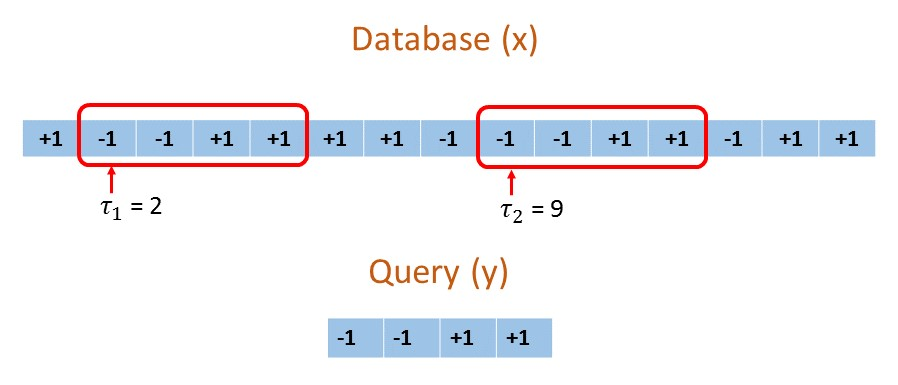
\includegraphics[width=2.8in]{Pattern_matching_ex.jpg}
	\end{figure}
	\vspace{-10pt}
	\begin{block}{}
\begin{itemize}\itemsep5pt
	\item {\color{blue} Database/String}: $\xv = [x[0], x[1], \cdots, x[N-1]]$ \ (length $N$)
	\item { \color{blue} Query/Substring}: $\yv = [y[0], y[1], \cdots, y[M-1]]$ \ (length $M = N^\mu$)
	\item {\color{blue} Signal Model:} $x[i]$'s are i.i.d ~ r.v. from $\mathcal{A} = \{+1,-1\}$ (extensions possible)
\end{itemize}
\end{block}

\vspace{-3pt}
\pause
\begin{block}{}
Determine all the {\color{blue} $L$ locations} $\underline{\tau} = [\tau_1, \tau_2, \cdots \tau_L]$ with  {\color{blue}high probability}  where
	\begin{enumerate}
		\item \alert{Exact Matching}:~  $\yv$ appears {\color{blue}exactly} in $\xv$
		\begin{itemize}
				\item [-]  $\yv := \xv[\tau:\tau+M-1]$
		\end{itemize}
        \pause
		\item \alert{Approximate Matching:} ~ $\yv$ is a {\color{blue}noisy substring} of $\xv$
		\begin{itemize}\itemsep3pt
				\item [-] $\yv := \xv[\tau:\tau+M-1] \odot \bv$
				\item [-] $\bv$ is a noise sequence with $d_H(\yv,\xv[\tau:\tau+M-1]) \leq K$
		\end{itemize}
	\end{enumerate}

	\end{block}
	 \end{frame}
% ----------------------------------------Notations---------------------------------------

\begin{frame}\frametitle{Notation}

	\begin{figure}[t]
		\centering
		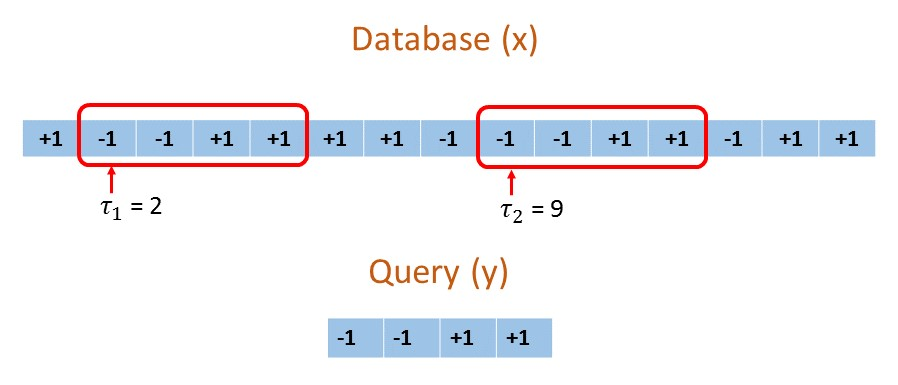
\includegraphics[width=2.5in]{Pattern_matching_ex.jpg}
	\end{figure}
	\vspace{-8pt}
	{\small
	\begin{table}[h!]
		\label{Table:Notations3}
		\begin{center}
			\begin{tabular}{|c|c|} 	
				\hline		
				\textit{Symbol}		&  \textit{Meaning} \\		
				\hline
				$N$           		& Size of the string or database in symbols \\
				\hline
				$M = N^{\mu}$       & Length of the query in symbols \\
				\hline
				$L = N^\lambda$    &   Number of matches \\
				\hline
				$K$             &$\max_{\tau}d_{H}(\xv[\tau:\tau+M-1],\yv)$\\
				\hline
				$\eta$             &$\frac{K}{M}$\\
				\hline
				%$G = N^\gamma$    & Number of blocks \\
				%\hline
				%$\tilde{N} = N^{1-\gamma}$   & Length of one block \\
				%\hline
				%$f_i = N^\alpha$     & Length of smaller point IDFT at each branch\\
				%\hline
				%$g_i = N/f_i$     	   &  Sub-sampling parameter \\
				%\hline
				%$B$   					    & Number of shifts also referred to as branches  \\
				%\hline
				%$d$           				& Number of stages in the FFAST algorithm \\
				%\hline
			\end{tabular}
		\end{center}
	\end{table}
    }
    \begin{block}{Probabilistic recovery}
    $\mbb{P}(\hat{\underline{\tau}} \neq \underline{\tau}) \rightarrow 0$ as $N \rightarrow \infty$
    \end{block}
	\end{frame}	
%------------------------------------------------------------------------------------------------------------
\begin{frame}\frametitle{Data vs Computing - Who's winning?}
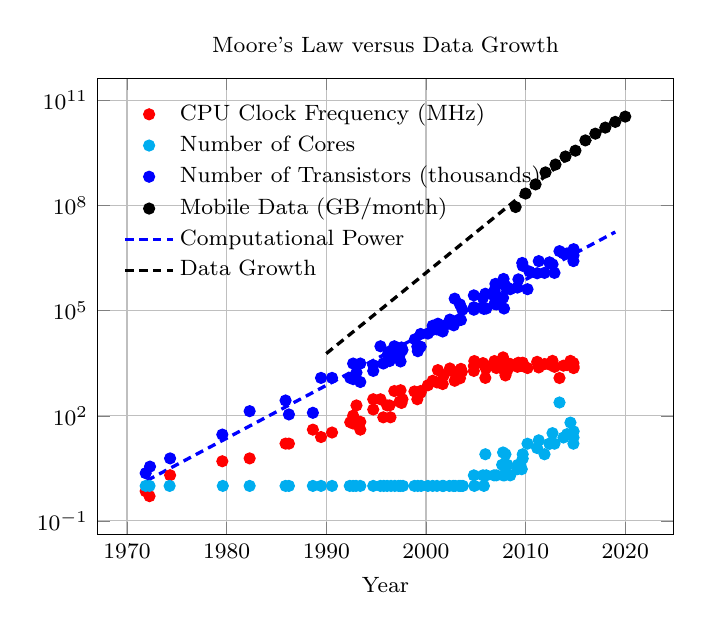
\begin{tikzpicture}
\pgfkeys{/pgf/number format/set thousands separator = {}}
\begin{semilogyaxis}[%
font=\footnotesize,
width=3.5in,
height=2.9in,
xmajorgrids,
ymajorgrids,
title={Moore's Law versus Data Growth},
xlabel={Year},
legend entries={CPU Clock Frequency (MHz), Number of Cores, Number of Transistors (thousands), Mobile Data (GB/month), Computational Power, Data Growth},
legend style={fill=none},
legend style={draw=none},
legend cell align=left,
legend pos=north west
]

%Time, Frequency
\addplot [color=red, mark=*, only marks]
coordinates {
(1971.875,0.704135515) (1972.259615,0.509367522) (1974.326923,2.016914555) (1979.567308,5.048065717) (1982.307692,6.097562352) (1985.913462,16.10761535) (1986.25,16.10761535) (1988.653846,40.31519363) (1989.471154,24.80454414) (1990.576923,33.37624694) (1992.403846,65.52488237) (1992.692308,60.42963902) (1992.692308,100.9035045) (1993.028846,198.0956779) (1993.413462,67.31703824) (1993.413462,40.31519363) (1994.711538,151.2472545) (1994.711538,296.9314848) (1995.432692,296.9314848) (1995.721154,90.57977759) (1996.105769,198.0956779) (1996.346154,198.0956779) (1996.442308,90.57977759) (1996.826923,509.3675217) (1997.355769,252.5478933) (1997.451923,537.6117475) (1997.548077,232.9096592) (1997.644231,296.9314848) (1998.846154,495.8068242) (1999.134615,296.9314848) (1999.182692,399.5420559) (1999.471154,457.2526699) (1999.471154,509.3675217) (2000.192308,743.1795488) (2000.673077,1000) (2001.105769,897.6871324) (2001.201923,2016.914555) (2001.682692,805.8421878) (2001.778846,1420.18117) (2002.403846,2246.790092) (2002.788462,1810.558243) (2002.884615,1000) (2003.413462,1175.743266) (2003.509615,2186.974655) (2003.605769,1810.558243) (2004.807692,2641.64832) (2004.807692,1910.952975) (2004.855769,3651.741273) (2005.721154,3190.848981) (2005.865385,2788.126665) (2005.961538,1207.900747) (2006.009615,2246.790092) (2006.875,3651.741273) (2006.875,2641.64832) (2007.019231,2713.899431) (2007.067308,2308.241527) (2007.644231,2942.727176) (2007.740385,4655.525931) (2007.740385,4067.944321) (2007.836538,2016.914555) (2007.980769,1420.18117) (2008.173077,2016.914555) (2008.173077,2308.241527) (2008.461538,3023.213025) (2009.182692,2502.865431) (2009.278846,3278.121151) (2009.423077,2641.64832) (2009.663462,2641.64832) (2009.711538,3278.121151) (2010.192308,2308.241527) (2011.16,3470) (2011.32,2400) (2011.9,3000) (2012.4,3100) (2012.41,2900) (2012.7,3700) (2012.9,2500) (2013.4,1200) (2013.8,2700) (2014.16,2800) (2014.5,3700) (2014.8,3200) (2014.81,2600) (2014.82,2300) };

%Time, Cores
\addplot [color=cyan, mark=*, only marks]
coordinates {
(1971.875,1) (1972.259615,1) (1974.278846,1) (1979.615385,1) (1982.307692,1) (1985.913462,1) (1986.25,1) (1988.653846,1) (1989.471154,1) (1990.576923,1) (1992.355769,1) (1992.692308,1) (1992.980769,1) (1993.413462,1) (1994.711538,1) (1995.432692,1) (1995.769231,1) (1996.105769,1) (1996.490385,1) (1996.875,1) (1997.259615,1) (1997.451923,1) (1997.692308,1) (1998.846154,1) (1999.182692,1) (1999.519231,1) (2000.192308,1) (2000.673077,1) (2001.105769,1) (2001.634615,1) (2001.778846,1) (2002.355769,1) (2002.740385,1) (2002.932692,1) (2003.317308,1) (2003.509615,1) (2003.701923,1) (2004.807692,2) (2004.855769,1) (2005.721154,2) (2005.817308,1) (2005.961538,8) (2006.057692,2) (2006.826923,2) (2007.067308,2) (2007.644231,4) (2007.740385,9) (2007.740385,2) (2007.884615,2) (2007.980769,8) (2008.173077,4) (2008.461538,2) (2009.182692,3) (2009.230769,4) (2009.471154,4) (2009.615385,3) (2009.711538,8) (2009.711538,6) (2010.192308,16) (2011.16,12) (2011.32,20) (2011.9,8) (2012.4,16) (2012.41,16) (2012.7,32) (2012.9,16) (2013.4,240) (2013.8,24) (2014.16,30) (2014.5,64) (2014.8,16) (2014.81,24) (2014.82,36) };


%Time, Transistors
\addplot [color=blue, mark=*, only marks]
coordinates {
(1971.875,2.308241527) (1972.307692,3.554522356) (1974.326923,6.097562352) (1979.567308,29.16377574) (1982.307692,135.7727142) (1985.913462,273.8419634) (1986.25,109.4113811) (1988.653846,121.8814185) (1989.471154,1207.900747) (1990.576923,1207.900747) (1992.403846,1207.900747) (1992.692308,3105.900224) (1992.692308,1113.97386) (1993.028846,1715.437896) (1993.413462,3105.900224) (1993.413462,922.2395651) (1994.711538,1910.952975) (1994.711538,2788.126665) (1995.432692,9646.616199) (1995.721154,3105.900224) (1996.153846,5473.703263) (1996.346154,6792.52507) (1996.346154,3651.741273) (1996.442308,4293.51021) (1996.826923,9646.616199) (1997.355769,5473.703263) (1997.451923,3554.522356) (1997.548077,8896.491128) (1997.644231,7566.695371) (1998.894231,15261.37803) (1999.134615,9389.79801) (1999.182692,6978.305849) (1999.471154,9389.79801) (1999.471154,21673.9217) (2000.192308,22266.7201) (2000.673077,28387.35965) (2000.673077,37180.26664) (2001.105769,29163.77574) (2001.201923,42550.65502) (2001.682692,25482.96748) (2001.826923,37180.26664) (2002.403846,55730.60401) (2002.788462,38197.17549) (2002.884615,220673.4069) (2003.413462,151247.2545) (2003.509615,54246.90937) (2003.653846,106498.5635) (2004.807692,125214.9689) (2004.807692,106498.5635) (2004.807692,273841.9634) (2005.721154,232909.6592) (2005.817308,112403.8664) (2005.961538,305052.789) (2006.057692,115478.1985) (2006.875,378551.5249) (2006.875,155383.9831) (2006.923077,245824.4069) (2006.971154,296931.4848) (2006.971154,582941.5347) (2007.067308,151247.2545) (2007.644231,582941.5347) (2007.740385,232909.6592) (2007.788462,805842.1878) (2007.836538,115478.1985) (2007.980769,509367.5217) (2008.221154,445079.4062) (2008.461538,410469.838) (2009.182692,457252.6699) (2009.278846,784388.5581) (2009.663462,2308241.527) (2009.711538,1910952.975) (2010.192308,410469.838) (2010.384615,1309747.264) (2011.16,1170000) (2011.32,2600000) (2011.9,1200000) (2012.4,2400000) (2012.41,2300000) (2012.7,2100000) (2012.9,1200000) (2013.4,5000000) (2013.8,4300000) (2014.16,4300000) (2014.5,4200000) (2014.8,2600000) (2014.81,3800000) (2014.82,5700000) };

\addplot [color=black, mark=*, only marks]
coordinates {
(2009, 91000000) (2010, 220000000) (2011, 402000000) (2012, 884000000) (2013, 1480000000) (2014, 2514000000) (2015, 3685000000) (2016, 7241000000) (2017, 11266000000) (2018, 16792000000) (2019, 24452000000) (2020, 34588000000) };

\addplot [color=blue, densely dashed, line width=1.2pt]
coordinates {
(1972, 1.42192406e+00) (1973, 2.01272654e+00) (1974, 2.84900455e+00) (1975, 4.03275198e+00) (1976, 5.70834066e+00) (1977, 8.08012823e+00) (1978, 1.14373819e+01) (1979, 1.61895580e+01) (1980, 2.29162401e+01) (1981, 3.24378255e+01) (1982, 4.59155830e+01) (1983, 6.49932828e+01) (1984, 9.19976733e+01) (1985, 1.30222256e+02) (1986, 1.84328965e+02) (1987, 2.60916746e+02) (1988, 3.69326375e+02) (1989, 5.22779674e+02) (1990, 7.39992067e+02) (1991, 1.04745514e+03) (1992, 1.48266762e+03) (1993, 2.09870875e+03) (1994, 2.97071196e+03) (1995, 4.20502822e+03) (1996, 5.95219683e+03) (1997, 8.42530545e+03) (1998, 1.19259786e+04) (1999, 1.68811642e+04) (2000, 2.38952052e+04) (2001, 3.38235459e+04) (2002, 4.78770634e+04) (2003, 6.77697486e+04) (2004, 9.59277471e+04) (2005, 1.35785256e+05) (2006, 1.92203364e+05) (2007, 2.72062920e+05) (2008, 3.85103730e+05) (2009, 5.45112443e+05) (2010, 7.71603991e+05) (2011, 1.09220167e+06) (2012, 1.54600611e+06) (2013, 2.18836407e+06) (2014, 3.09761862e+06) (2015, 4.38466397e+06) (2016, 6.20647036e+06) (2017, 8.78522838e+06) (2018, 1.24354477e+07) (2019, 1.76023153e+07)};

\addplot [color=black, densely dashed, line width=1.2pt]
coordinates {
(1990, 5.96878326e+03) (1991, 1.01461770e+04) (1992, 1.72472182e+04) (1993, 2.93180907e+04) (1994, 4.98370478e+04) (1995, 8.47166811e+04) (1996, 1.44007648e+05) (1997, 2.44794797e+05) (1998, 4.16120209e+05) (1999, 7.07351751e+05) (2000, 1.20240856e+06) (2001, 2.04394254e+06) (2002, 3.47444393e+06) (2003, 5.90611546e+06) (2004, 1.00396496e+07) (2005, 1.70661352e+07) (2006, 2.90102724e+07) (2007, 4.93137958e+07) (2008, 8.38272187e+07) (2009, 1.42495675e+08) (2010, 2.42224633e+08) (2011, 4.11751255e+08) (2012, 6.99925082e+08) (2013, 1.18978416e+09) (2014, 2.02248266e+09) (2015, 3.43796485e+09) (2016, 5.84410562e+09) (2017, 9.93424077e+09) (2018, 1.68869535e+10) (2019, 2.87056861e+10) };

\end{semilogyaxis}
\end{tikzpicture}
\pause
\begin{itemize}
\item Linear complexity is too expensive, sub-linear complexity is required
\end{itemize}

\end{frame}
%------------------------------------------------------------------------------------------------------------
\begin{frame}\frametitle{Big data applications}
\begin{block}{Metabolomics}
\begin{itemize}
  \item Database of genomes contains a sequence $\vec{x}$ of length $N=10^{6}-10^{12}$
\end{itemize}

\end{block}
  \begin{figure}[h]
  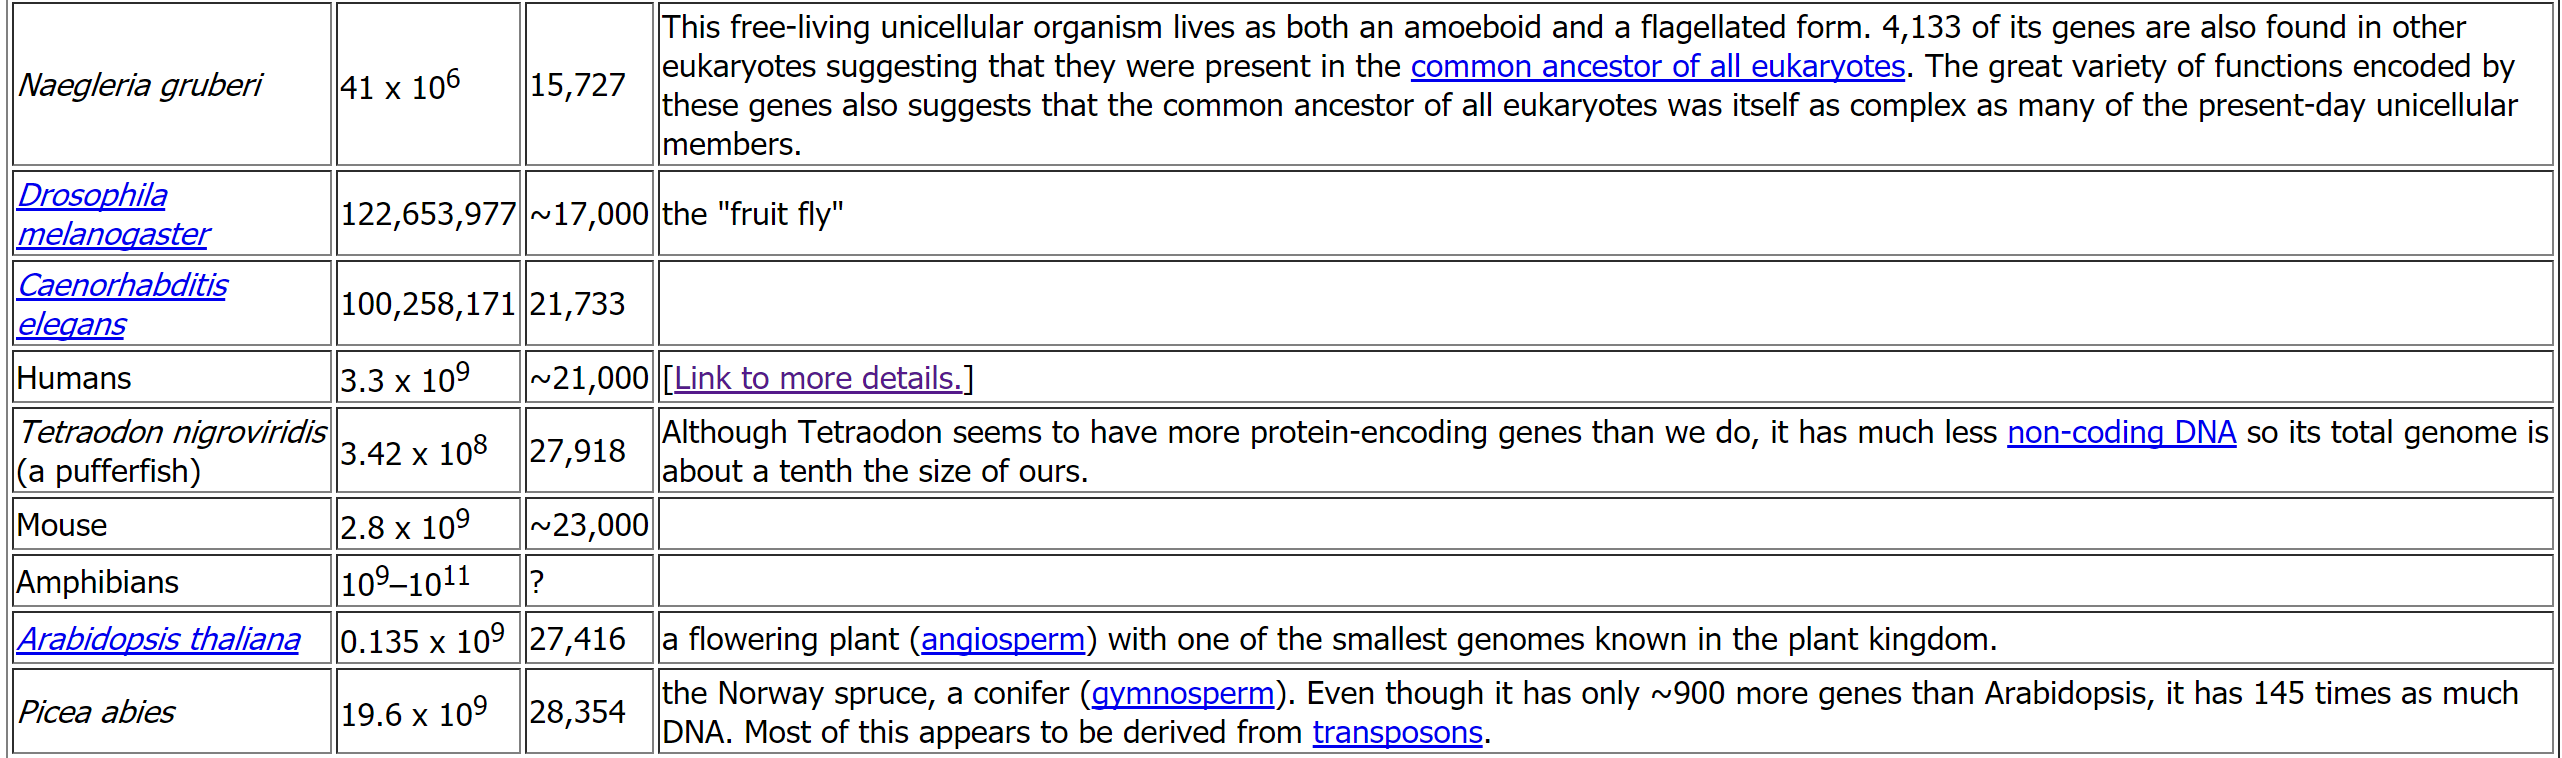
\includegraphics[width=4.0in]{genomesizes}
  \end{figure}

\url{http://www.biology-pages.info/G/GenomeSizes.html}
\end{frame}
%------------------------------------------------------------------------------------------------------------
\begin{frame}\frametitle{Big data applications}
\begin{block}{Metabolomics}
\begin{itemize}
  \item Database of genomes contains a sequence $\vec{x}$ of length $N=10^{6}-10^{12}$
  \item $M=1000$ to $M = 100000$ gives $\mu = 0.25$ to $\mu = 0.42$
\end{itemize}

  \begin{figure}[h]
  
\includegraphics[width=4.0in]{genomebiology}
  \end{figure}


\end{block}

\end{frame}
%------------------------------------------------------------------------------------------------------------
\begin{frame}\frametitle{Big data applications}
\begin{block}{Audio}
Let us consider the case of an audio signal which is sampled at a moderate sampling rate of $10$~KHz and let the signal $\xv$ correspond to 1 hour of audio and hence, $N = 3.6 \times 10^7$. Let the query $\yv$ be a 10 second clip which corresponds to $M = 10^4$ resulting in a $\mu = 0.529$.
\end{block}
\begin{block}{}
\begin{figure}
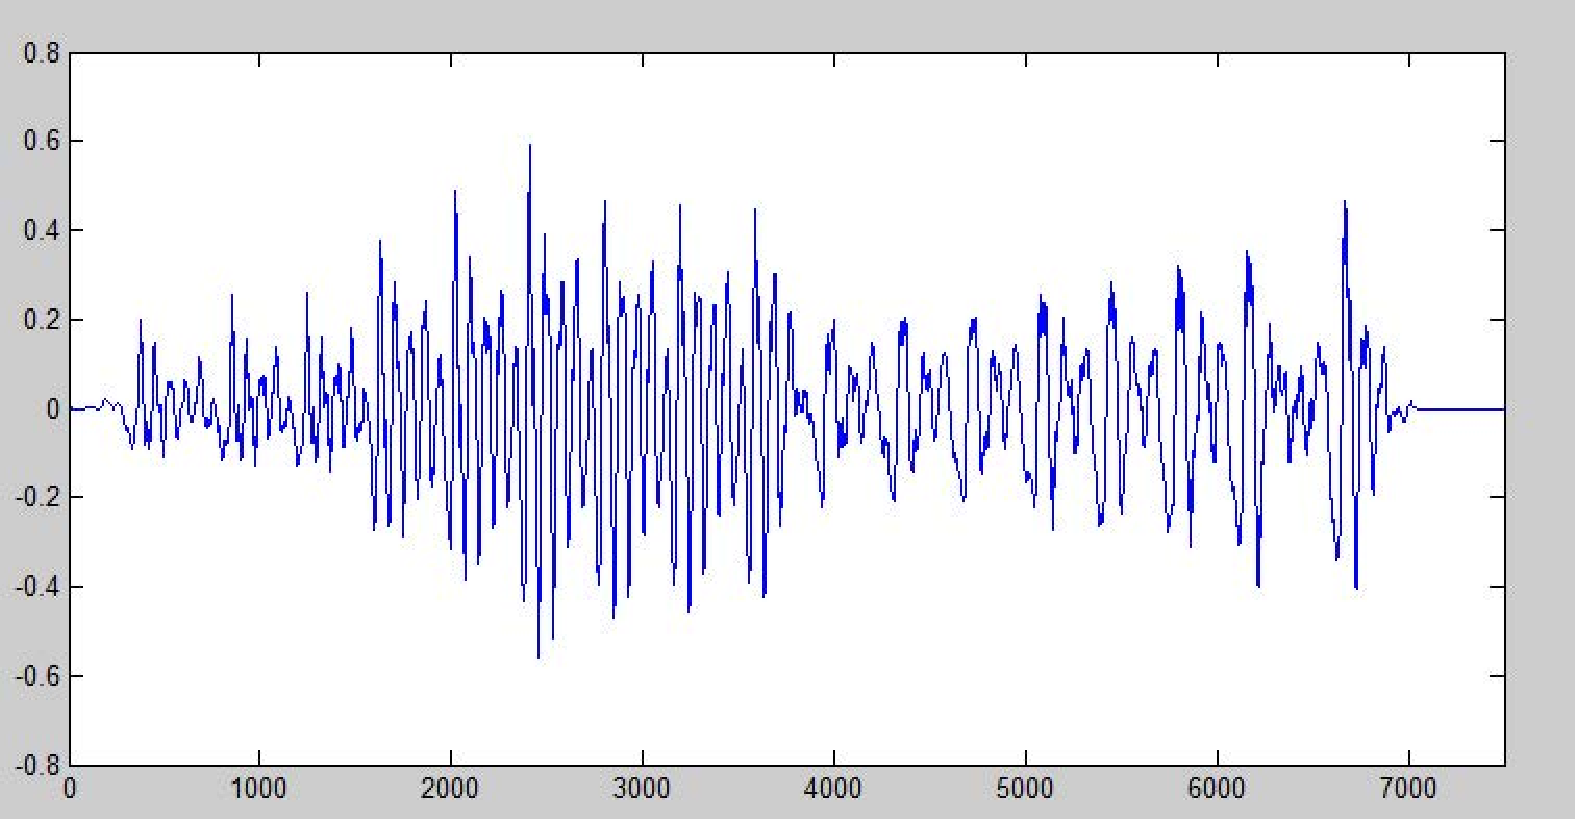
\includegraphics[width=3.5in]{ScaledVoice}
\end{figure}
\end{block}
\end{frame}
%%-------------------------------------------------------------------------------------------------------------

\begin{frame} \frametitle{Sketching Model}
		\vspace{-10pt}
	\begin{figure}
		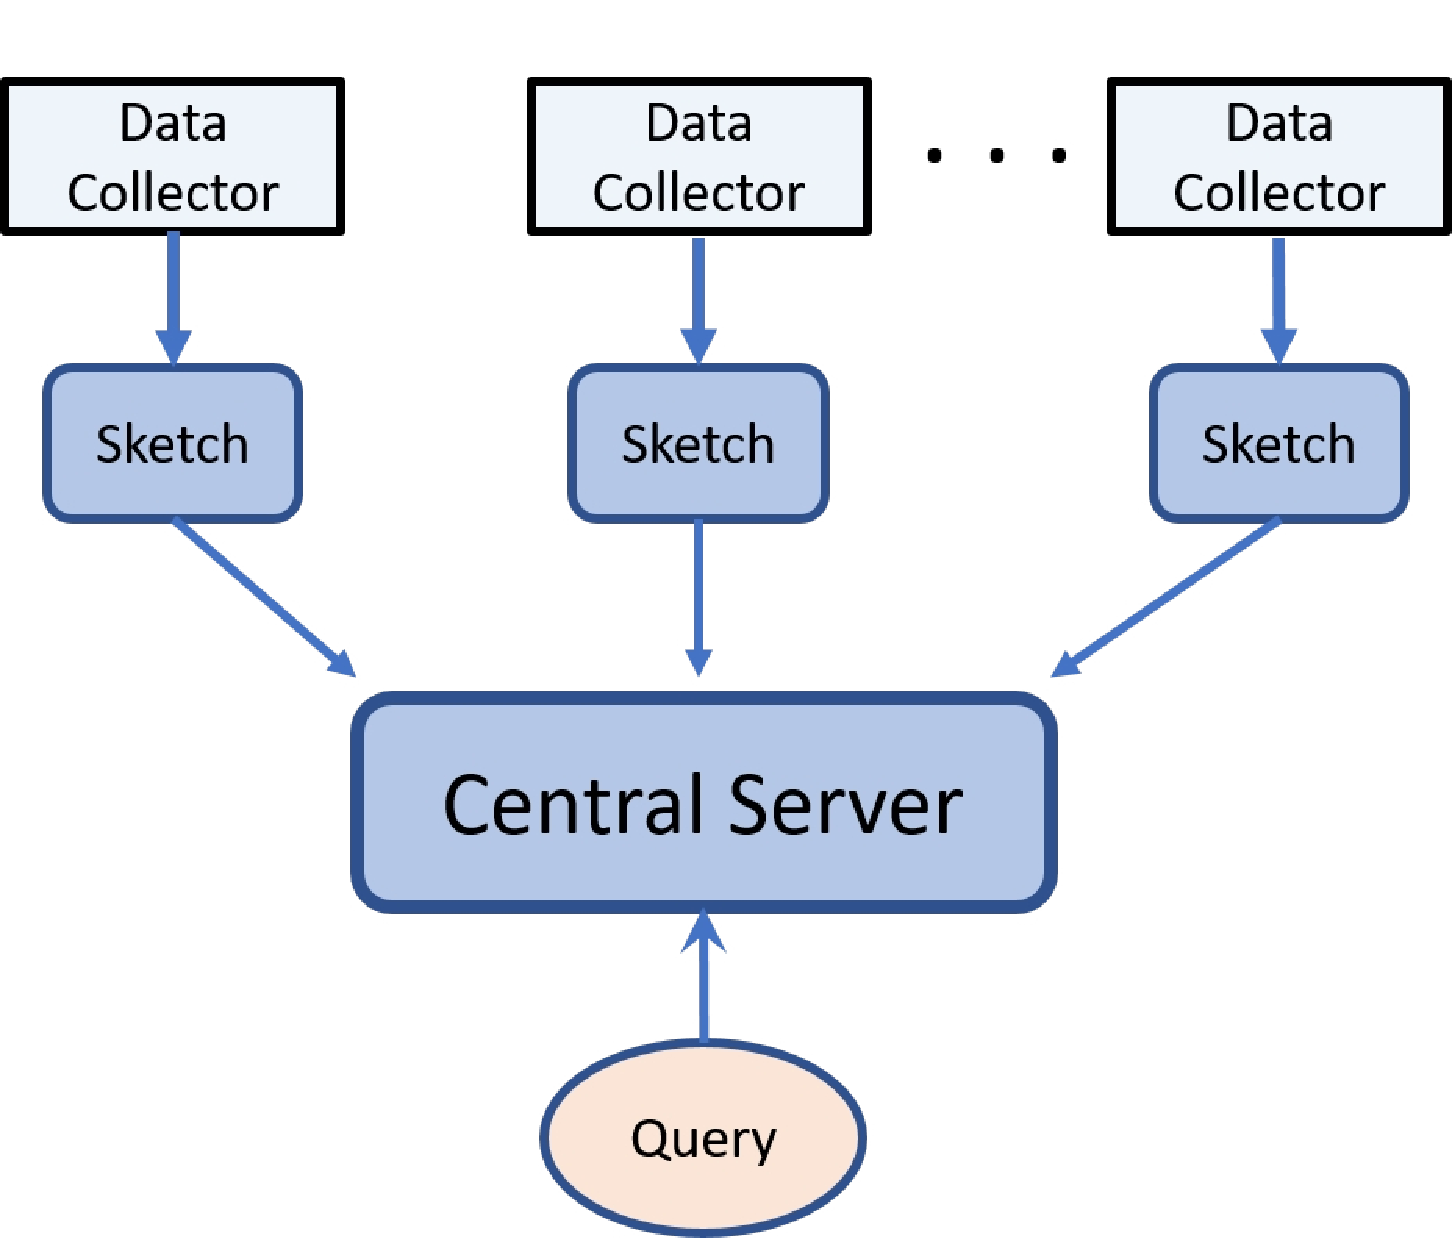
\includegraphics[width=2.5in]{SketchingModel}
	\end{figure}
	\vspace{-8pt}
	\begin{block}{Sketch}
		\begin{itemize}
			\item Succinct fingerprint (compressed form) of the data - min communication cost
			\item Allows Pattern Matching without decompression
			\item Could be both lossless or lossy (probabilistic recovery)
			\item \alert{Sketching Complexity} - space in bits to store the sketch of database
		\end{itemize}
	\end{block}
\end{frame}
%%-------------------------------------------------------------------------------------------------------------

\begin{frame} \frametitle{Lower Bounds on Sketching Complexity}
	\begin{block}{Exact Matching:}
		For a query of length $M = \Omega(\log N)$, any sketching algorithm that can determine the exact matches with a constant probability of error requires \alert{$s = \Omega(n-m)$} bits of memory
	\end{block}
	
	\begin{block}{Approximate Matching:}
		For a query of length $M$ and a Hamming distance $K= \eta M$ ($0<\eta<1$), any sketching algorithm that can determine the matches with a constant probability of error requires \alert{$s = \Omega (N/M \log N)$} bits of memory.
	\end{block}
	
	\begin{block}{Note}
		 Minor variations in the model\footfullcite{bar2004sketching} assumption and definition of error probability.
	\end{block}
\end{frame}
%%-------------------------------------------------------------------------------------------------------------
\begin{frame} \frametitle{Some Prior Work}
	\vspace{-0.2cm}
	 \begin{block}{Exact Matching - Non-sketching versions}	 	
	 	\begin{itemize}
            \item  {Rabin-Karp}: Match a set of strings - $O(N)$ complexity
	 		\item  {Boyer'77}: First occurrence of the match (only $\tau_1$)	 		
	 		\begin{itemize}
	 			\item[-] Average complexity - $O(N^{1-\mu} \log N)$ (sub-linear)
	 			\item[-] Worst case complexity - $O(N \log N)$
	 		\end{itemize}	
	 	\end{itemize}
	 \end{block}
	
	 \begin{block}{Exact Matching - Sketching versions - Bio informatics} 	
	 	\begin{itemize}
	 		\item  {Goodrich'05}: BWT, suffix-arrays based indexing
	 		\begin{itemize}
	 			\item[-] Time complexity - $O(M + L)$ (sub-linear)
	 			\item[-] Storage Complexity - $O(N~H_k(X) \log^\epsilon N) + o(N)$ bits  (linear)
	 			\item[-] Read alignment in Bio-informatics community[ {\color{blue}Li'09,Li'10}]
	 		\end{itemize}	 		
	 	\end{itemize}
	 \end{block}
\end{frame}
%-------------------------------------------------------------------------------------------------------------
\begin{frame} \frametitle{Some Prior Work}
	\vspace{-0.2cm}
	\begin{block}{\alert{Approximate Matching}}
		
	 	\begin{itemize}
	 		\item {Chang'94}: Generalization of Boyer'77
	 		\begin{itemize}
	 			\item[-] Average time complexity - $O(NK/M \log N)$ (sub-linear only when $K \ll M$ )
	 		\end{itemize}
	 		
	 		\item {Zhang'03}: Approximate Matching using BWT
	 			\begin{itemize}
	 				\item[-] Worst case time complexity: $O(\min\{M(M-K){|\mc{A}|}^k\log \frac{N}{|\mc{A}|} , NM \log \frac{N}{|\mc{A}|}\})$
	 				\item[-] Complexity grows with $|\mc{A}|$ and $K$
	 			\end{itemize}
	 		\pause	
	 		\item {Andoni'13}: $O\left(N^{1-0.359\mu}\right)$ (sub-linear even when $K = O(M)$)
	 		\begin{itemize}
	 			\item[-] Combinatorial in nature
	 		\end{itemize}
	 	\end{itemize}
	 	
	 \end{block}
\end{frame}
	
%---------------------------------------------------------------------------------------------------------------------------

%--------------------------------------------- Main Result -------------------------------------------------------------------
	 \begin{frame} \frametitle{Our Main Result}

	{\small
	\begin{table}[h!]
		\begin{center}
			\begin{tabular}{|c|c|} 	
				\hline		
				\textit{Symbol}		&  \textit{Meaning} \\		
				\hline
				$N$           		& Size of the string or database in symbols \\
				\hline
				$M = N^{\mu}$       & Length of the query in symbols \\
				\hline
				$L = N^\lambda$    &   Number of matches \\
				\hline
				$K$             &$\max_{\tau}d_{H}(\xv[\tau:\tau+M-1],\yv)$\\
				\hline
				$\eta$             &$\frac{K}{M}$\\
				\hline
			\end{tabular}
		\end{center}
	\end{table}
    }	
     	
    \vspace{-2.5mm}
	 \begin{theorem}
	 	Assume that a sketch of $\xv$ can be precomputed and stored. Then for the {\it exact pattern matching} and {\it approximate pattern matching} (with $K = \eta M,~ 0 \leq \eta \leq 1/6$) problems, our algorithm has
	 	\begin{itemize}
	 		\item \alert{Sketching complexity:} {\color{blue} $O(\frac{N}{M}\log N)=O(N^{1-\mu}\log N)$} \alert{samples}
	 		\item \alert{Computational complexity:}
	 		{\color{blue}$O(\max(N^{1-\mu}\log^2 N, N^{\mu+\lambda}\log N ))$}	 		
	 		\item a decoder for which $\mbb{P}(\hat{{\mathcal{T}}} \neq \mathcal{T}) \rightarrow 0$ as $N \rightarrow \infty$
	 	\end{itemize}
	 \end{theorem}
	 \pause
	 \vspace{-0.5mm}
	 \begin{block}{\alert{Note}}
	 	When $L<\frac{N}{M}$ (i.e. $\lambda<1-\mu$) our algorithm has a {\color{blue}sub-linear time} complexity.
	 \end{block}	
\end{frame}
%-------------------------------------------------------------------------------------------------------------
\begin{frame}\frametitle{Signal Processing View}

	\begin{figure}[t]
		\centering
		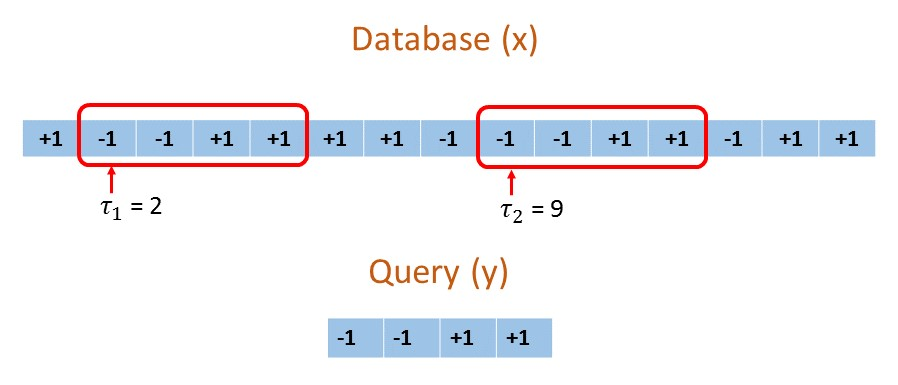
\includegraphics[width=3.5in]{Pattern_matching_ex.jpg}
	\end{figure}

			\begin{block}{}			
				\begin{itemize}
					\item {Cross-correlation} ($\rv$): $\displaystyle{r[m]=(\xv*\yv)[m] \defeq \sum_{i=0}^{M-1} x[m+i] y[i] }$
			        \pause
					\item {Naive implementation}: $O(MN) = O(N^{1+\mu})$ ({\color{blue} super-linear} complexity)
                    \pause
					\item {Fourier Transform Approach}: 1970's - $O(N \log N)$ complexity
					\begin{equation}\nonumber
					\rv = \mathcal{F}_{N}^{-1} \{~  \mathcal{F}_{N}\{\xv\} ~ \odot ~  \mathcal{F}_{N}\{\yv'\} ~ \}, \ \ \yv' = \yv^{*}[-n]
					\end{equation}
					
				\end{itemize}
			\end{block}												
\end{frame}
%-------------------------------------------------------------------------------------------------------------
\begin{frame}\frametitle{Main Idea}
	\vspace{-0.4cm}
			\begin{block}{}
			
				\begin{itemize}
					\item {Cross-correlation} ($\rv$):
					
                    \begin{eqnarray}
                    \nonumber
					r[m] & = & (\xv*\yv)[m] \defeq \sum_{i=0}^{M-1} x[m+i] y[i], ~ ~ \ 0 \leq m \leq N-1\\
                    \nonumber
					\rv  & = & \mathcal{F}_{N}^{-1} \{~  \mathcal{F}_{N}\{\xv\} ~ \odot ~  \mathcal{F}_{N}\{\yv'\} ~ \}, \ \ \yv' = \yv^{*}[-n]
					\end{eqnarray}					
				\end{itemize}
			\end{block}
			
				\begin{columns}
					\column{0.45\columnwidth}
			\begin{block}{\alert{ \bf Key Observation}}
			\vspace{0.2cm}
				\begin{itemize}
					\item $\rv$ is {\color{blue}Sparse} with some noise.
				\end{itemize}
				 \begin{equation} \label{eqn:RXY_sparse}\nonumber
				 r[m] \ = \left\{
				 \begin{array}{ll}
				 &M,~~  \text{if} \ m \in \mathcal{T} \\
				 & n_m,~~ m \in [N]-\mathcal{T}
				 \end{array}
				 \right.  			
				 \end{equation}
			\end{block}
						
					\column[]{0.45\columnwidth}
					\begin{figure}
						\centering
						\scalebox{0.35}{% This file was created by matlab2tikz.
%
%The latest updates can be retrieved from
%  http://www.mathworks.com/matlabcentral/fileexchange/22022-matlab2tikz-matlab2tikz
%where you can also make suggestions and rate matlab2tikz.
%
\definecolor{mycolor1}{rgb}{0.00000,0.44700,0.74100}%
%
\begin{tikzpicture}

\begin{axis}[%
width=4.521in,
height=3.566in,
at={(0.758in,0.481in)},
scale only axis,
xmin=0,
xmax=10000,
xlabel style={font=\color{white!20!black}},
xlabel={Samples},
xtick = {0,2000,4000,6000,8000,10000},
ymin=0,
ymax=100,
ylabel style={font=\color{white!20!black}},
ylabel={Magnitude of Cross-correlation $|R_{XY}|$},
ytick = {0,20,40,60,80,100},
axis background/.style={fill=white}
]
\addplot [color=mycolor1, forget plot, line width=1.5pt]
  table[row sep=crcr]{%
1	0\\
2	0\\
4	2\\
5	0\\
6	0\\
7	1\\
8	0\\
9	4\\
10	0\\
12	0\\
13	1\\
14	0\\
16	0\\
17	1\\
19	1\\
20	0\\
21	1\\
22	0\\
30	0\\
31	1\\
32	1\\
33	2\\
34	0\\
35	0\\
36	1\\
37	0\\
39	0\\
40	1\\
41	0\\
42	0\\
43	1\\
44	1\\
45	0\\
47	0\\
48	1\\
49	0\\
50	0\\
51	2\\
52	0\\
53	0\\
54	1\\
55	0\\
57	0\\
58	2\\
59	0\\
60	0\\
61	1\\
62	0\\
63	0\\
64	1\\
65	0\\
66	1\\
67	0\\
73	0\\
74	1\\
75	0\\
76	1\\
77	0\\
79	0\\
80	1\\
81	0\\
82	0\\
83	2\\
84	0\\
86	2\\
87	1\\
88	1\\
89	2\\
90	0\\
91	0\\
92	1\\
93	0\\
96	0\\
97	2\\
98	0\\
99	0\\
100	2\\
102	0\\
103	3\\
104	0\\
106	0\\
107	1\\
108	0\\
109	0\\
110	2\\
111	0\\
112	1\\
113	1\\
114	0\\
115	1\\
116	0\\
117	0\\
118	2\\
120	0\\
121	2\\
122	0\\
123	2\\
124	0\\
125	1\\
126	0\\
127	0\\
128	1\\
129	1\\
130	0\\
132	0\\
133	1\\
134	0\\
135	0\\
136	1\\
139	1\\
140	0\\
141	0\\
142	1\\
143	1\\
144	2\\
145	1\\
146	1\\
147	0\\
149	0\\
150	2\\
151	0\\
152	0\\
153	1\\
154	0\\
155	0\\
156	1\\
157	0\\
158	1\\
161	1\\
162	0\\
163	0\\
164	1\\
165	0\\
166	4\\
168	0\\
170	0\\
171	2\\
172	0\\
173	1\\
174	0\\
176	0\\
177	2\\
178	0\\
181	0\\
182	1\\
183	0\\
184	0\\
185	2\\
186	0\\
188	2\\
189	0\\
190	1\\
191	0\\
194	0\\
195	1\\
198	1\\
199	0\\
201	0\\
202	1\\
203	0\\
204	1\\
205	0\\
206	2\\
207	0\\
208	1\\
209	0\\
210	1\\
211	0\\
212	2\\
214	0\\
215	1\\
216	0\\
217	2\\
218	2\\
220	0\\
221	1\\
222	0\\
223	1\\
224	0\\
228	0\\
229	1\\
230	0\\
231	1\\
232	0\\
234	0\\
235	1\\
236	1\\
237	0\\
239	0\\
240	1\\
241	0\\
242	1\\
243	0\\
246	0\\
247	2\\
249	0\\
251	0\\
253	2\\
254	1\\
255	1\\
256	0\\
258	0\\
259	1\\
260	0\\
262	0\\
263	1\\
264	0\\
265	1\\
266	0\\
269	0\\
270	1\\
273	1\\
274	2\\
275	0\\
276	1\\
277	0\\
278	0\\
279	1\\
280	0\\
283	0\\
284	2\\
285	2\\
287	0\\
288	2\\
289	0\\
290	1\\
291	0\\
292	0\\
293	1\\
294	0\\
296	0\\
297	1\\
298	0\\
299	1\\
300	0\\
301	0\\
302	2\\
303	0\\
304	0\\
305	1\\
306	0\\
307	0\\
308	2\\
310	0\\
311	1\\
312	0\\
315	0\\
316	1\\
317	1\\
318	0\\
319	0\\
320	1\\
321	1\\
322	0\\
323	2\\
324	0\\
330	0\\
331	1\\
332	1\\
333	0\\
337	0\\
338	2\\
339	0\\
340	1\\
341	0\\
342	0\\
343	2\\
344	0\\
345	2\\
346	0\\
348	0\\
349	1\\
350	0\\
352	0\\
353	1\\
354	0\\
355	1\\
356	0\\
359	0\\
360	1\\
361	0\\
362	0\\
363	1\\
364	0\\
369	0\\
370	1\\
371	0\\
372	1\\
373	1\\
374	0\\
375	2\\
376	0\\
377	1\\
378	0\\
379	2\\
380	0\\
381	1\\
382	0\\
383	0\\
384	1\\
385	0\\
386	1\\
387	0\\
388	1\\
389	0\\
390	0\\
392	2\\
393	0\\
395	0\\
396	1\\
397	0\\
398	1\\
399	0\\
400	1\\
401	0\\
403	0\\
404	1\\
406	1\\
407	0\\
409	0\\
410	2\\
411	0\\
412	0\\
413	2\\
414	0\\
415	2\\
416	0\\
423	0\\
424	2\\
425	0\\
426	0\\
427	2\\
428	0\\
429	2\\
430	0\\
431	0\\
432	1\\
433	0\\
437	0\\
438	1\\
439	1\\
440	2\\
441	1\\
442	2\\
443	0\\
446	0\\
447	1\\
448	1\\
449	0\\
451	0\\
452	2\\
453	1\\
454	1\\
455	0\\
456	1\\
457	1\\
458	0\\
459	0\\
460	1\\
461	0\\
462	0\\
463	2\\
464	0\\
467	0\\
468	1\\
470	1\\
471	0\\
472	1\\
473	1\\
474	3\\
475	0\\
476	1\\
478	1\\
479	2\\
480	0\\
481	1\\
482	1\\
483	0\\
488	0\\
489	1\\
490	1\\
491	0\\
492	1\\
493	0\\
494	1\\
495	0\\
498	0\\
499	3\\
500	1\\
501	0\\
506	0\\
507	2\\
508	0\\
509	2\\
510	2\\
511	0\\
513	2\\
514	0\\
515	2\\
517	0\\
518	2\\
519	0\\
523	0\\
524	1\\
525	0\\
526	1\\
528	1\\
529	0\\
530	0\\
531	2\\
532	0\\
537	0\\
538	1\\
539	0\\
541	0\\
542	1\\
543	1\\
544	2\\
546	0\\
547	1\\
548	0\\
553	0\\
554	1\\
555	0\\
556	0\\
557	2\\
558	0\\
560	2\\
561	1\\
562	1\\
563	0\\
564	0\\
565	1\\
566	1\\
567	0\\
568	1\\
569	1\\
570	0\\
571	0\\
572	1\\
574	1\\
575	0\\
578	0\\
579	1\\
580	0\\
581	0\\
582	2\\
583	2\\
585	0\\
587	0\\
588	1\\
589	0\\
591	0\\
592	1\\
593	0\\
594	0\\
595	1\\
598	1\\
599	0\\
601	0\\
602	1\\
603	1\\
604	0\\
605	1\\
607	1\\
608	0\\
609	0\\
610	1\\
611	0\\
612	1\\
614	1\\
615	0\\
616	1\\
617	0\\
618	1\\
619	0\\
620	2\\
621	0\\
622	1\\
623	0\\
624	3\\
625	0\\
626	1\\
627	1\\
628	0\\
629	0\\
630	1\\
631	0\\
632	1\\
633	1\\
634	0\\
637	0\\
638	1\\
639	0\\
640	1\\
641	0\\
642	2\\
643	0\\
644	0\\
645	2\\
646	0\\
649	0\\
651	2\\
652	0\\
654	0\\
655	2\\
657	0\\
658	0\\
659	1\\
660	0\\
661	0\\
662	1\\
663	3\\
664	0\\
665	0\\
666	1\\
667	0\\
668	1\\
673	1\\
674	0\\
675	0\\
676	2\\
677	0\\
678	0\\
679	1\\
680	0\\
681	3\\
682	0\\
685	0\\
686	2\\
687	0\\
688	1\\
689	0\\
690	3\\
691	1\\
692	0\\
693	1\\
695	1\\
696	0\\
697	0\\
698	1\\
699	1\\
700	3\\
701	0\\
702	1\\
703	0\\
707	0\\
708	1\\
709	1\\
710	2\\
711	0\\
714	0\\
715	1\\
716	0\\
717	0\\
718	1\\
719	0\\
720	1\\
721	1\\
722	3\\
723	0\\
725	0\\
726	2\\
727	0\\
729	0\\
730	3\\
731	0\\
732	0\\
733	1\\
734	0\\
736	0\\
737	1\\
738	1\\
739	2\\
741	0\\
743	0\\
744	2\\
745	0\\
746	0\\
747	1\\
748	0\\
752	0\\
753	2\\
755	0\\
757	0\\
758	1\\
762	1\\
763	0\\
764	1\\
765	0\\
768	0\\
770	2\\
771	0\\
778	0\\
779	1\\
780	0\\
783	0\\
784	3\\
785	1\\
786	0\\
791	0\\
792	4\\
793	1\\
794	0\\
796	0\\
797	2\\
798	0\\
801	0\\
802	1\\
803	0\\
808	0\\
809	1\\
810	1\\
811	0\\
812	0\\
814	2\\
815	0\\
816	1\\
817	1\\
818	0\\
819	0\\
820	2\\
821	0\\
822	0\\
823	1\\
824	0\\
825	0\\
826	1\\
827	0\\
828	2\\
829	0\\
830	1\\
831	1\\
832	0\\
833	0\\
834	1\\
835	0\\
836	0\\
837	1\\
838	0\\
839	2\\
841	0\\
842	0\\
843	1\\
844	0\\
845	1\\
846	0\\
848	0\\
849	1\\
850	0\\
851	1\\
852	1\\
853	0\\
854	1\\
855	0\\
856	0\\
857	1\\
858	1\\
859	2\\
860	0\\
861	1\\
862	0\\
868	0\\
869	1\\
870	0\\
871	0\\
872	2\\
873	1\\
876	1\\
877	0\\
878	1\\
879	1\\
880	0\\
883	0\\
884	1\\
885	0\\
886	2\\
888	0\\
892	0\\
893	2\\
894	0\\
895	3\\
896	2\\
897	2\\
898	0\\
899	0\\
900	1\\
901	1\\
902	0\\
909	0\\
910	93\\
911	0\\
912	0\\
913	1\\
914	0\\
920	0\\
921	1\\
922	0\\
923	0\\
924	3\\
925	1\\
926	2\\
928	2\\
929	0\\
932	0\\
933	2\\
934	0\\
941	0\\
942	1\\
943	1\\
944	0\\
945	2\\
946	2\\
947	0\\
951	0\\
952	1\\
953	0\\
957	0\\
958	1\\
959	0\\
960	2\\
961	0\\
963	2\\
964	0\\
965	1\\
966	1\\
967	0\\
970	0\\
971	1\\
972	0\\
976	0\\
977	2\\
978	0\\
979	0\\
980	1\\
981	1\\
982	0\\
983	1\\
984	1\\
985	0\\
989	0\\
990	1\\
991	1\\
992	0\\
993	1\\
994	1\\
995	2\\
996	0\\
999	0\\
1000	3\\
1001	0\\
1004	0\\
1005	1\\
1006	0\\
1007	0\\
1008	1\\
1009	0\\
1010	1\\
1011	0\\
1012	1\\
1013	0\\
1014	1\\
1015	1\\
1016	0\\
1017	2\\
1018	0\\
1019	1\\
1020	0\\
1022	0\\
1023	1\\
1024	0\\
1025	0\\
1027	2\\
1029	0\\
1030	0\\
1031	1\\
1032	0\\
1033	1\\
1034	0\\
1035	0\\
1036	1\\
1037	0\\
1040	0\\
1041	1\\
1042	0\\
1044	2\\
1045	0\\
1046	0\\
1047	1\\
1048	1\\
1049	0\\
1050	1\\
1051	0\\
1052	1\\
1053	0\\
1054	1\\
1055	1\\
1056	0\\
1057	0\\
1058	1\\
1059	0\\
1063	0\\
1064	2\\
1065	0\\
1066	0\\
1067	2\\
1068	0\\
1071	0\\
1072	1\\
1073	1\\
1074	2\\
1075	0\\
1076	1\\
1077	0\\
1078	1\\
1079	0\\
1080	0\\
1082	2\\
1083	0\\
1084	2\\
1085	0\\
1092	0\\
1093	1\\
1094	0\\
1096	0\\
1097	2\\
1098	0\\
1099	0\\
1100	1\\
1101	0\\
1102	6\\
1103	1\\
1104	0\\
1105	1\\
1106	0\\
1107	0\\
1108	1\\
1109	0\\
1111	0\\
1112	1\\
1113	0\\
1115	0\\
1117	2\\
1118	0\\
1119	1\\
1120	0\\
1124	0\\
1125	1\\
1126	0\\
1130	0\\
1131	2\\
1132	0\\
1134	2\\
1136	0\\
1137	2\\
1139	0\\
1143	0\\
1144	1\\
1145	0\\
1151	0\\
1152	1\\
1153	1\\
1154	0\\
1156	0\\
1157	1\\
1158	0\\
1159	2\\
1160	0\\
1164	0\\
1165	2\\
1166	1\\
1167	1\\
1168	0\\
1169	1\\
1170	0\\
1174	0\\
1175	1\\
1176	0\\
1183	0\\
1184	1\\
1185	0\\
1186	2\\
1187	2\\
1188	0\\
1192	0\\
1193	1\\
1194	0\\
1196	0\\
1197	1\\
1198	0\\
1199	0\\
1200	2\\
1201	0\\
1202	1\\
1203	0\\
1206	0\\
1207	1\\
1208	0\\
1209	1\\
1212	1\\
1213	0\\
1214	1\\
1215	0\\
1216	1\\
1217	1\\
1218	0\\
1219	1\\
1220	0\\
1223	0\\
1224	1\\
1226	1\\
1227	0\\
1228	1\\
1229	0\\
1231	0\\
1232	1\\
1233	0\\
1237	0\\
1238	1\\
1239	0\\
1240	2\\
1241	0\\
1245	0\\
1246	1\\
1247	0\\
1248	0\\
1249	2\\
1250	0\\
1251	1\\
1252	0\\
1253	0\\
1254	1\\
1255	0\\
1257	0\\
1258	1\\
1259	0\\
1260	2\\
1261	1\\
1262	1\\
1263	0\\
1264	0\\
1265	2\\
1266	0\\
1267	0\\
1268	1\\
1269	0\\
1270	0\\
1271	2\\
1273	0\\
1274	3\\
1275	0\\
1276	0\\
1277	2\\
1278	0\\
1279	0\\
1280	2\\
1281	0\\
1282	2\\
1284	0\\
1285	0\\
1286	1\\
1287	0\\
1288	1\\
1289	0\\
1292	0\\
1293	1\\
1294	0\\
1297	0\\
1298	1\\
1299	0\\
1303	0\\
1304	1\\
1305	0\\
1306	1\\
1307	3\\
1308	1\\
1309	0\\
1317	0\\
1318	1\\
1319	1\\
1320	0\\
1321	0\\
1322	1\\
1323	0\\
1324	1\\
1325	0\\
1329	0\\
1330	1\\
1331	0\\
1332	1\\
1333	0\\
1334	1\\
1335	0\\
1338	0\\
1339	1\\
1341	1\\
1342	2\\
1343	0\\
1347	0\\
1348	1\\
1349	0\\
1350	0\\
1351	1\\
1352	3\\
1353	1\\
1354	1\\
1355	0\\
1356	0\\
1358	2\\
1359	0\\
1360	1\\
1361	0\\
1362	1\\
1363	0\\
1364	0\\
1365	1\\
1366	0\\
1370	0\\
1371	1\\
1372	1\\
1373	0\\
1374	0\\
1375	1\\
1376	0\\
1379	0\\
1380	1\\
1381	0\\
1382	1\\
1383	0\\
1384	0\\
1385	1\\
1386	0\\
1387	0\\
1389	2\\
1391	0\\
1392	1\\
1393	0\\
1396	0\\
1397	1\\
1398	0\\
1399	2\\
1400	0\\
1405	0\\
1406	2\\
1407	0\\
1413	0\\
1414	1\\
1415	1\\
1416	0\\
1422	0\\
1423	1\\
1424	0\\
1428	0\\
1429	1\\
1430	0\\
1431	0\\
1432	1\\
1433	1\\
1434	0\\
1436	0\\
1437	1\\
1438	0\\
1444	0\\
1445	1\\
1446	0\\
1447	2\\
1448	0\\
1450	0\\
1452	2\\
1453	0\\
1456	0\\
1458	2\\
1459	0\\
1460	1\\
1461	0\\
1463	0\\
1464	1\\
1465	0\\
1466	1\\
1468	1\\
1469	0\\
1470	1\\
1471	0\\
1476	0\\
1477	2\\
1478	0\\
1479	1\\
1480	0\\
1481	1\\
1482	1\\
1483	0\\
1484	0\\
1485	3\\
1486	1\\
1487	0\\
1491	0\\
1493	2\\
1494	2\\
1495	1\\
1496	1\\
1497	0\\
1498	1\\
1499	0\\
1500	0\\
1501	1\\
1502	0\\
1507	0\\
1508	1\\
1509	1\\
1510	0\\
1511	0\\
1512	1\\
1513	0\\
1514	1\\
1515	3\\
1516	1\\
1517	1\\
1518	0\\
1521	0\\
1522	2\\
1523	0\\
1525	0\\
1526	2\\
1527	0\\
1528	0\\
1529	1\\
1532	1\\
1533	0\\
1535	0\\
1536	2\\
1538	0\\
1539	0\\
1540	1\\
1541	1\\
1542	0\\
1543	0\\
1544	1\\
1546	1\\
1547	0\\
1548	1\\
1549	1\\
1550	0\\
1551	1\\
1552	3\\
1553	0\\
1554	2\\
1555	0\\
1560	0\\
1561	3\\
1562	0\\
1564	2\\
1566	0\\
1567	1\\
1570	1\\
1571	0\\
1573	0\\
1575	2\\
1576	0\\
1577	0\\
1578	3\\
1579	0\\
1580	1\\
1581	0\\
1582	1\\
1583	0\\
1584	3\\
1585	0\\
1588	0\\
1589	1\\
1590	1\\
1591	0\\
1592	1\\
1593	0\\
1596	0\\
1597	1\\
1598	0\\
1599	1\\
1600	0\\
1601	2\\
1602	0\\
1603	1\\
1604	0\\
1605	0\\
1606	1\\
1607	1\\
1608	0\\
1609	0\\
1610	1\\
1611	0\\
1614	0\\
1615	1\\
1616	0\\
1619	0\\
1620	1\\
1621	0\\
1633	0\\
1634	1\\
1635	0\\
1639	0\\
1640	1\\
1641	0\\
1642	0\\
1643	1\\
1644	0\\
1645	0\\
1646	1\\
1647	1\\
1648	0\\
1652	0\\
1653	1\\
1654	0\\
1657	0\\
1658	1\\
1659	0\\
1660	1\\
1661	0\\
1662	0\\
1663	1\\
1665	1\\
1666	0\\
1669	0\\
1670	1\\
1671	0\\
1673	0\\
1674	1\\
1675	0\\
1676	1\\
1677	0\\
1678	1\\
1679	1\\
1680	0\\
1681	1\\
1682	0\\
1689	0\\
1690	1\\
1691	4\\
1692	0\\
1695	0\\
1696	1\\
1697	1\\
1698	0\\
1700	0\\
1701	1\\
1702	0\\
1707	0\\
1708	1\\
1709	0\\
1716	0\\
1717	2\\
1718	1\\
1719	1\\
1720	0\\
1721	1\\
1722	0\\
1727	0\\
1728	1\\
1729	1\\
1730	0\\
1734	0\\
1735	1\\
1736	0\\
1739	0\\
1740	1\\
1741	0\\
1742	3\\
1743	0\\
1752	0\\
1753	1\\
1754	0\\
1755	0\\
1756	1\\
1757	0\\
1758	0\\
1759	1\\
1760	0\\
1761	0\\
1762	1\\
1763	0\\
1764	1\\
1765	1\\
1766	0\\
1767	1\\
1768	0\\
1769	0\\
1770	1\\
1771	0\\
1773	0\\
1774	1\\
1775	0\\
1777	0\\
1778	1\\
1779	1\\
1780	0\\
1781	2\\
1782	0\\
1790	0\\
1791	1\\
1792	0\\
1793	0\\
1794	1\\
1795	0\\
1799	0\\
1800	2\\
1801	0\\
1802	1\\
1803	0\\
1805	0\\
1806	1\\
1807	0\\
1808	1\\
1809	3\\
1810	0\\
1811	1\\
1812	0\\
1813	2\\
1814	0\\
1817	0\\
1818	1\\
1819	1\\
1820	0\\
1821	1\\
1822	0\\
1825	0\\
1826	1\\
1827	0\\
1828	1\\
1829	0\\
1831	0\\
1832	1\\
1833	0\\
1834	0\\
1835	1\\
1836	0\\
1841	0\\
1842	1\\
1843	0\\
1845	0\\
1846	1\\
1848	1\\
1849	0\\
1850	2\\
1851	0\\
1852	1\\
1853	0\\
1859	0\\
1860	1\\
1861	0\\
1862	0\\
1863	1\\
1864	0\\
1865	1\\
1866	0\\
1869	0\\
1870	1\\
1871	0\\
1877	0\\
1878	1\\
1880	1\\
1881	0\\
1882	1\\
1883	0\\
1886	0\\
1887	1\\
1888	0\\
1889	1\\
1890	0\\
1891	0\\
1892	1\\
1893	1\\
1894	0\\
1895	1\\
1896	0\\
1897	2\\
1898	0\\
1899	1\\
1900	0\\
1903	0\\
1904	1\\
1905	0\\
1910	0\\
1912	2\\
1913	0\\
1914	1\\
1915	0\\
1917	0\\
1918	1\\
1919	0\\
1920	2\\
1921	0\\
1922	0\\
1923	1\\
1924	0\\
1925	1\\
1926	0\\
1927	4\\
1928	1\\
1929	0\\
1930	0\\
1931	1\\
1932	0\\
1933	0\\
1934	2\\
1935	0\\
1936	1\\
1937	0\\
1938	0\\
1939	1\\
1940	0\\
1943	0\\
1944	2\\
1945	0\\
1948	0\\
1949	1\\
1950	1\\
1951	0\\
1953	2\\
1955	0\\
1956	1\\
1957	0\\
1959	0\\
1960	1\\
1961	0\\
1962	1\\
1963	0\\
1968	0\\
1969	3\\
1970	0\\
1971	1\\
1972	0\\
1973	1\\
1974	0\\
1975	1\\
1976	1\\
1977	4\\
1978	0\\
1981	0\\
1982	1\\
1983	0\\
1986	0\\
1988	2\\
1989	0\\
1990	1\\
1991	0\\
1992	0\\
1993	2\\
1994	0\\
1997	0\\
1998	1\\
1999	0\\
2003	0\\
2004	2\\
2005	1\\
2006	1\\
2007	0\\
2009	0\\
2010	1\\
2011	0\\
2012	2\\
2013	0\\
2016	0\\
2017	1\\
2018	0\\
2024	0\\
2025	1\\
2026	0\\
2027	0\\
2028	1\\
2029	0\\
2030	2\\
2031	0\\
2032	1\\
2033	0\\
2034	2\\
2035	0\\
2036	1\\
2037	1\\
2038	0\\
2041	0\\
2042	1\\
2043	0\\
2046	0\\
2047	3\\
2048	0\\
2057	0\\
2058	1\\
2059	0\\
2060	1\\
2061	1\\
2062	0\\
2068	0\\
2069	1\\
2070	0\\
2071	1\\
2072	0\\
2076	0\\
2077	3\\
2079	3\\
2080	1\\
2081	0\\
2082	0\\
2083	1\\
2084	0\\
2087	0\\
2088	1\\
2089	0\\
2090	0\\
2091	1\\
2092	1\\
2093	0\\
2095	0\\
2096	1\\
2097	1\\
2098	0\\
2107	0\\
2108	1\\
2109	0\\
2110	0\\
2111	1\\
2112	0\\
2113	0\\
2114	1\\
2115	0\\
2124	0\\
2125	1\\
2126	0\\
2127	1\\
2128	0\\
2129	1\\
2131	1\\
2133	3\\
2134	0\\
2135	0\\
2136	1\\
2137	0\\
2139	0\\
2140	1\\
2141	1\\
2142	0\\
2146	0\\
2147	1\\
2148	0\\
2149	0\\
2150	1\\
2151	0\\
2152	1\\
2153	0\\
2154	0\\
2155	1\\
2156	0\\
2160	0\\
2161	1\\
2162	0\\
2163	0\\
2164	1\\
2165	0\\
2166	1\\
2167	0\\
2168	0\\
2169	1\\
2170	0\\
2171	0\\
2172	1\\
2173	0\\
2178	0\\
2179	2\\
2180	0\\
2181	0\\
2182	1\\
2183	0\\
2191	0\\
2192	1\\
2193	0\\
2197	0\\
2198	1\\
2199	0\\
2207	0\\
2208	2\\
2209	0\\
2212	0\\
2213	1\\
2214	0\\
2219	0\\
2220	1\\
2221	0\\
2223	0\\
2224	1\\
2225	1\\
2226	0\\
2227	0\\
2228	2\\
2229	0\\
2230	1\\
2231	0\\
2237	0\\
2238	3\\
2239	0\\
2240	1\\
2241	0\\
2242	0\\
2243	1\\
2244	0\\
2245	2\\
2246	0\\
2247	1\\
2248	0\\
2249	0\\
2250	1\\
2252	1\\
2253	0\\
2255	0\\
2256	1\\
2257	1\\
2258	0\\
2259	1\\
2260	0\\
2262	0\\
2263	2\\
2264	0\\
2266	0\\
2267	1\\
2268	0\\
2270	0\\
2271	2\\
2272	1\\
2273	1\\
2274	0\\
2276	0\\
2277	1\\
2278	0\\
2280	0\\
2281	1\\
2282	0\\
2283	0\\
2284	1\\
2285	0\\
2286	1\\
2287	0\\
2289	0\\
2290	1\\
2291	1\\
2292	0\\
2293	0\\
2295	2\\
2296	0\\
2298	0\\
2299	1\\
2300	0\\
2303	0\\
2304	1\\
2306	1\\
2307	0\\
2308	2\\
2309	0\\
2310	1\\
2311	0\\
2312	0\\
2313	1\\
2314	0\\
2316	0\\
2317	1\\
2318	0\\
2319	1\\
2320	0\\
2321	1\\
2322	0\\
2325	0\\
2326	3\\
2327	1\\
2328	0\\
2329	0\\
2330	2\\
2331	0\\
2333	0\\
2334	3\\
2335	0\\
2337	0\\
2338	1\\
2339	0\\
2340	1\\
2341	1\\
2342	0\\
2343	1\\
2344	0\\
2345	1\\
2346	0\\
2347	1\\
2348	1\\
2349	0\\
2352	0\\
2353	1\\
2354	0\\
2356	0\\
2357	1\\
2358	0\\
2360	0\\
2361	3\\
2362	1\\
2363	0\\
2366	0\\
2367	1\\
2368	0\\
2369	2\\
2370	2\\
2371	0\\
2372	0\\
2373	1\\
2374	0\\
2375	1\\
2376	0\\
2377	0\\
2378	3\\
2379	0\\
2380	1\\
2381	0\\
2382	1\\
2383	0\\
2384	0\\
2385	1\\
2386	0\\
2389	0\\
2390	1\\
2391	1\\
2392	0\\
2396	0\\
2397	1\\
2399	1\\
2400	0\\
2404	0\\
2405	1\\
2406	0\\
2407	0\\
2408	2\\
2409	1\\
2411	1\\
2412	0\\
2413	1\\
2414	0\\
2415	0\\
2416	1\\
2417	0\\
2419	0\\
2421	2\\
2422	0\\
2436	0\\
2437	1\\
2438	0\\
2445	0\\
2446	1\\
2447	0\\
2451	0\\
2452	1\\
2453	0\\
2459	0\\
2461	2\\
2462	0\\
2467	0\\
2468	1\\
2469	0\\
2472	0\\
2473	2\\
2474	0\\
2475	0\\
2476	1\\
2477	0\\
2478	0\\
2479	1\\
2480	0\\
2481	2\\
2482	0\\
2483	1\\
2484	0\\
2485	0\\
2486	4\\
2487	0\\
2492	0\\
2493	1\\
2494	0\\
2495	0\\
2496	1\\
2499	1\\
2500	3\\
2501	0\\
2503	0\\
2504	2\\
2505	0\\
2507	0\\
2508	2\\
2510	0\\
2511	1\\
2512	0\\
2516	0\\
2517	1\\
2518	1\\
2519	3\\
2520	4\\
2521	0\\
2522	2\\
2523	3\\
2524	0\\
2526	0\\
2527	1\\
2528	0\\
2529	1\\
2530	0\\
2531	2\\
2532	0\\
2535	0\\
2536	1\\
2537	0\\
2538	1\\
2539	0\\
2540	0\\
2541	1\\
2542	0\\
2543	0\\
2544	4\\
2545	0\\
2549	0\\
2550	1\\
2551	0\\
2552	0\\
2553	1\\
2554	0\\
2558	0\\
2559	1\\
2560	0\\
2562	0\\
2563	2\\
2564	0\\
2565	0\\
2566	1\\
2567	1\\
2568	0\\
2569	1\\
2570	1\\
2571	0\\
2572	0\\
2573	1\\
2574	1\\
2575	0\\
2576	1\\
2577	0\\
2579	2\\
2580	2\\
2581	0\\
2582	1\\
2583	0\\
2584	2\\
2586	0\\
2587	1\\
2588	0\\
2590	0\\
2591	1\\
2592	0\\
2593	1\\
2594	0\\
2595	0\\
2596	1\\
2597	0\\
2599	2\\
2600	0\\
2601	0\\
2602	1\\
2603	1\\
2604	0\\
2605	0\\
2606	1\\
2607	0\\
2610	0\\
2612	2\\
2614	0\\
2615	1\\
2616	1\\
2617	0\\
2619	0\\
2620	1\\
2622	1\\
2623	0\\
2625	0\\
2626	2\\
2627	0\\
2628	1\\
2629	1\\
2630	0\\
2631	0\\
2632	2\\
2634	0\\
2635	0\\
2636	2\\
2637	0\\
2638	1\\
2639	0\\
2642	0\\
2643	1\\
2644	1\\
2645	0\\
2646	1\\
2647	0\\
2648	0\\
2650	2\\
2651	0\\
2652	0\\
2653	1\\
2654	0\\
2656	0\\
2657	1\\
2658	1\\
2659	0\\
2662	0\\
2663	2\\
2664	1\\
2668	1\\
2669	0\\
2670	1\\
2671	0\\
2674	0\\
2675	2\\
2676	0\\
2677	2\\
2678	0\\
2679	1\\
2680	1\\
2681	0\\
2691	0\\
2693	2\\
2694	0\\
2695	0\\
2696	1\\
2697	1\\
2698	0\\
2699	2\\
2700	0\\
2701	1\\
2702	0\\
2703	1\\
2704	0\\
2705	0\\
2706	1\\
2707	1\\
2708	0\\
2709	0\\
2710	3\\
2711	0\\
2712	1\\
2713	0\\
2715	0\\
2716	1\\
2717	3\\
2718	0\\
2719	0\\
2720	2\\
2721	0\\
2722	2\\
2723	0\\
2724	0\\
2725	1\\
2726	0\\
2727	2\\
2729	0\\
2730	1\\
2731	3\\
2732	2\\
2733	0\\
2735	0\\
2736	1\\
2737	1\\
2738	0\\
2739	0\\
2740	2\\
2741	0\\
2742	0\\
2743	1\\
2744	0\\
2747	0\\
2748	1\\
2749	4\\
2750	0\\
2753	0\\
2754	1\\
2755	1\\
2756	2\\
2757	0\\
2758	2\\
2759	0\\
2760	3\\
2761	0\\
2764	0\\
2766	2\\
2767	0\\
2768	2\\
2769	0\\
2770	1\\
2771	0\\
2772	1\\
2773	0\\
2775	0\\
2776	2\\
2777	1\\
2778	1\\
2779	0\\
2780	2\\
2782	0\\
2783	1\\
2784	0\\
2785	1\\
2786	0\\
2788	0\\
2789	1\\
2790	0\\
2792	0\\
2793	1\\
2794	0\\
2795	1\\
2796	0\\
2798	0\\
2799	1\\
2800	0\\
2801	1\\
2802	0\\
2803	1\\
2804	0\\
2805	0\\
2807	2\\
2808	0\\
2809	1\\
2810	0\\
2811	1\\
2812	1\\
2813	0\\
2814	0\\
2815	1\\
2816	1\\
2817	0\\
2818	0\\
2819	1\\
2820	0\\
2821	1\\
2822	0\\
2823	0\\
2824	2\\
2825	3\\
2826	0\\
2827	1\\
2828	0\\
2829	1\\
2830	0\\
2831	2\\
2832	0\\
2833	1\\
2834	0\\
2835	2\\
2836	0\\
2837	1\\
2838	0\\
2841	0\\
2842	1\\
2843	1\\
2844	0\\
2845	1\\
2846	0\\
2847	1\\
2848	0\\
2849	2\\
2850	0\\
2851	0\\
2852	2\\
2854	0\\
2855	1\\
2856	1\\
2857	0\\
2859	0\\
2860	3\\
2861	0\\
2868	0\\
2869	1\\
2870	1\\
2871	0\\
2873	0\\
2874	3\\
2875	1\\
2876	2\\
2877	2\\
2878	0\\
2879	0\\
2881	2\\
2882	0\\
2883	0\\
2884	1\\
2885	0\\
2886	0\\
2888	2\\
2889	1\\
2890	1\\
2891	0\\
2892	1\\
2893	0\\
2895	0\\
2896	1\\
2897	0\\
2898	1\\
2899	0\\
2900	2\\
2901	0\\
2902	1\\
2903	0\\
2904	0\\
2905	2\\
2906	0\\
2907	0\\
2908	3\\
2909	0\\
2911	0\\
2912	2\\
2913	0\\
2914	0\\
2915	1\\
2916	1\\
2917	0\\
2919	0\\
2921	2\\
2923	0\\
2928	0\\
2929	4\\
2930	0\\
2931	0\\
2932	1\\
2933	1\\
2934	0\\
2935	1\\
2936	0\\
2937	0\\
2938	2\\
2939	1\\
2940	1\\
2941	0\\
2942	0\\
2944	2\\
2945	0\\
2951	0\\
2952	2\\
2953	0\\
2956	0\\
2958	2\\
2959	1\\
2960	1\\
2961	0\\
2962	1\\
2963	1\\
2964	0\\
2965	0\\
2966	1\\
2967	1\\
2968	0\\
2970	0\\
2971	1\\
2972	0\\
2974	0\\
2975	2\\
2977	0\\
2978	1\\
2979	0\\
2983	0\\
2984	1\\
2985	0\\
2986	1\\
2987	1\\
2988	0\\
2989	2\\
2990	0\\
2991	0\\
2992	1\\
2993	0\\
2994	0\\
2995	5\\
2996	0\\
3002	0\\
3003	1\\
3004	1\\
3005	0\\
3006	0\\
3007	3\\
3008	1\\
3009	0\\
3010	1\\
3011	1\\
3012	0\\
3022	0\\
3024	2\\
3025	0\\
3026	3\\
3028	1\\
3029	1\\
3030	0\\
3032	0\\
3033	1\\
3034	0\\
3037	0\\
3038	1\\
3039	0\\
3040	0\\
3041	1\\
3042	0\\
3044	0\\
3045	1\\
3046	0\\
3047	0\\
3048	1\\
3049	0\\
3050	1\\
3051	0\\
3055	0\\
3056	1\\
3057	1\\
3058	0\\
3059	2\\
3060	0\\
3061	0\\
3062	2\\
3063	0\\
3064	2\\
3065	0\\
3066	3\\
3067	1\\
3068	1\\
3069	0\\
3070	1\\
3071	0\\
3074	0\\
3075	1\\
3076	0\\
3077	1\\
3078	0\\
3079	1\\
3080	1\\
3081	0\\
3083	0\\
3084	1\\
3085	0\\
3086	0\\
3087	2\\
3088	0\\
3089	1\\
3091	1\\
3092	0\\
3093	1\\
3094	0\\
3097	0\\
3098	1\\
3099	0\\
3101	2\\
3103	0\\
3104	2\\
3106	0\\
3108	2\\
3109	0\\
3110	1\\
3111	1\\
3112	2\\
3113	0\\
3118	0\\
3119	2\\
3120	0\\
3121	1\\
3122	0\\
3123	0\\
3124	1\\
3125	0\\
3126	0\\
3127	2\\
3128	1\\
3129	2\\
3131	0\\
3132	0\\
3133	3\\
3134	0\\
3135	1\\
3136	0\\
3137	0\\
3138	1\\
3139	0\\
3140	1\\
3144	1\\
3145	0\\
3146	0\\
3147	3\\
3148	0\\
3149	0\\
3150	3\\
3151	0\\
3152	0\\
3153	1\\
3154	0\\
3158	0\\
3159	1\\
3160	3\\
3161	0\\
3164	0\\
3165	2\\
3166	0\\
3173	0\\
3174	1\\
3175	0\\
3177	0\\
3178	1\\
3179	0\\
3182	0\\
3183	1\\
3184	0\\
3191	0\\
3192	1\\
3193	0\\
3196	0\\
3197	1\\
3198	1\\
3199	0\\
3200	2\\
3201	0\\
3202	0\\
3203	1\\
3204	0\\
3212	0\\
3213	1\\
3214	1\\
3215	0\\
3216	1\\
3217	3\\
3218	0\\
3222	0\\
3223	1\\
3224	1\\
3225	0\\
3227	2\\
3228	2\\
3229	0\\
3230	1\\
3231	1\\
3232	0\\
3233	0\\
3234	1\\
3235	0\\
3241	0\\
3242	1\\
3243	0\\
3244	3\\
3245	1\\
3246	1\\
3247	0\\
3251	0\\
3252	1\\
3253	0\\
3254	1\\
3255	0\\
3256	1\\
3257	0\\
3258	1\\
3259	1\\
3260	0\\
3261	0\\
3262	1\\
3263	0\\
3264	2\\
3265	0\\
3266	1\\
3267	0\\
3271	0\\
3272	1\\
3273	1\\
3274	0\\
3275	2\\
3276	2\\
3277	0\\
3278	1\\
3279	1\\
3280	3\\
3281	1\\
3283	1\\
3284	0\\
3286	0\\
3287	1\\
3288	1\\
3289	0\\
3293	0\\
3294	2\\
3295	0\\
3296	0\\
3297	3\\
3298	0\\
3300	0\\
3301	1\\
3302	0\\
3304	0\\
3305	1\\
3306	0\\
3308	0\\
3309	1\\
3310	0\\
3311	1\\
3312	0\\
3313	1\\
3314	1\\
3315	0\\
3316	1\\
3317	1\\
3318	0\\
3322	0\\
3323	1\\
3324	0\\
3325	0\\
3326	3\\
3329	0\\
3330	0\\
3331	2\\
3332	0\\
3333	1\\
3334	0\\
3335	1\\
3336	1\\
3337	2\\
3338	0\\
3339	2\\
3341	0\\
3342	1\\
3343	0\\
3344	2\\
3345	0\\
3348	0\\
3349	2\\
3350	0\\
3357	0\\
3358	1\\
3359	0\\
3361	0\\
3362	1\\
3363	1\\
3364	0\\
3365	0\\
3366	1\\
3367	0\\
3368	1\\
3369	0\\
3370	0\\
3371	1\\
3372	0\\
3380	0\\
3381	1\\
3382	0\\
3387	0\\
3388	1\\
3389	0\\
3390	1\\
3391	0\\
3400	0\\
3401	1\\
3402	1\\
3403	0\\
3404	0\\
3405	1\\
3406	0\\
3407	1\\
3408	0\\
3415	0\\
3416	2\\
3417	0\\
3418	1\\
3419	0\\
3420	0\\
3421	1\\
3422	0\\
3423	0\\
3425	2\\
3426	0\\
3427	2\\
3428	0\\
3429	0\\
3430	2\\
3432	0\\
3435	0\\
3436	2\\
3438	0\\
3439	1\\
3440	0\\
3441	1\\
3442	1\\
3443	0\\
3444	1\\
3446	1\\
3447	0\\
3448	2\\
3449	0\\
3454	0\\
3455	2\\
3456	0\\
3457	1\\
3458	1\\
3459	2\\
3460	0\\
3461	1\\
3462	0\\
3465	0\\
3466	1\\
3467	0\\
3468	0\\
3469	1\\
3470	0\\
3471	0\\
3472	1\\
3473	0\\
3474	1\\
3475	0\\
3476	1\\
3477	1\\
3478	0\\
3479	1\\
3480	0\\
3482	0\\
3483	1\\
3485	1\\
3486	0\\
3487	0\\
3488	1\\
3489	1\\
3490	0\\
3492	0\\
3493	2\\
3494	0\\
3495	0\\
3496	1\\
3497	1\\
3498	0\\
3500	2\\
3501	0\\
3502	1\\
3503	0\\
3504	0\\
3505	1\\
3507	1\\
3508	0\\
3509	1\\
3510	0\\
3512	2\\
3513	0\\
3514	1\\
3515	1\\
3516	0\\
3527	0\\
3528	1\\
3529	1\\
3530	0\\
3532	0\\
3533	1\\
3534	0\\
3535	3\\
3536	0\\
3537	1\\
3538	0\\
3540	0\\
3541	1\\
3542	0\\
3543	1\\
3545	1\\
3546	0\\
3547	1\\
3548	1\\
3549	3\\
3550	0\\
3551	1\\
3553	1\\
3554	0\\
3556	0\\
3557	1\\
3558	1\\
3559	2\\
3561	0\\
3565	0\\
3566	1\\
3567	0\\
3568	2\\
3570	0\\
3572	0\\
3573	4\\
3574	0\\
3576	0\\
3577	1\\
3578	0\\
3579	1\\
3580	1\\
3581	0\\
3582	0\\
3583	2\\
3584	2\\
3585	0\\
3586	0\\
3587	1\\
3588	1\\
3589	0\\
3592	0\\
3593	1\\
3594	1\\
3595	0\\
3596	0\\
3597	1\\
3598	0\\
3601	0\\
3602	1\\
3603	0\\
3604	0\\
3605	2\\
3606	0\\
3610	0\\
3611	1\\
3612	0\\
3613	0\\
3614	1\\
3615	0\\
3616	1\\
3617	0\\
3618	0\\
3619	2\\
3621	0\\
3624	0\\
3625	1\\
3626	1\\
3627	0\\
3628	1\\
3629	1\\
3630	0\\
3635	0\\
3636	2\\
3637	1\\
3638	1\\
3639	0\\
3640	1\\
3641	1\\
3642	0\\
3645	0\\
3646	1\\
3647	1\\
3648	0\\
3650	0\\
3651	4\\
3652	0\\
3653	2\\
3654	0\\
3655	1\\
3656	0\\
3657	1\\
3658	0\\
3663	0\\
3664	2\\
3665	0\\
3666	1\\
3667	0\\
3668	1\\
3669	0\\
3671	0\\
3672	2\\
3673	0\\
3674	0\\
3675	1\\
3676	0\\
3677	1\\
3678	0\\
3679	1\\
3680	0\\
3681	3\\
3682	1\\
3683	0\\
3685	0\\
3686	1\\
3687	0\\
3688	0\\
3689	1\\
3690	0\\
3691	0\\
3692	1\\
3693	0\\
3697	0\\
3698	1\\
3699	0\\
3701	0\\
3702	2\\
3704	0\\
3706	0\\
3707	1\\
3708	0\\
3709	0\\
3710	2\\
3712	0\\
3713	0\\
3714	2\\
3715	0\\
3716	0\\
3717	2\\
3718	1\\
3719	1\\
3720	0\\
3722	0\\
3723	1\\
3724	0\\
3730	0\\
3731	1\\
3732	0\\
3733	1\\
3734	1\\
3735	0\\
3736	1\\
3737	0\\
3739	0\\
3740	1\\
3741	0\\
3743	0\\
3744	1\\
3745	0\\
3746	3\\
3747	0\\
3748	0\\
3749	1\\
3750	0\\
3751	1\\
3752	0\\
3753	1\\
3754	0\\
3757	0\\
3758	1\\
3759	0\\
3763	0\\
3764	1\\
3765	0\\
3766	1\\
3767	3\\
3768	0\\
3770	2\\
3771	0\\
3772	1\\
3773	0\\
3779	0\\
3780	3\\
3781	1\\
3782	0\\
3783	0\\
3784	3\\
3785	0\\
3786	1\\
3787	0\\
3788	0\\
3789	1\\
3790	1\\
3791	0\\
3792	1\\
3793	0\\
3795	2\\
3796	1\\
3798	1\\
3799	2\\
3800	0\\
3802	0\\
3803	1\\
3804	0\\
3805	0\\
3806	1\\
3807	0\\
3808	0\\
3809	1\\
3812	1\\
3813	0\\
3815	0\\
3816	1\\
3817	0\\
3818	1\\
3819	0\\
3820	0\\
3822	2\\
3824	0\\
3825	1\\
3826	0\\
3827	1\\
3828	0\\
3831	0\\
3832	1\\
3833	0\\
3834	1\\
3835	1\\
3836	0\\
3842	0\\
3843	1\\
3844	0\\
3846	0\\
3847	2\\
3848	0\\
3849	0\\
3850	1\\
3852	1\\
3853	0\\
3854	0\\
3855	2\\
3856	0\\
3857	1\\
3858	0\\
3859	0\\
3860	1\\
3861	0\\
3862	1\\
3863	0\\
3865	0\\
3866	4\\
3867	1\\
3868	1\\
3869	0\\
3870	2\\
3871	2\\
3872	0\\
3873	0\\
3874	2\\
3875	0\\
3876	1\\
3877	0\\
3878	2\\
3880	0\\
3881	1\\
3882	0\\
3883	1\\
3884	1\\
3885	2\\
3886	0\\
3889	0\\
3890	1\\
3891	0\\
3892	2\\
3893	0\\
3894	0\\
3895	2\\
3896	0\\
3898	0\\
3899	1\\
3900	0\\
3901	0\\
3902	3\\
3903	0\\
3905	0\\
3907	2\\
3909	0\\
3911	0\\
3912	1\\
3914	1\\
3915	0\\
3918	0\\
3919	4\\
3920	0\\
3921	2\\
3922	0\\
3927	0\\
3928	2\\
3929	0\\
3930	1\\
3931	1\\
3932	0\\
3935	0\\
3936	1\\
3939	1\\
3940	0\\
3947	0\\
3948	1\\
3949	0\\
3950	1\\
3951	0\\
3953	0\\
3954	1\\
3955	1\\
3956	0\\
3963	0\\
3964	1\\
3967	1\\
3968	0\\
3969	1\\
3970	1\\
3971	0\\
3972	0\\
3973	1\\
3974	1\\
3975	0\\
3977	0\\
3978	1\\
3979	0\\
3981	0\\
3982	1\\
3983	1\\
3984	0\\
3985	0\\
3986	2\\
3988	0\\
3990	0\\
3991	1\\
3994	1\\
3995	0\\
3996	2\\
3997	0\\
3999	0\\
4000	1\\
4001	0\\
4002	1\\
4003	0\\
4005	0\\
4006	1\\
4007	3\\
4008	1\\
4009	0\\
4011	0\\
4012	1\\
4013	0\\
4019	0\\
4020	1\\
4021	0\\
4022	3\\
4023	1\\
4024	0\\
4026	2\\
4027	0\\
4029	0\\
4031	2\\
4032	0\\
4034	0\\
4035	1\\
4036	1\\
4037	0\\
4038	3\\
4039	1\\
4040	1\\
4041	0\\
4044	0\\
4045	1\\
4046	0\\
4047	0\\
4048	1\\
4049	0\\
4050	0\\
4051	1\\
4052	0\\
4053	1\\
4054	0\\
4057	0\\
4058	1\\
4059	0\\
4060	2\\
4061	1\\
4062	4\\
4063	1\\
4064	0\\
4068	0\\
4069	1\\
4070	1\\
4071	0\\
4072	0\\
4073	1\\
4074	0\\
4076	0\\
4077	2\\
4079	0\\
4082	0\\
4083	1\\
4084	0\\
4085	0\\
4086	1\\
4087	0\\
4088	1\\
4089	0\\
4090	2\\
4092	0\\
4096	0\\
4097	1\\
4098	1\\
4099	0\\
4100	0\\
4101	2\\
4102	0\\
4103	1\\
4104	1\\
4105	0\\
4110	0\\
4111	2\\
4112	1\\
4113	1\\
4114	2\\
4115	2\\
4116	1\\
4117	1\\
4118	0\\
4120	0\\
4121	1\\
4122	0\\
4124	0\\
4125	1\\
4126	0\\
4127	0\\
4129	2\\
4130	0\\
4131	1\\
4132	0\\
4133	2\\
4134	0\\
4137	0\\
4139	2\\
4140	0\\
4141	0\\
4142	2\\
4143	1\\
4144	2\\
4145	0\\
4146	1\\
4147	0\\
4154	0\\
4155	1\\
4156	4\\
4157	0\\
4158	1\\
4159	1\\
4160	0\\
4167	0\\
4168	1\\
4169	1\\
4170	2\\
4171	0\\
4175	0\\
4176	1\\
4177	0\\
4178	0\\
4179	1\\
4180	0\\
4181	1\\
4182	0\\
4184	0\\
4185	1\\
4186	0\\
4187	0\\
4188	1\\
4189	0\\
4191	0\\
4192	1\\
4193	0\\
4196	0\\
4198	2\\
4199	0\\
4202	0\\
4203	2\\
4204	0\\
4205	0\\
4206	1\\
4207	0\\
4208	1\\
4210	1\\
4211	0\\
4217	0\\
4218	1\\
4219	0\\
4222	0\\
4223	4\\
4224	0\\
4227	0\\
4228	1\\
4229	0\\
4230	1\\
4231	1\\
4232	0\\
4233	0\\
4234	3\\
4235	0\\
4236	1\\
4237	1\\
4238	0\\
4239	0\\
4240	3\\
4241	1\\
4242	0\\
4243	1\\
4244	0\\
4245	1\\
4246	0\\
4248	0\\
4250	2\\
4251	0\\
4252	0\\
4253	1\\
4254	1\\
4255	0\\
4258	0\\
4259	1\\
4260	0\\
4261	0\\
4262	1\\
4263	0\\
4264	2\\
4265	0\\
4267	0\\
4268	2\\
4269	0\\
4270	0\\
4271	1\\
4272	0\\
4274	0\\
4276	2\\
4277	1\\
4278	2\\
4279	1\\
4280	1\\
4281	0\\
4282	1\\
4283	0\\
4284	0\\
4285	2\\
4287	0\\
4289	0\\
4290	1\\
4291	0\\
4292	1\\
4293	1\\
4294	0\\
4295	1\\
4296	0\\
4297	1\\
4299	1\\
4300	0\\
4302	0\\
4303	1\\
4304	0\\
4306	2\\
4307	0\\
4308	1\\
4309	0\\
4310	1\\
4311	0\\
4312	3\\
4313	1\\
4314	0\\
4316	2\\
4317	2\\
4318	0\\
4319	1\\
4321	1\\
4322	0\\
4325	0\\
4327	2\\
4328	0\\
4329	2\\
4330	0\\
4331	1\\
4334	1\\
4335	0\\
4336	0\\
4337	1\\
4338	1\\
4339	0\\
4340	1\\
4341	0\\
4342	0\\
4343	1\\
4344	0\\
4346	2\\
4347	1\\
4348	2\\
4349	0\\
4350	0\\
4351	2\\
4352	0\\
4353	0\\
4354	1\\
4355	0\\
4359	0\\
4360	1\\
4362	1\\
4363	2\\
4364	0\\
4365	1\\
4366	0\\
4367	0\\
4368	1\\
4369	0\\
4370	1\\
4371	0\\
4372	1\\
4373	1\\
4374	0\\
4375	1\\
4376	0\\
4377	0\\
4378	1\\
4379	1\\
4380	0\\
4381	0\\
4382	1\\
4383	0\\
4387	0\\
4388	1\\
4389	1\\
4390	0\\
4395	0\\
4396	1\\
4397	0\\
4398	0\\
4399	3\\
4400	2\\
4401	4\\
4402	0\\
4410	0\\
4411	1\\
4412	0\\
4415	0\\
4416	2\\
4417	0\\
4423	0\\
4424	1\\
4425	0\\
4429	0\\
4430	1\\
4432	1\\
4433	0\\
4434	0\\
4435	1\\
4436	0\\
4437	0\\
4438	1\\
4439	0\\
4441	0\\
4442	1\\
4443	0\\
4446	0\\
4447	1\\
4448	1\\
4449	0\\
4451	0\\
4452	2\\
4453	0\\
4454	1\\
4455	0\\
4456	1\\
4457	0\\
4458	1\\
4459	0\\
4461	0\\
4462	3\\
4463	1\\
4464	1\\
4465	0\\
4466	0\\
4467	2\\
4469	0\\
4470	0\\
4471	1\\
4472	1\\
4473	3\\
4474	0\\
4475	3\\
4476	0\\
4479	0\\
4481	2\\
4482	0\\
4484	0\\
4485	2\\
4486	0\\
4488	2\\
4489	1\\
4490	1\\
4491	0\\
4493	0\\
4495	2\\
4497	0\\
4502	0\\
4503	1\\
4504	0\\
4505	1\\
4506	0\\
4507	0\\
4508	2\\
4510	0\\
4511	1\\
4512	7\\
4513	1\\
4514	2\\
4515	0\\
4516	1\\
4517	0\\
4518	1\\
4519	0\\
4520	0\\
4521	1\\
4522	1\\
4523	0\\
4524	0\\
4525	1\\
4526	0\\
4527	1\\
4528	1\\
4529	0\\
4530	1\\
4532	1\\
4533	0\\
4537	0\\
4538	4\\
4539	0\\
4540	0\\
4541	1\\
4543	1\\
4544	0\\
4545	1\\
4546	0\\
4547	2\\
4548	1\\
4549	2\\
4550	5\\
4551	0\\
4554	0\\
4555	1\\
4556	0\\
4557	1\\
4558	0\\
4559	1\\
4560	0\\
4563	0\\
4564	2\\
4565	2\\
4567	0\\
4568	0\\
4570	2\\
4571	0\\
4573	0\\
4574	1\\
4575	0\\
4576	1\\
4577	0\\
4578	1\\
4579	0\\
4581	0\\
4582	1\\
4583	0\\
4584	0\\
4585	2\\
4587	0\\
4592	0\\
4593	4\\
4594	0\\
4596	2\\
4597	1\\
4598	1\\
4599	0\\
4600	1\\
4601	0\\
4602	2\\
4604	0\\
4605	1\\
4606	1\\
4607	2\\
4608	0\\
4609	0\\
4610	1\\
4611	0\\
4613	0\\
4614	1\\
4615	0\\
4617	0\\
4618	1\\
4619	0\\
4621	2\\
4622	1\\
4623	1\\
4624	0\\
4628	0\\
4629	1\\
4630	0\\
4631	6\\
4632	0\\
4635	0\\
4636	1\\
4637	0\\
4638	0\\
4639	1\\
4640	0\\
4645	0\\
4647	2\\
4648	0\\
4649	0\\
4650	1\\
4651	0\\
4652	0\\
4653	2\\
4654	0\\
4655	1\\
4656	0\\
4657	0\\
4658	1\\
4661	1\\
4662	0\\
4663	0\\
4664	1\\
4665	3\\
4666	0\\
4667	3\\
4668	0\\
4669	0\\
4670	2\\
4671	0\\
4673	0\\
4674	1\\
4675	0\\
4676	0\\
4677	1\\
4678	0\\
4679	2\\
4680	0\\
4681	1\\
4682	1\\
4683	0\\
4686	0\\
4687	1\\
4688	0\\
4693	0\\
4694	2\\
4696	0\\
4698	0\\
4699	2\\
4700	1\\
4701	2\\
4702	0\\
4703	1\\
4704	0\\
4705	2\\
4706	0\\
4708	0\\
4709	3\\
4710	1\\
4713	1\\
4714	2\\
4716	0\\
4717	0\\
4718	1\\
4719	0\\
4722	0\\
4723	1\\
4724	1\\
4725	2\\
4726	0\\
4727	0\\
4728	1\\
4729	3\\
4730	0\\
4731	1\\
4732	1\\
4733	0\\
4734	1\\
4735	0\\
4740	0\\
4742	2\\
4743	0\\
4746	0\\
4747	1\\
4748	0\\
4749	1\\
4750	1\\
4751	0\\
4753	0\\
4754	1\\
4755	0\\
4756	2\\
4757	0\\
4764	0\\
4765	1\\
4767	1\\
4768	0\\
4769	1\\
4771	1\\
4772	0\\
4773	2\\
4774	0\\
4775	0\\
4776	1\\
4777	1\\
4778	0\\
4779	1\\
4781	1\\
4782	0\\
4783	0\\
4785	2\\
4786	2\\
4787	0\\
4788	0\\
4789	2\\
4790	0\\
4791	1\\
4792	0\\
4793	1\\
4794	0\\
4796	0\\
4797	4\\
4798	0\\
4799	0\\
4800	1\\
4801	1\\
4802	2\\
4803	1\\
4804	1\\
4805	0\\
4808	0\\
4809	1\\
4810	0\\
4811	2\\
4812	0\\
4814	0\\
4815	1\\
4816	0\\
4817	2\\
4818	2\\
4819	0\\
4820	0\\
4821	1\\
4822	0\\
4825	0\\
4826	1\\
4827	1\\
4828	3\\
4829	1\\
4830	0\\
4832	0\\
4833	3\\
4834	1\\
4835	0\\
4837	0\\
4838	1\\
4840	1\\
4841	2\\
4843	0\\
4845	0\\
4847	2\\
4848	0\\
4849	0\\
4850	1\\
4851	0\\
4852	1\\
4854	1\\
4855	0\\
4858	0\\
4859	3\\
4860	4\\
4861	0\\
4862	2\\
4863	1\\
4864	1\\
4865	2\\
4866	0\\
4867	1\\
4868	0\\
4871	0\\
4872	1\\
4873	0\\
4874	0\\
4875	2\\
4877	0\\
4881	0\\
4882	3\\
4883	1\\
4887	1\\
4888	2\\
4889	1\\
4890	1\\
4891	0\\
4893	0\\
4894	2\\
4895	0\\
4897	2\\
4898	0\\
4899	1\\
4900	3\\
4901	0\\
4902	2\\
4903	0\\
4904	1\\
4905	0\\
4906	0\\
4907	1\\
4908	0\\
4910	0\\
4911	2\\
4912	0\\
4916	0\\
4917	1\\
4918	0\\
4919	0\\
4920	2\\
4921	0\\
4922	4\\
4923	0\\
4924	1\\
4925	1\\
4926	0\\
4929	0\\
4930	1\\
4931	0\\
4932	0\\
4933	2\\
4934	0\\
4935	3\\
4936	1\\
4937	2\\
4939	0\\
4940	1\\
4941	0\\
4946	0\\
4947	1\\
4948	0\\
4950	0\\
4951	3\\
4952	0\\
4954	2\\
4955	0\\
4956	0\\
4957	1\\
4958	0\\
4959	1\\
4960	0\\
4964	0\\
4965	1\\
4966	1\\
4967	0\\
4971	0\\
4972	3\\
4973	0\\
4974	2\\
4975	0\\
4977	0\\
4978	1\\
4979	0\\
4982	0\\
4983	1\\
4984	0\\
4985	2\\
4987	0\\
4988	0\\
4989	3\\
4990	0\\
4993	0\\
4994	1\\
4995	0\\
4996	0\\
4997	1\\
4998	0\\
5001	0\\
5002	1\\
5003	0\\
5004	1\\
5006	1\\
5007	0\\
5008	1\\
5009	0\\
5012	0\\
5013	1\\
5014	0\\
5015	1\\
5016	0\\
5017	1\\
5018	1\\
5019	3\\
5020	0\\
5021	1\\
5022	0\\
5024	2\\
5025	0\\
5027	0\\
5028	1\\
5029	0\\
5030	1\\
5031	0\\
5034	0\\
5035	1\\
5036	0\\
5042	0\\
5043	1\\
5044	0\\
5046	0\\
5047	1\\
5048	0\\
5049	1\\
5050	0\\
5051	0\\
5052	1\\
5053	0\\
5054	2\\
5055	0\\
5056	3\\
5057	0\\
5060	0\\
5061	1\\
5062	0\\
5068	0\\
5069	1\\
5070	0\\
5072	0\\
5073	1\\
5075	1\\
5076	2\\
5077	0\\
5078	1\\
5079	0\\
5086	0\\
5087	1\\
5088	0\\
5089	2\\
5091	0\\
5093	0\\
5094	1\\
5095	0\\
5097	0\\
5098	1\\
5099	0\\
5105	0\\
5106	1\\
5109	1\\
5110	0\\
5111	1\\
5112	0\\
5114	0\\
5115	1\\
5116	0\\
5118	0\\
5120	2\\
5121	0\\
5122	0\\
5123	2\\
5124	0\\
5125	1\\
5128	1\\
5129	0\\
5130	1\\
5131	0\\
5133	0\\
5134	1\\
5135	0\\
5138	0\\
5140	2\\
5142	0\\
5144	0\\
5145	1\\
5146	0\\
5148	0\\
5149	2\\
5151	0\\
5152	0\\
5153	1\\
5154	0\\
5155	0\\
5156	1\\
5157	0\\
5158	0\\
5160	2\\
5161	1\\
5162	1\\
5163	0\\
5166	0\\
5167	1\\
5168	0\\
5171	0\\
5172	2\\
5173	0\\
5174	1\\
5175	0\\
5177	0\\
5178	2\\
5179	0\\
5180	0\\
5181	1\\
5182	0\\
5183	0\\
5184	1\\
5185	0\\
5187	2\\
5189	0\\
5190	0\\
5191	1\\
5192	0\\
5193	0\\
5194	2\\
5195	0\\
5196	1\\
5197	0\\
5198	0\\
5199	1\\
5200	0\\
5202	0\\
5203	1\\
5204	0\\
5208	0\\
5209	2\\
5210	0\\
5211	2\\
5212	0\\
5213	1\\
5214	0\\
5216	0\\
5217	1\\
5218	0\\
5219	1\\
5220	0\\
5221	0\\
5222	1\\
5224	1\\
5225	0\\
5227	0\\
5228	1\\
5229	0\\
5231	0\\
5232	1\\
5233	0\\
5234	3\\
5235	0\\
5238	0\\
5239	1\\
5240	1\\
5241	0\\
5242	2\\
5243	1\\
5245	1\\
5246	0\\
5247	1\\
5248	0\\
5249	0\\
5251	2\\
5252	1\\
5253	1\\
5254	0\\
5255	0\\
5256	1\\
5259	1\\
5260	0\\
5261	0\\
5262	1\\
5263	0\\
5265	0\\
5266	1\\
5267	0\\
5268	1\\
5269	0\\
5272	0\\
5273	1\\
5274	0\\
5275	1\\
5276	0\\
5278	0\\
5279	1\\
5280	1\\
5281	0\\
5282	4\\
5283	0\\
5284	1\\
5285	1\\
5286	0\\
5287	3\\
5288	0\\
5289	0\\
5290	1\\
5291	1\\
5292	0\\
5296	0\\
5297	1\\
5299	1\\
5300	0\\
5301	0\\
5302	1\\
5303	1\\
5304	0\\
5309	0\\
5310	1\\
5311	1\\
5312	0\\
5313	0\\
5314	2\\
5315	0\\
5316	0\\
5317	1\\
5318	0\\
5319	0\\
5320	1\\
5321	0\\
5322	1\\
5323	1\\
5324	0\\
5325	0\\
5326	1\\
5327	0\\
5328	0\\
5329	1\\
5331	1\\
5332	0\\
5333	1\\
5334	0\\
5336	0\\
5337	1\\
5338	0\\
5339	1\\
5340	0\\
5342	0\\
5343	1\\
5344	0\\
5346	0\\
5347	1\\
5348	0\\
5349	0\\
5350	1\\
5351	0\\
5352	2\\
5353	2\\
5354	0\\
5355	1\\
5356	0\\
5357	1\\
5358	0\\
5359	1\\
5360	0\\
5362	0\\
5363	1\\
5364	0\\
5367	0\\
5368	1\\
5369	1\\
5370	0\\
5371	1\\
5372	0\\
5373	0\\
5374	1\\
5375	0\\
5376	1\\
5377	0\\
5378	1\\
5379	0\\
5382	0\\
5383	4\\
5384	0\\
5387	0\\
5388	1\\
5389	0\\
5398	0\\
5399	1\\
5400	0\\
5401	1\\
5402	1\\
5403	0\\
5405	0\\
5406	1\\
5407	0\\
5408	2\\
5409	0\\
5414	0\\
5415	1\\
5416	0\\
5417	0\\
5418	1\\
5419	0\\
5422	0\\
5423	1\\
5424	0\\
5425	0\\
5426	3\\
5427	0\\
5429	0\\
5430	1\\
5431	0\\
5435	0\\
5436	1\\
5437	0\\
5438	1\\
5439	0\\
5440	0\\
5441	1\\
5442	0\\
5449	0\\
5450	1\\
5451	0\\
5454	0\\
5455	1\\
5456	0\\
5457	0\\
5458	1\\
5459	1\\
5460	0\\
5461	0\\
5462	1\\
5463	0\\
5465	0\\
5466	1\\
5467	0\\
5469	0\\
5470	1\\
5471	0\\
5473	2\\
5474	0\\
5481	0\\
5483	2\\
5484	0\\
5485	1\\
5486	0\\
5487	1\\
5488	0\\
5489	1\\
5490	0\\
5497	0\\
5498	1\\
5499	0\\
};
\addplot [color=mycolor1, forget plot]
  table[row sep=crcr]{%
5499	0\\
5500	1\\
5501	0\\
5502	1\\
5503	0\\
5504	1\\
5505	1\\
5506	0\\
5507	0\\
5508	1\\
5509	0\\
5510	0\\
5511	2\\
5513	0\\
5514	1\\
5515	1\\
5516	0\\
5517	0\\
5518	1\\
5519	0\\
5520	1\\
5521	0\\
5522	1\\
5523	0\\
5524	0\\
5525	2\\
5527	0\\
5530	0\\
5531	1\\
5532	0\\
5533	1\\
5534	0\\
5539	0\\
5540	2\\
5541	0\\
5542	3\\
5543	0\\
5544	1\\
5545	0\\
5546	0\\
5547	1\\
5548	0\\
5549	1\\
5550	1\\
5551	0\\
5553	0\\
5554	1\\
5555	0\\
5556	0\\
5557	1\\
5558	1\\
5559	0\\
5563	0\\
5564	1\\
5565	0\\
5566	2\\
5567	2\\
5568	0\\
5573	0\\
5574	1\\
5575	0\\
5576	1\\
5577	0\\
5578	0\\
5579	1\\
5580	0\\
5581	1\\
5582	0\\
5583	0\\
5584	1\\
5585	0\\
5586	0\\
5587	2\\
5588	3\\
5589	1\\
5590	0\\
5591	0\\
5592	2\\
5593	0\\
5595	0\\
5596	1\\
5597	1\\
5598	3\\
5599	0\\
5605	0\\
5606	2\\
5607	0\\
5609	0\\
5610	2\\
5611	2\\
5612	0\\
5613	1\\
5614	0\\
5615	0\\
5616	1\\
5617	0\\
5619	0\\
5620	1\\
5621	0\\
5624	0\\
5625	3\\
5626	0\\
5627	0\\
5628	1\\
5629	1\\
5630	0\\
5632	0\\
5633	1\\
5634	0\\
5640	0\\
5641	1\\
5643	1\\
5644	0\\
5645	1\\
5646	0\\
5649	0\\
5650	2\\
5651	1\\
5652	2\\
5653	0\\
5654	0\\
5655	2\\
5657	0\\
5658	1\\
5659	0\\
5661	0\\
5662	1\\
5663	0\\
5664	2\\
5665	0\\
5667	0\\
5668	1\\
5669	1\\
5670	0\\
5671	0\\
5672	2\\
5673	0\\
5675	0\\
5676	1\\
5677	1\\
5678	0\\
5680	0\\
5681	2\\
5682	0\\
5690	0\\
5692	2\\
5693	0\\
5694	1\\
5695	1\\
5696	0\\
5697	0\\
5698	2\\
5699	0\\
5708	0\\
5709	4\\
5711	0\\
5712	2\\
5713	0\\
5715	0\\
5716	1\\
5717	1\\
5718	6\\
5719	0\\
5720	1\\
5721	1\\
5722	0\\
5723	1\\
5724	0\\
5727	0\\
5728	1\\
5729	1\\
5730	0\\
5731	2\\
5732	0\\
5734	2\\
5735	0\\
5737	0\\
5738	2\\
5739	0\\
5740	0\\
5741	3\\
5742	1\\
5743	0\\
5744	1\\
5745	1\\
5746	0\\
5748	0\\
5749	1\\
5750	1\\
5751	0\\
5752	1\\
5753	0\\
5754	0\\
5755	1\\
5756	0\\
5759	0\\
5760	2\\
5761	0\\
5763	0\\
5765	2\\
5766	0\\
5767	0\\
5768	1\\
5769	0\\
5770	0\\
5771	1\\
5772	0\\
5773	1\\
5774	1\\
5775	0\\
5776	3\\
5777	0\\
5779	0\\
5780	1\\
5781	0\\
5783	0\\
5785	2\\
5786	0\\
5787	0\\
5788	1\\
5790	1\\
5791	0\\
5792	0\\
5793	1\\
5794	0\\
5798	0\\
5799	1\\
5800	0\\
5801	0\\
5802	2\\
5803	1\\
5804	1\\
5805	0\\
5806	1\\
5807	0\\
5808	0\\
5809	1\\
5810	0\\
5814	0\\
5815	1\\
5816	1\\
5817	0\\
5818	1\\
5819	0\\
5820	1\\
5821	0\\
5822	1\\
5823	1\\
5824	0\\
5825	0\\
5826	2\\
5827	0\\
5829	0\\
5830	1\\
5831	0\\
5832	0\\
5833	1\\
5834	0\\
5835	0\\
5836	1\\
5837	0\\
5840	0\\
5841	4\\
5842	0\\
5843	0\\
5844	2\\
5845	0\\
5847	0\\
5848	1\\
5849	1\\
5850	0\\
5851	0\\
5852	1\\
5853	0\\
5854	0\\
5855	1\\
5856	0\\
5857	1\\
5858	1\\
5859	0\\
5861	0\\
5862	1\\
5863	0\\
5864	0\\
5865	2\\
5866	0\\
5867	0\\
5868	2\\
5869	2\\
5870	0\\
5871	1\\
5872	1\\
5873	0\\
5874	3\\
5875	2\\
5876	0\\
5879	0\\
5880	1\\
5881	0\\
5884	0\\
5885	1\\
5886	1\\
5887	0\\
5888	0\\
5889	1\\
5890	1\\
5891	0\\
5893	0\\
5894	1\\
5895	0\\
5896	0\\
5898	2\\
5899	0\\
5906	0\\
5907	1\\
5908	0\\
5910	0\\
5911	1\\
5912	1\\
5913	0\\
5915	0\\
5916	1\\
5917	0\\
5919	0\\
5921	2\\
5922	0\\
5923	2\\
5925	0\\
5926	1\\
5927	0\\
5928	0\\
5929	1\\
5933	1\\
5934	0\\
5936	0\\
5937	2\\
5938	0\\
5939	0\\
5940	2\\
5942	0\\
5943	1\\
5944	0\\
5945	0\\
5946	1\\
5947	0\\
5948	0\\
5949	1\\
5950	0\\
5951	1\\
5952	0\\
5953	0\\
5954	2\\
5956	0\\
5957	1\\
5958	1\\
5959	0\\
5963	0\\
5964	1\\
5965	1\\
5966	0\\
5968	0\\
5970	2\\
5971	0\\
5972	0\\
5973	1\\
5974	0\\
5979	0\\
5980	1\\
5984	1\\
5985	0\\
5986	1\\
5987	1\\
5988	0\\
5989	1\\
5990	1\\
5991	0\\
5992	1\\
5993	1\\
5994	0\\
5995	1\\
5996	0\\
5997	2\\
5998	1\\
5999	1\\
6000	0\\
6002	0\\
6003	1\\
6005	1\\
6006	0\\
6007	1\\
6008	0\\
6009	0\\
6010	1\\
6011	0\\
6016	0\\
6017	3\\
6018	0\\
6019	0\\
6020	1\\
6021	0\\
6025	0\\
6026	1\\
6027	0\\
6029	0\\
6030	1\\
6031	0\\
6042	0\\
6043	1\\
6044	0\\
6045	1\\
6046	0\\
6047	0\\
6048	1\\
6049	0\\
6050	1\\
6051	0\\
6052	1\\
6053	0\\
6057	0\\
6058	2\\
6059	0\\
6061	0\\
6062	1\\
6063	0\\
6064	0\\
6065	1\\
6066	0\\
6068	0\\
6069	1\\
6070	1\\
6071	0\\
6074	0\\
6075	2\\
6076	0\\
6078	0\\
6079	1\\
6080	0\\
6082	2\\
6083	0\\
6088	0\\
6089	2\\
6090	0\\
6095	0\\
6096	1\\
6097	1\\
6098	0\\
6102	0\\
6103	1\\
6104	0\\
6105	0\\
6106	1\\
6107	0\\
6108	1\\
6109	0\\
6110	0\\
6111	1\\
6112	1\\
6113	0\\
6114	1\\
6115	0\\
6119	0\\
6120	1\\
6121	0\\
6122	1\\
6123	0\\
6128	0\\
6129	1\\
6130	0\\
6138	0\\
6139	2\\
6140	0\\
6144	0\\
6145	3\\
6146	1\\
6147	0\\
6152	0\\
6153	2\\
6154	0\\
6155	1\\
6156	0\\
6162	0\\
6163	1\\
6164	0\\
6165	1\\
6166	1\\
6167	0\\
6172	0\\
6173	1\\
6174	0\\
6178	0\\
6179	2\\
6180	0\\
6186	0\\
6187	2\\
6189	0\\
6192	0\\
6193	1\\
6194	0\\
6195	1\\
6196	0\\
6198	0\\
6199	2\\
6200	0\\
6201	0\\
6202	1\\
6203	0\\
6206	0\\
6207	1\\
6208	0\\
6210	0\\
6211	1\\
6212	0\\
6215	0\\
6217	2\\
6218	1\\
6219	1\\
6220	0\\
6221	0\\
6222	1\\
6223	0\\
6224	0\\
6225	1\\
6226	1\\
6227	0\\
6228	1\\
6229	1\\
6230	2\\
6231	0\\
6232	1\\
6233	0\\
6240	0\\
6241	1\\
6242	0\\
6243	1\\
6244	0\\
6246	0\\
6247	1\\
6249	1\\
6250	0\\
6251	1\\
6252	0\\
6257	0\\
6258	2\\
6259	0\\
6260	1\\
6261	0\\
6262	1\\
6263	0\\
6264	1\\
6265	0\\
6266	3\\
6267	1\\
6268	0\\
6270	0\\
6271	1\\
6272	0\\
6273	0\\
6274	1\\
6275	0\\
6276	0\\
6277	1\\
6278	1\\
6279	0\\
6280	0\\
6281	1\\
6282	0\\
6283	1\\
6284	1\\
6285	0\\
6286	1\\
6287	0\\
6288	0\\
6289	1\\
6290	0\\
6294	0\\
6295	1\\
6296	1\\
6297	2\\
6298	0\\
6299	1\\
6303	1\\
6304	0\\
6305	1\\
6306	0\\
6312	0\\
6314	2\\
6315	0\\
6317	2\\
6318	1\\
6319	1\\
6320	0\\
6324	0\\
6325	1\\
6326	0\\
6327	0\\
6328	2\\
6329	0\\
6330	0\\
6331	2\\
6332	1\\
6334	1\\
6335	0\\
6343	0\\
6344	1\\
6345	0\\
6346	0\\
6347	1\\
6348	0\\
6349	1\\
6350	1\\
6351	0\\
6354	0\\
6355	1\\
6356	1\\
6357	0\\
6359	0\\
6360	2\\
6361	0\\
6365	0\\
6366	1\\
6367	0\\
6368	1\\
6369	0\\
6371	0\\
6372	1\\
6373	0\\
6374	1\\
6375	1\\
6376	0\\
6380	0\\
6381	1\\
6382	1\\
6383	0\\
6384	1\\
6385	0\\
6390	0\\
6391	2\\
6393	0\\
6396	0\\
6397	2\\
6398	0\\
6400	0\\
6401	1\\
6402	0\\
6405	0\\
6406	1\\
6407	0\\
6408	0\\
6409	1\\
6410	0\\
6411	1\\
6412	1\\
6413	0\\
6417	0\\
6418	2\\
6419	0\\
6420	3\\
6421	0\\
6422	0\\
6423	1\\
6424	0\\
6426	0\\
6427	2\\
6428	2\\
6430	0\\
6432	0\\
6433	2\\
6434	0\\
6436	0\\
6437	1\\
6438	1\\
6439	0\\
6440	0\\
6441	1\\
6442	1\\
6443	0\\
6444	2\\
6445	0\\
6446	0\\
6447	1\\
6448	1\\
6449	0\\
6450	0\\
6451	2\\
6452	0\\
6456	0\\
6457	1\\
6458	1\\
6459	2\\
6461	0\\
6466	0\\
6467	1\\
6468	0\\
6469	1\\
6470	0\\
6471	4\\
6472	2\\
6473	1\\
6474	2\\
6476	0\\
6480	0\\
6481	1\\
6482	0\\
6487	0\\
6488	1\\
6490	1\\
6491	0\\
6492	2\\
6493	0\\
6494	2\\
6495	0\\
6497	0\\
6498	1\\
6499	1\\
6500	0\\
6501	0\\
6502	1\\
6503	1\\
6504	0\\
6507	0\\
6508	3\\
6509	0\\
6514	0\\
6515	1\\
6516	0\\
6517	1\\
6518	0\\
6520	0\\
6522	2\\
6523	0\\
6525	0\\
6526	1\\
6528	1\\
6529	0\\
6530	1\\
6532	1\\
6533	0\\
6534	1\\
6535	0\\
6537	0\\
6538	2\\
6540	0\\
6541	2\\
6543	0\\
6544	1\\
6546	1\\
6547	0\\
6548	0\\
6549	1\\
6550	0\\
6551	1\\
6552	0\\
6553	0\\
6554	1\\
6556	1\\
6557	0\\
6558	0\\
6559	2\\
6560	2\\
6562	0\\
6563	0\\
6564	1\\
6565	1\\
6566	0\\
6572	0\\
6573	2\\
6575	0\\
6577	0\\
6578	1\\
6579	1\\
6580	0\\
6581	0\\
6582	1\\
6583	0\\
6584	1\\
6585	0\\
6590	0\\
6591	1\\
6592	0\\
6593	0\\
6594	1\\
6596	1\\
6597	0\\
6598	0\\
6599	1\\
6601	1\\
6602	0\\
6603	1\\
6604	1\\
6605	0\\
6607	0\\
6608	1\\
6609	1\\
6610	0\\
6611	2\\
6612	1\\
6613	3\\
6614	1\\
6616	1\\
6617	0\\
6618	3\\
6619	1\\
6620	0\\
6624	0\\
6625	3\\
6626	2\\
6627	0\\
6628	1\\
6629	0\\
6630	1\\
6631	0\\
6632	0\\
6633	2\\
6634	2\\
6635	1\\
6636	2\\
6637	0\\
6641	0\\
6642	1\\
6644	1\\
6645	0\\
6646	0\\
6647	1\\
6648	0\\
6649	1\\
6650	1\\
6651	0\\
6652	1\\
6653	0\\
6654	0\\
6656	2\\
6658	0\\
6659	0\\
6660	1\\
6661	1\\
6662	0\\
6665	0\\
6666	1\\
6670	1\\
6671	0\\
6677	0\\
6678	1\\
6679	0\\
6680	0\\
6681	1\\
6682	0\\
6683	2\\
6684	1\\
6685	1\\
6686	0\\
6687	2\\
6688	0\\
6690	0\\
6691	1\\
6692	0\\
6693	1\\
6694	0\\
6695	1\\
6696	0\\
6697	1\\
6698	1\\
6699	0\\
6702	0\\
6703	3\\
6704	0\\
6705	2\\
6706	0\\
6711	0\\
6713	2\\
6714	0\\
6716	0\\
6717	2\\
6718	0\\
6719	0\\
6720	1\\
6721	1\\
6722	0\\
6723	1\\
6724	0\\
6727	0\\
6728	1\\
6729	0\\
6730	0\\
6731	1\\
6732	0\\
6733	1\\
6735	1\\
6736	0\\
6737	1\\
6738	0\\
6739	2\\
6741	0\\
6742	1\\
6745	1\\
6746	0\\
6748	0\\
6749	1\\
6750	0\\
6751	0\\
6752	1\\
6753	0\\
6755	0\\
6756	2\\
6757	0\\
6758	0\\
6759	1\\
6760	1\\
6761	0\\
6763	0\\
6764	1\\
6765	0\\
6766	1\\
6767	1\\
6768	0\\
6769	1\\
6770	0\\
6771	0\\
6772	1\\
6773	0\\
6774	2\\
6775	1\\
6776	1\\
6777	4\\
6778	0\\
6780	0\\
6781	1\\
6782	0\\
6783	1\\
6784	0\\
6785	1\\
6786	0\\
6788	0\\
6789	1\\
6790	0\\
6791	1\\
6792	0\\
6796	0\\
6797	1\\
6798	0\\
6801	0\\
6802	1\\
6803	0\\
6808	0\\
6809	1\\
6810	0\\
6811	0\\
6812	2\\
6813	0\\
6816	0\\
6817	1\\
6818	1\\
6819	2\\
6820	0\\
6825	0\\
6826	1\\
6827	1\\
6828	0\\
6829	1\\
6830	0\\
6831	0\\
6832	1\\
6836	1\\
6837	0\\
6840	0\\
6841	1\\
6842	0\\
6844	2\\
6845	0\\
6847	0\\
6848	2\\
6849	0\\
6850	0\\
6851	1\\
6852	1\\
6853	0\\
6854	0\\
6856	2\\
6858	0\\
6859	1\\
6860	0\\
6861	1\\
6863	1\\
6864	0\\
6865	0\\
6866	1\\
6867	0\\
6873	0\\
6874	1\\
6876	1\\
6877	0\\
6879	0\\
6880	1\\
6881	0\\
6882	0\\
6883	1\\
6884	1\\
6885	0\\
6900	0\\
6902	2\\
6904	0\\
6906	0\\
6907	2\\
6908	0\\
6909	2\\
6910	1\\
6911	1\\
6912	0\\
6913	2\\
6914	1\\
6916	1\\
6917	0\\
6918	1\\
6919	0\\
6920	1\\
6921	0\\
6922	1\\
6923	0\\
6924	1\\
6925	0\\
6926	0\\
6927	1\\
6928	0\\
6931	0\\
6932	1\\
6933	0\\
6934	2\\
6935	0\\
6936	0\\
6937	1\\
6939	1\\
6940	0\\
6943	0\\
6944	2\\
6946	0\\
6947	0\\
6948	1\\
6949	0\\
6950	1\\
6951	1\\
6952	2\\
6953	0\\
6960	0\\
6962	2\\
6963	0\\
6967	0\\
6968	2\\
6969	0\\
6970	0\\
6971	1\\
6972	0\\
6975	0\\
6976	1\\
6977	0\\
6979	0\\
6980	1\\
6981	0\\
6983	0\\
6984	2\\
6986	0\\
6989	0\\
6990	1\\
6991	0\\
6992	1\\
6993	0\\
6994	1\\
6995	0\\
6997	2\\
6998	0\\
7000	0\\
7001	1\\
7002	0\\
7003	1\\
7006	1\\
7007	0\\
7013	0\\
7014	1\\
7015	0\\
7016	1\\
7017	0\\
7019	0\\
7020	2\\
7022	0\\
7024	0\\
7026	2\\
7028	0\\
7029	0\\
7030	2\\
7032	0\\
7033	1\\
7037	1\\
7038	0\\
7039	2\\
7040	0\\
7043	0\\
7044	1\\
7045	0\\
7049	0\\
7050	1\\
7051	0\\
7052	1\\
7053	0\\
7054	1\\
7055	1\\
7056	0\\
7057	1\\
7058	0\\
7061	0\\
7062	1\\
7063	1\\
7064	0\\
7065	2\\
7066	0\\
7067	1\\
7068	0\\
7070	0\\
7071	1\\
7072	0\\
7073	1\\
7074	0\\
7078	0\\
7079	1\\
7080	1\\
7081	2\\
7082	0\\
7083	0\\
7084	1\\
7085	0\\
7086	1\\
7087	0\\
7088	1\\
7089	0\\
7090	1\\
7091	0\\
7093	2\\
7094	0\\
7097	0\\
7098	1\\
7099	1\\
7100	0\\
7101	1\\
7102	0\\
7103	0\\
7104	2\\
7105	0\\
7107	0\\
7108	1\\
7109	1\\
7110	0\\
7113	0\\
7114	1\\
7115	0\\
7117	0\\
7118	1\\
7119	0\\
7121	0\\
7122	1\\
7123	1\\
7124	0\\
7129	0\\
7130	1\\
7132	1\\
7133	0\\
7134	1\\
7136	1\\
7137	0\\
7138	0\\
7139	1\\
7140	1\\
7141	0\\
7144	0\\
7145	1\\
7146	1\\
7147	0\\
7150	0\\
7151	1\\
7152	1\\
7153	0\\
7154	2\\
7155	0\\
7156	0\\
7157	4\\
7158	0\\
7161	0\\
7162	1\\
7163	1\\
7164	3\\
7165	0\\
7166	0\\
7167	3\\
7168	0\\
7169	1\\
7170	0\\
7171	2\\
7172	0\\
7173	0\\
7174	2\\
7175	0\\
7176	0\\
7177	1\\
7178	1\\
7179	0\\
7181	0\\
7183	2\\
7184	0\\
7186	0\\
7188	2\\
7190	0\\
7191	1\\
7192	1\\
7193	2\\
7195	0\\
7196	1\\
7197	1\\
7198	0\\
7199	1\\
7200	0\\
7201	1\\
7202	1\\
7203	0\\
7206	0\\
7207	1\\
7208	3\\
7209	1\\
7210	1\\
7211	0\\
7213	0\\
7214	1\\
7215	1\\
7216	0\\
7218	0\\
7219	3\\
7220	0\\
7226	0\\
7227	1\\
7228	0\\
7229	0\\
7230	1\\
7233	1\\
7234	0\\
7235	0\\
7236	1\\
7238	1\\
7239	0\\
7240	1\\
7241	0\\
7243	0\\
7244	2\\
7245	0\\
7246	2\\
7247	2\\
7249	0\\
7250	1\\
7251	1\\
7252	0\\
7253	1\\
7255	1\\
7256	0\\
7258	0\\
7259	1\\
7260	0\\
7261	2\\
7263	0\\
7266	0\\
7267	1\\
7268	1\\
7269	0\\
7270	0\\
7271	2\\
7272	0\\
7276	0\\
7277	1\\
7278	0\\
7279	1\\
7280	0\\
7283	0\\
7284	1\\
7285	0\\
7286	2\\
7287	0\\
7290	0\\
7291	1\\
7292	0\\
7295	0\\
7296	1\\
7297	1\\
7298	0\\
7302	0\\
7303	2\\
7304	0\\
7308	0\\
7309	2\\
7310	0\\
7313	0\\
7314	1\\
7315	1\\
7316	0\\
7317	1\\
7318	0\\
7319	0\\
7320	1\\
7323	1\\
7324	0\\
7325	1\\
7326	0\\
7327	0\\
7328	1\\
7329	0\\
7330	0\\
7331	2\\
7332	0\\
7338	0\\
7339	1\\
7340	0\\
7341	0\\
7342	1\\
7343	0\\
7344	0\\
7345	1\\
7346	0\\
7348	0\\
7349	1\\
7350	0\\
7351	1\\
7352	0\\
7353	1\\
7354	0\\
7355	1\\
7356	0\\
7357	0\\
7358	2\\
7359	0\\
7362	0\\
7363	1\\
7364	0\\
7367	0\\
7368	1\\
7369	0\\
7370	1\\
7371	0\\
7372	1\\
7373	0\\
7374	2\\
7376	0\\
7377	1\\
7378	0\\
7379	1\\
7381	1\\
7382	0\\
7383	0\\
7384	1\\
7386	1\\
7387	0\\
7388	2\\
7389	1\\
7390	1\\
7391	0\\
7393	0\\
7394	1\\
7395	1\\
7396	0\\
7397	0\\
7398	1\\
7399	0\\
7401	0\\
7402	2\\
7403	0\\
7404	0\\
7405	1\\
7406	0\\
7408	0\\
7409	1\\
7410	1\\
7411	0\\
7412	1\\
7413	0\\
7415	0\\
7416	1\\
7417	0\\
7420	0\\
7421	1\\
7422	0\\
7424	0\\
7426	2\\
7427	0\\
7432	0\\
7433	1\\
7434	0\\
7436	0\\
7437	1\\
7438	1\\
7439	0\\
7441	0\\
7442	2\\
7443	0\\
7447	0\\
7448	1\\
7449	0\\
7450	0\\
7451	3\\
7452	0\\
7455	0\\
7456	2\\
7457	0\\
7460	0\\
7462	2\\
7463	0\\
7465	0\\
7466	1\\
7467	0\\
7468	2\\
7469	2\\
7470	0\\
7471	0\\
7472	1\\
7473	1\\
7474	2\\
7476	0\\
7477	0\\
7478	1\\
7479	1\\
7480	0\\
7482	0\\
7483	1\\
7484	0\\
7485	0\\
7486	1\\
7487	0\\
7488	1\\
7489	0\\
7492	0\\
7493	1\\
7494	0\\
7495	1\\
7497	1\\
7498	0\\
7500	0\\
7501	1\\
7502	1\\
7503	0\\
7505	2\\
7506	0\\
7508	0\\
7509	1\\
7510	0\\
7511	1\\
7512	0\\
7513	2\\
7514	0\\
7515	1\\
7516	1\\
7517	0\\
7518	0\\
7519	1\\
7520	0\\
7521	1\\
7522	0\\
7525	0\\
7527	2\\
7528	0\\
7529	0\\
7530	1\\
7531	0\\
7532	0\\
7533	1\\
7534	1\\
7535	0\\
7537	0\\
7538	1\\
7539	0\\
7540	0\\
7541	1\\
7543	1\\
7544	0\\
7545	2\\
7546	0\\
7547	1\\
7548	0\\
7549	0\\
7550	1\\
7551	0\\
7552	1\\
7553	0\\
7557	0\\
7558	2\\
7559	1\\
7560	2\\
7561	0\\
7563	0\\
7564	1\\
7565	0\\
7566	0\\
7567	2\\
7568	0\\
7569	1\\
7570	4\\
7571	0\\
7572	2\\
7573	0\\
7574	2\\
7575	0\\
7577	0\\
7578	1\\
7579	0\\
7583	0\\
7584	1\\
7585	0\\
7586	2\\
7587	0\\
7590	0\\
7591	1\\
7592	0\\
7593	0\\
7594	1\\
7595	0\\
7596	1\\
7597	0\\
7598	1\\
7599	0\\
7600	3\\
7601	0\\
7603	0\\
7604	1\\
7605	1\\
7606	0\\
7607	0\\
7608	1\\
7609	0\\
7610	3\\
7611	1\\
7613	1\\
7614	0\\
7621	0\\
7622	2\\
7623	0\\
7624	1\\
7625	1\\
7626	2\\
7627	1\\
7628	1\\
7629	0\\
7630	0\\
7632	2\\
7633	0\\
7634	0\\
7635	2\\
7636	0\\
7637	0\\
7639	2\\
7640	0\\
7641	1\\
7642	0\\
7643	1\\
7644	0\\
7647	0\\
7648	1\\
7649	0\\
7654	0\\
7655	1\\
7656	1\\
7657	0\\
7658	1\\
7659	0\\
7660	2\\
7661	2\\
7663	0\\
7666	0\\
7667	2\\
7668	0\\
7671	0\\
7672	2\\
7674	0\\
7675	1\\
7676	1\\
7677	0\\
7678	1\\
7679	0\\
7682	0\\
7683	1\\
7685	1\\
7686	0\\
7687	0\\
7688	1\\
7689	0\\
7691	2\\
7692	2\\
7693	0\\
7694	0\\
7695	1\\
7696	0\\
7697	0\\
7698	4\\
7699	0\\
7701	0\\
7702	2\\
7703	0\\
7705	0\\
7706	2\\
7708	0\\
7713	0\\
7714	3\\
7715	2\\
7716	0\\
7717	1\\
7719	1\\
7720	0\\
7725	0\\
7726	1\\
7727	1\\
7728	2\\
7729	0\\
7735	0\\
7736	1\\
7737	0\\
7738	0\\
7739	1\\
7740	0\\
7741	0\\
7742	2\\
7743	1\\
7744	1\\
7745	0\\
7746	0\\
7747	2\\
7748	0\\
7756	0\\
7757	2\\
7758	0\\
7760	2\\
7761	1\\
7763	1\\
7764	0\\
7765	0\\
7766	1\\
7767	0\\
7768	1\\
7769	1\\
7770	0\\
7771	2\\
7772	0\\
7774	0\\
7775	3\\
7776	1\\
7777	1\\
7778	0\\
7780	0\\
7781	1\\
7782	1\\
7783	0\\
7791	0\\
7792	1\\
7793	1\\
7794	0\\
7795	2\\
7797	0\\
7798	1\\
7799	0\\
7800	1\\
7801	0\\
7802	2\\
7803	0\\
7806	0\\
7807	1\\
7809	1\\
7810	0\\
7811	0\\
7812	2\\
7813	0\\
7826	0\\
7828	2\\
7829	0\\
7834	0\\
7835	4\\
7836	1\\
7837	0\\
7838	2\\
7839	0\\
7840	0\\
7842	2\\
7843	0\\
7844	2\\
7846	0\\
7847	1\\
7848	0\\
7849	0\\
7851	2\\
7852	6\\
7853	2\\
7854	0\\
7855	2\\
7856	0\\
7858	0\\
7859	1\\
7862	1\\
7863	0\\
7867	0\\
7868	1\\
7869	0\\
7870	1\\
7871	0\\
7874	0\\
7875	1\\
7876	0\\
7879	0\\
7880	1\\
7881	0\\
7883	0\\
7884	1\\
7885	0\\
7887	2\\
7889	0\\
7890	2\\
7891	0\\
7893	2\\
7894	0\\
7896	0\\
7897	2\\
7898	0\\
7899	0\\
7900	1\\
7901	0\\
7910	0\\
7911	2\\
7913	0\\
7914	0\\
7916	2\\
7917	0\\
7918	0\\
7919	1\\
7920	0\\
7922	0\\
7923	2\\
7924	0\\
7928	0\\
7929	2\\
7931	0\\
7934	0\\
7936	2\\
7937	0\\
7940	0\\
7941	1\\
7943	1\\
7944	0\\
7945	0\\
7946	1\\
7947	0\\
7948	0\\
7949	1\\
7950	0\\
7951	1\\
7952	0\\
7953	1\\
7954	0\\
7958	0\\
7959	1\\
7960	0\\
7961	0\\
7962	1\\
7963	0\\
7964	1\\
7965	0\\
7966	0\\
7967	1\\
7968	0\\
7969	1\\
7970	0\\
7971	0\\
7972	1\\
7973	1\\
7974	0\\
7975	0\\
7976	1\\
7977	0\\
7978	1\\
7979	0\\
7980	0\\
7981	2\\
7982	0\\
7983	1\\
7984	0\\
7985	4\\
7986	1\\
7987	0\\
7998	0\\
7999	1\\
8000	0\\
8002	0\\
8003	1\\
8004	0\\
8005	2\\
8007	0\\
8008	3\\
8009	2\\
8010	0\\
8011	1\\
8014	1\\
8015	0\\
8016	1\\
8017	0\\
8018	0\\
8020	2\\
8022	0\\
8023	0\\
8024	2\\
8026	0\\
8029	0\\
8030	1\\
8031	1\\
8032	0\\
8033	1\\
8034	0\\
8035	1\\
8036	0\\
8038	2\\
8040	0\\
8043	0\\
8044	1\\
8045	0\\
8046	0\\
8047	1\\
8048	0\\
8049	1\\
8050	1\\
8051	0\\
8053	0\\
8054	1\\
8056	1\\
8057	0\\
8060	0\\
8061	1\\
8063	1\\
8064	0\\
8065	0\\
8066	2\\
8067	0\\
8069	0\\
8070	1\\
8071	0\\
8072	1\\
8073	0\\
8082	0\\
8083	1\\
8084	0\\
8085	0\\
8086	2\\
8087	0\\
8088	0\\
8089	1\\
8090	0\\
8091	2\\
8092	0\\
8096	0\\
8097	1\\
8098	1\\
8099	0\\
8100	0\\
8101	1\\
8105	1\\
8106	2\\
8107	0\\
8108	1\\
8109	0\\
8110	1\\
8111	0\\
8112	0\\
8113	1\\
8114	1\\
8115	0\\
8116	0\\
8117	1\\
8118	1\\
8119	0\\
8120	0\\
8121	1\\
8123	1\\
8124	0\\
8125	0\\
8126	1\\
8127	0\\
8131	0\\
8132	1\\
8133	0\\
8134	1\\
8135	0\\
8136	2\\
8137	1\\
8138	4\\
8139	1\\
8140	0\\
8145	0\\
8146	2\\
8147	0\\
8148	0\\
8149	1\\
8150	4\\
8151	0\\
8155	0\\
8156	1\\
8157	0\\
8158	0\\
8159	1\\
8160	0\\
8161	1\\
8162	0\\
8163	0\\
8164	1\\
8165	0\\
8167	0\\
8169	2\\
8170	0\\
8172	0\\
8173	1\\
8174	0\\
8175	0\\
8176	1\\
8177	0\\
8179	0\\
8180	1\\
8181	0\\
8184	0\\
8185	2\\
8186	1\\
8187	2\\
8188	0\\
8189	1\\
8190	1\\
8191	0\\
8192	1\\
8193	0\\
8196	0\\
8197	2\\
8198	0\\
8200	2\\
8201	1\\
8202	1\\
8203	4\\
8204	0\\
8209	0\\
8210	1\\
8211	0\\
8212	1\\
8213	0\\
8214	0\\
8215	1\\
8216	1\\
8217	0\\
8218	1\\
8219	1\\
8220	3\\
8221	0\\
8222	3\\
8223	1\\
8224	0\\
8225	2\\
8226	0\\
8229	0\\
8230	1\\
8231	0\\
8232	0\\
8233	1\\
8234	0\\
8236	2\\
8237	2\\
8238	0\\
8242	0\\
8243	1\\
8244	1\\
8245	0\\
8246	1\\
8247	0\\
8250	0\\
8252	2\\
8253	1\\
8254	1\\
8255	0\\
8260	0\\
8261	1\\
8262	1\\
8263	0\\
8264	1\\
8265	1\\
8266	0\\
8267	0\\
8269	2\\
8271	0\\
8277	0\\
8278	2\\
8279	0\\
8282	0\\
8283	2\\
8285	0\\
8288	0\\
8289	1\\
8290	1\\
8291	0\\
8292	1\\
8293	0\\
8296	0\\
8297	1\\
8298	0\\
8301	0\\
8302	1\\
8303	0\\
8305	0\\
8306	3\\
8307	0\\
8308	0\\
8309	1\\
8310	1\\
8311	0\\
8313	0\\
8314	1\\
8315	3\\
8316	0\\
8318	0\\
8319	1\\
8320	0\\
8321	1\\
8322	0\\
8323	0\\
8324	1\\
8325	1\\
8326	0\\
8327	0\\
8328	2\\
8330	0\\
8332	0\\
8333	2\\
8334	0\\
8336	0\\
8337	1\\
8338	0\\
8339	1\\
8340	0\\
8341	2\\
8342	0\\
8351	0\\
8352	1\\
8354	1\\
8355	0\\
8357	2\\
8358	0\\
8360	0\\
8361	1\\
8362	0\\
8363	1\\
8364	0\\
8365	0\\
8366	1\\
8367	0\\
8368	0\\
8369	1\\
8370	0\\
8372	2\\
8373	0\\
8374	1\\
8375	0\\
8376	2\\
8377	2\\
8378	0\\
8379	1\\
8380	0\\
8381	1\\
8383	1\\
8384	0\\
8385	1\\
8386	0\\
8387	2\\
8388	0\\
8389	1\\
8390	0\\
8391	0\\
8392	2\\
8394	0\\
8395	2\\
8396	1\\
8397	2\\
8398	0\\
8402	0\\
8403	1\\
8404	0\\
8406	2\\
8407	0\\
8408	1\\
8409	0\\
8410	1\\
8411	0\\
8412	1\\
8413	0\\
8416	0\\
8417	1\\
8418	0\\
8422	0\\
8423	2\\
8424	0\\
8425	1\\
8426	1\\
8427	0\\
8428	1\\
8429	0\\
8430	1\\
8431	0\\
8435	0\\
8436	4\\
8437	0\\
8438	0\\
8439	2\\
8441	0\\
8446	0\\
8447	1\\
8448	0\\
8450	0\\
8451	1\\
8452	0\\
8455	0\\
8456	1\\
8457	1\\
8458	0\\
8459	1\\
8460	1\\
8461	0\\
8462	0\\
8463	1\\
8464	0\\
8471	0\\
8472	1\\
8473	0\\
8477	0\\
8478	2\\
8479	0\\
8480	1\\
8481	1\\
8482	0\\
8492	0\\
8493	1\\
8494	0\\
8495	1\\
8496	0\\
8498	0\\
8499	1\\
8500	0\\
8504	0\\
8505	1\\
8506	1\\
8507	0\\
8508	5\\
8509	0\\
8512	0\\
8513	1\\
8514	1\\
8515	0\\
8521	0\\
8522	1\\
8523	0\\
8524	0\\
8525	1\\
8526	1\\
8527	2\\
8528	0\\
8533	0\\
8534	1\\
8535	1\\
8536	0\\
8538	0\\
8539	1\\
8540	1\\
8541	0\\
8542	0\\
8543	2\\
8544	0\\
8545	2\\
8546	1\\
8547	1\\
8548	2\\
8549	0\\
8550	0\\
8551	1\\
8552	0\\
8553	1\\
8554	1\\
8555	0\\
8556	0\\
8557	1\\
8558	1\\
8559	0\\
8563	0\\
8565	2\\
8566	0\\
8567	2\\
8568	0\\
8569	1\\
8570	0\\
8571	1\\
8572	1\\
8573	0\\
8576	0\\
8577	1\\
8578	0\\
8586	0\\
8587	1\\
8588	0\\
8590	0\\
8591	1\\
8592	0\\
8593	1\\
8594	0\\
8595	0\\
8596	2\\
8597	0\\
8600	0\\
8601	1\\
8603	1\\
8604	0\\
8608	0\\
8609	1\\
8610	1\\
8611	0\\
8613	0\\
8614	1\\
8616	1\\
8617	0\\
8618	1\\
8619	8\\
8620	1\\
8621	0\\
8622	0\\
8623	1\\
8624	0\\
8625	1\\
8626	0\\
8631	0\\
8632	1\\
8633	0\\
8635	2\\
8636	0\\
8638	0\\
8639	1\\
8640	1\\
8641	0\\
8645	0\\
8647	2\\
8648	0\\
8649	1\\
8650	1\\
8651	3\\
8652	0\\
8653	1\\
8654	0\\
8656	0\\
8657	1\\
8658	0\\
8659	0\\
8660	1\\
8661	0\\
8662	0\\
8663	1\\
8664	0\\
8666	0\\
8667	1\\
8668	0\\
8669	2\\
8670	0\\
8671	1\\
8672	0\\
8674	0\\
8675	2\\
8676	0\\
8680	0\\
8681	1\\
8682	1\\
8683	0\\
8685	0\\
8686	3\\
8687	0\\
8688	1\\
8689	0\\
8697	0\\
8698	1\\
8699	0\\
8700	0\\
8702	2\\
8704	0\\
8705	0\\
8706	1\\
8707	1\\
8708	0\\
8710	2\\
8712	0\\
8715	0\\
8716	1\\
8717	3\\
8718	0\\
8719	0\\
8720	1\\
8721	0\\
8723	0\\
8724	1\\
8725	0\\
8727	0\\
8728	1\\
8729	0\\
8730	0\\
8731	1\\
8734	1\\
8735	0\\
8737	0\\
8738	2\\
8739	0\\
8741	0\\
8742	1\\
8743	0\\
8744	0\\
8745	1\\
8746	0\\
8748	0\\
8749	1\\
8750	0\\
8754	0\\
8755	2\\
8756	0\\
8757	0\\
8758	2\\
8759	1\\
8760	1\\
8761	0\\
8762	0\\
8763	1\\
8764	0\\
8769	0\\
8770	1\\
8771	0\\
8772	1\\
8773	0\\
8774	0\\
8775	1\\
8776	0\\
8780	0\\
8781	2\\
8782	0\\
8783	1\\
8784	1\\
8785	0\\
8789	0\\
8790	3\\
8791	0\\
8793	0\\
8794	1\\
8795	0\\
8798	0\\
8799	1\\
8803	1\\
8804	0\\
8806	2\\
8807	0\\
8812	0\\
8813	1\\
8814	0\\
8815	1\\
8816	4\\
8817	1\\
8818	0\\
8819	0\\
8821	2\\
8822	0\\
8823	1\\
8824	0\\
8827	0\\
8828	1\\
8829	1\\
8830	2\\
8831	0\\
8833	0\\
8834	2\\
8836	0\\
8837	0\\
8838	1\\
8839	1\\
8840	0\\
8841	0\\
8842	1\\
8843	0\\
8846	0\\
8847	1\\
8848	0\\
8849	0\\
8850	2\\
8851	0\\
8858	0\\
8859	2\\
8860	0\\
8861	1\\
8862	0\\
8865	0\\
8866	1\\
8867	1\\
8868	0\\
8869	0\\
8870	1\\
8871	0\\
8872	0\\
8873	1\\
8874	1\\
8875	2\\
8877	0\\
8878	0\\
8879	1\\
8880	0\\
8885	0\\
8886	1\\
8887	1\\
8888	0\\
8889	2\\
8891	0\\
10000	0\\
};
\end{axis}
\end{tikzpicture}% }
					\end{figure}
					
				\end{columns}
				
					
\end{frame}
%--------------------------------------------------------------------------------------
\begin{frame}{Spectral Estimation}
	
	\begin{columns}
		
		\column{0.35\textwidth}
		\begin{figure}
			\centering
			\scalebox{0.60}{% This file was created by matlab2tikz.
%
%The latest updates can be retrieved from
%  http://www.mathworks.com/matlabcentral/fileexchange/22022-matlab2tikz-matlab2tikz
%where you can also make suggestions and rate matlab2tikz.
%
\definecolor{mycolor1}{rgb}{0.00000,0.44700,0.74100}%
%
\begin{tikzpicture}

\begin{axis}[%
width=2.521in,
height=0.866in,
at={(0.758in,2.626in)},
scale only axis,
xmin=0,
xmax=0.5,
xlabel style={font=\color{white!20!black}},
xlabel={ time (in secs)},
ymin=-1,
ymax=1,
axis background/.style={fill=white},
title style={font=\bfseries},
title={ Real part},
axis x line*=bottom,
axis y line*=left
]
\addplot [color=mycolor1, forget plot, line width=1.3pt]
  table[row sep=crcr]{%
0	1\\
0.0066666666666666	0.913545457642601\\
0.0133333333333334	0.669130606358858\\
0.02	0.309016994374947\\
0.0266666666666666	-0.104528463267654\\
0.0333333333333334	-0.5\\
0.04	-0.809016994374947\\
0.0466666666666666	-0.978147600733806\\
0.0533333333333332	-0.978147600733806\\
0.0600000000000001	-0.809016994374947\\
0.0666666666666667	-0.5\\
0.0733333333333333	-0.104528463267653\\
0.0800000000000001	0.309016994374947\\
0.0866666666666667	0.669130606358858\\
0.0933333333333333	0.913545457642601\\
0.1	1\\
0.106666666666667	0.913545457642601\\
0.113333333333333	0.669130606358858\\
0.12	0.309016994374947\\
0.126666666666667	-0.104528463267654\\
0.133333333333333	-0.499999999999999\\
0.14	-0.809016994374947\\
0.146666666666667	-0.978147600733806\\
0.153333333333333	-0.978147600733805\\
0.16	-0.809016994374948\\
0.166666666666667	-0.5\\
0.173333333333333	-0.104528463267653\\
0.18	0.309016994374949\\
0.186666666666667	0.669130606358858\\
0.193333333333333	0.913545457642601\\
0.2	1\\
0.206666666666667	0.9135454576426\\
0.213333333333333	0.669130606358858\\
0.22	0.309016994374948\\
0.226666666666667	-0.104528463267654\\
0.233333333333333	-0.499999999999999\\
0.24	-0.809016994374948\\
0.246666666666667	-0.978147600733806\\
0.253333333333333	-0.978147600733806\\
0.26	-0.809016994374948\\
0.266666666666667	-0.500000000000002\\
0.273333333333333	-0.104528463267656\\
0.28	0.309016994374947\\
0.286666666666667	0.669130606358857\\
0.293333333333333	0.913545457642601\\
0.3	1\\
0.306666666666667	0.913545457642602\\
0.313333333333333	0.669130606358858\\
0.32	0.309016994374948\\
0.326666666666667	-0.104528463267652\\
0.333333333333333	-0.5\\
0.34	-0.809016994374945\\
0.346666666666667	-0.978147600733806\\
0.353333333333333	-0.978147600733806\\
0.36	-0.809016994374948\\
0.366666666666667	-0.499999999999999\\
0.373333333333333	-0.104528463267653\\
0.38	0.309016994374947\\
0.386666666666667	0.669130606358857\\
0.393333333333333	0.9135454576426\\
0.4	1\\
0.406666666666667	0.9135454576426\\
0.413333333333333	0.669130606358858\\
0.42	0.309016994374945\\
0.426666666666667	-0.104528463267655\\
0.433333333333333	-0.5\\
0.44	-0.809016994374947\\
0.446666666666667	-0.978147600733805\\
0.453333333333333	-0.978147600733806\\
0.46	-0.809016994374948\\
0.466666666666667	-0.500000000000002\\
0.473333333333333	-0.104528463267654\\
0.48	0.30901699437495\\
0.486666666666667	0.669130606358859\\
0.493333333333333	0.913545457642601\\
};

\addplot[forget plot,, line width=1.3pt, color=white!15!black] table[row sep=crcr] {%
0	0\\
0.5	0\\
};
\end{axis}

\begin{axis}[%
width=2.521in,
height=0.866in,
at={(0.758in,0.553in)},
scale only axis,
xmin=0,
xmax=0.5,
xlabel style={font=\color{white!15!black}},
xlabel={ time (in secs)},
ymin=-1,
ymax=1,
axis background/.style={fill=white},
title style={font=\bfseries},
title={ Imag part},
axis x line*=bottom,
axis y line*=left
]
\addplot [color=mycolor1, forget plot, line width=1.2pt]
  table[row sep=crcr]{%
0	0\\
0.00666666666666671	0.4067366430758\\
0.0133333333333333	0.743144825477394\\
0.02	0.951056516295154\\
0.0266666666666666	0.994521895368273\\
0.0333333333333333	0.866025403784439\\
0.04	0.587785252292473\\
0.0466666666666666	0.207911690817759\\
0.0533333333333333	-0.20791169081776\\
0.0600000000000001	-0.587785252292473\\
0.0666666666666667	-0.866025403784438\\
0.0733333333333334	-0.994521895368273\\
0.08	-0.951056516295154\\
0.0866666666666667	-0.743144825477394\\
0.0933333333333334	-0.4067366430758\\
0.106666666666667	0.4067366430758\\
0.113333333333333	0.743144825477394\\
0.12	0.951056516295154\\
0.126666666666667	0.994521895368273\\
0.133333333333333	0.866025403784439\\
0.14	0.587785252292473\\
0.146666666666667	0.207911690817759\\
0.153333333333333	-0.20791169081776\\
0.16	-0.587785252292473\\
0.166666666666667	-0.866025403784439\\
0.173333333333333	-0.994521895368273\\
0.18	-0.951056516295153\\
0.186666666666667	-0.743144825477394\\
0.193333333333333	-0.4067366430758\\
0.206666666666667	0.406736643075802\\
0.213333333333333	0.743144825477395\\
0.22	0.951056516295153\\
0.226666666666667	0.994521895368273\\
0.233333333333333	0.866025403784439\\
0.24	0.587785252292472\\
0.246666666666667	0.207911690817759\\
0.253333333333333	-0.207911690817756\\
0.26	-0.587785252292473\\
0.266666666666667	-0.866025403784438\\
0.273333333333333	-0.994521895368273\\
0.28	-0.951056516295154\\
0.286666666666667	-0.743144825477395\\
0.293333333333333	-0.4067366430758\\
0.306666666666667	0.406736643075798\\
0.313333333333333	0.743144825477394\\
0.32	0.951056516295153\\
0.326666666666667	0.994521895368274\\
0.333333333333333	0.866025403784438\\
0.34	0.587785252292477\\
0.346666666666667	0.207911690817758\\
0.353333333333333	-0.20791169081776\\
0.36	-0.587785252292472\\
0.366666666666667	-0.866025403784439\\
0.373333333333333	-0.994521895368273\\
0.38	-0.951056516295154\\
0.386666666666667	-0.743144825477396\\
0.393333333333333	-0.406736643075803\\
0.406666666666667	0.406736643075801\\
0.413333333333333	0.743144825477394\\
0.42	0.951056516295154\\
0.426666666666667	0.994521895368273\\
0.433333333333333	0.866025403784439\\
0.44	0.587785252292474\\
0.446666666666667	0.207911690817762\\
0.453333333333333	-0.207911690817759\\
0.46	-0.587785252292472\\
0.466666666666667	-0.866025403784437\\
0.473333333333333	-0.994521895368273\\
0.48	-0.951056516295153\\
0.486666666666667	-0.743144825477393\\
0.493333333333333	-0.4067366430758\\
};
\addplot[forget plot, line width=1.3pt, color=white!15!black] table[row sep=crcr] 
		\end{figure}
		
		\column{0.45\textwidth}
		\begin{figure}
			\centering
			\scalebox{0.60}{% This file was created by matlab2tikz.
%
%The latest updates can be retrieved from
%  http://www.mathworks.com/matlabcentral/fileexchange/22022-matlab2tikz-matlab2tikz
%where you can also make suggestions and rate matlab2tikz.
%
\definecolor{mycolor1}{rgb}{0.00000,0.44700,0.74100}%
%
\begin{tikzpicture}

\begin{axis}[%
width=2.521in,
height=1.566in,
at={(0.758in,0.481in)},
scale only axis,
xmin=-10,
xmax=80,
xlabel style={font=\color{white!15!black}},
xlabel={\large Frequency (in Hz)},
ymin=-0.5,
ymax=5,
ylabel style={font=\color{white!15!black}},
ylabel={\large Amplitude},
axis background/.style={fill=white}
]
\addplot[ycomb, color=mycolor1, mark=o, mark options={solid, mycolor1}, forget plot, line width=1.5pt] table[row sep=crcr] {%
-1	-1.71714494475358e-16\\
1	-3.32192326632562e-17\\
3	2\\
5	6.36756194043996e-16\\
7	-6.25200772111643e-16\\
9	3\\
11	6.07803629907803e-16\\
13	-4.10086171541976e-16\\
15	4.83533902924616e-16\\
17	-1.88743231204658e-16\\
19	1.37717742738638e-16\\
21	-5.94035344108608e-17\\
23	-8.94276053284954e-17\\
25	-8.55195277126423e-16\\
27	-2.87785699436618e-16\\
29	3.29917032992949e-16\\
31	1.13935019992171e-16\\
33	-2.05609274391086e-16\\
35	-2.1773379717422e-16\\
37	-1.0981336702209e-16\\
39	1.12627716491805e-17\\
41	-3.72817859003741e-17\\
43	1.07796053793514e-16\\
45	1.9349711122778e-16\\
47	5.84810875724067e-16\\
49	1.96021674545667e-16\\
51	2.37506161653534e-16\\
53	-6.08834920049603e-17\\
55	3.61933111657454e-16\\
57	-8.63052867720239e-17\\
59	-8.67258401635857e-17\\
61	2.54904711428452e-16\\
63	-2.77381552564259e-16\\
65	-6.55357268942932e-16\\
67	7.15686418621269e-16\\
69	6.96077568672224e-18\\
71	-7.82525462565175e-17\\
73	9.84049406607401e-17\\
};
\addplot[forget plot, color=white!15!black] table[row sep=crcr] 
		\end{figure}

        \begin{itemize}
        \item $N=75$
        \item $x[n] = \displaystyle{\sum_{i=1}^L A_i \ e^{j \frac{2 \pi {\color{blue}{k_i}} n}{N}}}$
		\end{itemize}
	\end{columns}	
\end{frame}
%--------------------------------------------------------------------------------------
\begin{frame}{Spectral Estimation}
\begin{block}{Prony's method}
Solved by {\color{blue}{Baron Gaspard Riche de Prony (1795)}}. Essai éxperimental et analytique: sur les lois de la dilatabilité de fluides élastique et sur celles de la force expansive de la vapeur de l'alkool, à différentes températures. Journal de l'école Polytechnique, volume 1, cahier 22, 24-76.
\end{block}
\begin{figure}
  \centering
  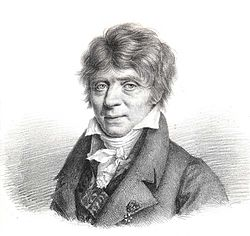
\includegraphics[width=2.0in]{Gaspard_de_Prony}
\end{figure}
\end{frame}
%--------------------------------------------------------------------------------------
\begin{frame}{Spectral Estimation}
	
	\begin{columns}
		
		\column{0.35\textwidth}
		\begin{figure}
			\centering
			\scalebox{0.60}{% This file was created by matlab2tikz.
%
%The latest updates can be retrieved from
%  http://www.mathworks.com/matlabcentral/fileexchange/22022-matlab2tikz-matlab2tikz
%where you can also make suggestions and rate matlab2tikz.
%
\definecolor{mycolor1}{rgb}{0.00000,0.44700,0.74100}%
%
\begin{tikzpicture}

\begin{axis}[%
width=2.521in,
height=0.866in,
at={(0.758in,2.626in)},
scale only axis,
xmin=0,
xmax=0.5,
xlabel style={font=\color{white!20!black}},
xlabel={ time (in secs)},
ymin=-1,
ymax=1,
axis background/.style={fill=white},
title style={font=\bfseries},
title={ Real part},
axis x line*=bottom,
axis y line*=left
]
\addplot [ycomb, color=mycolor1, mark=o, mark options={solid, mycolor1}, forget plot, line width=1.3pt]
  table[row sep=crcr]{%
0	1\\
0.0066666666666666	0.913545457642601\\
0.0133333333333334	0.669130606358858\\
0.02	0.309016994374947\\
0.0266666666666666	-0.104528463267654\\
0.0333333333333334	-0.5\\
0.04	-0.809016994374947\\
0.0466666666666666	-0.978147600733806\\
0.0533333333333332	-0.978147600733806\\
0.0600000000000001	-0.809016994374947\\
0.0666666666666667	-0.5\\
0.0733333333333333	-0.104528463267653\\
0.0800000000000001	0.309016994374947\\
0.0866666666666667	0.669130606358858\\
0.0933333333333333	0.913545457642601\\
0.1	1\\
0.106666666666667	0.913545457642601\\
0.113333333333333	0.669130606358858\\
0.12	0.309016994374947\\
0.126666666666667	-0.104528463267654\\
0.133333333333333	-0.499999999999999\\
0.14	-0.809016994374947\\
0.146666666666667	-0.978147600733806\\
0.153333333333333	-0.978147600733805\\
0.16	-0.809016994374948\\
0.166666666666667	-0.5\\
0.173333333333333	-0.104528463267653\\
0.18	0.309016994374949\\
0.186666666666667	0.669130606358858\\
0.193333333333333	0.913545457642601\\
0.2	1\\
0.206666666666667	0.9135454576426\\
0.213333333333333	0.669130606358858\\
0.22	0.309016994374948\\
0.226666666666667	-0.104528463267654\\
0.233333333333333	-0.499999999999999\\
0.24	-0.809016994374948\\
0.246666666666667	-0.978147600733806\\
0.253333333333333	-0.978147600733806\\
0.26	-0.809016994374948\\
0.266666666666667	-0.500000000000002\\
0.273333333333333	-0.104528463267656\\
0.28	0.309016994374947\\
0.286666666666667	0.669130606358857\\
0.293333333333333	0.913545457642601\\
0.3	1\\
0.306666666666667	0.913545457642602\\
0.313333333333333	0.669130606358858\\
0.32	0.309016994374948\\
0.326666666666667	-0.104528463267652\\
0.333333333333333	-0.5\\
0.34	-0.809016994374945\\
0.346666666666667	-0.978147600733806\\
0.353333333333333	-0.978147600733806\\
0.36	-0.809016994374948\\
0.366666666666667	-0.499999999999999\\
0.373333333333333	-0.104528463267653\\
0.38	0.309016994374947\\
0.386666666666667	0.669130606358857\\
0.393333333333333	0.9135454576426\\
0.4	1\\
0.406666666666667	0.9135454576426\\
0.413333333333333	0.669130606358858\\
0.42	0.309016994374945\\
0.426666666666667	-0.104528463267655\\
0.433333333333333	-0.5\\
0.44	-0.809016994374947\\
0.446666666666667	-0.978147600733805\\
0.453333333333333	-0.978147600733806\\
0.46	-0.809016994374948\\
0.466666666666667	-0.500000000000002\\
0.473333333333333	-0.104528463267654\\
0.48	0.30901699437495\\
0.486666666666667	0.669130606358859\\
0.493333333333333	0.913545457642601\\
};

\addplot[ycomb, color=red, mark=o, mark options={solid, red}, forget plot,line width=1.2pt] 
table[row sep=crcr] {%
0.166666666666667	-0.5\\
0.226666666666667	-0.104528463267654\\
};
\addplot[forget plot,, line width=1.3pt, color=white!15!black] table[row sep=crcr] {%
0	0\\
0.5	0\\
};
\end{axis}

\begin{axis}[%
width=2.521in,
height=0.866in,
at={(0.758in,0.553in)},
scale only axis,
xmin=0,
xmax=0.5,
xlabel style={font=\color{white!15!black}},
xlabel={ time (in secs)},
ymin=-1,
ymax=1,
axis background/.style={fill=white},
title style={font=\bfseries},
title={ Imag part},
axis x line*=bottom,
axis y line*=left
]
\addplot [ycomb, color=mycolor1, mark=o, mark options={solid, mycolor1}, forget plot, line width=1.2pt]
  table[row sep=crcr]{%
0	0\\
0.00666666666666671	0.4067366430758\\
0.0133333333333333	0.743144825477394\\
0.02	0.951056516295154\\
0.0266666666666666	0.994521895368273\\
0.0333333333333333	0.866025403784439\\
0.04	0.587785252292473\\
0.0466666666666666	0.207911690817759\\
0.0533333333333333	-0.20791169081776\\
0.0600000000000001	-0.587785252292473\\
0.0666666666666667	-0.866025403784438\\
0.0733333333333334	-0.994521895368273\\
0.08	-0.951056516295154\\
0.0866666666666667	-0.743144825477394\\
0.0933333333333334	-0.4067366430758\\
0.106666666666667	0.4067366430758\\
0.113333333333333	0.743144825477394\\
0.12	0.951056516295154\\
0.126666666666667	0.994521895368273\\
0.133333333333333	0.866025403784439\\
0.14	0.587785252292473\\
0.146666666666667	0.207911690817759\\
0.153333333333333	-0.20791169081776\\
0.16	-0.587785252292473\\
0.166666666666667	-0.866025403784439\\
0.173333333333333	-0.994521895368273\\
0.18	-0.951056516295153\\
0.186666666666667	-0.743144825477394\\
0.193333333333333	-0.4067366430758\\
0.206666666666667	0.406736643075802\\
0.213333333333333	0.743144825477395\\
0.22	0.951056516295153\\
0.226666666666667	0.994521895368273\\
0.233333333333333	0.866025403784439\\
0.24	0.587785252292472\\
0.246666666666667	0.207911690817759\\
0.253333333333333	-0.207911690817756\\
0.26	-0.587785252292473\\
0.266666666666667	-0.866025403784438\\
0.273333333333333	-0.994521895368273\\
0.28	-0.951056516295154\\
0.286666666666667	-0.743144825477395\\
0.293333333333333	-0.4067366430758\\
0.306666666666667	0.406736643075798\\
0.313333333333333	0.743144825477394\\
0.32	0.951056516295153\\
0.326666666666667	0.994521895368274\\
0.333333333333333	0.866025403784438\\
0.34	0.587785252292477\\
0.346666666666667	0.207911690817758\\
0.353333333333333	-0.20791169081776\\
0.36	-0.587785252292472\\
0.366666666666667	-0.866025403784439\\
0.373333333333333	-0.994521895368273\\
0.38	-0.951056516295154\\
0.386666666666667	-0.743144825477396\\
0.393333333333333	-0.406736643075803\\
0.406666666666667	0.406736643075801\\
0.413333333333333	0.743144825477394\\
0.42	0.951056516295154\\
0.426666666666667	0.994521895368273\\
0.433333333333333	0.866025403784439\\
0.44	0.587785252292474\\
0.446666666666667	0.207911690817762\\
0.453333333333333	-0.207911690817759\\
0.46	-0.587785252292472\\
0.466666666666667	-0.866025403784437\\
0.473333333333333	-0.994521895368273\\
0.48	-0.951056516295153\\
0.486666666666667	-0.743144825477393\\
0.493333333333333	-0.4067366430758\\
};
\addplot[ycomb, color=red, mark=o, mark options={solid, red}, forget plot, line width=1.2pt] table[row sep=crcr] {%
0.166666666666667	-0.866025403784439\\
0.226666666666667	0.994521895368273\\
};
\addplot[forget plot, line width=1.3pt, color=white!15!black] table[row sep=crcr] 
		\end{figure}
		
		\column{0.45\textwidth}
		\begin{figure}
			\centering
			\scalebox{0.60}{% This file was created by matlab2tikz.
%
%The latest updates can be retrieved from
%  http://www.mathworks.com/matlabcentral/fileexchange/22022-matlab2tikz-matlab2tikz
%where you can also make suggestions and rate matlab2tikz.
%
\definecolor{mycolor1}{rgb}{0.00000,0.44700,0.74100}%
%
\begin{tikzpicture}

\begin{axis}[%
width=2.521in,
height=1.566in,
at={(0.758in,0.481in)},
scale only axis,
xmin=-10,
xmax=80,
xlabel style={font=\color{white!18!black}},
xlabel={\large Frequency (in Hz)},
ymin=-0.2,
ymax=1.5,
ylabel style={font=\color{white!18!black} \huge},
ylabel={\large Amplitude},
axis background/.style={fill=white}
]
\addplot[ycomb, color=mycolor1, mark=o, mark options={solid, mycolor1}, forget plot, line width=1.5pt] table[row sep=crcr] {%
-1	-7.80856860653027e-17\\
1	5.54737013052344e-17\\
3	-1.33299290452969e-16\\
5	1.72199350464534e-16\\
7	-2.03706791656917e-16\\
9	1\\
11	2.12826963462994e-16\\
13	-1.88409144290174e-16\\
15	1.17298027143794e-16\\
17	-5.06183599878824e-17\\
19	1.2145450180656e-16\\
21	6.65590161214178e-18\\
23	-5.11169652285557e-17\\
25	-3.3980259771565e-16\\
27	-8.1650613803451e-17\\
29	8.1776737237564e-17\\
31	4.62075430080503e-17\\
33	-1.03796415855746e-16\\
35	-2.76611402488693e-17\\
37	-3.54863882138752e-17\\
39	5.4363639987515e-17\\
41	-4.57206624453587e-17\\
43	1.70695533926606e-17\\
45	5.01305772605862e-17\\
47	1.43448059713648e-16\\
49	8.23121093751715e-17\\
51	5.26806674147705e-17\\
53	-5.38444384061568e-18\\
55	3.76573585255343e-17\\
57	-4.74378843649705e-17\\
59	1.71682748802393e-17\\
61	1.42167711700981e-17\\
63	-7.24755132659825e-17\\
65	-1.90991577210353e-16\\
67	2.74758979639872e-16\\
69	3.22791812652835e-17\\
71	-2.66176168978996e-18\\
73	3.08512743180054e-17\\
};
\addplot[forget plot, color=white!15!black] table[row sep=crcr] 
		\end{figure}

        \begin{itemize}
        \item $N=75$
        \item $x[n] = A e^{j \frac{2 \pi {\color{blue}{k}} n}{N}}$, $\omega = e^{j \frac{2 \pi}{N}}$
        \pause
        \item $x[n_1] = A \omega^{{\color{red}{k}}n_1}$
        \item $x[n_1+1] = A \omega^k \ \omega^{{\color{red}{k}}n_1}$
		\end{itemize}
	\end{columns}	
\end{frame}
%--------------------------------------------------------------------------------------
\begin{frame}{Spectral Estimation}
	
        \begin{columns}		
		\column{0.35\textwidth}
		\begin{figure}
			\centering
			\scalebox{0.60}{% This file was created by matlab2tikz.
%
%The latest updates can be retrieved from
%  http://www.mathworks.com/matlabcentral/fileexchange/22022-matlab2tikz-matlab2tikz
%where you can also make suggestions and rate matlab2tikz.
%
\definecolor{mycolor1}{rgb}{0.00000,0.44700,0.74100}%
%
\begin{tikzpicture}

\begin{axis}[%
width=2.821in,
height=0.866in,
at={(0.758in,2.626in)},
scale only axis,
xmin=0,
xmax=0.5,
xlabel style={font=\color{white!15!black}},
xlabel={time (in secs)},
ymin=-5,
ymax=5,
axis background/.style={fill=white},
title style={font=\bfseries},
title={ Real part},
axis x line*=bottom,
axis y line*=left
]
\addplot [color=mycolor1, forget plot, line width=1.3pt]
  table[row sep=crcr]{%
0	5\\
0.00666666666666682	4.71262844706881\\
0.0133333333333336	3.89614455955154\\
0.0199999999999996	2.67966434321257\\
0.0333333333333332	-0.161738787282283\\
0.04	-1.35539739316685\\
0.0466666666666669	-2.15941162929721\\
0.0533333333333337	-2.47774106198011\\
0.0599999999999996	-2.30146994406622\\
0.0666666666666664	-1.70905692653531\\
0.0733333333333333	-0.851425031033491\\
0.0800000000000001	0.0754923999946966\\
0.0866666666666669	0.865964683707713\\
0.0933333333333337	1.34130969190107\\
0.0999999999999996	1.38196601125011\\
0.106666666666666	0.949212852448976\\
0.113333333333333	0.0927528240124404\\
0.12	-1.05717841950412\\
0.126666666666667	-2.31183105000068\\
0.133333333333334	-3.45629520146761\\
0.14	-4.28660395490134\\
0.146666666666667	-4.64517132252243\\
0.153333333333333	-4.44843291350493\\
0.16	-3.70189896262222\\
0.166666666666667	-2.5\\
0.173333333333334	-1.01072948444659\\
0.18	0.552288353953397\\
0.186666666666667	1.96550697930986\\
0.193333333333333	3.03280243005263\\
0.2	3.61803398874989\\
0.206666666666667	3.66722844316752\\
0.213333333333333	3.21659004880132\\
0.22	2.38498823796767\\
0.233333333333333	0.327090915285205\\
0.24	-0.489884660867582\\
0.246666666666667	-0.941457083702408\\
0.253333333333333	-0.94145708370241\\
0.26	-0.489884660867581\\
0.266666666666667	0.327090915285198\\
0.28	2.38498823796766\\
0.286666666666667	3.21659004880132\\
0.293333333333333	3.66722844316753\\
0.3	3.6180339887499\\
0.306666666666667	3.03280243005263\\
0.313333333333333	1.96550697930986\\
0.32	0.552288353953394\\
0.326666666666667	-1.01072948444658\\
0.333333333333333	-2.5\\
0.34	-3.70189896262221\\
0.346666666666667	-4.44843291350493\\
0.353333333333334	-4.64517132252243\\
0.36	-4.28660395490135\\
0.366666666666667	-3.45629520146761\\
0.373333333333333	-2.31183105000068\\
0.38	-1.05717841950412\\
0.386666666666667	0.0927528240124351\\
0.393333333333334	0.949212852448973\\
0.4	1.38196601125011\\
0.406666666666666	1.34130969190107\\
0.413333333333333	0.865964683707711\\
0.42	0.0754923999946904\\
0.426666666666667	-0.851425031033495\\
0.433333333333334	-1.70905692653531\\
0.44	-2.30146994406622\\
0.446666666666666	-2.47774106198011\\
0.453333333333333	-2.15941162929721\\
0.46	-1.35539739316685\\
0.466666666666667	-0.16173878728229\\
0.48	2.67966434321258\\
0.486666666666666	3.89614455955154\\
0.493333333333333	4.71262844706881\\
};
\addplot[ycomb, color=red, mark=o, mark options={solid, red}, forget plot, line width=1.pt] table[row sep=crcr] {%
0.18	0.552288353953397\\
0.24	-0.489884660867582\\
0.286666666666667	3.21659004880132\\
0.34	-3.70189896262221\\
};
\addplot[forget plot, color=white!15!black, line width=1.3pt] table[row sep=crcr] {%
0	0\\
0.5	0\\
};
\end{axis}

\begin{axis}[%
width=2.821in,
height=0.866in,
at={(0.758in,0.553in)},
scale only axis,
xmin=0,
xmax=0.5,
xlabel style={font=\color{white!15!black}},
xlabel={ time (in secs)},
ymin=-5,
ymax=5,
axis background/.style={fill=white},
title style={font=\bfseries},
title={ Imag part},
axis x line*=bottom,
axis y line*=left
]
\addplot [color=mycolor1, forget plot, line width=1.3pt]
  table[row sep=crcr]{%
0	0\\
0.00666666666666682	1.55374742265961\\
0.0133333333333336	2.88716776990935\\
0.0199999999999996	3.81667689708889\\
0.0266666666666664	4.22586124666144\\
0.0333333333333332	4.0843658623081\\
0.04	3.45201160788145\\
0.0466666666666669	2.46746137563028\\
0.0533333333333337	1.32342273329304\\
0.0599999999999996	0.232697699979123\\
0.0666666666666664	-0.609032420616769\\
0.0733333333333333	-1.0572405525095\\
0.0800000000000001	-1.04351544395342\\
0.0866666666666669	-0.587136058164774\\
0.0933333333333337	0.208735430038207\\
0.0999999999999996	1.17557050458495\\
0.106666666666666	2.10948028759726\\
0.113333333333333	2.80749807032113\\
0.12	3.10383601601407\\
0.126666666666667	2.89981437864642\\
0.133333333333334	2.1822528297178\\
0.14	1.02710665150806\\
0.146666666666667	-0.412318946292983\\
0.153333333333333	-1.93057628043349\\
0.16	-3.304382242429\\
0.166666666666667	-4.33012701892219\\
0.173333333333334	-4.8581296650886\\
0.18	-4.81774405034284\\
0.186666666666667	-4.22899584338187\\
0.193333333333333	-3.19875459515338\\
0.2	-1.90211303259031\\
0.206666666666667	-0.552197229235023\\
0.213333333333333	0.636374640383791\\
0.22	1.48407533702808\\
0.226666666666667	1.87678258761813\\
0.233333333333333	1.78460292520172\\
0.24	1.26597598254771\\
0.246666666666667	0.456379385788646\\
0.253333333333333	-0.45637938578864\\
0.26	-1.26597598254771\\
0.266666666666667	-1.78460292520171\\
0.273333333333333	-1.87678258761813\\
0.28	-1.48407533702808\\
0.286666666666667	-0.636374640383796\\
0.293333333333333	0.55219722923503\\
0.3	1.9021130325903\\
0.306666666666667	3.19875459515337\\
0.313333333333333	4.22899584338187\\
0.32	4.81774405034284\\
0.326666666666667	4.8581296650886\\
0.333333333333333	4.33012701892219\\
0.34	3.30438224242901\\
0.346666666666667	1.93057628043349\\
0.353333333333334	0.412318946292982\\
0.36	-1.02710665150806\\
0.366666666666667	-2.1822528297178\\
0.373333333333333	-2.89981437864642\\
0.38	-3.10383601601407\\
0.386666666666667	-2.80749807032113\\
0.393333333333334	-2.10948028759726\\
0.4	-1.17557050458495\\
0.406666666666666	-0.208735430038202\\
0.413333333333333	0.587136058164775\\
0.42	1.04351544395342\\
0.426666666666667	1.0572405525095\\
0.433333333333334	0.609032420616769\\
0.44	-0.232697699979121\\
0.446666666666666	-1.32342273329304\\
0.453333333333333	-2.46746137563028\\
0.46	-3.45201160788145\\
0.466666666666667	-4.0843658623081\\
0.473333333333334	-4.22586124666144\\
0.48	-3.81667689708889\\
0.486666666666666	-2.88716776990935\\
0.493333333333333	-1.55374742265961\\
};
\addplot[ycomb, color=red, mark=o, mark options={solid, red}, forget plot, line width=1.2pt] table[row sep=crcr] {%
0.18	-4.81774405034284\\
0.24	1.26597598254771\\
0.286666666666667	-0.636374640383796\\
0.34	3.30438224242901\\
};
\addplot[forget plot, color=white!15!black, line width=1.3pt] table[row sep=crcr] 
		\end{figure}
		
		\column{0.55\textwidth}
		\begin{figure}
			\centering
			\scalebox{0.60}{% This file was created by matlab2tikz.
%
%The latest updates can be retrieved from
%  http://www.mathworks.com/matlabcentral/fileexchange/22022-matlab2tikz-matlab2tikz
%where you can also make suggestions and rate matlab2tikz.
%
\definecolor{mycolor1}{rgb}{0.00000,0.44700,0.74100}%
%
\begin{tikzpicture}

\begin{axis}[%
width=2.521in,
height=1.566in,
at={(0.758in,0.481in)},
scale only axis,
xmin=-10,
xmax=80,
xlabel style={font=\color{white!15!black}},
xlabel={\large Frequency (in Hz)},
ymin=-0.5,
ymax=5,
ylabel style={font=\color{white!15!black}},
ylabel={\large Amplitude},
axis background/.style={fill=white}
]
\addplot[ycomb, color=mycolor1, mark=o, mark options={solid, mycolor1}, forget plot, line width=1.5pt] table[row sep=crcr] {%
-1	-1.71714494475358e-16\\
1	-3.32192326632562e-17\\
3	2\\
5	6.36756194043996e-16\\
7	-6.25200772111643e-16\\
9	3\\
11	6.07803629907803e-16\\
13	-4.10086171541976e-16\\
15	4.83533902924616e-16\\
17	-1.88743231204658e-16\\
19	1.37717742738638e-16\\
21	-5.94035344108608e-17\\
23	-8.94276053284954e-17\\
25	-8.55195277126423e-16\\
27	-2.87785699436618e-16\\
29	3.29917032992949e-16\\
31	1.13935019992171e-16\\
33	-2.05609274391086e-16\\
35	-2.1773379717422e-16\\
37	-1.0981336702209e-16\\
39	1.12627716491805e-17\\
41	-3.72817859003741e-17\\
43	1.07796053793514e-16\\
45	1.9349711122778e-16\\
47	5.84810875724067e-16\\
49	1.96021674545667e-16\\
51	2.37506161653534e-16\\
53	-6.08834920049603e-17\\
55	3.61933111657454e-16\\
57	-8.63052867720239e-17\\
59	-8.67258401635857e-17\\
61	2.54904711428452e-16\\
63	-2.77381552564259e-16\\
65	-6.55357268942932e-16\\
67	7.15686418621269e-16\\
69	6.96077568672224e-18\\
71	-7.82525462565175e-17\\
73	9.84049406607401e-17\\
};
\addplot[forget plot, color=white!15!black] table[row sep=crcr] 
		\end{figure}

        \begin{itemize}
        \item $x[n] = A_1 \omega^{k_1n} + A_2 \omega^{k_2 n}$
        \pause
        \item $x[n_1] = A_1 \omega^{k_1n_1} + A_2 \omega^{k_2 n_2}$
        \item $x[n_1+1] =  A_1 \omega^{k_1} \omega^{k_1n_1} + A_2 \omega^{k_2} \omega^{k_2 n_2}$
		\end{itemize}
	\end{columns}	
\pause
\begin{block}{Prony's method does not really work}
\begin{itemize}
  \item Not robust to noise
\end{itemize}
\end{block}
\end{frame}
%-----------------------------------------
\begin{frame}\frametitle{Sparse Fourier Transform Approach}
        \begin{block}{Robust Sparse Fourier Transform - Pawar and Ramchandran'14}
	 		\begin{itemize}
	 			\item[-] Sparse graph code approach
	 			\item[-] Computational complexity : $O(N \log N)$
	 		\end{itemize}
	 	\end{block}
\pause
\begin{block}{Key modifications}
   \begin{itemize}
   	\item Optimized for the induced noise model
   	\item Correlation peak is always {\color{blue} positive}
   	\item Take advantage in decoding algorithm - {\color{blue}sub-linear} time complexity
   \end{itemize}
\end{block}
\pause
        \begin{block}{Faster GPS receiver - Hassanieh '12}
	 		\begin{itemize}
	 			\item[-] Exploited sparsity in Correlation function $R_{XY}$
                \item[-] Algorithm based on hashing
                \item[-] In this application, complexity is still $O(N \log N)$
	 		\end{itemize}		
	 	\end{block}	 	


\end{frame}



%--------------------------------------------------------------------------------------
\def\fracty{0.45}
\def\fractx{0.8}
\begin{frame}{Example}
	%	\begin{figure}[t]
	%		\centering
	%		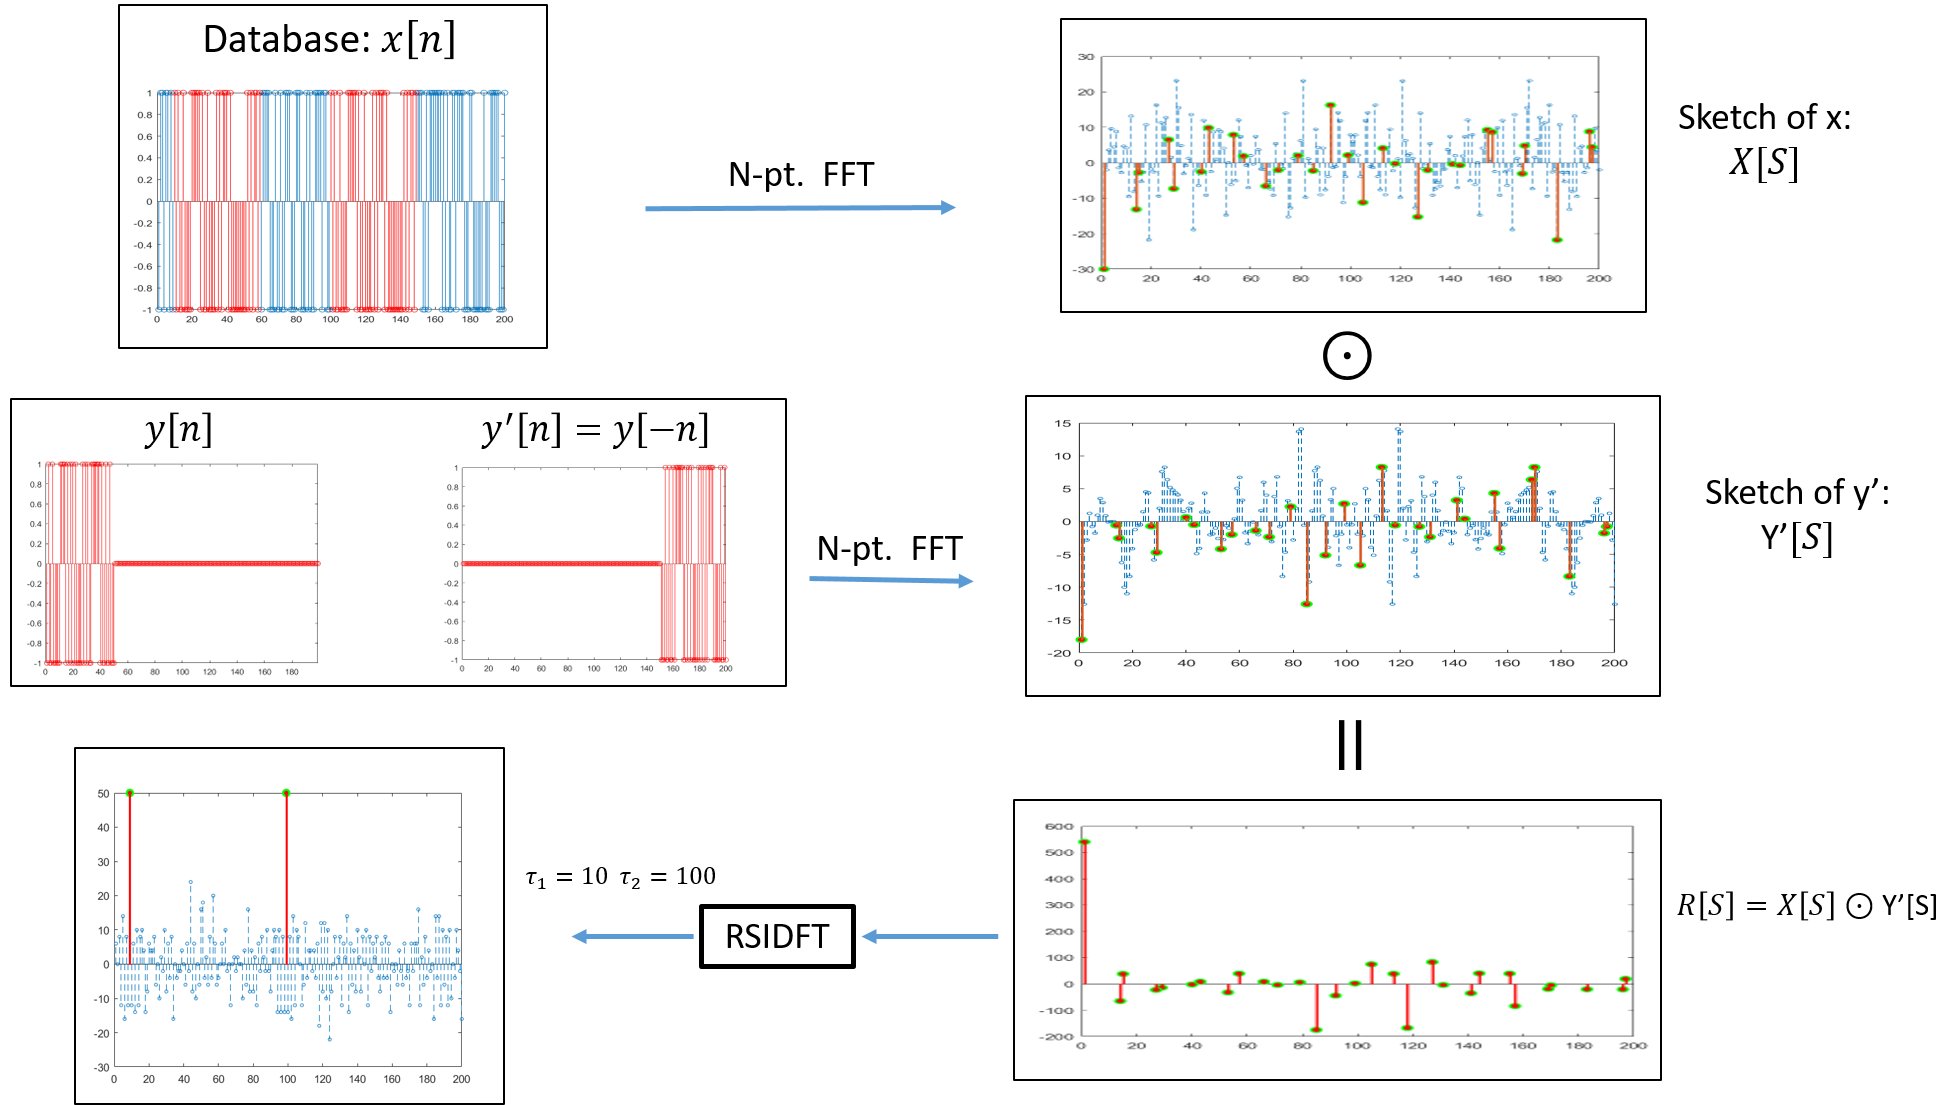
\includegraphics[width=4.8in]{Example_full_framework}
	%	\end{figure}
	
	\begin{figure}[t]
		\centering
		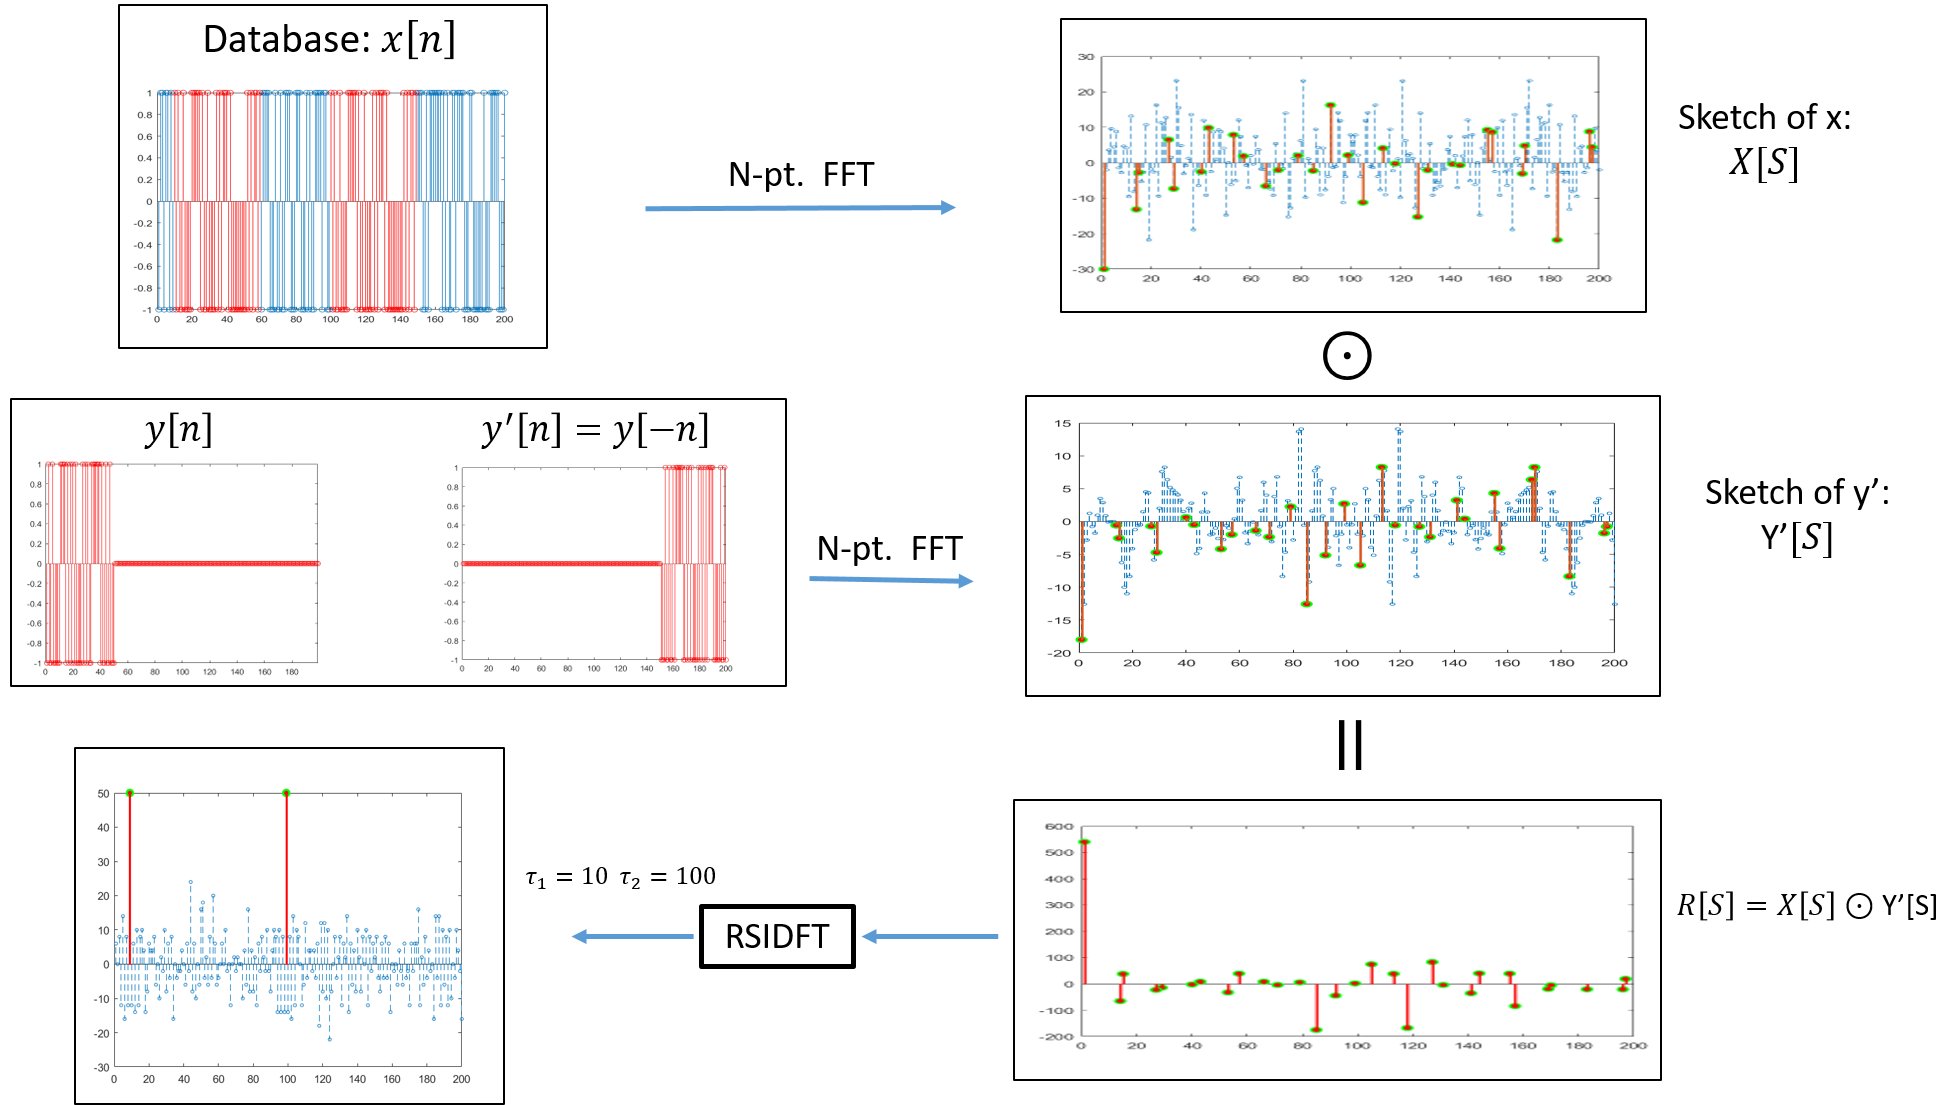
\includegraphics[width=4.8in]{Example_full_framework}
	\end{figure}
	
	%\begin{columns}
	%\vspace{-2.0in}
	%\begin{column}{0.48\textwidth}
	%%	Signal Domain
	%\begin{figure}
	%\centering
	%%\text{$x[n]:$}
	%%\resizebox{\fractx\columnwidth}{\fracty\columnwidth}{% This file was created by matlab2tikz v0.4.7 running on MATLAB 7.14.
% Copyright (c) 2008--2014, Nico Schlömer <nico.schloemer@gmail.com>
% All rights reserved.
% Minimal pgfplots version: 1.3
% 
% The latest updates can be retrieved from
%   http://www.mathworks.com/matlabcentral/fileexchange/22022-matlab2tikz
% where you can also make suggestions and rate matlab2tikz.
% 
%
% defining custom colors
\definecolor{mycolor1}{rgb}{0.00000,0.44700,0.74100}%
%
\begin{tikzpicture}
\pgfplotsset{every tick label/.append style={font=\Huge}}

\begin{axis}[%
width=6.01828521434821in,
height=4.74667979002625in,
scale only axis,
xmin=0,
xmax=200,
ymin=-1,
ymax=1,
xtick={0,50,...,150,200},
ytick={-1,0,1}
]

\addplot[ycomb,color=mycolor1,solid,mark=o,mark options={solid}] plot table[row sep=crcr] {1	-1\\
2	1\\
3	-1\\
4	1\\
5	-1\\
6	-1\\
7	-1\\
8	1\\
9	1\\
10	1\\
11	-1\\
12	1\\
13	1\\
14	1\\
15	-1\\
16	1\\
17	-1\\
18	-1\\
19	-1\\
20	1\\
21	1\\
22	-1\\
23	-1\\
24	1\\
25	-1\\
26	1\\
27	1\\
28	1\\
29	-1\\
30	-1\\
31	-1\\
32	1\\
33	-1\\
34	1\\
35	-1\\
36	1\\
37	-1\\
38	1\\
39	-1\\
40	1\\
41	-1\\
42	1\\
43	1\\
44	1\\
45	1\\
46	-1\\
47	1\\
48	1\\
49	1\\
50	-1\\
51	1\\
52	-1\\
53	-1\\
54	1\\
55	1\\
56	1\\
57	-1\\
58	1\\
59	-1\\
60	-1\\
61	1\\
62	1\\
63	1\\
64	-1\\
65	-1\\
66	-1\\
67	1\\
68	1\\
69	1\\
70	-1\\
71	-1\\
72	-1\\
73	-1\\
74	-1\\
75	1\\
76	-1\\
77	1\\
78	1\\
79	-1\\
80	1\\
81	1\\
82	-1\\
83	-1\\
84	1\\
85	-1\\
86	1\\
87	1\\
88	1\\
89	1\\
90	1\\
91	1\\
92	1\\
93	1\\
94	-1\\
95	1\\
96	1\\
97	1\\
98	-1\\
99	-1\\
100	1\\
101	-1\\
102	1\\
103	1\\
104	1\\
105	-1\\
106	1\\
107	-1\\
108	-1\\
109	-1\\
110	1\\
111	1\\
112	-1\\
113	-1\\
114	1\\
115	-1\\
116	1\\
117	1\\
118	1\\
119	-1\\
120	-1\\
121	-1\\
122	1\\
123	-1\\
124	1\\
125	-1\\
126	1\\
127	-1\\
128	1\\
129	-1\\
130	1\\
131	-1\\
132	1\\
133	1\\
134	1\\
135	1\\
136	-1\\
137	1\\
138	1\\
139	1\\
140	-1\\
141	1\\
142	-1\\
143	-1\\
144	1\\
145	1\\
146	1\\
147	-1\\
148	1\\
149	-1\\
150	1\\
151	1\\
152	1\\
153	-1\\
154	-1\\
155	1\\
156	-1\\
157	-1\\
158	-1\\
159	1\\
160	-1\\
161	1\\
162	-1\\
163	-1\\
164	-1\\
165	1\\
166	1\\
167	-1\\
168	1\\
169	1\\
170	-1\\
171	-1\\
172	-1\\
173	-1\\
174	1\\
175	1\\
176	1\\
177	-1\\
178	1\\
179	1\\
180	-1\\
181	-1\\
182	-1\\
183	1\\
184	1\\
185	1\\
186	-1\\
187	1\\
188	-1\\
189	1\\
190	1\\
191	1\\
192	1\\
193	-1\\
194	1\\
195	-1\\
196	-1\\
197	-1\\
198	-1\\
199	-1\\
200	1\\
};
\addplot [color=white!15!black,solid,forget plot]
  table[row sep=crcr]{0	0\\
200	0\\
};
\addplot[ycomb,color=red,solid,mark=o,mark options={solid}] plot table[row sep=crcr] {10	1\\
11	-1\\
12	1\\
13	1\\
14	1\\
15	-1\\
16	1\\
17	-1\\
18	-1\\
19	-1\\
20	1\\
21	1\\
22	-1\\
23	-1\\
24	1\\
25	-1\\
26	1\\
27	1\\
28	1\\
29	-1\\
30	-1\\
31	-1\\
32	1\\
33	-1\\
34	1\\
35	-1\\
36	1\\
37	-1\\
38	1\\
39	-1\\
40	1\\
41	-1\\
42	1\\
43	1\\
44	1\\
45	1\\
46	-1\\
47	1\\
48	1\\
49	1\\
50	-1\\
51	1\\
52	-1\\
53	-1\\
54	1\\
55	1\\
56	1\\
57	-1\\
58	1\\
59	-1\\
};
\addplot[ycomb,color=red,solid,mark=o,mark options={solid}] plot table[row sep=crcr] {100	1\\
101	-1\\
102	1\\
103	1\\
104	1\\
105	-1\\
106	1\\
107	-1\\
108	-1\\
109	-1\\
110	1\\
111	1\\
112	-1\\
113	-1\\
114	1\\
115	-1\\
116	1\\
117	1\\
118	1\\
119	-1\\
120	-1\\
121	-1\\
122	1\\
123	-1\\
124	1\\
125	-1\\
126	1\\
127	-1\\
128	1\\
129	-1\\
130	1\\
131	-1\\
132	1\\
133	1\\
134	1\\
135	1\\
136	-1\\
137	1\\
138	1\\
139	1\\
140	-1\\
141	1\\
142	-1\\
143	-1\\
144	1\\
145	1\\
146	1\\
147	-1\\
148	1\\
149	-1\\
};
\end{axis}
\end{tikzpicture}%}
	%% This file was created by matlab2tikz v0.4.7 running on MATLAB 7.14.
% Copyright (c) 2008--2014, Nico Schlömer <nico.schloemer@gmail.com>
% All rights reserved.
% Minimal pgfplots version: 1.3
% 
% The latest updates can be retrieved from
%   http://www.mathworks.com/matlabcentral/fileexchange/22022-matlab2tikz
% where you can also make suggestions and rate matlab2tikz.
% 
%
% defining custom colors
\definecolor{mycolor1}{rgb}{0.00000,0.44700,0.74100}%
%
\begin{tikzpicture}
\pgfplotsset{every tick label/.append style={font=\Huge}}

\begin{axis}[%
width=6.01828521434821in,
height=4.74667979002625in,
scale only axis,
xmin=0,
xmax=200,
ymin=-1,
ymax=1,
xtick={0,50,...,150,200},
ytick={-1,0,1}
]

\addplot[ycomb,color=mycolor1,solid,mark=o,mark options={solid}] plot table[row sep=crcr] {1	-1\\
2	1\\
3	-1\\
4	1\\
5	-1\\
6	-1\\
7	-1\\
8	1\\
9	1\\
10	1\\
11	-1\\
12	1\\
13	1\\
14	1\\
15	-1\\
16	1\\
17	-1\\
18	-1\\
19	-1\\
20	1\\
21	1\\
22	-1\\
23	-1\\
24	1\\
25	-1\\
26	1\\
27	1\\
28	1\\
29	-1\\
30	-1\\
31	-1\\
32	1\\
33	-1\\
34	1\\
35	-1\\
36	1\\
37	-1\\
38	1\\
39	-1\\
40	1\\
41	-1\\
42	1\\
43	1\\
44	1\\
45	1\\
46	-1\\
47	1\\
48	1\\
49	1\\
50	-1\\
51	1\\
52	-1\\
53	-1\\
54	1\\
55	1\\
56	1\\
57	-1\\
58	1\\
59	-1\\
60	-1\\
61	1\\
62	1\\
63	1\\
64	-1\\
65	-1\\
66	-1\\
67	1\\
68	1\\
69	1\\
70	-1\\
71	-1\\
72	-1\\
73	-1\\
74	-1\\
75	1\\
76	-1\\
77	1\\
78	1\\
79	-1\\
80	1\\
81	1\\
82	-1\\
83	-1\\
84	1\\
85	-1\\
86	1\\
87	1\\
88	1\\
89	1\\
90	1\\
91	1\\
92	1\\
93	1\\
94	-1\\
95	1\\
96	1\\
97	1\\
98	-1\\
99	-1\\
100	1\\
101	-1\\
102	1\\
103	1\\
104	1\\
105	-1\\
106	1\\
107	-1\\
108	-1\\
109	-1\\
110	1\\
111	1\\
112	-1\\
113	-1\\
114	1\\
115	-1\\
116	1\\
117	1\\
118	1\\
119	-1\\
120	-1\\
121	-1\\
122	1\\
123	-1\\
124	1\\
125	-1\\
126	1\\
127	-1\\
128	1\\
129	-1\\
130	1\\
131	-1\\
132	1\\
133	1\\
134	1\\
135	1\\
136	-1\\
137	1\\
138	1\\
139	1\\
140	-1\\
141	1\\
142	-1\\
143	-1\\
144	1\\
145	1\\
146	1\\
147	-1\\
148	1\\
149	-1\\
150	1\\
151	1\\
152	1\\
153	-1\\
154	-1\\
155	1\\
156	-1\\
157	-1\\
158	-1\\
159	1\\
160	-1\\
161	1\\
162	-1\\
163	-1\\
164	-1\\
165	1\\
166	1\\
167	-1\\
168	1\\
169	1\\
170	-1\\
171	-1\\
172	-1\\
173	-1\\
174	1\\
175	1\\
176	1\\
177	-1\\
178	1\\
179	1\\
180	-1\\
181	-1\\
182	-1\\
183	1\\
184	1\\
185	1\\
186	-1\\
187	1\\
188	-1\\
189	1\\
190	1\\
191	1\\
192	1\\
193	-1\\
194	1\\
195	-1\\
196	-1\\
197	-1\\
198	-1\\
199	-1\\
200	1\\
};
\addplot [color=white!15!black,solid,forget plot]
  table[row sep=crcr]{0	0\\
200	0\\
};
\addplot[ycomb,color=red,solid,mark=o,mark options={solid}] plot table[row sep=crcr] {10	1\\
11	-1\\
12	1\\
13	1\\
14	1\\
15	-1\\
16	1\\
17	-1\\
18	-1\\
19	-1\\
20	1\\
21	1\\
22	-1\\
23	-1\\
24	1\\
25	-1\\
26	1\\
27	1\\
28	1\\
29	-1\\
30	-1\\
31	-1\\
32	1\\
33	-1\\
34	1\\
35	-1\\
36	1\\
37	-1\\
38	1\\
39	-1\\
40	1\\
41	-1\\
42	1\\
43	1\\
44	1\\
45	1\\
46	-1\\
47	1\\
48	1\\
49	1\\
50	-1\\
51	1\\
52	-1\\
53	-1\\
54	1\\
55	1\\
56	1\\
57	-1\\
58	1\\
59	-1\\
};
\addplot[ycomb,color=red,solid,mark=o,mark options={solid}] plot table[row sep=crcr] {100	1\\
101	-1\\
102	1\\
103	1\\
104	1\\
105	-1\\
106	1\\
107	-1\\
108	-1\\
109	-1\\
110	1\\
111	1\\
112	-1\\
113	-1\\
114	1\\
115	-1\\
116	1\\
117	1\\
118	1\\
119	-1\\
120	-1\\
121	-1\\
122	1\\
123	-1\\
124	1\\
125	-1\\
126	1\\
127	-1\\
128	1\\
129	-1\\
130	1\\
131	-1\\
132	1\\
133	1\\
134	1\\
135	1\\
136	-1\\
137	1\\
138	1\\
139	1\\
140	-1\\
141	1\\
142	-1\\
143	-1\\
144	1\\
145	1\\
146	1\\
147	-1\\
148	1\\
149	-1\\
};
\end{axis}
\end{tikzpicture}%
	%\end{figure}
	%\vspace{-0.2in}
	%
	%\begin{figure}
	%\centering
	%%\resizebox{\fractx\columnwidth}{\fracty\columnwidth}{% This file was created by matlab2tikz v0.4.7 running on MATLAB 7.14.
% Copyright (c) 2008--2014, Nico Schlömer <nico.schloemer@gmail.com>
% All rights reserved.
% Minimal pgfplots version: 1.3
% 
% The latest updates can be retrieved from
%   http://www.mathworks.com/matlabcentral/fileexchange/22022-matlab2tikz
% where you can also make suggestions and rate matlab2tikz.
% 
\begin{tikzpicture}
\pgfplotsset{every tick label/.append style={font=\Huge}}

\begin{axis}[%
width=10in,
height=8in,
scale only axis,
xmin=0,
xmax=199,
ymin=-1,
ymax=1,xtick={0,50,...,150,200},
ytick={-1,0,1},
clip=false
]
\node at (axis cs:-25,0) {\Huge{$y[n]$}};
\addplot[ycomb,color=red,solid,mark=o,mark options={solid}] plot table[row sep=crcr] {1	1\\
2	-1\\
3	1\\
4	1\\
5	1\\
6	-1\\
7	1\\
8	-1\\
9	-1\\
10	-1\\
11	1\\
12	1\\
13	-1\\
14	-1\\
15	1\\
16	-1\\
17	1\\
18	1\\
19	1\\
20	-1\\
21	-1\\
22	-1\\
23	1\\
24	-1\\
25	1\\
26	-1\\
27	1\\
28	-1\\
29	1\\
30	-1\\
31	1\\
32	-1\\
33	1\\
34	1\\
35	1\\
36	1\\
37	-1\\
38	1\\
39	1\\
40	1\\
41	-1\\
42	1\\
43	-1\\
44	-1\\
45	1\\
46	1\\
47	1\\
48	-1\\
49	1\\
50	-1\\
51	0\\
52	0\\
53	0\\
54	0\\
55	0\\
56	0\\
57	0\\
58	0\\
59	0\\
60	0\\
61	0\\
62	0\\
63	0\\
64	0\\
65	0\\
66	0\\
67	0\\
68	0\\
69	0\\
70	0\\
71	0\\
72	0\\
73	0\\
74	0\\
75	0\\
76	0\\
77	0\\
78	0\\
79	0\\
80	0\\
81	0\\
82	0\\
83	0\\
84	0\\
85	0\\
86	0\\
87	0\\
88	0\\
89	0\\
90	0\\
91	0\\
92	0\\
93	0\\
94	0\\
95	0\\
96	0\\
97	0\\
98	0\\
99	0\\
100	0\\
101	0\\
102	0\\
103	0\\
104	0\\
105	0\\
106	0\\
107	0\\
108	0\\
109	0\\
110	0\\
111	0\\
112	0\\
113	0\\
114	0\\
115	0\\
116	0\\
117	0\\
118	0\\
119	0\\
120	0\\
121	0\\
122	0\\
123	0\\
124	0\\
125	0\\
126	0\\
127	0\\
128	0\\
129	0\\
130	0\\
131	0\\
132	0\\
133	0\\
134	0\\
135	0\\
136	0\\
137	0\\
138	0\\
139	0\\
140	0\\
141	0\\
142	0\\
143	0\\
144	0\\
145	0\\
146	0\\
147	0\\
148	0\\
149	0\\
150	0\\
151	0\\
152	0\\
153	0\\
154	0\\
155	0\\
156	0\\
157	0\\
158	0\\
159	0\\
160	0\\
161	0\\
162	0\\
163	0\\
164	0\\
165	0\\
166	0\\
167	0\\
168	0\\
169	0\\
170	0\\
171	0\\
172	0\\
173	0\\
174	0\\
175	0\\
176	0\\
177	0\\
178	0\\
179	0\\
180	0\\
181	0\\
182	0\\
183	0\\
184	0\\
185	0\\
186	0\\
187	0\\
188	0\\
189	0\\
190	0\\
191	0\\
192	0\\
193	0\\
194	0\\
195	0\\
196	0\\
197	0\\
198	0\\
199	0\\
200	0\\
};
\addplot [color=white!15!black,solid,forget plot]
  table[row sep=crcr]{0	0\\
199	0\\
};
\end{axis}
\end{tikzpicture}%}
	%% This file was created by matlab2tikz v0.4.7 running on MATLAB 7.14.
% Copyright (c) 2008--2014, Nico Schlömer <nico.schloemer@gmail.com>
% All rights reserved.
% Minimal pgfplots version: 1.3
% 
% The latest updates can be retrieved from
%   http://www.mathworks.com/matlabcentral/fileexchange/22022-matlab2tikz
% where you can also make suggestions and rate matlab2tikz.
% 
\begin{tikzpicture}
\pgfplotsset{every tick label/.append style={font=\Huge}}

\begin{axis}[%
width=10in,
height=8in,
scale only axis,
xmin=0,
xmax=199,
ymin=-1,
ymax=1,xtick={0,50,...,150,200},
ytick={-1,0,1},
clip=false
]
\node at (axis cs:-25,0) {\Huge{$y[n]$}};
\addplot[ycomb,color=red,solid,mark=o,mark options={solid}] plot table[row sep=crcr] {1	1\\
2	-1\\
3	1\\
4	1\\
5	1\\
6	-1\\
7	1\\
8	-1\\
9	-1\\
10	-1\\
11	1\\
12	1\\
13	-1\\
14	-1\\
15	1\\
16	-1\\
17	1\\
18	1\\
19	1\\
20	-1\\
21	-1\\
22	-1\\
23	1\\
24	-1\\
25	1\\
26	-1\\
27	1\\
28	-1\\
29	1\\
30	-1\\
31	1\\
32	-1\\
33	1\\
34	1\\
35	1\\
36	1\\
37	-1\\
38	1\\
39	1\\
40	1\\
41	-1\\
42	1\\
43	-1\\
44	-1\\
45	1\\
46	1\\
47	1\\
48	-1\\
49	1\\
50	-1\\
51	0\\
52	0\\
53	0\\
54	0\\
55	0\\
56	0\\
57	0\\
58	0\\
59	0\\
60	0\\
61	0\\
62	0\\
63	0\\
64	0\\
65	0\\
66	0\\
67	0\\
68	0\\
69	0\\
70	0\\
71	0\\
72	0\\
73	0\\
74	0\\
75	0\\
76	0\\
77	0\\
78	0\\
79	0\\
80	0\\
81	0\\
82	0\\
83	0\\
84	0\\
85	0\\
86	0\\
87	0\\
88	0\\
89	0\\
90	0\\
91	0\\
92	0\\
93	0\\
94	0\\
95	0\\
96	0\\
97	0\\
98	0\\
99	0\\
100	0\\
101	0\\
102	0\\
103	0\\
104	0\\
105	0\\
106	0\\
107	0\\
108	0\\
109	0\\
110	0\\
111	0\\
112	0\\
113	0\\
114	0\\
115	0\\
116	0\\
117	0\\
118	0\\
119	0\\
120	0\\
121	0\\
122	0\\
123	0\\
124	0\\
125	0\\
126	0\\
127	0\\
128	0\\
129	0\\
130	0\\
131	0\\
132	0\\
133	0\\
134	0\\
135	0\\
136	0\\
137	0\\
138	0\\
139	0\\
140	0\\
141	0\\
142	0\\
143	0\\
144	0\\
145	0\\
146	0\\
147	0\\
148	0\\
149	0\\
150	0\\
151	0\\
152	0\\
153	0\\
154	0\\
155	0\\
156	0\\
157	0\\
158	0\\
159	0\\
160	0\\
161	0\\
162	0\\
163	0\\
164	0\\
165	0\\
166	0\\
167	0\\
168	0\\
169	0\\
170	0\\
171	0\\
172	0\\
173	0\\
174	0\\
175	0\\
176	0\\
177	0\\
178	0\\
179	0\\
180	0\\
181	0\\
182	0\\
183	0\\
184	0\\
185	0\\
186	0\\
187	0\\
188	0\\
189	0\\
190	0\\
191	0\\
192	0\\
193	0\\
194	0\\
195	0\\
196	0\\
197	0\\
198	0\\
199	0\\
200	0\\
};
\addplot [color=white!15!black,solid,forget plot]
  table[row sep=crcr]{0	0\\
199	0\\
};
\end{axis}
\end{tikzpicture}%
	%\end{figure}
	%
	%\vspace{-0.2in}
	%
	%\begin{figure}
	%\centering
	%%\resizebox{\fractx\columnwidth}{\fracty\columnwidth}{% This file was created by matlab2tikz.
%
%The latest updates can be retrieved from
%  http://www.mathworks.com/matlabcentral/fileexchange/22022-matlab2tikz-matlab2tikz
%where you can also make suggestions and rate matlab2tikz.
%
\definecolor{mycolor1}{rgb}{0.00000,0.44700,0.74100}%
%
\begin{tikzpicture}
\pgfplotsset{every tick label/.append style={font=\Huge}}

\begin{axis}[%
width=4.521in,
height=3.566in,
at={(0.758in,0.481in)},
scale only axis,
xmin=0,
xmax=200,
ymin=-30,
ymax=50,
axis background/.style={fill=white},
xtick={0,50,...,150,200},
ytick={-50,0,50}
]
\addplot[ycomb, color=mycolor1, dashed, mark size=1.5pt, mark=o, mark options={solid, mycolor1}, forget plot] table[row sep=crcr] {%
1	6\\
2	-2.27373675443232e-15\\
3	8\\
4	-12\\
5	14\\
6	-16\\
7	8\\
8	-12\\
9	50\\
10	-12\\
11	6\\
12	-14\\
13	10\\
14	-12\\
15	8\\
16	10\\
17	4\\
18	-14\\
19	-8\\
20	6\\
21	4\\
22	4\\
23	8\\
24	-6\\
25	4.54747350886464e-15\\
26	-10\\
27	2\\
28	-2\\
29	10\\
30	-8\\
31	6\\
32	-4\\
33	8\\
34	-16\\
35	-5.6843418860808e-15\\
36	-4\\
37	-2\\
38	-2\\
39	4\\
40	4.54747350886464e-15\\
41	-6\\
42	6\\
43	-2\\
44	24\\
45	-8\\
46	6\\
47	-10\\
48	-1.98951966012828e-15\\
49	-6\\
50	16\\
51	18\\
52	-4\\
53	2\\
54	-6\\
55	8\\
56	-4\\
57	20\\
58	6\\
59	-6\\
60	-4\\
61	-1.27897692436818e-15\\
62	6\\
63	-1.13686837721616e-15\\
64	10\\
65	-2\\
66	-3.41060513164848e-15\\
67	-12\\
68	1.4210854715202e-15\\
69	2\\
70	-2\\
71	2\\
72	-5.6843418860808e-16\\
73	8.5265128291212e-16\\
74	-10\\
75	4\\
76	-6\\
77	16\\
78	-8\\
79	4\\
80	-8\\
81	2\\
82	-12\\
83	6\\
84	-2\\
85	8.00000000000001\\
86	2\\
87	-2\\
88	10\\
89	-2\\
90	-8\\
91	4\\
92	10\\
93	8\\
94	-14\\
95	9.99999999999999\\
96	-14\\
97	8\\
98	-14\\
99	50\\
100	-14\\
101	8\\
102	-16\\
103	14\\
104	-12\\
105	10\\
106	8\\
107	-1.13686837721616e-15\\
108	-12\\
109	-5.99999999999999\\
110	12\\
111	-4\\
112	4\\
113	4\\
114	-2.00000000000001\\
115	4\\
116	-4\\
117	6\\
118	-18\\
119	12\\
120	-7.99999999999999\\
121	12\\
122	-10\\
123	10\\
124	-22\\
125	-8.00000000000001\\
126	5.6843418860808e-16\\
127	8.00000000000001\\
128	-4\\
129	2\\
130	8\\
131	-12\\
132	6\\
133	2\\
134	14\\
135	-14\\
136	6\\
137	-6\\
138	4\\
139	-8.00000000000001\\
140	10\\
141	2\\
142	-8\\
143	8\\
144	-1.70530256582424e-15\\
145	10\\
146	-12\\
147	8\\
148	-2\\
149	5.99999999999999\\
150	2\\
151	8\\
152	-4\\
153	-8\\
154	6\\
155	-4\\
156	8\\
157	-4\\
158	6\\
159	-14\\
160	-3.41060513164848e-15\\
161	-2\\
162	3.41060513164848e-15\\
163	-6\\
164	4\\
165	-2\\
166	-6\\
167	5.99999999999999\\
168	-4\\
169	-2\\
170	-12\\
171	6\\
172	-2\\
173	6\\
174	6\\
175	16\\
176	-12\\
177	2\\
178	-6\\
179	8\\
180	-3.99999999999999\\
181	4\\
182	-2\\
183	-1.13686837721616e-15\\
184	-16\\
185	14\\
186	-4\\
187	14\\
188	-12\\
189	9.99999999999999\\
190	-6\\
191	8\\
192	-12\\
193	10\\
194	-10\\
195	3.97903932025656e-15\\
196	-4\\
197	10\\
198	4\\
199	-1.99999999999999\\
200	-16\\
};
\addplot[forget plot, color=white!15!black, dashed] table[row sep=crcr] {%
0	0\\
200	0\\
};
\addplot[ycomb, color=red, line width=2.0pt, mark=*, mark options={solid, fill=red, green}, forget plot] table[row sep=crcr] {%
9	50\\
};
\addplot[forget plot, color=white!15!black, line width=2.0pt] table[row sep=crcr] {%
0	0\\
200	0\\
};
\addplot[ycomb, color=red, line width=2.0pt, mark=*, mark options={solid, fill=red, green}, forget plot] table[row sep=crcr] {%
99	50\\
};
\addplot[forget plot, color=white!15!black, line width=2.0pt] table[row sep=crcr] 
	%% This file was created by matlab2tikz.
%
%The latest updates can be retrieved from
%  http://www.mathworks.com/matlabcentral/fileexchange/22022-matlab2tikz-matlab2tikz
%where you can also make suggestions and rate matlab2tikz.
%
\definecolor{mycolor1}{rgb}{0.00000,0.44700,0.74100}%
%
\begin{tikzpicture}
\pgfplotsset{every tick label/.append style={font=\Huge}}

\begin{axis}[%
width=4.521in,
height=3.566in,
at={(0.758in,0.481in)},
scale only axis,
xmin=0,
xmax=200,
ymin=-30,
ymax=50,
axis background/.style={fill=white},
xtick={0,50,...,150,200},
ytick={-50,0,50}
]
\addplot[ycomb, color=mycolor1, dashed, mark size=1.5pt, mark=o, mark options={solid, mycolor1}, forget plot] table[row sep=crcr] {%
1	6\\
2	-2.27373675443232e-15\\
3	8\\
4	-12\\
5	14\\
6	-16\\
7	8\\
8	-12\\
9	50\\
10	-12\\
11	6\\
12	-14\\
13	10\\
14	-12\\
15	8\\
16	10\\
17	4\\
18	-14\\
19	-8\\
20	6\\
21	4\\
22	4\\
23	8\\
24	-6\\
25	4.54747350886464e-15\\
26	-10\\
27	2\\
28	-2\\
29	10\\
30	-8\\
31	6\\
32	-4\\
33	8\\
34	-16\\
35	-5.6843418860808e-15\\
36	-4\\
37	-2\\
38	-2\\
39	4\\
40	4.54747350886464e-15\\
41	-6\\
42	6\\
43	-2\\
44	24\\
45	-8\\
46	6\\
47	-10\\
48	-1.98951966012828e-15\\
49	-6\\
50	16\\
51	18\\
52	-4\\
53	2\\
54	-6\\
55	8\\
56	-4\\
57	20\\
58	6\\
59	-6\\
60	-4\\
61	-1.27897692436818e-15\\
62	6\\
63	-1.13686837721616e-15\\
64	10\\
65	-2\\
66	-3.41060513164848e-15\\
67	-12\\
68	1.4210854715202e-15\\
69	2\\
70	-2\\
71	2\\
72	-5.6843418860808e-16\\
73	8.5265128291212e-16\\
74	-10\\
75	4\\
76	-6\\
77	16\\
78	-8\\
79	4\\
80	-8\\
81	2\\
82	-12\\
83	6\\
84	-2\\
85	8.00000000000001\\
86	2\\
87	-2\\
88	10\\
89	-2\\
90	-8\\
91	4\\
92	10\\
93	8\\
94	-14\\
95	9.99999999999999\\
96	-14\\
97	8\\
98	-14\\
99	50\\
100	-14\\
101	8\\
102	-16\\
103	14\\
104	-12\\
105	10\\
106	8\\
107	-1.13686837721616e-15\\
108	-12\\
109	-5.99999999999999\\
110	12\\
111	-4\\
112	4\\
113	4\\
114	-2.00000000000001\\
115	4\\
116	-4\\
117	6\\
118	-18\\
119	12\\
120	-7.99999999999999\\
121	12\\
122	-10\\
123	10\\
124	-22\\
125	-8.00000000000001\\
126	5.6843418860808e-16\\
127	8.00000000000001\\
128	-4\\
129	2\\
130	8\\
131	-12\\
132	6\\
133	2\\
134	14\\
135	-14\\
136	6\\
137	-6\\
138	4\\
139	-8.00000000000001\\
140	10\\
141	2\\
142	-8\\
143	8\\
144	-1.70530256582424e-15\\
145	10\\
146	-12\\
147	8\\
148	-2\\
149	5.99999999999999\\
150	2\\
151	8\\
152	-4\\
153	-8\\
154	6\\
155	-4\\
156	8\\
157	-4\\
158	6\\
159	-14\\
160	-3.41060513164848e-15\\
161	-2\\
162	3.41060513164848e-15\\
163	-6\\
164	4\\
165	-2\\
166	-6\\
167	5.99999999999999\\
168	-4\\
169	-2\\
170	-12\\
171	6\\
172	-2\\
173	6\\
174	6\\
175	16\\
176	-12\\
177	2\\
178	-6\\
179	8\\
180	-3.99999999999999\\
181	4\\
182	-2\\
183	-1.13686837721616e-15\\
184	-16\\
185	14\\
186	-4\\
187	14\\
188	-12\\
189	9.99999999999999\\
190	-6\\
191	8\\
192	-12\\
193	10\\
194	-10\\
195	3.97903932025656e-15\\
196	-4\\
197	10\\
198	4\\
199	-1.99999999999999\\
200	-16\\
};
\addplot[forget plot, color=white!15!black, dashed] table[row sep=crcr] {%
0	0\\
200	0\\
};
\addplot[ycomb, color=red, line width=2.0pt, mark=*, mark options={solid, fill=red, green}, forget plot] table[row sep=crcr] {%
9	50\\
};
\addplot[forget plot, color=white!15!black, line width=2.0pt] table[row sep=crcr] {%
0	0\\
200	0\\
};
\addplot[ycomb, color=red, line width=2.0pt, mark=*, mark options={solid, fill=red, green}, forget plot] table[row sep=crcr] {%
99	50\\
};
\addplot[forget plot, color=white!15!black, line width=2.0pt] table[row sep=crcr] {%
0	0\\
200	0\\
};
\end{axis}
\end{tikzpicture}%
	%\end{figure}
	%\end{column}
	%
	%%\begin{column}{0.48\textwidth}
	%%\tiny{Fourier Domain ($N$-pt FFT)}
	%%\begin{figure}
	%%\centering
	%%\resizebox{0.7\columnwidth}{!}{% This file was created by matlab2tikz.
%
%The latest updates can be retrieved from
%  http://www.mathworks.com/matlabcentral/fileexchange/22022-matlab2tikz-matlab2tikz
%where you can also make suggestions and rate matlab2tikz.
%
\definecolor{mycolor1}{rgb}{0.00000,0.44700,0.74100}%
\definecolor{mycolor2}{rgb}{0.85000,0.32500,0.09800}%
%
\begin{tikzpicture}

\begin{axis}[%
width=4.521in,
height=3.566in,
at={(0.758in,0.481in)},
scale only axis,
xmin=0,
xmax=200,
ymin=-40,
ymax=30,
axis background/.style={fill=white}
]
\addplot[ycomb, color=mycolor1, dashed, mark size=1.5pt, mark=o, mark options={solid, mycolor1}, forget plot] table[row sep=crcr] {%
1	16\\
2	-8.9408351634566\\
3	-0.201570148939315\\
4	-2.19729324165034\\
5	4.61376282934002\\
6	-9.8207773631622\\
7	-10.4413133825018\\
8	-1.76560342434666\\
9	-12.7342122520018\\
10	0.239212200768665\\
11	-10.069966513515\\
12	-8.00259742834581\\
13	-3.7016119897477\\
14	-6.92962190558934\\
15	-2.07137098362405\\
16	6.21473811307536\\
17	15.509315924071\\
18	1.51858780569097\\
19	21.034785215086\\
20	3.2110551163066\\
21	-7.18033988749895\\
22	7.16343375094051\\
23	-0.459471560598043\\
24	17.6234986651139\\
25	19.4801775025947\\
26	3.07106781186548\\
27	3.050228518555\\
28	-12.9225936854977\\
29	-13.7529289967405\\
30	16.3505513756278\\
31	5.64114196716989\\
32	-3.48150007701741\\
33	0.675456948063186\\
34	18.8626722543494\\
35	-17.5851623038878\\
36	-3.26118979097373\\
37	7.78740113585339\\
38	-11.3071731224103\\
39	8.9816779960111\\
40	2.68004446307097\\
41	-3.47213595499958\\
42	-22.0808434042411\\
43	-4.61906792769598\\
44	-6.04989252404458\\
45	6.99042158159403\\
46	2.63031430981386\\
47	0.604042111776057\\
48	-7.7139524995846\\
49	3.82718922865676\\
50	-9.70220137767649\\
51	-2\\
52	10.244863594685\\
53	4.04901270012725\\
54	21.5967083325753\\
55	-12.3629632832443\\
56	10.5997189357379\\
57	2.11556188302871\\
58	7.62252750891169\\
59	-21.0762975196776\\
60	-10.3265863542471\\
61	15.1803398874989\\
62	7.18171388316369\\
63	-2.15930492086648\\
64	10.2852483833618\\
65	-6.72865478166775\\
66	-1.86199739955865\\
67	-8.27469288490878\\
68	2.37590739317321\\
69	5.3227759658929\\
70	-6.33636332330854\\
71	6.53919792032906\\
72	2.58571417702316\\
73	-8.05439690327551\\
74	10.7173024051698\\
75	-13.0495167654792\\
76	-11.0710678118655\\
77	-6.35872255705589\\
78	-12.0621625943584\\
79	-3.53274299634243\\
80	-1.27873115694023\\
81	5.47213595499958\\
82	1.37798660693131\\
83	-8.57010451260969\\
84	-3.30066085985855\\
85	-3.76235315848312\\
86	-2.61941496754341\\
87	-5.21895471035773\\
88	22.6845647386842\\
89	-4.16488674019002\\
90	-12.3124434911097\\
91	-0.110373373983914\\
92	23.2555547877574\\
93	-16.1877575107804\\
94	-18.9693386755851\\
95	-7.01097609132525\\
96	-13.8813918373891\\
97	5.07444919072072\\
98	2.29195482089335\\
99	-17.0372238493697\\
100	-4.18870795493004\\
101	-36\\
102	-4.18870795493004\\
103	-17.0372238493697\\
104	2.29195482089335\\
105	5.07444919072072\\
106	-13.8813918373891\\
107	-7.01097609132525\\
108	-18.9693386755851\\
109	-16.1877575107804\\
110	23.2555547877574\\
111	-0.110373373983914\\
112	-12.3124434911097\\
113	-4.16488674019002\\
114	22.6845647386842\\
115	-5.21895471035773\\
116	-2.61941496754341\\
117	-3.76235315848312\\
118	-3.30066085985855\\
119	-8.57010451260969\\
120	1.37798660693131\\
121	5.47213595499958\\
122	-1.27873115694023\\
123	-3.53274299634243\\
124	-12.0621625943584\\
125	-6.35872255705589\\
126	-11.0710678118655\\
127	-13.0495167654792\\
128	10.7173024051698\\
129	-8.05439690327551\\
130	2.58571417702316\\
131	6.53919792032906\\
132	-6.33636332330854\\
133	5.3227759658929\\
134	2.37590739317321\\
135	-8.27469288490878\\
136	-1.86199739955865\\
137	-6.72865478166775\\
138	10.2852483833618\\
139	-2.15930492086648\\
140	7.18171388316369\\
141	15.1803398874989\\
142	-10.3265863542471\\
143	-21.0762975196776\\
144	7.62252750891169\\
145	2.11556188302871\\
146	10.5997189357379\\
147	-12.3629632832443\\
148	21.5967083325753\\
149	4.04901270012725\\
150	10.244863594685\\
151	-2\\
152	-9.70220137767649\\
153	3.82718922865676\\
154	-7.7139524995846\\
155	0.604042111776057\\
156	2.63031430981386\\
157	6.99042158159403\\
158	-6.04989252404458\\
159	-4.61906792769598\\
160	-22.0808434042411\\
161	-3.47213595499958\\
162	2.68004446307097\\
163	8.9816779960111\\
164	-11.3071731224103\\
165	7.78740113585339\\
166	-3.26118979097373\\
167	-17.5851623038878\\
168	18.8626722543494\\
169	0.675456948063186\\
170	-3.48150007701741\\
171	5.64114196716989\\
172	16.3505513756278\\
173	-13.7529289967405\\
174	-12.9225936854977\\
175	3.050228518555\\
176	3.07106781186548\\
177	19.4801775025947\\
178	17.6234986651139\\
179	-0.459471560598043\\
180	7.16343375094051\\
181	-7.18033988749895\\
182	3.2110551163066\\
183	21.034785215086\\
184	1.51858780569097\\
185	15.509315924071\\
186	6.21473811307536\\
187	-2.07137098362405\\
188	-6.92962190558934\\
189	-3.7016119897477\\
190	-8.00259742834581\\
191	-10.069966513515\\
192	0.239212200768665\\
193	-12.7342122520018\\
194	-1.76560342434666\\
195	-10.4413133825018\\
196	-9.8207773631622\\
197	4.61376282934002\\
198	-2.19729324165034\\
199	-0.201570148939315\\
200	-8.9408351634566\\
};
\addplot[forget plot, color=white!15!black, dashed] table[row sep=crcr] {%
0	0\\
200	0\\
};
\addplot[ycomb, color=mycolor2, line width=1.5pt, mark=*, mark options={solid, fill=red, green}, forget plot] table[row sep=crcr] {%
1	16\\
15	-2.07137098362405\\
29	-13.7529289967405\\
43	-4.61906792769598\\
57	2.11556188302871\\
71	6.53919792032906\\
85	-3.76235315848312\\
99	-17.0372238493697\\
113	-4.16488674019002\\
127	-13.0495167654792\\
141	15.1803398874989\\
155	0.604042111776057\\
169	0.675456948063186\\
183	21.034785215086\\
197	4.61376282934002\\
1	16\\
14	-6.92962190558934\\
27	3.050228518555\\
40	2.68004446307097\\
53	4.04901270012725\\
66	-1.86199739955865\\
79	-3.53274299634243\\
92	23.2555547877574\\
105	5.07444919072072\\
118	-3.30066085985855\\
131	6.53919792032906\\
144	7.62252750891169\\
157	6.99042158159403\\
170	-3.48150007701741\\
183	21.034785215086\\
196	-9.8207773631622\\
};
\addplot[forget plot, color=white!15!black, line width=1.5pt] table[row sep=crcr] 
	%%\end{figure}
	%%
	%%\begin{figure}
	%%\centering
	%%\resizebox{0.7\columnwidth}{!}{% This file was created by matlab2tikz.
%
%The latest updates can be retrieved from
%  http://www.mathworks.com/matlabcentral/fileexchange/22022-matlab2tikz-matlab2tikz
%where you can also make suggestions and rate matlab2tikz.
%
\definecolor{mycolor1}{rgb}{0.00000,0.44700,0.74100}%
\definecolor{mycolor2}{rgb}{0.85000,0.32500,0.09800}%
%
\begin{tikzpicture}

\begin{axis}[%
width=4.521in,
height=3.566in,
at={(0.758in,0.481in)},
scale only axis,
xmin=0,
xmax=200,
ymin=-20,
ymax=15,
axis background/.style={fill=white}
]
\addplot[ycomb, color=mycolor1, dashed, mark size=1.5pt, mark=o, mark options={solid, mycolor1}, forget plot] table[row sep=crcr] {%
1	6\\
2	2.83271699636813\\
3	-2.55331600456052\\
4	-3.12739150907618\\
5	1.97071747764893\\
6	6.44172485656756\\
7	5.15860337633778\\
8	0.417069999431173\\
9	-1.98264397420117\\
10	-0.177084558225608\\
11	3.15838444032454\\
12	5.41583294678269\\
13	5.66380848601647\\
14	3.43894144134494\\
15	-0.121639691403174\\
16	-1.55986247075773\\
17	0.324327310136643\\
18	1.18166295795646\\
19	-2.62619530099509\\
20	-6.85598328349429\\
21	-5\\
22	0.839325427411033\\
23	2.70675901473284\\
24	-0.445870410385353\\
25	-2.03320103483967\\
26	-0.464466094067262\\
27	-2.05563554855059\\
28	-8.30123783064314\\
29	-10.7995393475819\\
30	-4.63341574741165\\
31	2.49047455050557\\
32	2.16249670762443\\
33	-1.28251058658359\\
34	1.52762510907959\\
35	9.13103803433945\\
36	11.2498565186136\\
37	4.56155192930778\\
38	-3.00501522045944\\
39	-4.21149148356791\\
40	-0.999239975010603\\
41	1\\
42	0.477665531307964\\
43	-0.252336419180771\\
44	-0.200074706997802\\
45	-0.307707328937143\\
46	-0.649607440887396\\
47	-0.206509501507032\\
48	0.56496021380372\\
49	-0.274755875860278\\
50	-2.22090509065107\\
51	-1\\
52	5.54331162510844\\
53	12.0148229815972\\
54	11.1648247974624\\
55	4.80255816600299\\
56	2.22078289454225\\
57	5.93839504536803\\
58	7.18474725649803\\
59	0.299500881725923\\
60	-6.86916523861174\\
61	-5\\
62	1.46404716350854\\
63	1.70763012655204\\
64	-3.79213462058552\\
65	-5.05844826966984\\
66	0.28091207457242\\
67	4.03923161373666\\
68	1.77692573632648\\
69	-1.34409048264781\\
70	-0.796673607259429\\
71	1.03738949449485\\
72	1.08238600456105\\
73	-0.208064422484939\\
74	-2.4844093856037\\
75	-5.93428018481587\\
76	-7.53553390593274\\
77	-4.2861111069367\\
78	0.294255222840381\\
79	0.732927869736908\\
80	-0.894758552295153\\
81	1\\
82	4.37054021044068\\
83	3.19404609382282\\
84	-0.152140627756733\\
85	1.1517189726666\\
86	4.02909387757175\\
87	-0.058681780604843\\
88	-7.14741785081009\\
89	-4.34219508461949\\
90	6.87847859409933\\
91	9.31375151467504\\
92	-2.86600918875193\\
93	-13.6251715811334\\
94	-9.58999487041817\\
95	1.4256554039636\\
96	5.98709968977758\\
97	3.91909689275431\\
98	0.694674297992945\\
99	-5.17786466576518\\
100	-14.7535659655008\\
101	-20\\
102	-14.7535659655008\\
103	-5.17786466576518\\
104	0.694674297992945\\
105	3.91909689275431\\
106	5.98709968977758\\
107	1.4256554039636\\
108	-9.58999487041817\\
109	-13.6251715811334\\
110	-2.86600918875193\\
111	9.31375151467504\\
112	6.87847859409933\\
113	-4.34219508461949\\
114	-7.14741785081009\\
115	-0.058681780604843\\
116	4.02909387757175\\
117	1.1517189726666\\
118	-0.152140627756733\\
119	3.19404609382282\\
120	4.37054021044068\\
121	1\\
122	-0.894758552295153\\
123	0.732927869736908\\
124	0.294255222840381\\
125	-4.2861111069367\\
126	-7.53553390593274\\
127	-5.93428018481587\\
128	-2.4844093856037\\
129	-0.208064422484939\\
130	1.08238600456105\\
131	1.03738949449485\\
132	-0.796673607259429\\
133	-1.34409048264781\\
134	1.77692573632648\\
135	4.03923161373666\\
136	0.28091207457242\\
137	-5.05844826966984\\
138	-3.79213462058552\\
139	1.70763012655204\\
140	1.46404716350854\\
141	-5\\
142	-6.86916523861174\\
143	0.299500881725923\\
144	7.18474725649803\\
145	5.93839504536803\\
146	2.22078289454225\\
147	4.80255816600299\\
148	11.1648247974624\\
149	12.0148229815972\\
150	5.54331162510844\\
151	-1\\
152	-2.22090509065107\\
153	-0.274755875860278\\
154	0.56496021380372\\
155	-0.206509501507032\\
156	-0.649607440887396\\
157	-0.307707328937143\\
158	-0.200074706997802\\
159	-0.252336419180771\\
160	0.477665531307964\\
161	1\\
162	-0.999239975010603\\
163	-4.21149148356791\\
164	-3.00501522045944\\
165	4.56155192930778\\
166	11.2498565186136\\
167	9.13103803433945\\
168	1.52762510907959\\
169	-1.28251058658359\\
170	2.16249670762443\\
171	2.49047455050557\\
172	-4.63341574741165\\
173	-10.7995393475819\\
174	-8.30123783064314\\
175	-2.05563554855059\\
176	-0.464466094067262\\
177	-2.03320103483967\\
178	-0.445870410385353\\
179	2.70675901473284\\
180	0.839325427411033\\
181	-5\\
182	-6.85598328349429\\
183	-2.62619530099509\\
184	1.18166295795646\\
185	0.324327310136643\\
186	-1.55986247075773\\
187	-0.121639691403174\\
188	3.43894144134494\\
189	5.66380848601647\\
190	5.41583294678269\\
191	3.15838444032454\\
192	-0.177084558225608\\
193	-1.98264397420117\\
194	0.417069999431173\\
195	5.15860337633778\\
196	6.44172485656756\\
197	1.97071747764893\\
198	-3.12739150907618\\
199	-2.55331600456052\\
200	2.83271699636813\\
};
\addplot[forget plot, color=white!15!black, dashed] table[row sep=crcr] {%
0	0\\
200	0\\
};
\addplot[ycomb, color=mycolor2, line width=1.5pt, mark=*, mark options={solid, fill=red, green}, forget plot] table[row sep=crcr] {%
1	6\\
15	-0.121639691403174\\
29	-10.7995393475819\\
43	-0.252336419180771\\
57	5.93839504536803\\
71	1.03738949449485\\
85	1.1517189726666\\
99	-5.17786466576518\\
113	-4.34219508461949\\
127	-5.93428018481587\\
141	-5\\
155	-0.206509501507032\\
169	-1.28251058658359\\
183	-2.62619530099509\\
197	1.97071747764893\\
1	6\\
14	3.43894144134494\\
27	-2.05563554855059\\
40	-0.999239975010603\\
53	12.0148229815972\\
66	0.28091207457242\\
79	0.732927869736908\\
92	-2.86600918875193\\
105	3.91909689275431\\
118	-0.152140627756733\\
131	1.03738949449485\\
144	7.18474725649803\\
157	-0.307707328937143\\
170	2.16249670762443\\
183	-2.62619530099509\\
196	6.44172485656756\\
};
\addplot[forget plot, color=white!15!black, line width=1.5pt] table[row sep=crcr] 
	%%\end{figure}
	%%
	%%\begin{figure}
	%%\centering
	%%\resizebox{0.7\columnwidth}{!}{% This file was created by matlab2tikz.
%
%The latest updates can be retrieved from
%  http://www.mathworks.com/matlabcentral/fileexchange/22022-matlab2tikz-matlab2tikz
%where you can also make suggestions and rate matlab2tikz.
%
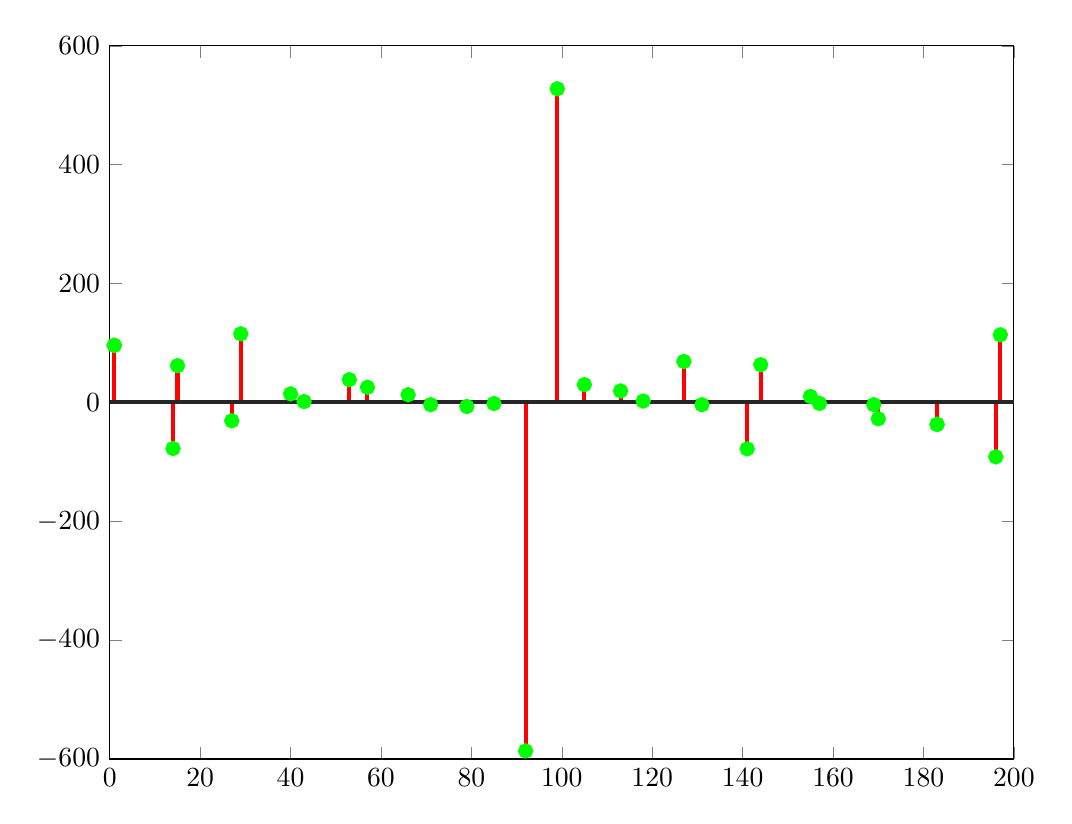
\begin{tikzpicture}

\begin{axis}[%
width=4.521in,
height=3.566in,
at={(0.758in,0.481in)},
scale only axis,
xmin=0,
xmax=200,
ymin=-600,
ymax=600,
axis background/.style={fill=white}
]
\addplot[ycomb, color=red, line width=1.5pt, mark=*, mark options={solid, fill=red, green}, forget plot] table[row sep=crcr] {%
1	96\\
15	61.8405159676837\\
29	115.396461869287\\
43	1.39320614430019\\
57	25.4543162795665\\
71	-3.824409687939\\
85	-1.90254204745981\\
99	527.693372169007\\
113	19.3349778052062\\
127	68.938951416754\\
141	-78.1377674149945\\
155	9.99707529364864\\
169	-3.75059930092979\\
183	-36.9748518197181\\
197	113.813269618881\\
1	96\\
14	-77.5471454188034\\
27	-30.9232662713007\\
40	14.3497108293358\\
53	38.2537557025721\\
66	12.8778537782972\\
79	-6.8710448873182\\
92	-586.390764014078\\
105	29.9833721024771\\
118	2.33185767595022\\
131	-3.824409687939\\
144	63.507357731341\\
157	-1.71860486624029\\
170	-27.5315139371526\\
183	-36.9748518197181\\
196	-91.5921246182205\\
};
\addplot[forget plot, color=white!15!black, line width=1.5pt] table[row sep=crcr] 
	%%\end{figure}
	%%\end{column}
	%
	%\end{columns}
\end{frame}
%---------------------------------------------------------
\begin{frame}\frametitle{Sparse Fourier Transform Approach}
	\begin{figure}[t]
		\centering
		\scalebox{0.28}{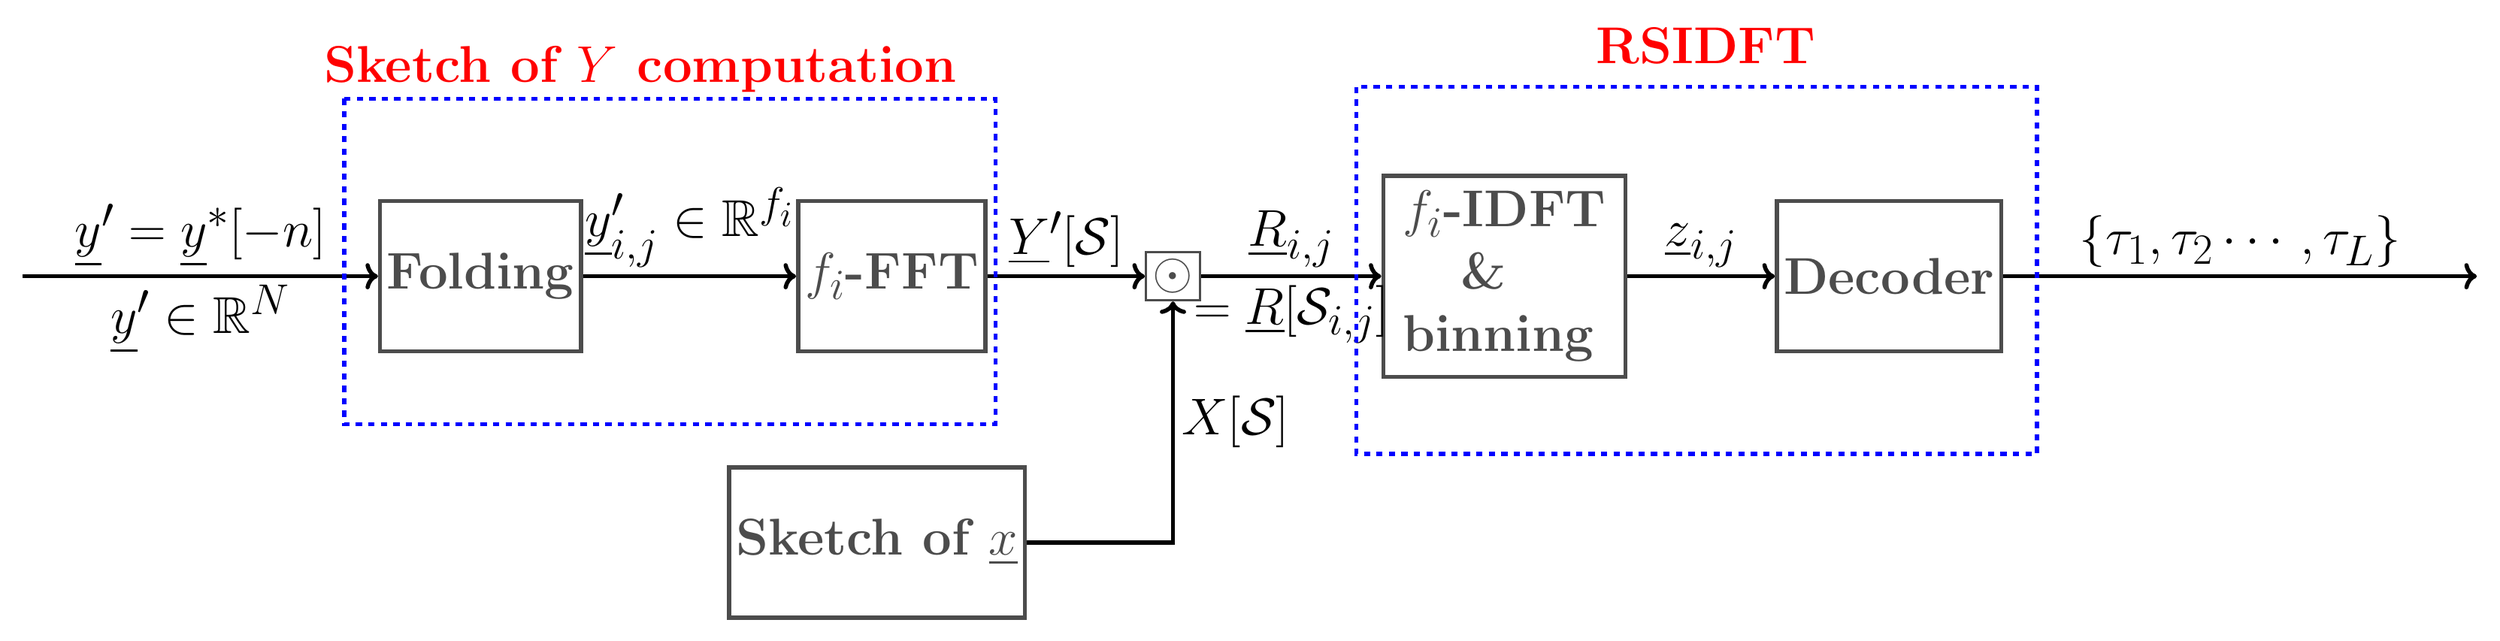
\begin{tikzpicture}

\def\nodewidth{1in}
\def\fsize{\Huge}
\tikzstyle{block} = [rectangle, draw, thick,opacity=0.7,line width =2, minimum size=\nodewidth]
\tikzstyle{opnode} = [rectangle, draw, thick,opacity=0.7,line width=1, minimum size=0.2in]

\node[block] (r1) at (-8.7,3){\fsize \bf Folding};
\node[block] (r2) at (-1.75,3) {\fsize \bf $f_i$-FFT};
\node[opnode] (r3) at (3,3) {\fsize \bf $\odot$};
\node[block,align=center] (r4) at (8.6,3) {\fsize \bf \begin{tabular}{l}
$f_i$-IDFT \\ 
~~ \& \\ 
binning
\end{tabular}};
\node[block] (r5) at (15.1,3) {\fsize \bf Decoder};
\node[block] (r6) at (-2,-1.5) {\fsize \bf Sketch of $\xv$};


\draw[<-, thick, line width=2] (r1.west)--node[midway, above]{\fsize $\yv'=\yv^*[-n]$}
node[midway, below]{\fsize $\yv'\in\mathbb{R}^N$}+(-6,0);
\draw[->, thick, line width=2] (r1.east)--node[midway, above]{\fsize $\yv'_{i,j}\in\mathbb{R}^{f_i}$}(r2.west);
\draw[->, thick, line width=2] (r2.east)--node[midway, above]{\fsize $\Yv'[\mc{S}]$}(r3.west);
\draw[->, thick, line width=2] (r3.east)--node[midway, above]{\fsize $\Rv_{i,j}$}
node[midway,below]{\fsize \bf $=\Rv[\mathcal{S}_{i,j}]$}(r4.west);
\draw[->, thick, line width=2] (r4.east)--node[midway, above]{\fsize $\zv_{i,j}$}(r5.west);
\draw[->, thick, line width=2] (r5.east)--node[midway, above]{\fsize $\{\tau_1, \tau_2 \cdots, \tau_L \}$}+(8,0);
\draw[->, thick, line width=2] let \p1=(r6),\p2= (r3) in (r6.east)--(\x2,\y1)--node[midway, right]{\fsize \bf $X[\mathcal{S}]$}  (r3.south);



\draw [dashed, line width =2, color=blue] (-11,6) rectangle (0,0.5);
\node[color= red] at (-6,6.5) {\fsize \bf  Sketch of $Y$ computation};
\draw [dashed, line width =2, color=blue]  (6.1,6.2) rectangle (17.6,0);
\node [color = red] at (12,6.9) {\fsize \bf RSIDFT};
\end{tikzpicture}}
	\end{figure}
\vspace{-0.2cm}
	 	\begin{block}{}
	 		\begin{equation}\label{eqn:Rxy_fourier}\nonumber
	 		\boxed{\rv = \underset{\text{\color{red} 3 } } {\mathcal{F}_{N}^{-1}} \ \{ \underset{\text{ \color{red} 1 } }{  \mathcal{F}_{N}\{\xv\}}  \odot \ \underset{\text{ \color{red} 2 } }{ \mathcal{F}_{N}\{\yv'\}}  \} }
	 		\end{equation}
	 		
	 		\begin{itemize}
	 			\item[\color{red} 1.] \textit{\color{blue} Sketch of $\xv$ : }  Assume $ \Xv[l] = \mathcal{F}\{\xv\}$ is precomputed at positions $l \in \mathcal{S}$.
	 			
	 			\item[\color{red} 2.] \textit{\color{blue} Sketch of $\yv$:}  Compute $ \Yv'[l] = \mathcal{F}\{\yv'\}$ for $l \in \mathcal{S}$.
	 			\begin{itemize}
	 				\item[-] Only $M$ non-zero values in $\yv'$ - Efficient computation (folding and adding)
	 			\end{itemize}
	 			
	 			\item[\color{red} 3.] \textit{\color{blue} Sparse $\mathcal{F}^{-1}$}:
	 			\begin{itemize}
	 				\item[-] Robust Sparse Inverse Fourier Transform (RSIDFT)
	 				\item[-] Efficient Implementation- {\color{blue} sublinear} time and sampling complexity
	 			\end{itemize}
	 		\end{itemize}
	 	\end{block}
\end{frame}


%%------------------------------------------------------------------
%\begin{frame}{Robust Sparse Inverse Fourier Transform(RSIDFT)}
%\begin{block}{Main Idea}
%	\begin{itemize}
%		\item \alert{Sub-sampling} in frequency corresponds to \alert{aliasing} in time
%		\item Aliased coefficients $\Leftrightarrow$ parity check constraints of \alert{GLDPC codes}
%		\item \alert{CRT} guided sub-sampling induces a code good for \alert{Peeling decoder}
%		\item R-FFAST- proposed by Pawar and Ramchandran 2014
%	\end{itemize}
%\end{block}
%\begin{block}{Key modifications}
%   \begin{itemize}
%   	\item Optimized for the induced noise model
%   	\item Correlation peak is always {\color{blue} positive}
%   	\item Take advantage in decoding algorithm - {\color{blue}sub-linear} time complexity
%   \end{itemize}
%\end{block}
%\end{frame}

%--------------------------------------------------------------------------------------
	\begin{frame}{DSP - A Quick Review}
			\begin{columns}
				
				\column{0.35\textwidth}
				\begin{figure}
					\centering
					\scalebox{0.60}{% This file was created by matlab2tikz.
%
%The latest updates can be retrieved from
%  http://www.mathworks.com/matlabcentral/fileexchange/22022-matlab2tikz-matlab2tikz
%where you can also make suggestions and rate matlab2tikz.
%
\definecolor{mycolor1}{rgb}{0.00000,0.44700,0.74100}%
%
\begin{tikzpicture}

\begin{axis}[%
width=2.821in,
height=0.866in,
at={(0.758in,2.626in)},
scale only axis,
xmin=0,
xmax=0.5,
xlabel style={font=\color{white!15!black}},
xlabel={time (in secs)},
ymin=-5,
ymax=5,
axis background/.style={fill=white},
title style={font=\bfseries},
title={ Time domain},
axis x line*=bottom,
axis y line*=left
]
\addplot [ycomb, color=mycolor1, mark=o, mark options={solid, mycolor1}, forget plot, line width=1.5pt]
  table[row sep=crcr]{%
0	5\\
0.00666666666666682	4.71262844706881\\
0.0133333333333336	3.89614455955154\\
0.0199999999999996	2.67966434321257\\
0.0333333333333332	-0.161738787282283\\
0.04	-1.35539739316685\\
0.0466666666666669	-2.15941162929721\\
0.0533333333333337	-2.47774106198011\\
0.0599999999999996	-2.30146994406622\\
0.0666666666666664	-1.70905692653531\\
0.0733333333333333	-0.851425031033491\\
0.0800000000000001	0.0754923999946966\\
0.0866666666666669	0.865964683707713\\
0.0933333333333337	1.34130969190107\\
0.0999999999999996	1.38196601125011\\
0.106666666666666	0.949212852448976\\
0.113333333333333	0.0927528240124404\\
0.12	-1.05717841950412\\
0.126666666666667	-2.31183105000068\\
0.133333333333334	-3.45629520146761\\
0.14	-4.28660395490134\\
0.146666666666667	-4.64517132252243\\
0.153333333333333	-4.44843291350493\\
0.16	-3.70189896262222\\
0.166666666666667	-2.5\\
0.173333333333334	-1.01072948444659\\
0.18	0.552288353953397\\
0.186666666666667	1.96550697930986\\
0.193333333333333	3.03280243005263\\
0.2	3.61803398874989\\
0.206666666666667	3.66722844316752\\
0.213333333333333	3.21659004880132\\
0.22	2.38498823796767\\
0.233333333333333	0.327090915285205\\
0.24	-0.489884660867582\\
0.246666666666667	-0.941457083702408\\
0.253333333333333	-0.94145708370241\\
0.26	-0.489884660867581\\
0.266666666666667	0.327090915285198\\
0.28	2.38498823796766\\
0.286666666666667	3.21659004880132\\
0.293333333333333	3.66722844316753\\
0.3	3.6180339887499\\
0.306666666666667	3.03280243005263\\
0.313333333333333	1.96550697930986\\
0.32	0.552288353953394\\
0.326666666666667	-1.01072948444658\\
0.333333333333333	-2.5\\
0.34	-3.70189896262221\\
0.346666666666667	-4.44843291350493\\
0.353333333333334	-4.64517132252243\\
0.36	-4.28660395490135\\
0.366666666666667	-3.45629520146761\\
0.373333333333333	-2.31183105000068\\
0.38	-1.05717841950412\\
0.386666666666667	0.0927528240124351\\
0.393333333333334	0.949212852448973\\
0.4	1.38196601125011\\
0.406666666666666	1.34130969190107\\
0.413333333333333	0.865964683707711\\
0.42	0.0754923999946904\\
0.426666666666667	-0.851425031033495\\
0.433333333333334	-1.70905692653531\\
0.44	-2.30146994406622\\
0.446666666666666	-2.47774106198011\\
0.453333333333333	-2.15941162929721\\
0.46	-1.35539739316685\\
0.466666666666667	-0.16173878728229\\
0.48	2.67966434321258\\
0.486666666666666	3.89614455955154\\
0.493333333333333	4.71262844706881\\
};
\end{axis}

\end{tikzpicture}%}
				\end{figure}
				
				\column{0.45\textwidth}
				\begin{figure}
					\centering
					\scalebox{0.60}{% This file was created by matlab2tikz.
%
%The latest updates can be retrieved from
%  http://www.mathworks.com/matlabcentral/fileexchange/22022-matlab2tikz-matlab2tikz
%where you can also make suggestions and rate matlab2tikz.
%
\definecolor{mycolor1}{rgb}{0.00000,0.44700,0.74100}%
%
\begin{tikzpicture}

\begin{axis}[%
width=2.521in,
height=1.566in,
at={(0.758in,0.481in)},
scale only axis,
xmin=-10,
xmax=80,
xlabel style={font=\color{white!15!black}},
xlabel={\large Frequency (in Hz)},
ymin=-0.5,
ymax=5,
ylabel style={font=\color{white!15!black}},
ylabel={\large Amplitude},
axis background/.style={fill=white}
]
\addplot[ycomb, color=mycolor1, mark=o, mark options={solid, mycolor1}, forget plot, line width=1.5pt] table[row sep=crcr] {%
-1	-1.71714494475358e-16\\
1	-3.32192326632562e-17\\
3	2\\
5	6.36756194043996e-16\\
7	-6.25200772111643e-16\\
9	3\\
11	6.07803629907803e-16\\
13	-4.10086171541976e-16\\
15	4.83533902924616e-16\\
17	-1.88743231204658e-16\\
19	1.37717742738638e-16\\
21	-5.94035344108608e-17\\
23	-8.94276053284954e-17\\
25	-8.55195277126423e-16\\
27	-2.87785699436618e-16\\
29	3.29917032992949e-16\\
31	1.13935019992171e-16\\
33	-2.05609274391086e-16\\
35	-2.1773379717422e-16\\
37	-1.0981336702209e-16\\
39	1.12627716491805e-17\\
41	-3.72817859003741e-17\\
43	1.07796053793514e-16\\
45	1.9349711122778e-16\\
47	5.84810875724067e-16\\
49	1.96021674545667e-16\\
51	2.37506161653534e-16\\
53	-6.08834920049603e-17\\
55	3.61933111657454e-16\\
57	-8.63052867720239e-17\\
59	-8.67258401635857e-17\\
61	2.54904711428452e-16\\
63	-2.77381552564259e-16\\
65	-6.55357268942932e-16\\
67	7.15686418621269e-16\\
69	6.96077568672224e-18\\
71	-7.82525462565175e-17\\
73	9.84049406607401e-17\\
};
\addplot[forget plot, color=white!15!black] table[row sep=crcr] 
				\end{figure}
			\end{columns}
		
		\begin{block}{Discrete Fourier Transform}
		    \[
		        x[n]\autorightleftharpoons{DFT}{IDFT}X[k] 
		    \]
		$$X[k] = \sum_{n=0}^{N-1} x[n] e^{\frac{-j 2 \pi k n}{N}} $$
		$$x[n] = \frac{1}{N}\sum_{k=0}^{N-1} X[k] e^{\frac{+j 2 \pi k n}{N}} $$
		\end{block}
	\end{frame}


	\begin{frame}{DSP - A Quick Review}
\begin{block}{Subsampling results in aliasing}
\begin{itemize}
  \item Let $x[n] \xrightarrow{N-DFT} X[k] , \ \ k,n = 0,1, \ldots,N-1$
  \item Let $x_{s}[m]  = x[mL] , \ \ m = 0,1, \ldots, N/L=M$ be a sub-sampled signal
  \item Let $x_s[m] \xrightarrow{M-DFT} X_s[l]$ be the DFT of the sub-sampled signal
  \item $\boxed{X_s[l] = M\sum\limits_{p=0}^{L-1}X[l+pM]}$
\end{itemize}
\end{block}
\pause
\begin{block}{Shift in time}
\begin{itemize}
  \item Let $x[n] \xrightarrow{N-DFT} X[k] , \ \ k,n = 0,1, \ldots,N-1$
  \item $x[n-n_0] \xrightarrow{N-DFT} \omega^{n_0k} X[k]$
  \item $x[n-1] \xrightarrow{N-DFT} \omega^k X[k]$
\end{itemize}
\end{block}
\end{frame}
	%--------------------------------------------------------------------------------------
	\begin{frame}{Aliasing and Sparse Graph Codes}
	%\begin{itemize}
	%
	%\item Give a simple example that explains how aliasing can induce a Sparse Graph Code.\\ \item Introduce the Tanner Graph for the induced code here (No background required since it is covered in Part I).	
	%\end{itemize}
	
		\begin{block}{}
			\begin{figure}[t]
				\centering
				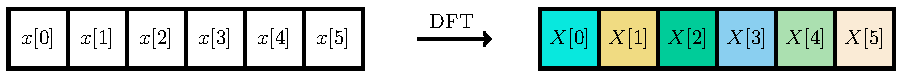
\includegraphics[width=3.1in]{X_DFT}
			\end{figure}
		\end{block}
		
		\begin{columns}
			
			\column{.47\textwidth}
			\begin{block}{{\small $\color{red}x_s$:\ Sub-sampled by $f_1=P_1=2$}}
				\begin{figure}[t]
					\centering
					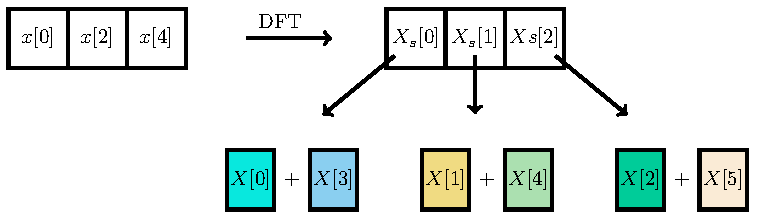
\includegraphics[width=2.3in]{Xs}
				\end{figure}
			\end{block}
			
			\begin{block}{{\small$\color{red}z_s$:\ Sub-sampled by $f_2=P_2=3$}}
				\begin{figure}[t]
					\centering
					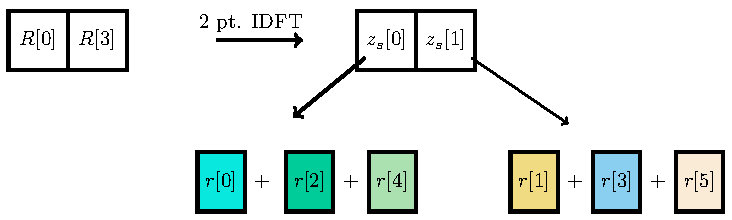
\includegraphics[width=2.3in]{Zs}
				\end{figure}
			\end{block}
			
			\column{.47\textwidth}
			\begin{block}{\small Factor graph}
				\begin{figure}[t]
					\centering
					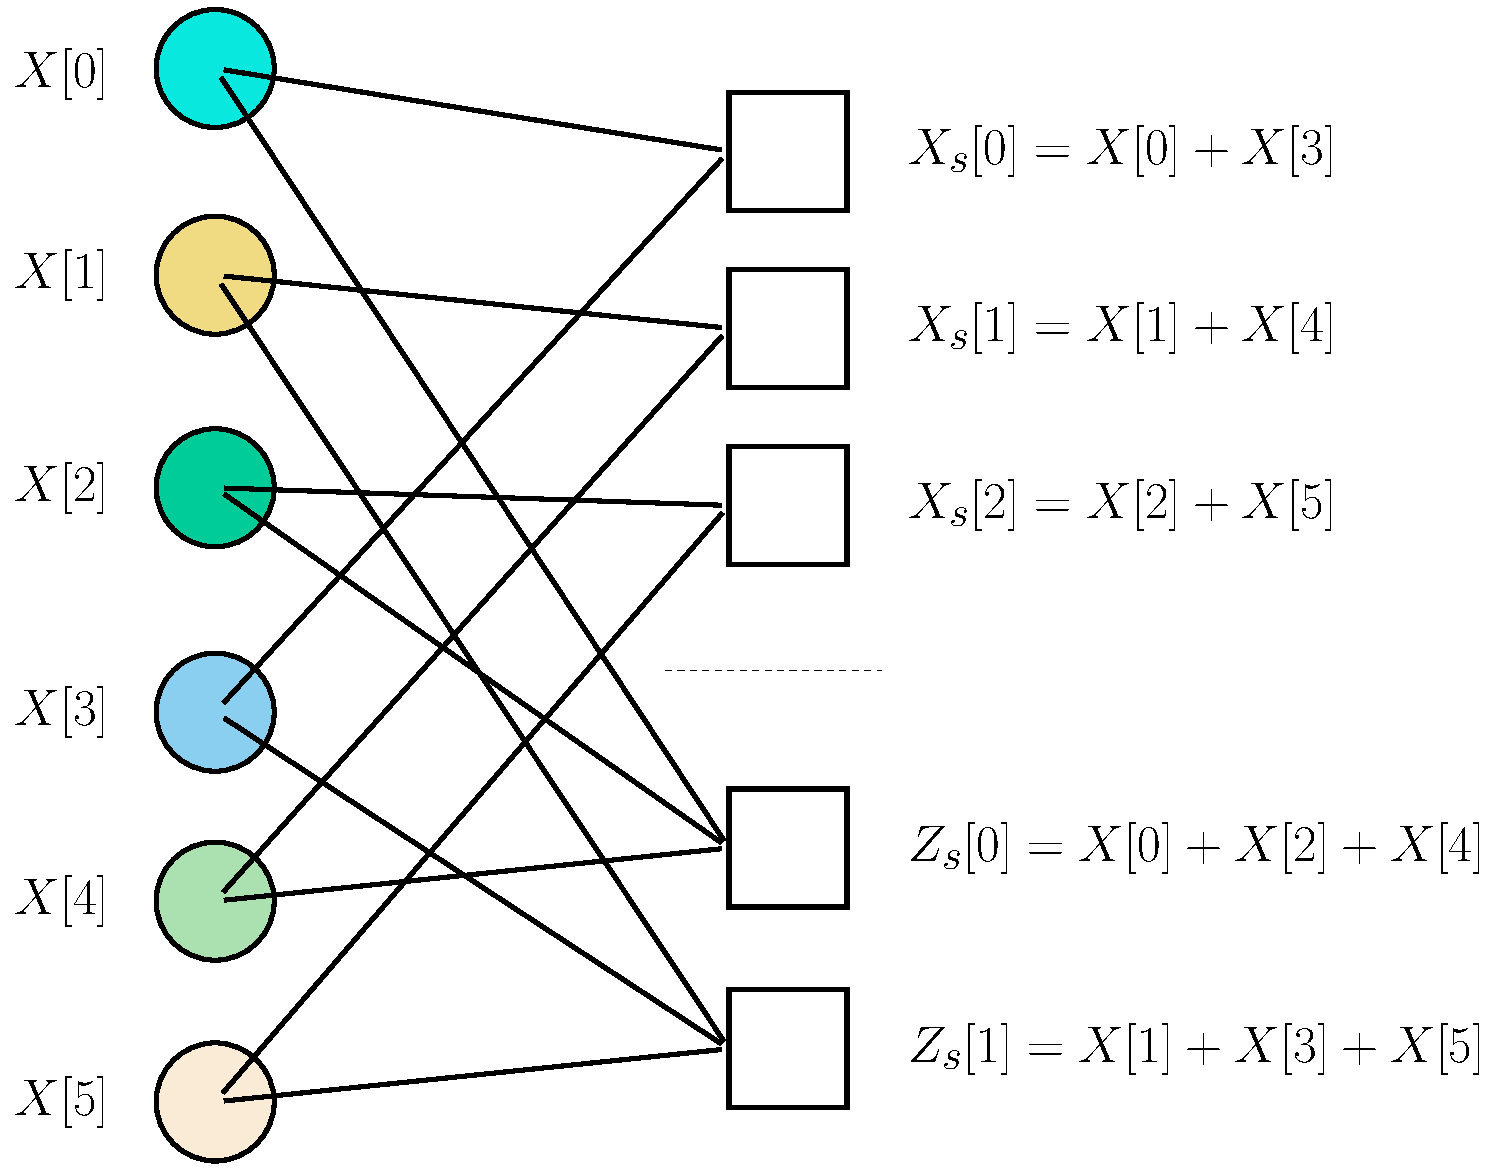
\includegraphics[width=2.3in]{Factorgraph_example}
				\end{figure}
			\end{block}
		\end{columns}
	\end{frame}
	
	
	
	%--------------------------------------------------------------------------------------
	\begin{frame}{FFAST Algorithm Example}
	%Slide-1:
	%\begin{itemize}
	%	\item Block Diagram of a simple 2-stage FFAST setup.
	%	\item Tanner Graph of the induced code with the parity equations displayed.
	%\end{itemize}
	
	\begin{figure}[t]
		\centering
		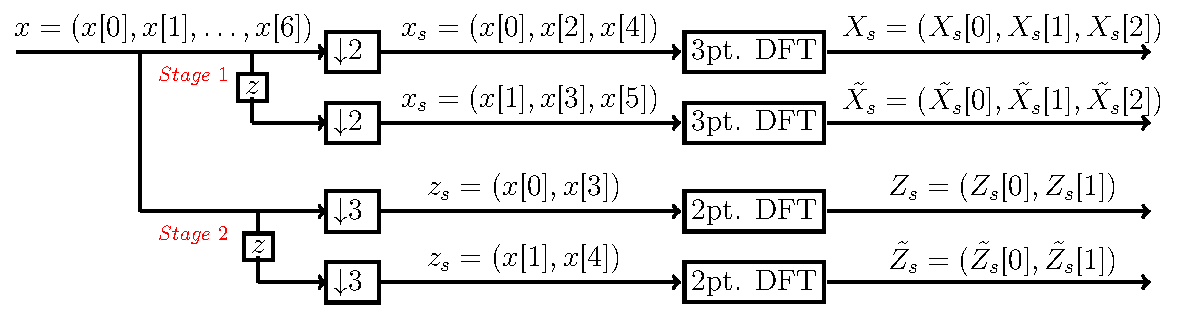
\includegraphics[width=3.6in]{FFAST_2stages_example6}
	\end{figure}
	\vspace*{-4mm}
	\begin{figure}[t]
		\includegraphics[width=2.9in]{Factorgraph_example_tilde}
	\end{figure}
	
	\end{frame}
	%------------------------------------------------------------------------------------
	\begin{frame}{Singleton Detection}
			
		%Slide-2: Singleton Detection
		%\begin{itemize}
		%	\item Tanner Graph of the induced code with the equations displayed
		%	\item Simple example explaining singleton detection (ratio test)
		%	\item Summarize the singleton detection condition. {\bf(put in slide-3 if needed)}
		%\end{itemize}
		
			\vspace{-5pt}
			\begin{figure}[t]
				
				\includegraphics[width=3.0in]{Factorgraph_example_tilde}
			\end{figure}
			\begin{block}{Singleton condition for a checknode}
			\begin{itemize}
				\item Let $i=\frac{-N}{j2\pi} \log(\frac{\tilde{X}_s[l]}{X_s[l]})$. If {\color{blue} $0 \leq i \leq N-1$}, then checknode $l$ is a \alert{Singleton}.\\
				\item $Pos(l) = i$ is the only variable node participating and $X_s[l]$ is its value.
			\end{itemize}
				
			\end{block}
			
	\end{frame}	
	%-------------------------------------------------------------------------------------
	\begin{frame}{FFAST Decoder}
		
		%Slide-3: Decoder
		%\begin{itemize}
		%	\item Tanner Graph of the induced code with the equations displayed
		%	\item Explain in few lines how the peeling decoder works for this setup
		%	\item Include a complete example with graphics that explains the complete FFAST decoder {\bf(if needed)}
		%\end{itemize}
		
%	\begin{columns}
%			\column{0.50\textwidth}
%			\begin{figure}[t]
%				\centering
%				\includegraphics[width=2.5in]{C:/Users/nrkri/Dropbox/Work/RESEARCH/Presentations/NASIT2016/Figures/FFAST_2stages}
%			\end{figure}
%			\vspace{-6mm}
%			\hspace{-1.5in}
%			\column{0.50\textwidth}
%			
%			\begin{figure}[t]
%				
%				\includegraphics[width=2.45in]{C:/Users/nrkri/Dropbox/Work/RESEARCH/Presentations/NASIT2016/Figures/Factorgraph_example_tilde}
%			\end{figure}
%			
%		\end{columns}
			\vspace{-5pt}
			\begin{figure}[t]				
%\includegraphics[width=3.0in]{C:/Users/nrkri/Dropbox/Work/RESEARCH/Presentations/NASIT2016/Figures/Factorgraph_example_tilde}
\resizebox{3.0in}{!}
{

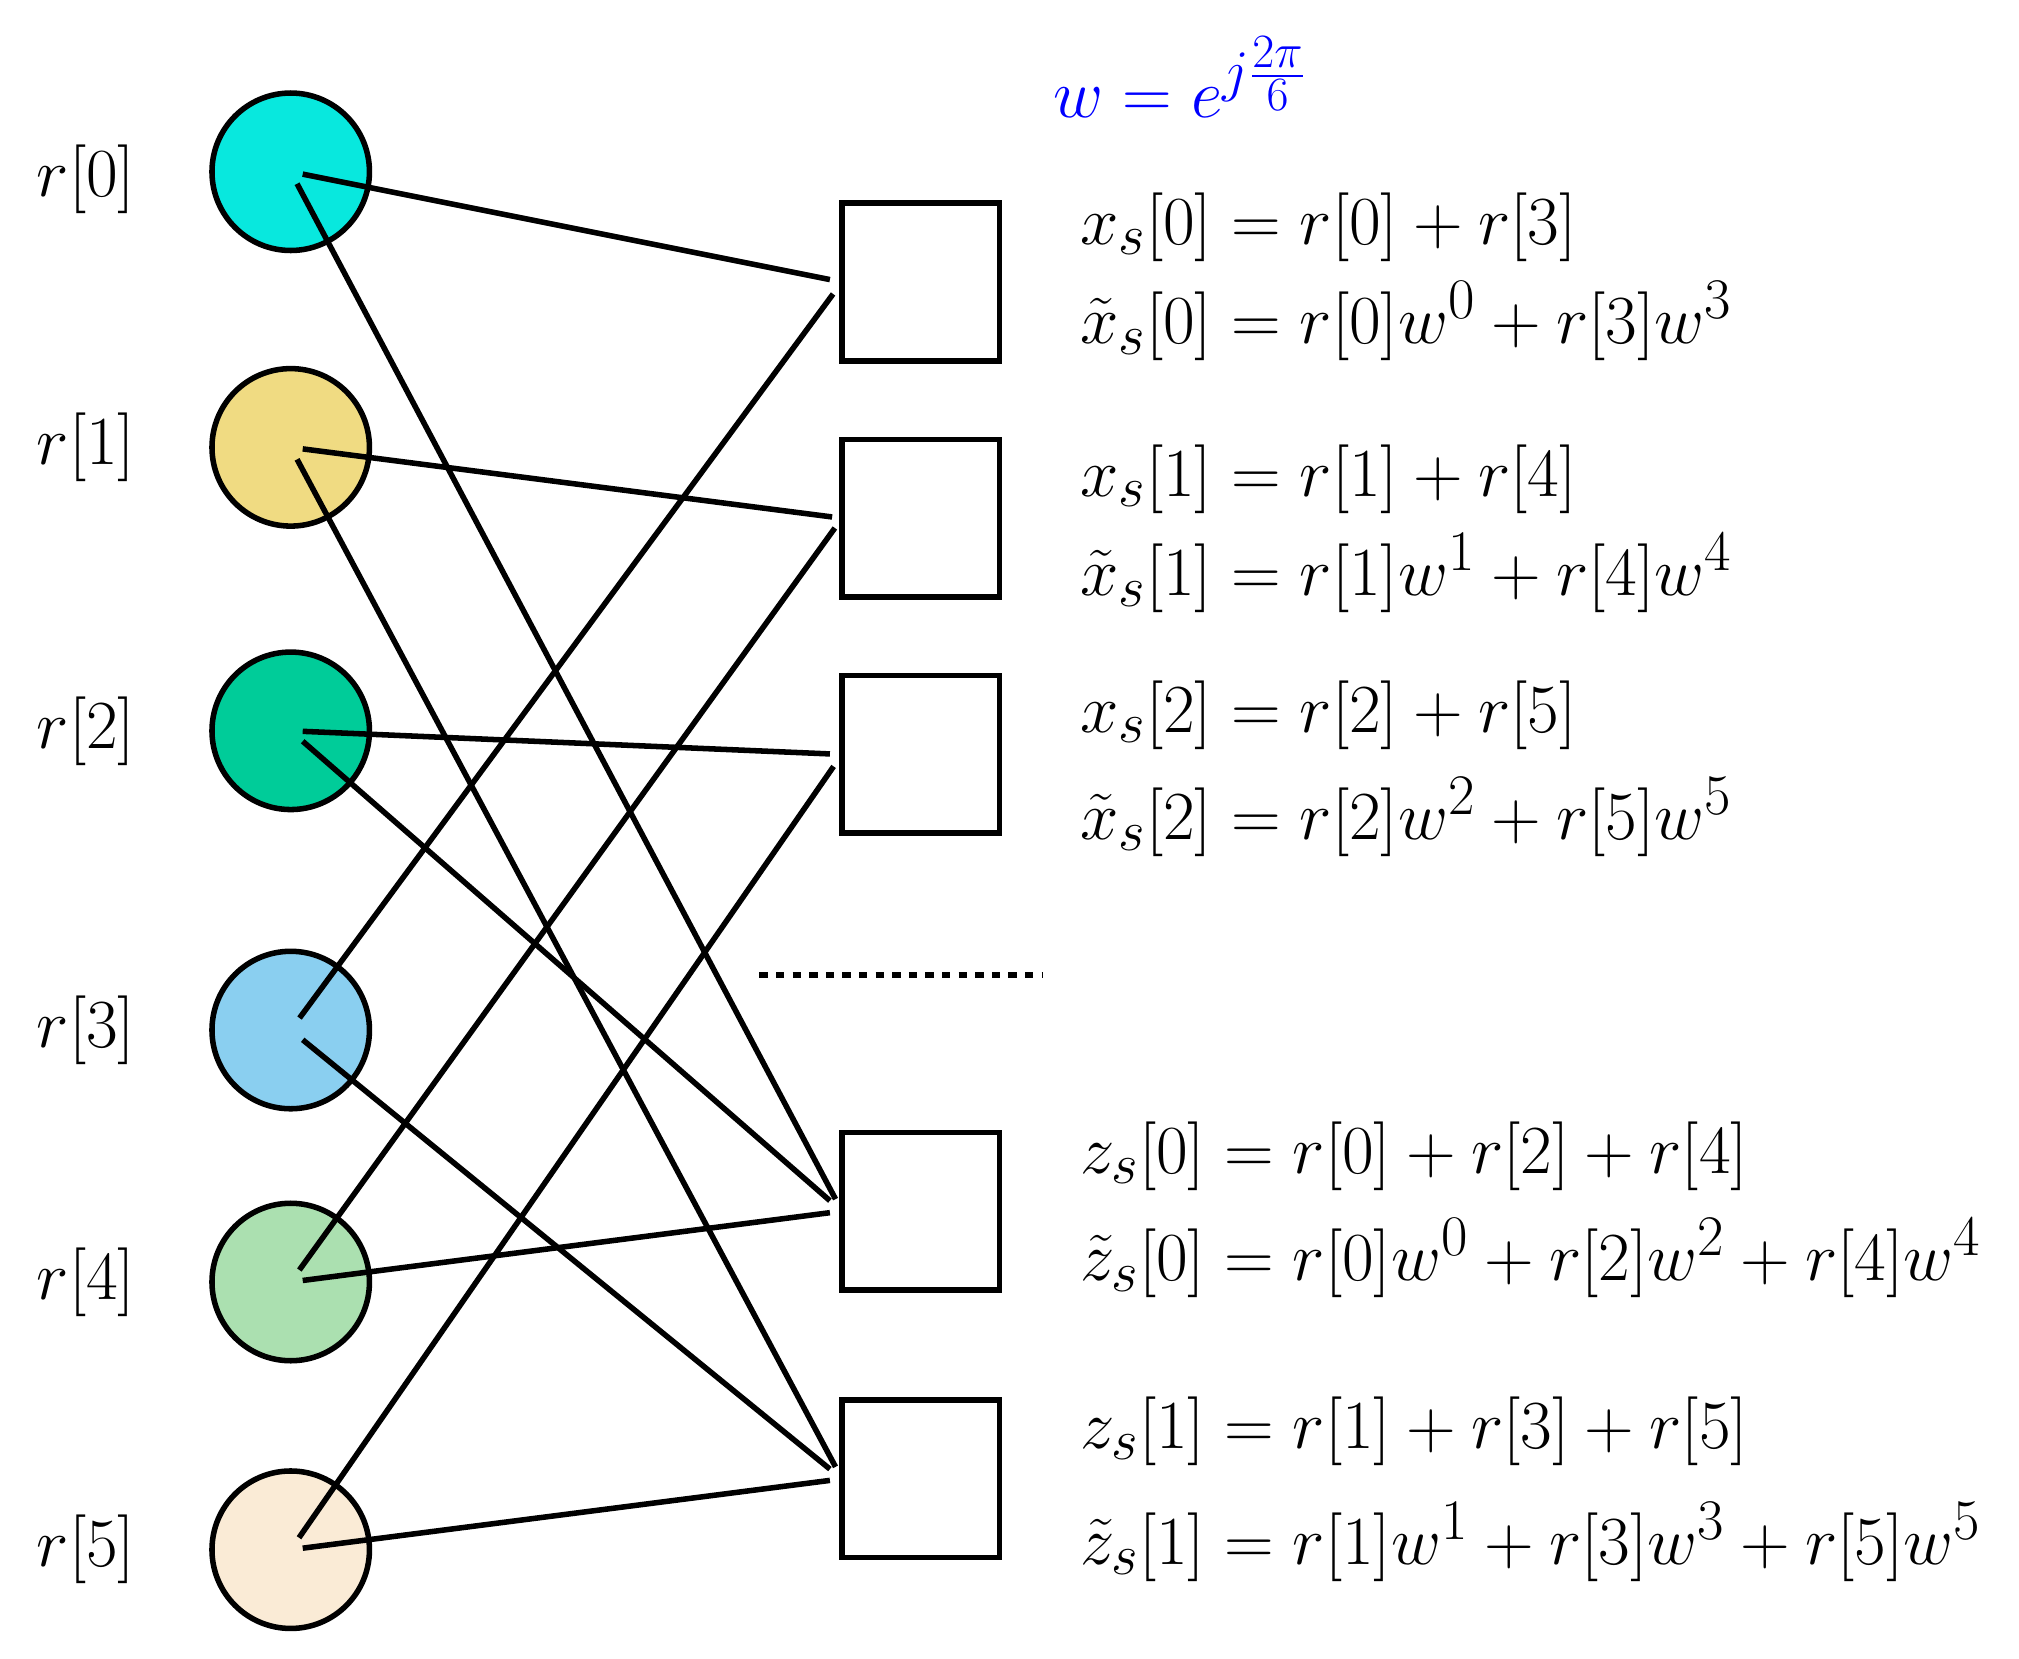
\begin{tikzpicture}

\definecolor{brightturquoise}{rgb}{0.03, 0.91, 0.87}
\definecolor{buff}{rgb}{0.94, 0.86, 0.51}
\definecolor{caribbeangreen}{rgb}{0.0, 0.8, 0.6}
\definecolor{celadon}{rgb}{0.67, 0.88, 0.69}
\definecolor{darktangerine}{rgb}{1.0, 0.66, 0.07}
\definecolor{darkviolet}{rgb}{0.58, 0.0, 0.83}
\definecolor{deepskyblue}{rgb}{0.0, 0.75, 1.0}
\definecolor{amber(sae/ece)}{rgb}{1.0, 0.49, 0.0}
\definecolor{antiquewhite}{rgb}{0.98, 0.92, 0.84}
\definecolor{applegreen}{rgb}{0.55, 0.71, 0.0}
\definecolor{babyblue}{rgb}{0.54, 0.81, 0.94}

% Variable nodes
\draw [thick,fill=babyblue,line  width =2pt]   (-7,-6) node (v6) {} ellipse (1 and 1);
\draw[thick,fill=caribbeangreen,line  width =2pt]  (-7,-2.2) node (v5) {} ellipse (1 and 1);
\draw [thick,fill=buff,line  width =2pt]  (-7,1.4) node (v3) {} ellipse (1 and 1);
\draw  [thick,fill=celadon,line  width =2pt]  (-7,-9.2) node (v1) {} ellipse (1 and 1);
\draw  [thick,fill=antiquewhite,line  width =2pt]  (-7,-12.6) node (v1_1) {} ellipse (1 and 1);
\draw  [thick,fill=brightturquoise,line  width =2pt]  (-7,4.9) node (v1_2) {} ellipse (1 and 1);
%Check nodes


\draw [thick,line  width =2pt] (0,4.5) rectangle (2,2.5);
\draw [thick,line  width =2pt]  (0,1.5) node (v8) {} rectangle (2,-0.5);
\draw [thick,line  width =2pt] (0,-1.5) rectangle (2,-3.5);




\draw [thick,line  width =2pt] (0,-7.3) rectangle (2,-9.3);
\draw [thick,line  width =2pt] (0,-10.7) rectangle (2,-12.7);



\node at (-9.6,4.8) {\Huge $r[0]$};
\node at (-9.6,1.4) {\Huge $r[1]$};
\node at (-9.6,-2.2) {\Huge $r[2]$};
\node at (-9.6,-6) {\Huge $r[3]$};
\node at (-9.6,-9.2) {\Huge $r[4]$};
\node at (-9.6,-12.6) {\Huge $r[5]$};


\node [thick,line  width =2pt] (v2) at (0,3.5) {};
\node [thick,line  width =2pt] (v4) at (0,-2.5) {};


\node [thick,line  width =2pt] (v7) at (0,-8.3) {};
\node [thick,line  width =2pt] (v9) at (0,-11.7) {};

\node [thick,line  width =2pt] (v10) at (-1.2,-5.3) {};
\node [thick,line  width =2pt] (v11) at (2.7,-5.3) {};
\draw [thick,line  width =2pt][dashed] (v10) edge (v11);
\node [anchor=west] at (2.9,4.2) {\Huge $x_{s}[0] = r[0]+r[3]$};
\node [anchor=west] at (2.9,3) {\Huge $\tilde{x}_{s}[0] = r[0] w^{0}+r[3] w^{3}$};
\node [anchor=west] at (2.9,1) {\Huge $x_{s}[1] = r[1]+r[4]$};
\node [anchor=west] at (2.9,-0.2) {\Huge $\tilde{x}_{s}[1] = r[1] w^{1}+r[4] w^{4}$};
\node [anchor=west] at (2.9,-2) {\Huge $x_{s}[2] = r[2]+r[5]$};
\node [anchor=west] at (2.9,-3.3) {\Huge $\tilde{x}_{s}[2] = r[2] w^{2}+r[5] w^{5}$};

\node [anchor=west] at (2.9,-7.6) {\Huge $z_{s}[0] = r[0]+r[2]+r[4]$};
\node [anchor=west] at (2.9,-8.9) {\Huge $\tilde{z}_{s}[0] = r[0] w^{0}+r[2] w^{2}+r[4] w^{4}$};
\node [anchor=west] at (2.9,-11.1) {\Huge $z_{s}[1] = r[1]+r[3]+r[5]$};
\node [anchor=west] at (2.9,-12.5) {\Huge $\tilde{z}_{s}[1] = r[1] w^{1}+r[3] w^{3}+r[5] w^{5}$};

\draw [thick,line  width =2pt] (v1_2) edge (v2);
\draw [thick,line  width =2pt] (v1_2) edge (v7);

\draw [thick,line  width =2pt] (v3) edge (v9);
\draw [thick,line  width =2pt] (v5) edge (v4);
\node (v12) at (0,0.5) {};
\draw [thick,line  width =2pt] (v3) edge (v12);
\draw [thick,line  width =2pt] (v5) edge (v7);

\draw [thick,line  width =2pt] (v6) edge (v2);
\draw [thick,line  width =2pt](v1) edge (v12);
\draw [thick,line  width =2pt] (v1_1) edge (v4);
\draw [thick,line  width =2pt] (v6) edge (v9);
\draw [thick,line  width =2pt] (v1_1) edge (v9);
\draw [thick,line  width =2pt] (v1) edge (v7);
\node at (4.3,6.1) {\color{blue} \Huge$w=e^{j \frac{2\pi}{6} }$};
\end{tikzpicture}

}
			\end{figure}

		\begin{block}{Peeling decoder}
			\begin{itemize}
				\item 1 non-zero value among the neighbors of any right node can be recovered
								
				\item Iteratively errors can be corrected and analyzed for random non-zero coeffs
			\end{itemize}
		\end{block}
	\end{frame}	
	%-----------------------------------------------------------------------------------------
	\begin{frame}{FFAST Decoder Example}
	\only<1-3>{\begin{block}{Example 1}
		Let $N=6$, and the non-zero coefficients be X[0]=5, X[3]=4, X[4]=7
	    \end{block}	}
	    \vspace{-7pt}
		\begin{columns}
			\only<2-3>{
				\column{0.43\textwidth}
                \resizebox{2.0in}{!}
                {
                
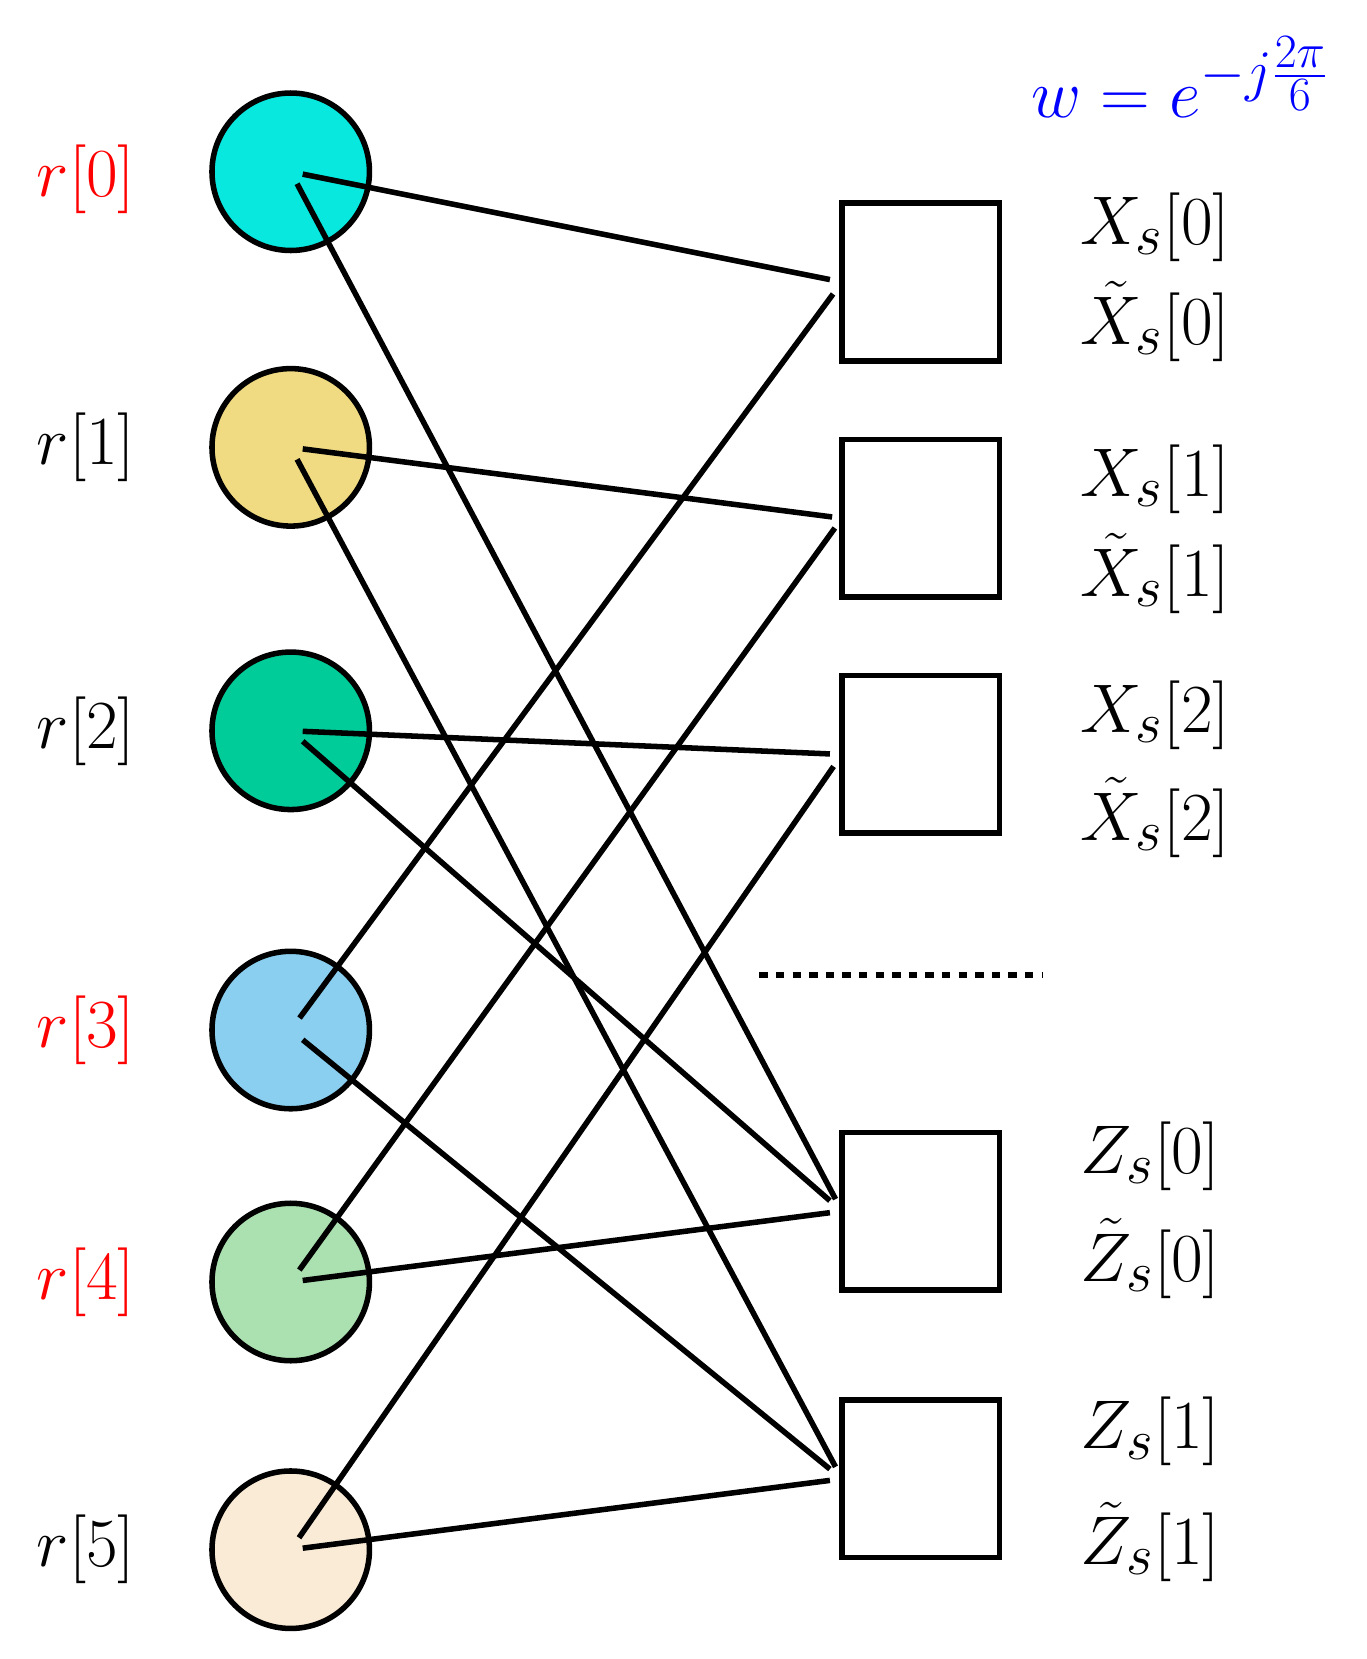
\begin{tikzpicture}

\definecolor{brightturquoise}{rgb}{0.03, 0.91, 0.87}
\definecolor{buff}{rgb}{0.94, 0.86, 0.51}
\definecolor{caribbeangreen}{rgb}{0.0, 0.8, 0.6}
\definecolor{celadon}{rgb}{0.67, 0.88, 0.69}
\definecolor{darktangerine}{rgb}{1.0, 0.66, 0.07}
\definecolor{darkviolet}{rgb}{0.58, 0.0, 0.83}
\definecolor{deepskyblue}{rgb}{0.0, 0.75, 1.0}
\definecolor{amber(sae/ece)}{rgb}{1.0, 0.49, 0.0}
\definecolor{antiquewhite}{rgb}{0.98, 0.92, 0.84}
\definecolor{applegreen}{rgb}{0.55, 0.71, 0.0}
\definecolor{babyblue}{rgb}{0.54, 0.81, 0.94}

% Variable nodes
\draw [thick,fill=babyblue,line  width =2pt]   (-7,-6) node (v6) {} ellipse (1 and 1);
\draw[thick,fill=caribbeangreen,line  width =2pt]  (-7,-2.2) node (v5) {} ellipse (1 and 1);
\draw [thick,fill=buff,line  width =2pt]  (-7,1.4) node (v3) {} ellipse (1 and 1);
\draw  [thick,fill=celadon,line  width =2pt]  (-7,-9.2) node (v1) {} ellipse (1 and 1);
\draw  [thick,fill=antiquewhite,line  width =2pt]  (-7,-12.6) node (v1_1) {} ellipse (1 and 1);
\draw  [thick,fill=brightturquoise,line  width =2pt]  (-7,4.9) node (v1_2) {} ellipse (1 and 1);
%Check nodes


\draw [thick,line  width =2pt] (0,4.5) rectangle (2,2.5);
\draw [thick,line  width =2pt]  (0,1.5) node (v8) {} rectangle (2,-0.5);
\draw [thick,line  width =2pt] (0,-1.5) rectangle (2,-3.5);




\draw [thick,line  width =2pt] (0,-7.3) rectangle (2,-9.3);
\draw [thick,line  width =2pt] (0,-10.7) rectangle (2,-12.7);



\node at (-9.6,4.8) {\color{red}{\Huge $r[0]$}};
\node at (-9.6,1.4) {\Huge $r[1]$};
\node at (-9.6,-2.2) {\Huge $r[2]$};
\node at (-9.6,-6) {\color{red}{\Huge $r[3]$}};
\node at (-9.6,-9.2) {\color{red}{\Huge $r[4]$}};
\node at (-9.6,-12.6) {\Huge $r[5]$};


\node [thick,line  width =2pt] (v2) at (0,3.5) {};
\node [thick,line  width =2pt] (v4) at (0,-2.5) {};


\node [thick,line  width =2pt] (v7) at (0,-8.3) {};
\node [thick,line  width =2pt] (v9) at (0,-11.7) {};

\node [thick,line  width =2pt] (v10) at (-1.2,-5.3) {};
\node [thick,line  width =2pt] (v11) at (2.7,-5.3) {};
\draw [thick,line  width =2pt][dashed] (v10) edge (v11);
\node [anchor=west] at (2.9,4.2) {\Huge $X_{s}[0]$};
\node [anchor=west] at (2.9,3) {\Huge $\tilde{X}_{s}[0]$};
\node [anchor=west] at (2.9,1) {\Huge $X_{s}[1]$};
\node [anchor=west] at (2.9,-0.2) {\Huge $\tilde{X}_{s}[1]$};
\node [anchor=west] at (2.9,-2) {\Huge $X_{s}[2]$};
\node [anchor=west] at (2.9,-3.3) {\Huge $\tilde{X}_{s}[2]$};

\node [anchor=west] at (2.9,-7.6) {\Huge $Z_{s}[0]$};
\node [anchor=west] at (2.9,-8.9) {\Huge $\tilde{Z}_{s}[0]$};
\node [anchor=west] at (2.9,-11.1) {\Huge $Z_{s}[1]$};
\node [anchor=west] at (2.9,-12.5) {\Huge $\tilde{Z}_{s}[1]$};

\draw [thick,line  width =2pt] (v1_2) edge (v2);
\draw [thick,line  width =2pt] (v1_2) edge (v7);

\draw [thick,line  width =2pt] (v3) edge (v9);
\draw [thick,line  width =2pt] (v5) edge (v4);
\node (v12) at (0,0.5) {};
\draw [thick,line  width =2pt] (v3) edge (v12);
\draw [thick,line  width =2pt] (v5) edge (v7);

\draw [thick,line  width =2pt] (v6) edge (v2);
\draw [thick,line  width =2pt](v1) edge (v12);
\draw [thick,line  width =2pt] (v1_1) edge (v4);
\draw [thick,line  width =2pt] (v6) edge (v9);
\draw [thick,line  width =2pt] (v1_1) edge (v9);
\draw [thick,line  width =2pt] (v1) edge (v7);
\node at (4.3,6.1) {\color{blue} \Huge$w=e^{-j \frac{2\pi}{6} }$};
\end{tikzpicture}

                }

				\column{0.55\textwidth}
        \vspace{-7pt}
				\begin{figure}[t]	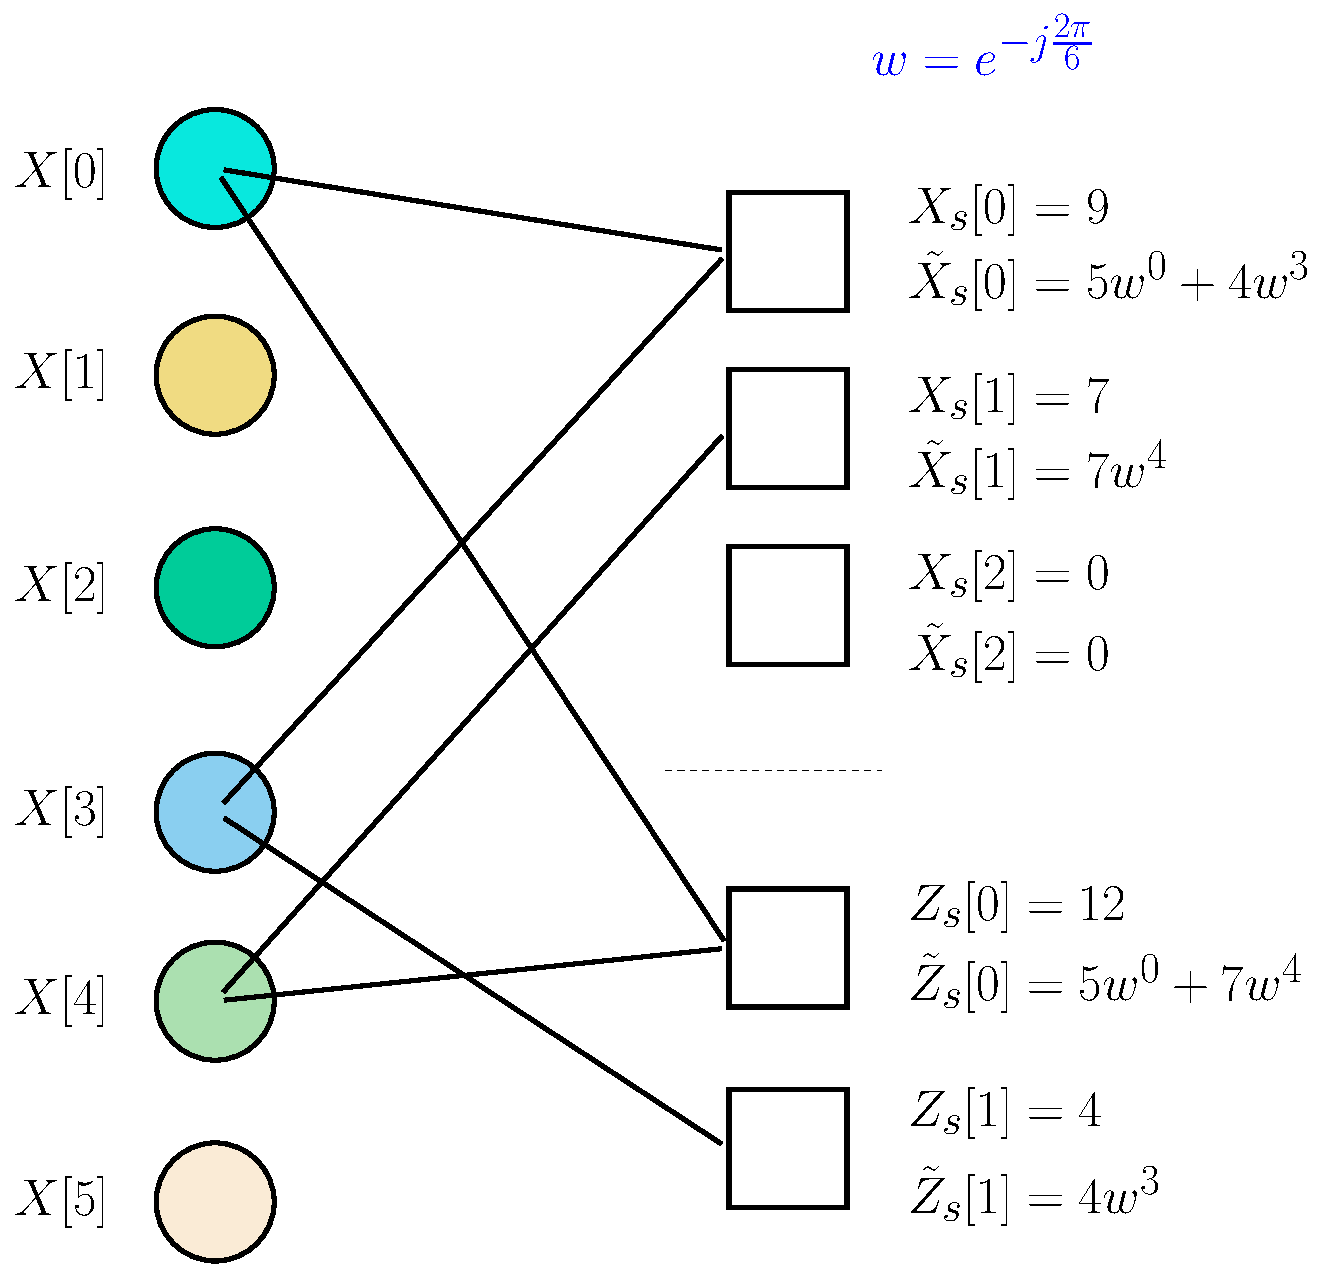
\includegraphics[width=2.6in]{Factorgraph_example1_tilde}
				\end{figure}}
				%\column{0.25\textwidth}
				%\only<3>{\large \color{green} Yes, recoverable!}			
		\end{columns}
		
		\vspace{-7pt}
		
%	\only<4-6>{
%		
%		 \begin{block}{Example 2}
%		Let $N=6$, and the non-zero coefficients be X[0] = 5,X[1] = 3 , X[2]=1, X[3] = 4, X[4] = 7.
%	     \end{block}}
%	     \begin{columns}	
%	
%	     \column{0.70\textwidth}
%	\only<5->{\begin{figure}[t]		
%			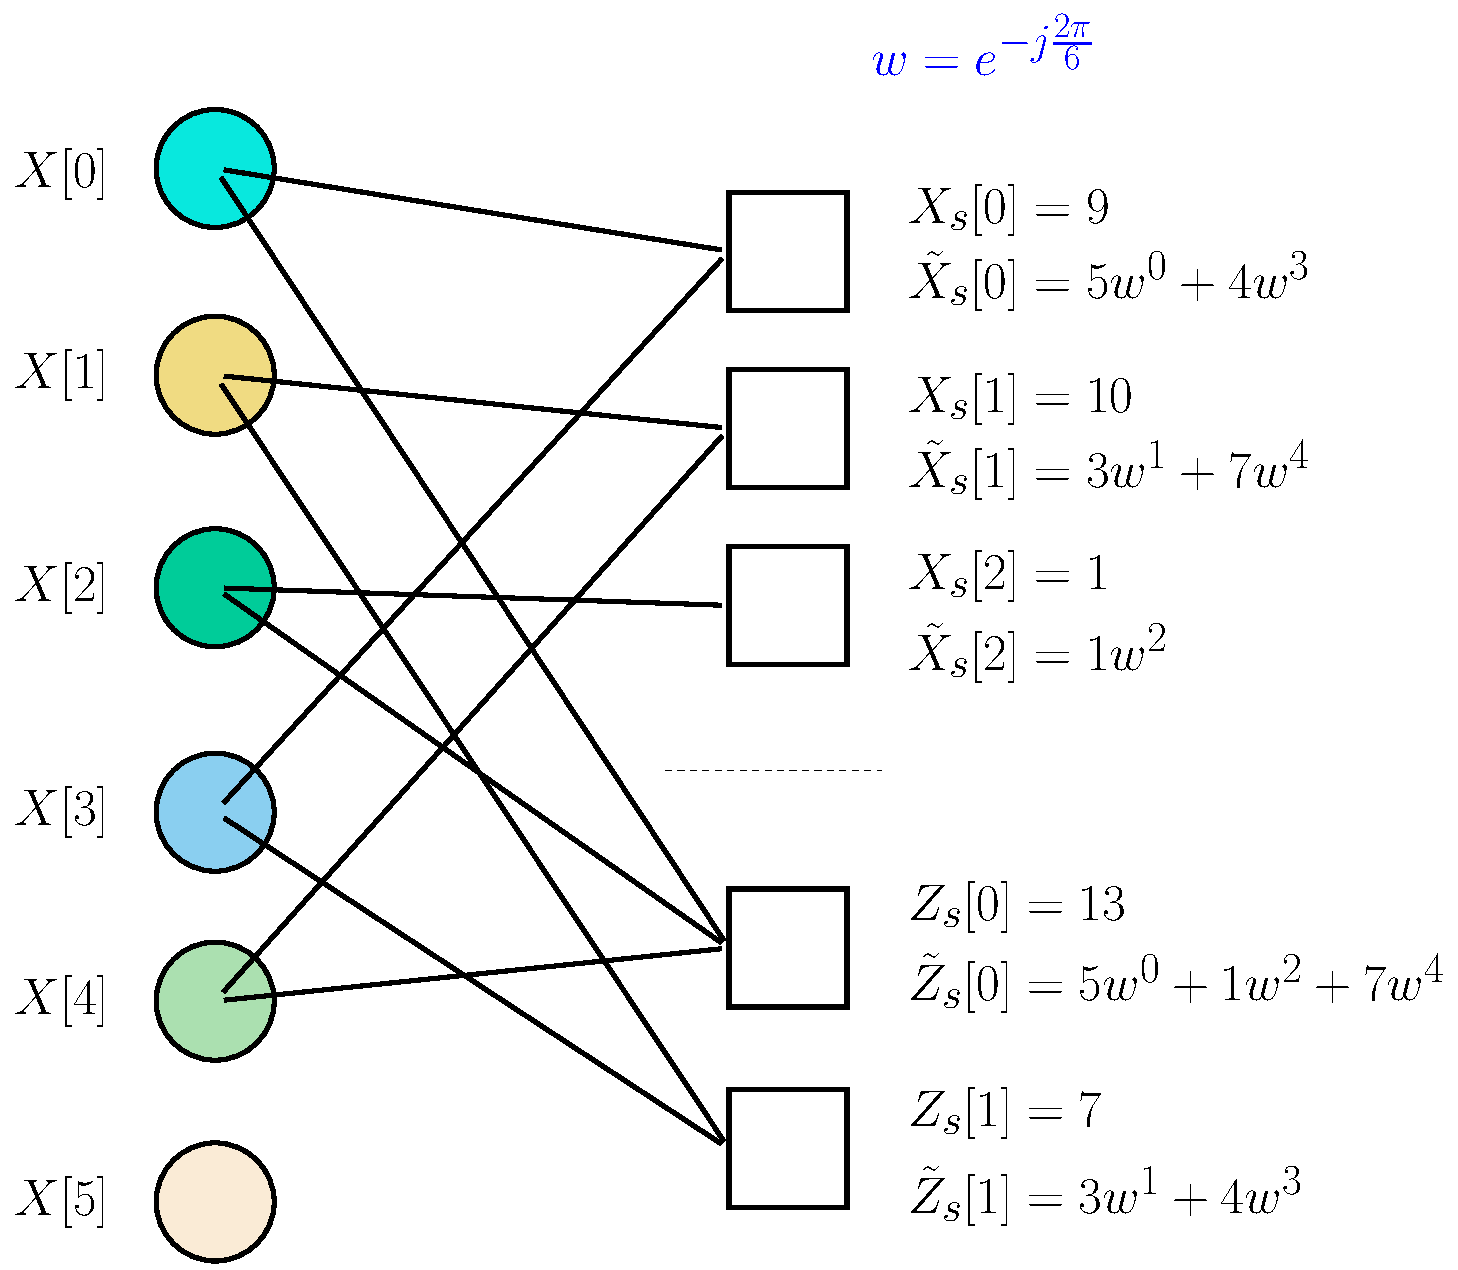
\includegraphics[width=2.6in]{C:/Users/nrkri/Dropbox/Work/RESEARCH/Presentations/NASIT2016/Figures/Factorgraph_example2_tilde}
%		      \end{figure}}
%	   	\column{0.30\textwidth}
%		\only<6>{\Large \alert{ Not recoverable!}}
%	\end{columns}		
	\end{frame}
%	
	%-----------------------------------------------------------------------------------------
%	\begin{frame}{FFAST Construction For Different Regimes}
%%	\begin{itemize}
%%		\item Figure: Block diagram of the a d-staged FFAST setup with generalized down-sampling parameter
%%		\item Give the values of the down-sampling parameters for less-sparse and very-sparse regime. (Also, give the aliasing equations for each case {\bf(if needed)}).
%%		\item Include the generalized FFAST construction for each $\delta$ ranges {\bf(if needed)}
%%	\end{itemize}	
%
%	\begin{figure}[t]
%		\includegraphics[width=3.0in]{C:/Users/nrkri/Dropbox/Work/RESEARCH/Presentations/NASIT2016/Figures/FFAST_2stages}
%	\end{figure}
%	
%	
%
%			Let, $N=P_1 \times P_2 \times \ldots P_d$
%	\begin{columns}
%		\column{0.4\textwidth}
%		
%		
%		\begin{block}{\alert{Very-sparse regime}}
%			\begin{itemize}
%				\item $K = O(N^\delta), 0<\delta \leq 1/3$
%				\item \textcolor{blue}{$f_i= N/P_i,\ i=1,2, \ldots,d$}
%				\end{itemize}
%				\end{block}
%				
%				\column{0.4\textwidth}
%				\begin{block}{\alert{Less-sparse regime}}
%					\begin{itemize}
%						\item $K = O(N^\delta), 1/3<\delta \leq 1$
%						\item \textcolor{blue}{$f_i= P_i,\ i=1,2, \ldots,d$}
%						\end{itemize}
%						\end{block}
%						
%						\end{columns}
%							
%
%			\end{frame}
	%-------------------------------------------------------------------------------------
	\begin{frame}{Generalization}
		
		%Slide-3: Decoder
		%\begin{itemize}
		%	\item Tanner Graph of the induced code with the equations displayed
		%	\item Explain in few lines how the peeling decoder works for this setup
		%	\item Include a complete example with graphics that explains the complete FFAST decoder {\bf(if needed)}
		%\end{itemize}
		
	\begin{columns}
			\column{0.50\textwidth}
			\begin{figure}[t]
				\centering
				\includegraphics[width=2.5in]{FFAST_2stages}
			\end{figure}
			\vspace{-6mm}
			\hspace{-1.5in}
			\column{0.50\textwidth}
			
			\begin{figure}[t]
				
				\includegraphics[width=2.45in]{Factorgraph_example_tilde}
			\end{figure}
			
		\end{columns}
%			\vspace{-5pt}
%			\begin{figure}[t]
%				
%				\includegraphics[width=2.75in]{C:/Users/nrkri/Dropbox/Work/RESEARCH/Presentations/NASIT2016/Figures/Factorgraph_example_tilde}
%			\end{figure}
		\begin{block}{Reed Solomon component codes}
			\begin{itemize}
				\item $(X_s[l_1],\tilde{X}_s[l_1])$ correspond to 2 syndromes of a 1-error correcting RS code
                \item RS is over the complex field, no miscorrection
			\end{itemize}
		\end{block}
	\end{frame}	



%---------------------------------------------------------
\begin{frame}\frametitle{Sparse Fourier Transform Approach}
	\begin{figure}[t]
		\centering
		\scalebox{0.28}{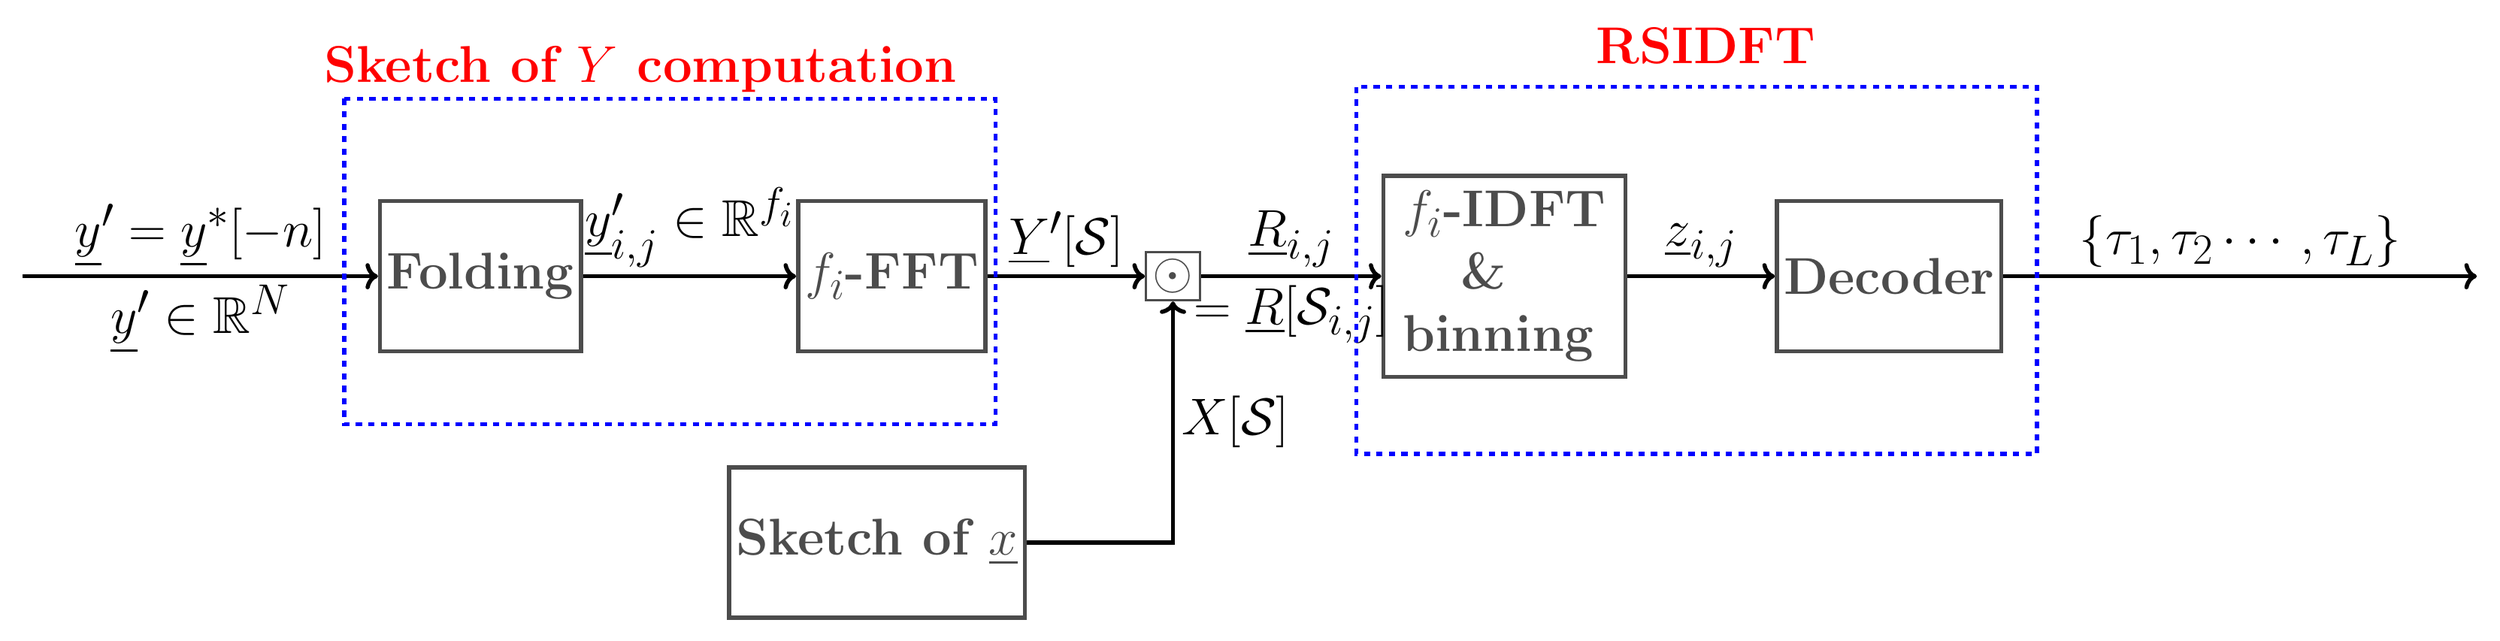
\begin{tikzpicture}

\def\nodewidth{1in}
\def\fsize{\Huge}
\tikzstyle{block} = [rectangle, draw, thick,opacity=0.7,line width =2, minimum size=\nodewidth]
\tikzstyle{opnode} = [rectangle, draw, thick,opacity=0.7,line width=1, minimum size=0.2in]

\node[block] (r1) at (-8.7,3){\fsize \bf Folding};
\node[block] (r2) at (-1.75,3) {\fsize \bf $f_i$-FFT};
\node[opnode] (r3) at (3,3) {\fsize \bf $\odot$};
\node[block,align=center] (r4) at (8.6,3) {\fsize \bf \begin{tabular}{l}
$f_i$-IDFT \\ 
~~ \& \\ 
binning
\end{tabular}};
\node[block] (r5) at (15.1,3) {\fsize \bf Decoder};
\node[block] (r6) at (-2,-1.5) {\fsize \bf Sketch of $\xv$};


\draw[<-, thick, line width=2] (r1.west)--node[midway, above]{\fsize $\yv'=\yv^*[-n]$}
node[midway, below]{\fsize $\yv'\in\mathbb{R}^N$}+(-6,0);
\draw[->, thick, line width=2] (r1.east)--node[midway, above]{\fsize $\yv'_{i,j}\in\mathbb{R}^{f_i}$}(r2.west);
\draw[->, thick, line width=2] (r2.east)--node[midway, above]{\fsize $\Yv'[\mc{S}]$}(r3.west);
\draw[->, thick, line width=2] (r3.east)--node[midway, above]{\fsize $\Rv_{i,j}$}
node[midway,below]{\fsize \bf $=\Rv[\mathcal{S}_{i,j}]$}(r4.west);
\draw[->, thick, line width=2] (r4.east)--node[midway, above]{\fsize $\zv_{i,j}$}(r5.west);
\draw[->, thick, line width=2] (r5.east)--node[midway, above]{\fsize $\{\tau_1, \tau_2 \cdots, \tau_L \}$}+(8,0);
\draw[->, thick, line width=2] let \p1=(r6),\p2= (r3) in (r6.east)--(\x2,\y1)--node[midway, right]{\fsize \bf $X[\mathcal{S}]$}  (r3.south);



\draw [dashed, line width =2, color=blue] (-11,6) rectangle (0,0.5);
\node[color= red] at (-6,6.5) {\fsize \bf  Sketch of $Y$ computation};
\draw [dashed, line width =2, color=blue]  (6.1,6.2) rectangle (17.6,0);
\node [color = red] at (12,6.9) {\fsize \bf RSIDFT};
\end{tikzpicture}}
	\end{figure}
\begin{itemize}
\item In the pattern matching problem we want to recover a sparse IDFT
\item FFT $\Leftrightarrow$ IFFT duality can be used
\end{itemize}
\end{frame}
%--------------------------------------------------------------------------------------------------------
\begin{frame}\frametitle{RSIDFT Framework}
	\begin{itemize}
    \item $N = f_1 \ f_2 \ldots \ f_d$ where $f_i \approx N^\alpha$
    \item Subsample by $N^{1-\alpha} \Rightarrow$ aliasing from $N^{1-\alpha}$ coeffs
    \end{itemize}
		\begin{figure}[t!]
			\begin{center}
				\resizebox{0.7\textwidth}{!}{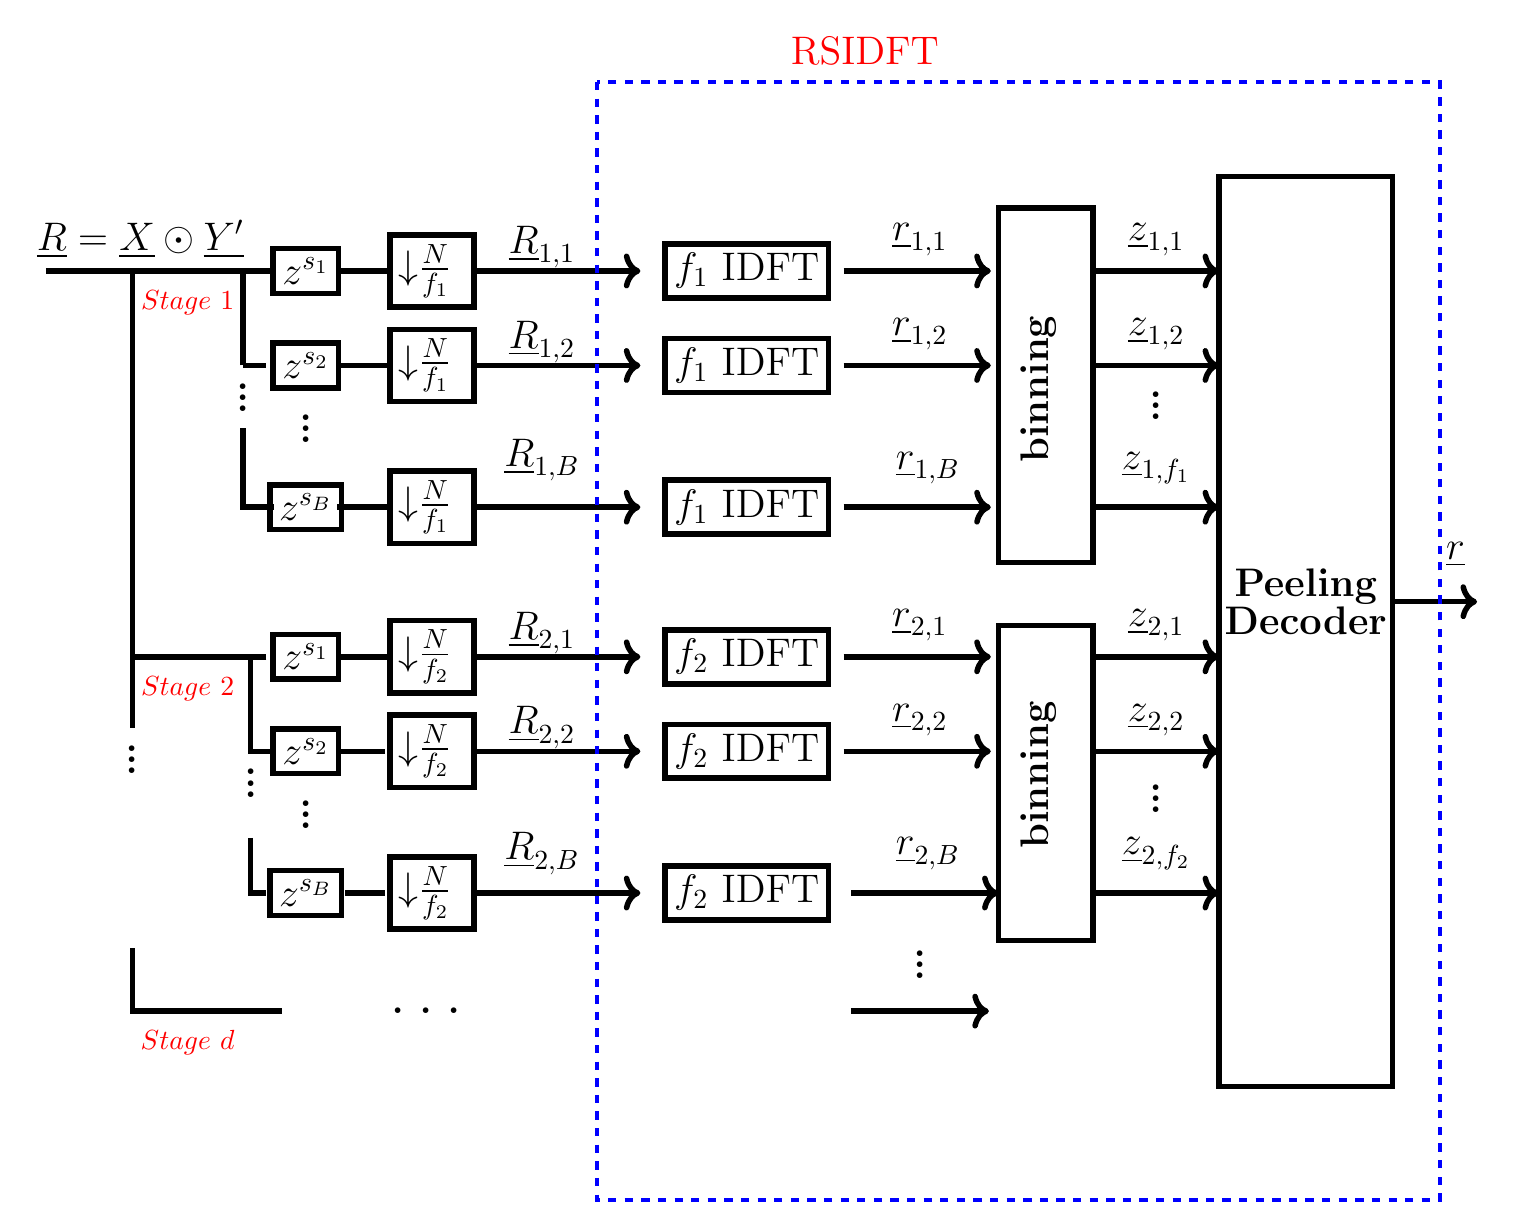
\begin{tikzpicture}

 % Downsampling blocks
\node[draw,align=center,thick,line  width =2pt] at (1.8,4.5) {\Large{$\mathbf{\downarrow} \frac{N}{f_2}$} };
\node[draw,align=center,thick,line  width =2pt] at (1.8,5.7) {\Large{$\mathbf{\downarrow} \frac{N}{f_2}$ }};
\node[draw,align=center,thick,line  width =2pt] (v6) at (1.8,2.7) {\Large{$\mathbf{\downarrow} \frac{N}{f_2}$ }};

\node[draw,align=center,thick,line  width =2pt] at (1.8,9.4) {\Large{$\mathbf{\downarrow} \frac{N}{f_1}$} };
\node[draw,align=center,thick,line  width =2pt] at (1.8,10.6) {\Large{$\mathbf{\downarrow} \frac{N}{f_1}$ }};
\node[draw,align=center,thick,line  width =2pt] at (1.8,7.6) {\Large{$\mathbf{\downarrow} \frac{N}{f_1}$ }};

%  Input lines to the down-sampling block

%  Delay blocks
\node[draw,align=center,thick,line  width =2pt] at (0.2,10.6) {\bf \Large{$z^{s_1}$}};
\node[draw,align=center,thick,line  width =2pt] at (0.2,9.4) {\bf \Large{$z^{s_2}$}};
\node[draw,align=center,thick,line  width =2pt] at (0.2,7.6) {\bf \Large{$z^{s_B}$}};

\node[draw,align=center,thick,line  width =2pt] at (0.2,5.7) {\bf \Large{$z^{s_1}$}};
\node[draw,align=center,thick,line  width =2pt] at (0.2,4.5) {\bf \Large{$z^{s_2}$}};
\node[draw,align=center,thick,line  width =2pt] at (0.2,2.7) {\bf \Large{$z^{s_B}$}};


% paths connecting the delay blocks  
 
 \draw[thick,line  width =2pt] (1.3,9.4) -- (0.6,9.4);
 

\node[line  width =2pt] at (-0.6,9.1) {\Huge{\vdots}};
\node[line  width =2pt] at (0.2,8.7) {\Huge{\vdots}};
\node[line  width =2pt] at (-0.5,4.2) {\Huge{\vdots}};
\node[line  width =2pt] at (0.2,3.8) {\Huge{\vdots}};

 \draw[thick,line  width =2pt] (1.3,10.6) -- (0.6,10.6);
 \draw[thick,line  width =2pt] (-0.6,9.4) -- (-0.6,10.6);
 
% paths connecting the two stages   
 \draw[thick,line  width =2pt] (-0.2,10.6) -- (-2,10.6);
 \draw[thick,line  width =2pt] (-0.6,9.4) -- (-0.3,9.4);
 \draw[thick,line  width =2pt] (-0.3,5.7) -- (-2,5.7);
 \draw[thick,line  width =2pt] (-2,5.7) -- (-2,10.6);
  \draw[thick,line  width =2pt] (-3.1,10.6) -- (-2,10.6);
  \draw[thick,line  width =2pt] (-2,5.7) -- (-2,4.8);
  
  
  % DFT blocks
\node[draw,align=center,thick,line  width =2pt] at (5.8,4.5) {\Large{$f_2$ IDFT}};
\node[draw,align=center,thick,line  width =2pt] at (5.8,5.7) {\Large{$f_2$ IDFT}};
\node[draw,align=center,thick,line  width =2pt] at (5.8,2.7) {\Large{$f_2$ IDFT}};

\node[draw,align=center,thick,line  width =2pt] at (5.8,9.4) {\Large{$f_1$ IDFT}};
\node[draw,align=center,thick,line  width =2pt] at (5.8,10.6) {\Large{$f_1$ IDFT}};
\node[draw,align=center,thick,line  width =2pt] at (5.8,7.6) {\Large{$f_1$ IDFT}};
% Connectors
 \draw[->,thick,line  width =2pt] (2.35,10.6) -- (4.45,10.6);
 \draw[->,thick,line  width =2pt] (2.35,9.4) -- (4.45,9.4);
 \draw[->,thick,line  width =2pt] (2.35,7.6) -- (4.45,7.6);
 
 \draw[->,thick,line  width =2pt] (2.35,5.7) -- (4.45,5.7);
 \draw[->,thick,line  width =2pt] (2.35,4.5) -- (4.45,4.5);
 \draw[->,thick,line  width =2pt] (2.35,2.7) -- (4.45,2.7);

 \draw[->,thick,line  width =2pt] (10.23,10.6) -- (11.8,10.6);
 \draw[->,thick,line  width =2pt] (10.23,9.4) -- (11.8,9.4);
 \draw[->,thick,line  width =2pt] (10.23,7.6) -- (11.8,7.6);
 
 \draw[->,thick,line  width =2pt] (10.23,5.7) -- (11.8,5.7);
 \draw[->,thick,line  width =2pt] (10.23,4.5) -- (11.8,4.5);
 \draw[->,thick,line  width =2pt] (10.23,2.7) -- (11.8,2.7);
 
  \draw[->,thick,line  width =2pt] (7.03,10.6) -- (8.9,10.6);
 \draw[->,thick,line  width =2pt] (7.03,9.4) -- (8.9,9.4);
 \draw[->,thick,line  width =2pt] (7.03,7.6) -- (8.9,7.6);
 
 \draw[->,thick,line  width =2pt] (7.03,5.7) -- (8.9,5.7);
 \draw[->,thick,line  width =2pt] (7.03,4.5) -- (8.9,4.5);
 \draw[->,thick,line  width =2pt] (7.13,2.7) -- (9,2.7);
 
  % Labels
  \node[draw=none,align=center] at (-1.9,11) {\Large{$\Rv= \underline{X} \odot \underline{Y'}$}};
  
  \node[draw=none,align=center] at (3.2,10.9) {\Large{$\Rv_{1,1}$}};
  \node[draw=none,align=center] at (3.2,9.7) {\Large{$\Rv_{1,2}$}};
\node[draw=none,align=center] at (3.2,8.2) {\Large{$\Rv_{1,B}$}};

\node[draw=none,align=center] at (3.2,6) {\Large{$\Rv_{2,1}$}};
  \node[draw=none,align=center] at (3.2,4.8) {\Large{$\Rv_{2,2}$}};
  \node[draw=none,align=center] at (3.2,3.2) {\Large{$\Rv_{2,B}$}};

  \node[draw=none,align=center] at (8,11) {\Large{$\rv_{1,1}$}};
  \node[draw=none,align=center] at (8,9.8) {\Large{$\rv_{1,2}$}};
  \node[draw=none,align=center] at (8.1,8.1) {\Large{$\rv_{1,B}$}};
  
    \node[draw=none,align=center] at (11,11) {\Large{$\zv_{1,1}$}};
  \node[draw=none,align=center] at (11,9.8) {\Large{$\zv_{1,2}$}};
  \node[draw=none,align=center] at (11,8.1) {\Large{$\zv_{1,f_1}$}};
  
     \node [draw=none] at (11,9) {\Huge{\vdots}} ;
   
  \node[draw=none,align=center] at (8,6.1) {\Large{$\rv_{2,1}$}};
  \node[draw=none,align=center] at (8,4.9) {\Large{$\rv_{2,2}$}};
  \node[draw=none,align=center] at (8.1,3.2) {\Large{$\rv_{2,B}$}};
  
  \node [draw=none] at (11,4) {\Huge{\vdots}} ;
  
    \node[draw=none,align=center] at (11,6.1) {\Large{$\zv_{2,1}$}};
  \node[draw=none,align=center] at (11,4.9) {\Large{$\zv_{2,2}$}};
  \node[draw=none,align=center] at (11,3.2) {\Large{$\zv_{2,f_2}$}};
  
  \node [draw=none] at (-2,4.5) {\Huge{\vdots}} ;
  
   \node[draw=none,align=center] at (-1.3,10.2) {\color{red}$Stage ~1$};
  \node[draw=none,align=center] at (-1.3,5.3) {\color{red}$Stage ~2$};
   \node[draw=none,align=center] at (-1.3,0.8) {\color{red}$Stage ~d$};
\draw [thick,line  width =2pt](-2,2) -- (-2,1.2) -- (-0.1,1.2) ;
 \node[draw=none,align=center] at (1.8,1.2) {\Huge{\ldots}};
 
\draw [thick,line  width =2pt] (11.8,0.2424) rectangle (14,11.8);
\node (v1) at (7,1.2) {};
\node (v2) at (9,1.2) {};



\node (v11) at (1.3,7.6) {};


\draw  [->,thick,line  width =2pt](v1) edge (v2);
\node at (8,1.9) {\Huge{\vdots}};
\node [text width=3cm, align =center ] at (12.9,6.4) {\Large \bf Peeling \\ Decoder};
\node (v3) at (13.9,6.4) {};
\node (v4) at (15.2,6.4) {};
\draw [thick, ->,line  width =2pt] (v3) edge (v4);
\node at (14.8,7) {\Large{$\rv$}};

\draw[thick,line  width =2pt] (-0.6,8.6) -- (-0.6,7.6) -- (-0.2,7.6);
\draw[thick,line  width =2pt] (0.6,7.6) -- (1.3,7.6);
\draw[thick,line  width =2pt] (-0.5,5.7) -- (-0.5,4.5) -- (-0.2,4.5);
\draw[thick,line  width =2pt] (-0.5,3.4) -- (-0.5,2.7) -- (-0.3,2.7);
\draw [thick,line  width =2pt](0.6,5.7) -- (1.3,5.7);
\draw[thick,line  width =2pt] (0.6,4.5) -- (1.2,4.5);
\draw[thick,line  width =2pt] (0.7,2.7) -- (1.2,2.7);
\draw [dashed, color=blue, line width =1.5pt ] (3.9,13) rectangle (14.6,-1.2);
\node[color =red] at (7.3,13.4) {\Large RSIDFT  };
\draw [thick, line width =2pt]  (9,11.4) rectangle (10.2,6.9);
\draw [thick, line width =2pt]  (9,6.1) rectangle (10.2,2.1);
\node[rotate=90] at (9.5,9.1) {\Large \bf binning};
\node[rotate=90] at (9.5,4.2) {\Large \bf binning};
\end{tikzpicture}}
				%	 		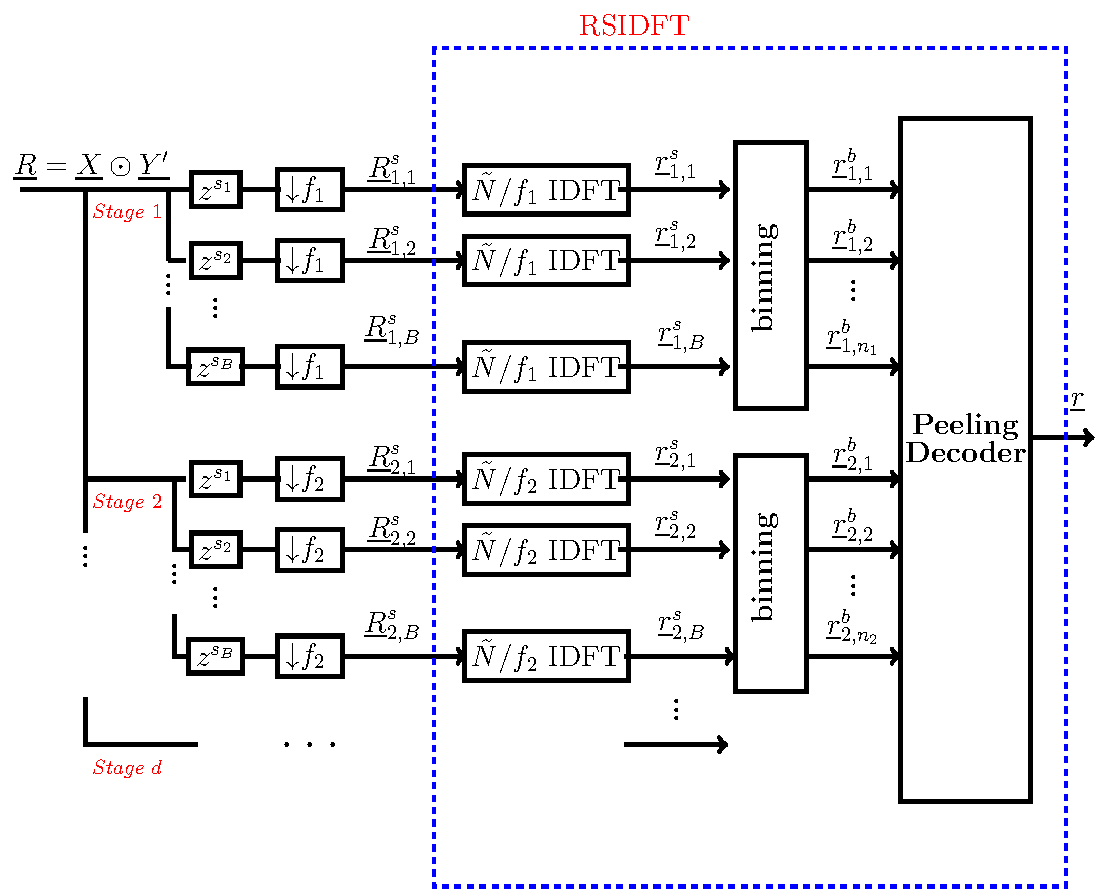
\includegraphics[height=7cm]{Figures/FFAST_Robust}
			\end{center}	
			\label{fig:rsidft}
			\vspace{5 pt}
		\end{figure}
\end{frame}
%--------------------------------------------------------------------------------------------------------
\begin{frame}\frametitle{RSIDFT-Decoding (Peeling Decoder)}
\begin{columns}
	\column[]{0.65\columnwidth}
		\begin{figure}[h!]
			\begin{center}
				%		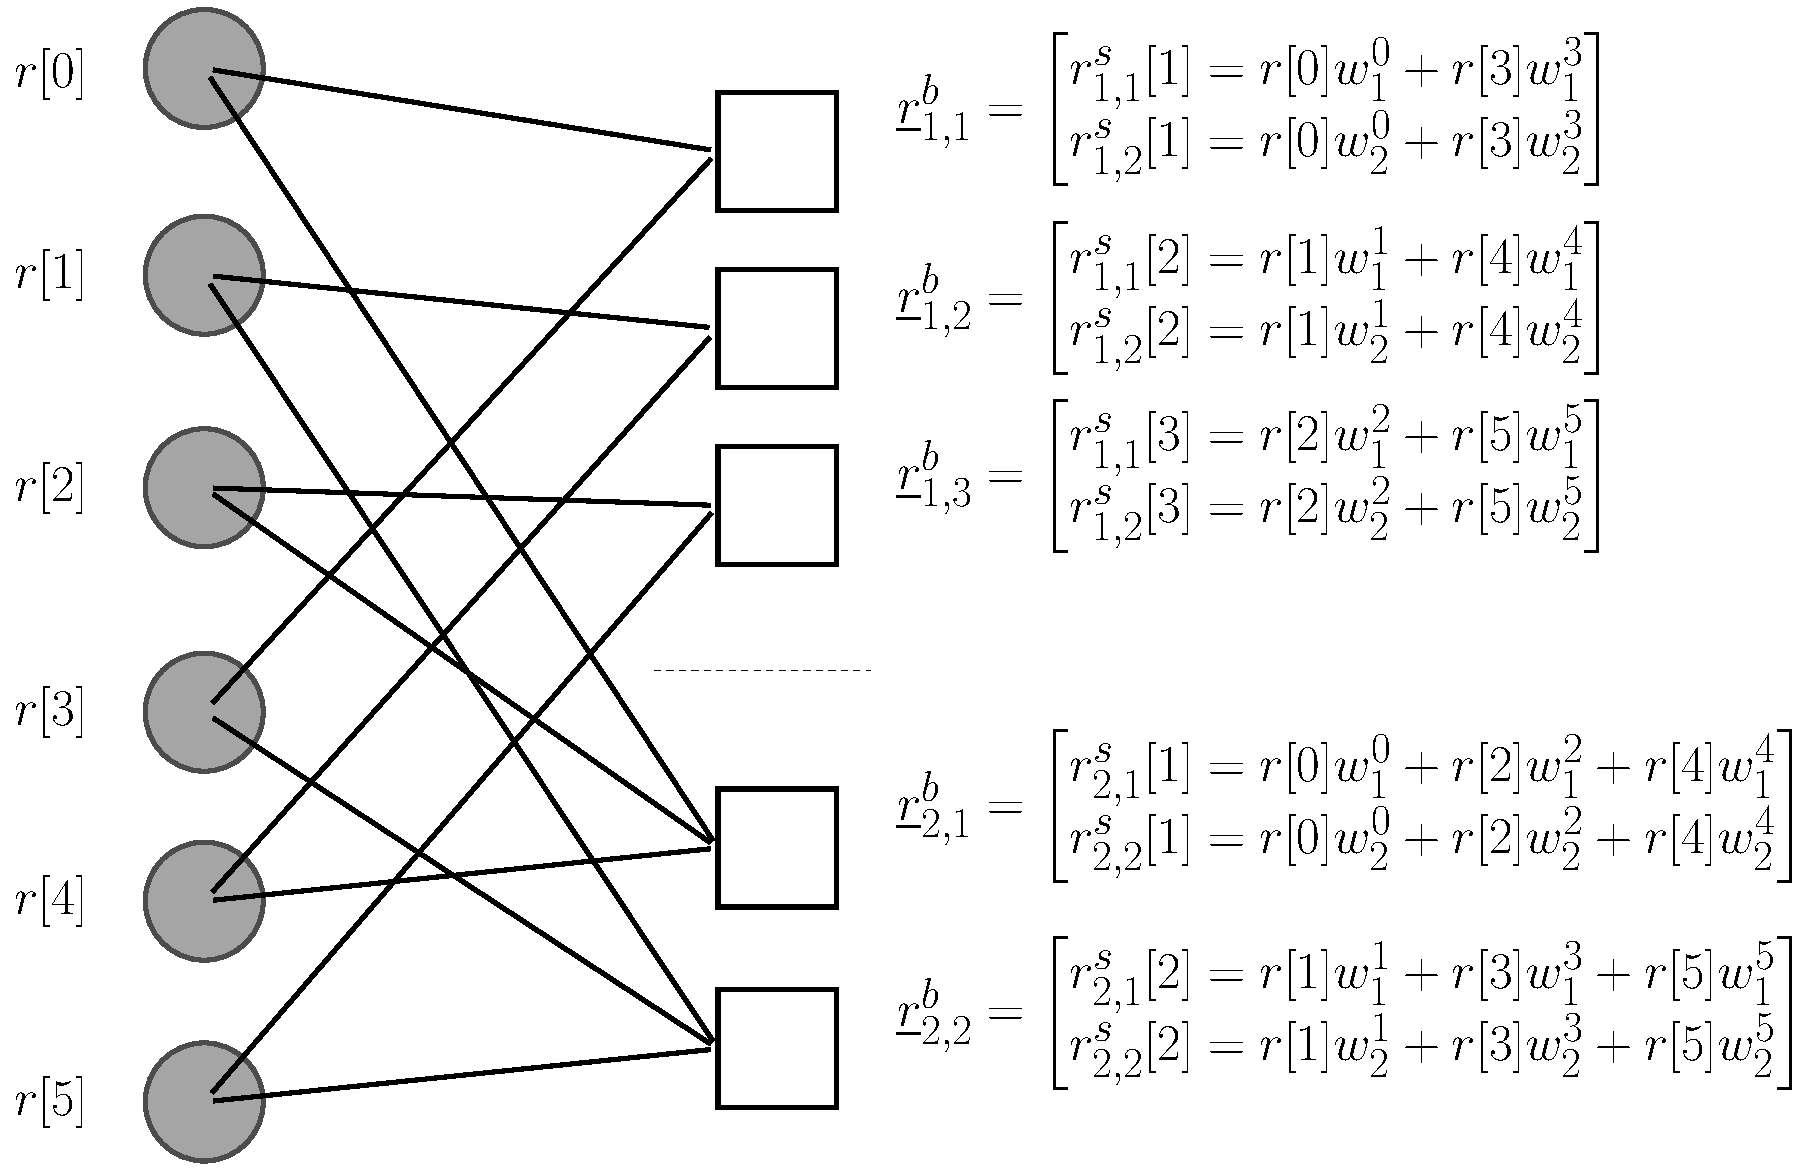
\includegraphics[height=7cm]{Figures/Factorgraph}
				\resizebox{1.0\textwidth}{!}{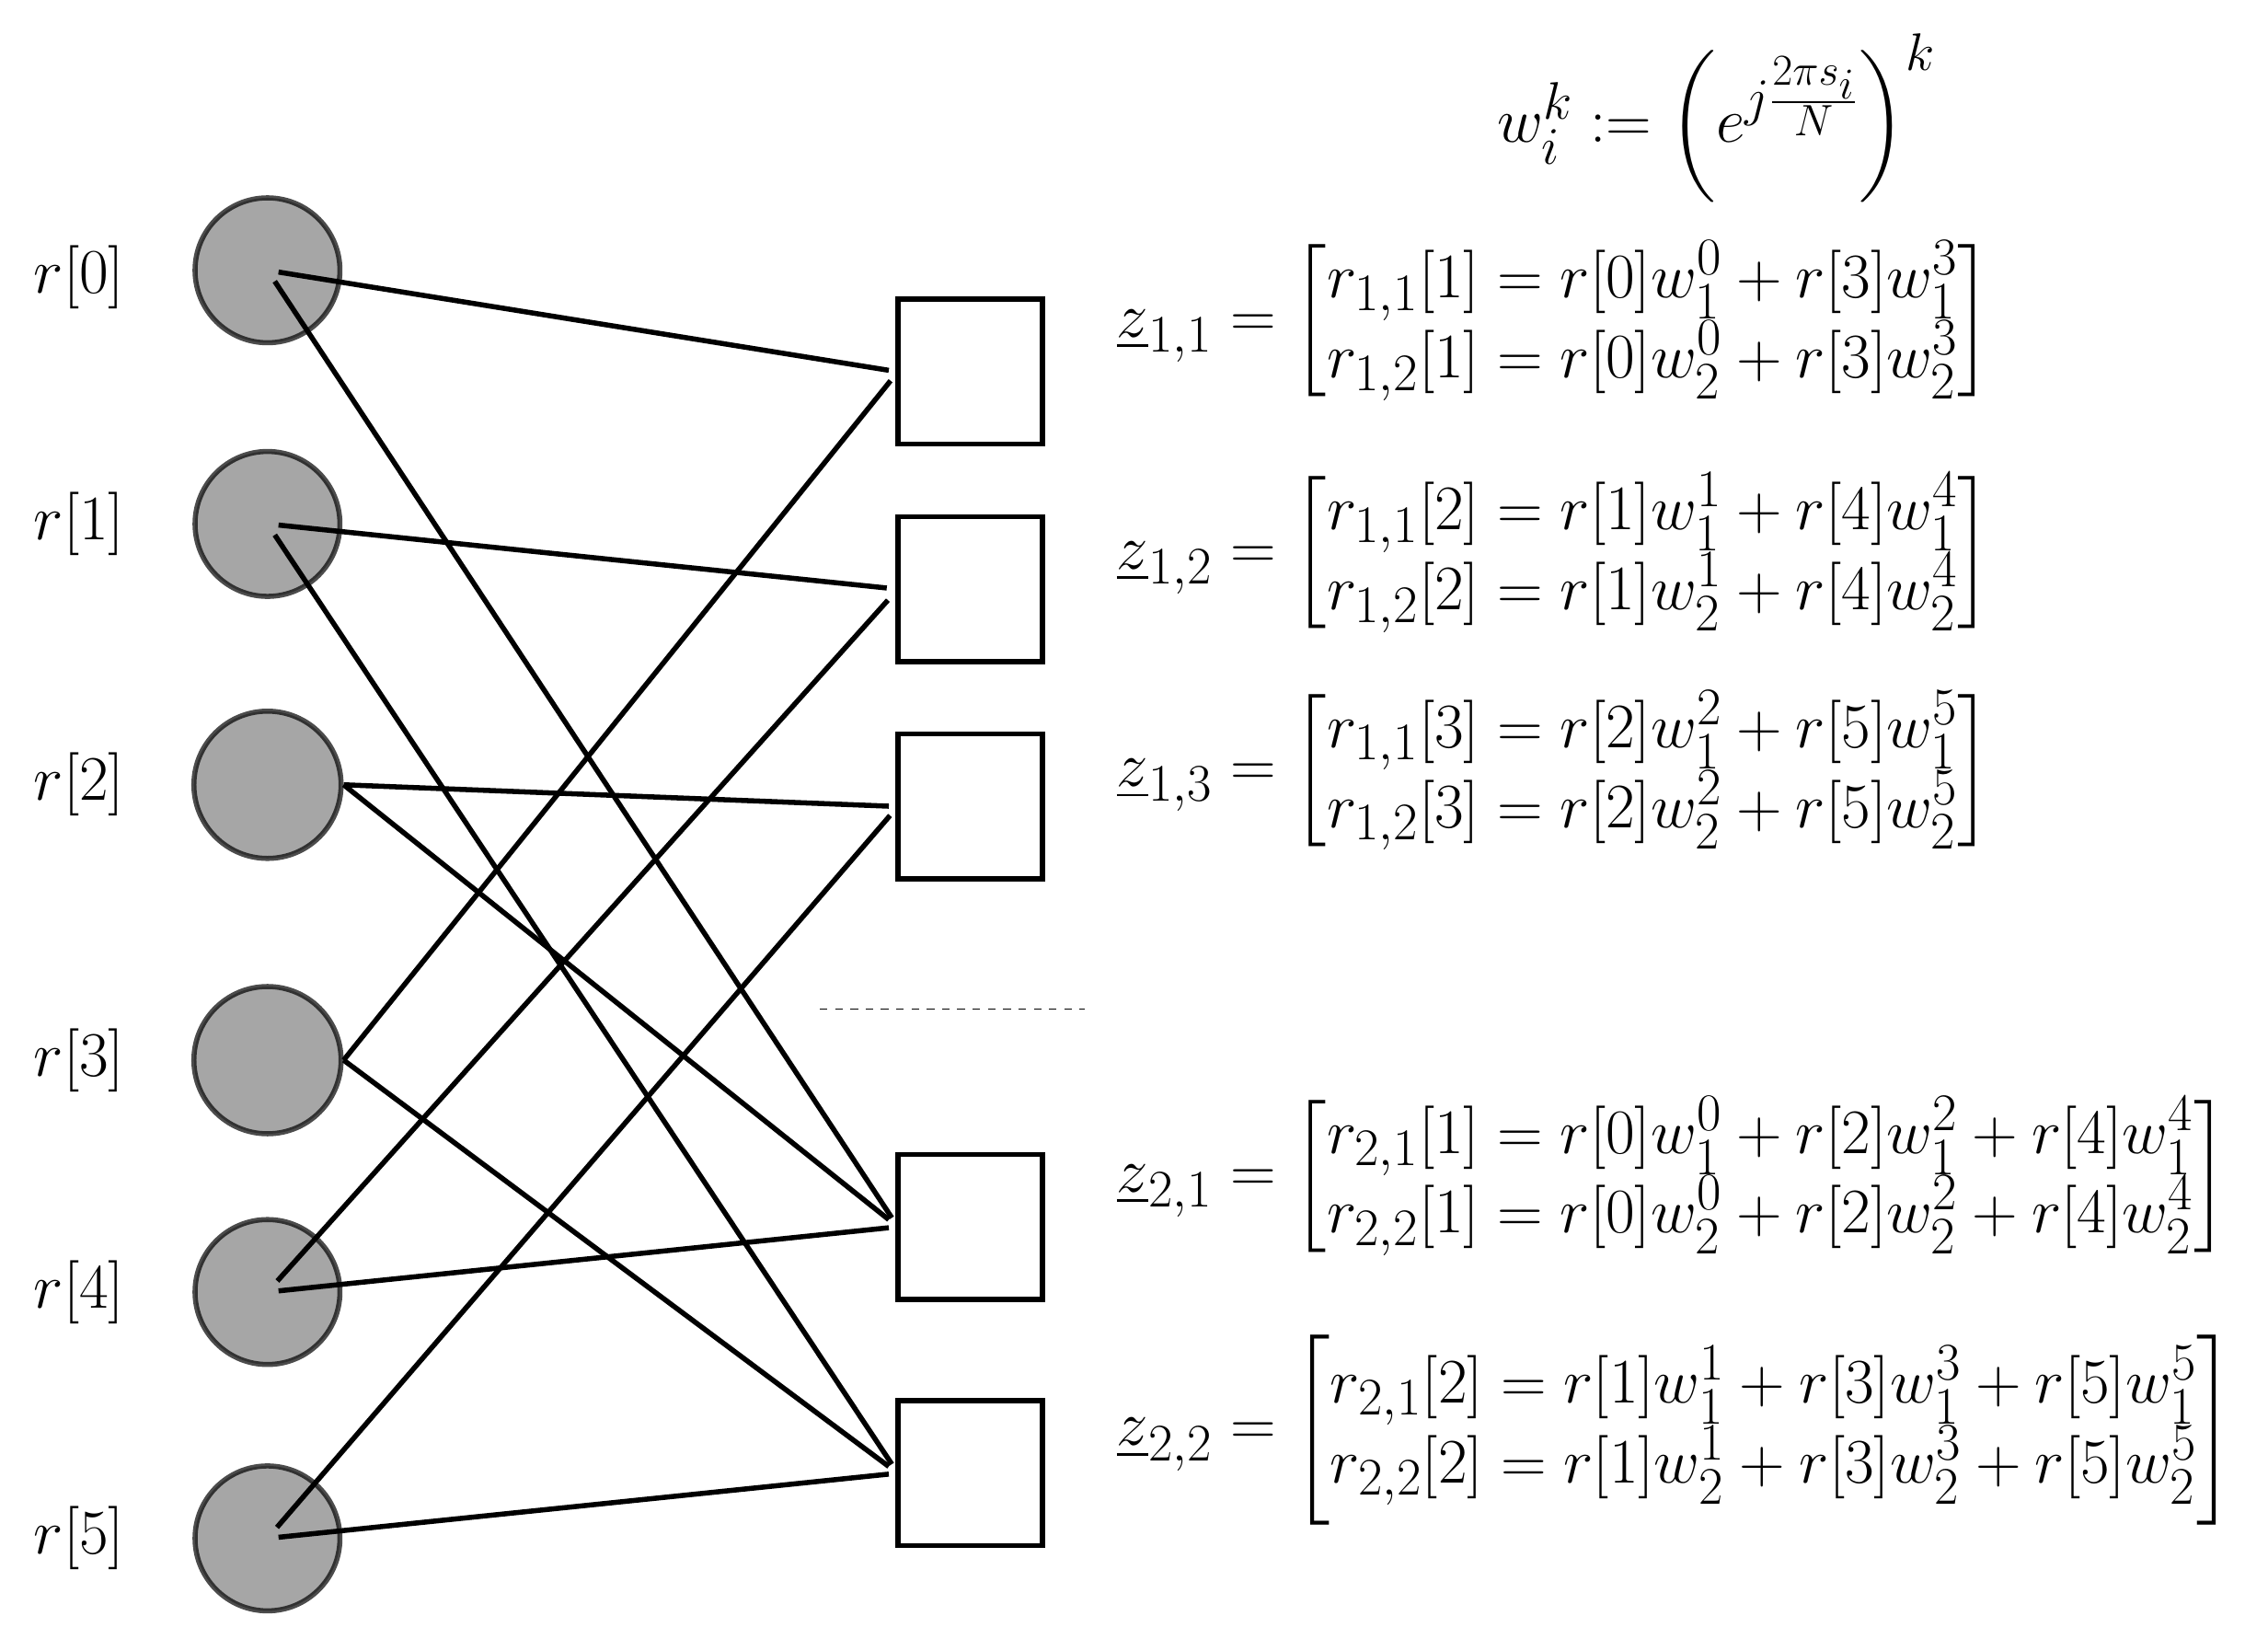
\begin{tikzpicture}

\definecolor{brightturquoise}{rgb}{0.03, 0.91, 0.87}
\definecolor{buff}{rgb}{0.94, 0.86, 0.51}
\definecolor{caribbeangreen}{rgb}{0.0, 0.8, 0.6}
\definecolor{celadon}{rgb}{0.67, 0.88, 0.69}
\definecolor{darktangerine}{rgb}{1.0, 0.66, 0.07}
\definecolor{darkviolet}{rgb}{0.58, 0.0, 0.83}
\definecolor{deepskyblue}{rgb}{0.0, 0.75, 1.0}
\definecolor{amber(sae/ece)}{rgb}{1.0, 0.49, 0.0}
\definecolor{antiquewhite}{rgb}{0.98, 0.92, 0.84}
\definecolor{applegreen}{rgb}{0.55, 0.71, 0.0}
\definecolor{babyblue}{rgb}{0.54, 0.81, 0.94}

\def\nodewidth{0.8in}
\tikzstyle{bit} = [circle, draw, thick,fill=gray,opacity=0.7,line width =2, minimum size=\nodewidth]

% Variable nodes 
\node[bit] (v6) at (-7,-6){};
\node[bit] (v5) at (-7,-2.2) {};
%\draw[thick,fill=gray,line width =2,opacity=0.7]  (-7,-2.2) node (v5) {} ellipse (1 and 1);
\draw [thick,fill=gray,line width =2,opacity=0.7]  (-7,1.4) node (v3) {} ellipse (1 and 1);
\draw  [thick,fill=gray,line width =2,opacity=0.7]  (-7,-9.2) node (v1) {} ellipse (1 and 1);
\draw  [thick,fill=gray,line width =2,opacity=0.7]  (-7,-12.6) node (v1_1) {} ellipse (1 and 1);
\draw  [thick,fill=gray,line width =2,opacity=0.7]  (-7,4.9) node (v1_2) {} ellipse (1 and 1);

%Check nodes
\draw [thick,line width =2] (1.7,4.5) rectangle (3.7,2.5);
\draw [thick,line width =2]  (1.7,1.5) node (v8) {} rectangle (3.7,-0.5);
\draw [thick,line width =2] (1.7,-1.5) rectangle (3.7,-3.5);
\draw [thick,line width =2] (1.7,-7.3) rectangle (3.7,-9.3);
\draw [thick,line width =2] (1.7,-10.7) rectangle (3.7,-12.7);

\node (v2) at (1.7,3.5) {};
\node (v4) at (1.7,-2.5) {};
\node (v7) at (1.7,-8.3) {};
\node (v9) at (1.7,-11.7) {};
\node (v10) at (0.5,-5.3) {};
\node (v11) at (4.4,-5.3) {};



\node at (-9.6,4.8) {\Huge $r[0]$};
\node at (-9.6,1.4) {\Huge $r[1]$};
\node at (-9.6,-2.2) {\Huge $r[2]$};
\node at (-9.6,-6) {\Huge $r[3]$};
\node at (-9.6,-9.2) {\Huge $r[4]$};
\node at (-9.6,-12.6) {\Huge $r[5]$};


\draw [dashed] (v10) edge (v11);
\node [anchor=west] at (4.6,4.2) {\Huge $ \zv_{1,1} = \begin{bmatrix}
	 r_{1,1}[1] = r[0] w_1^{0} + r[3] w_1^{3}  \\
	 r_{1,2}[1] = r[0] w_2^{0} + r[3] w_2^{3} \\
	 \end{bmatrix}$};

\node [anchor=west] at (4.6,1) {\Huge $  \zv_{1,2} = \begin{bmatrix}
	 r_{1,1}[2] = r[1] w_1^{1} + r[4] w_1^{4}\\
	 r_{1,2}[2] = r[1] w_2^{1} + r[4] w_2^{4}\\
	 \end{bmatrix}$};

\node [anchor=west] at (4.6,-2) {\Huge $  \zv_{1,3} = \begin{bmatrix}
	 r_{1,1}[3] = r[2] w_1^{2} + r[5] w_1^{5} \\
	 r_{1,2}[3] = r[2] w_2^{2} + r[5] w_2^{5} \\
	 \end{bmatrix}$};

\node [anchor=west] at (4.6,-7.6) {\Huge $  \zv_{2,1} = \begin{bmatrix}
	 r_{2,1}[1]= r[0] w_1^{0} + r[2] w_1^{2} + r[4] w_1^{4} \\
	 r_{2,2}[1] = r[0] w_2^{0} + r[2] w_2^{2} + r[4] w_2^{4}\\
	 \end{bmatrix}$};

\node [anchor=west] at (4.6,-11.1){\Huge $  \zv_{2,2} = \begin{bmatrix}
	 r_{2,1}[2] =  r[1] w_1^{1} + r[3] w_1^{3} + r[5] w_1^{5} \\ \vspace{3pt}
	 r_{2,2}[2] =  r[1] w_2^{1} + r[3] w_2^{3} + r[5] w_2^{5} \\
	 \end{bmatrix}$};


\draw[thick,line width =2]  (v1_2) edge (v2);
\draw[thick,line width =2]  (v1_2) edge (v7);

\draw[thick,line width =2]  (v3) edge (v9);
\draw[thick,line width =2]  (v5.east) edge (v4);
\node[thick,line width =2] (v12) at (1.7,0.5) {};
\draw[thick,line width =2]  (v3) edge (v12);
\draw[thick,line width =2]  (v5.east) edge (v7);

\draw[thick,line width =2]  (v6.east) edge (v2);
\draw[thick,line width =2]  (v1) edge (v12);
\draw[thick,line width =2]  (v1_1) edge (v4);
\draw[thick,line width =2]  (v6.east) edge (v9);
\draw [thick,line width =2] (v1_1) edge (v9);
\draw [thick,line width =2] (v1) edge (v7);
%\node at (6,7) {\color{blue} \Huge$w_j=e^{j \frac{2\pi s_{j}}{N} }$};
\node at (13,7) { \Huge $w_i^k := \left (  e^{j \frac{2 \pi s_i}{N}}\right )^{k}$};
\end{tikzpicture}
}	
			\end{center}	
			%\caption{Example of a Tanner graph formed in a RSIDFT framework with system parameters being $d=2$, $B=2$, $N=6$, $f_1 = 2$ and $f_2=3$. The variable nodes (colored gray circles) represent the cross-correlation vector $\rv$ and the bin nodes (uncolored white boxes) represent the binned observation vector $\zv_{i,k}$. The figure also illustrates the relationship between $\zv_{i,k}$ and $\rv$.}\label{fig:factorgraph}
		\end{figure}
	\column[]{0.33\columnwidth}
	    \begin{block}{Observations:}
	          $
	    		\zv_{i,k} = \begin{bmatrix}
	    		r_{i,1}[k]\\
	    		r_{i,2}[k]\\
	    		\vdots\\
	    		r_{i,B}[k]
	    		\end{bmatrix}
	    		$
	    	\end{block}
	    	\begin{block}{Decoding- 3 steps}	
	    		\begin{enumerate}
	    			\item Bin Classification
	    			\item Position Identification
	    			\item Peeling Process
	    		\end{enumerate}
	
	    \end{block}
	
		
\end{columns}	
\end{frame}

\begin{frame}\frametitle{Observations}
\begin{align} \nonumber
	    		\zv_{i,k} = \begin{bmatrix}
	    		r_{i,1}[k]\\
	    		r_{i,2}[k]\\
	    		\vdots\\
	    		r_{i,B}[k]
	    		\end{bmatrix}			
            = \begin{bmatrix}
			1 & 1 & \ldots & 1 \\
			\omega^{k}_{2} & \omega^{(k+f_i)}_{2} & \ldots & \omega^{(k+(g_i-1)f_i)}_{2}   \\
			\vdots & \vdots & \ddots & \vdots\\
			\omega^{k}_{B} & \omega^{(k+f_i)}_{B} & \ldots & \omega^{(k+(g_i-1)f_i)}_{B} \\
			\end{bmatrix} \times
			\begin{bmatrix}
			r[k+(0)f_i] \\
			r[k+(1)f_i] \\
			\vdots\\
			r[k+(g_i-1)f_i]
			\end{bmatrix}
			\end{align}

			\begin{figure}[t]
			\begin{center}
				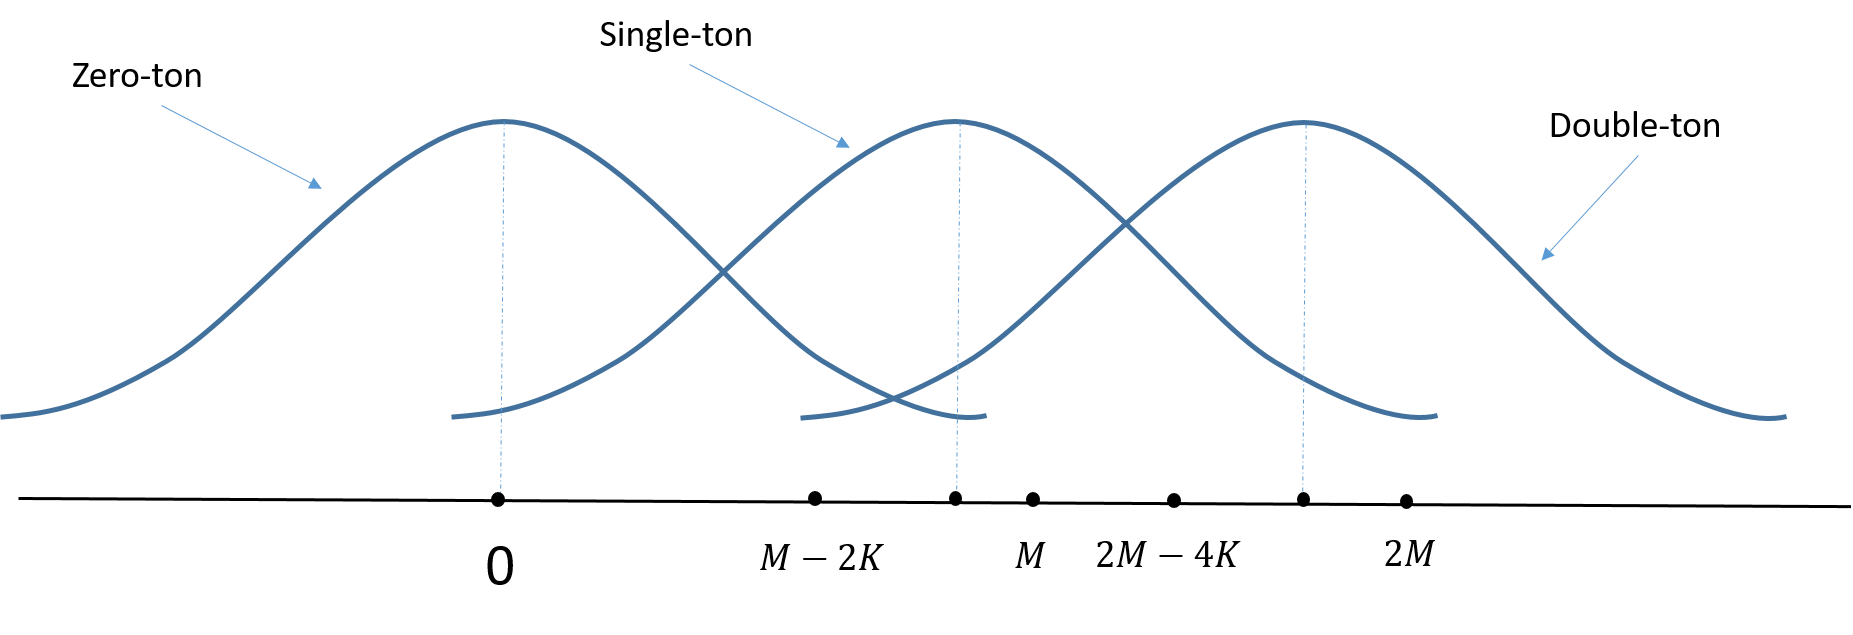
\includegraphics[width=3.5in]{bin_statistics.png}
			\end{center}
		\end{figure}

\end{frame}

\begin{frame}\frametitle{Decoder}

\only<1>{\begin{block}{Bin Classification}
		\begin{itemize}
			\item  Classify each check-node -  Zero-ton / Single-ton / Multi-ton
			\item  {\color{blue} Threshold constraints} on first observation $z_{i,k}[1] = z$
			\item  Threshold varies with $\eta$
			\begin{itemize}
				\item[-] different for exact($\eta=0$) and approximate matching
			\end{itemize}
		\end{itemize}
		\begin{align}
		\label{Eqn:BinClassifApprox} \nonumber
		\widehat{\mc{H}}_{i,j}=
		\begin{cases}
		\mc{H}_z &  	 z/M < \gamma_1\\
		\mc{H}_s &	  \gamma_1 < z/M < \gamma_2  \\
		\mc{H}_d  &    \gamma_2  < z/M <  \gamma_3\\
		\mc{H}_m &      z/M > \gamma_3\\
		\end{cases}
		\end{align}
		where $(\gamma_1,\gamma_2,\gamma_3)=(\frac{1-2\eta}{2},\frac{3-4\eta}{2},\frac{5-6\eta}{2})$
	\end{block}}
	
\only<2>{\vspace{-5pt} \begin{block}{Position Identification}
		\begin{itemize}
			\item 	{\color{blue}Observation:} 	\begin{align} \nonumber
			\zv_{i,k}= \begin{bmatrix}
			1 & 1 & \ldots & 1 \\
			\omega^{k}_{2} & \omega^{(k+f_i)}_{2} & \ldots & \omega^{(k+(g_i-1)f_i)}_{2}   \\
			\vdots & \vdots & \ddots & \vdots\\
			\omega^{k}_{B} & \omega^{(k+f_i)}_{B} & \ldots & \omega^{(k+(g_i-1)f_i)}_{B} \\
			\end{bmatrix} \times
			\begin{bmatrix}
			r[k+(0)f_i] \\
			r[k+(1)f_i] \\
			\vdots\\
			r[k+(g_i-1)f_i]
			\end{bmatrix}
			\end{align}
			
			\item Column that gives {\color {blue} maximum correlation} with the observation\\
			{ \[\boxed{\hat{k} = \underset{k\in\{j+l f_i\}}{\arg \max}~~ \zv^{\dagger}_{i,j} \mathbf{W}[:,l]}\]}
		\end{itemize}
	
		\end{block}}

\only<3>{\begin{block}{Error Probability}
			\begin{align*}
			\mbb{P}(\mathcal{E}_{\text{total}}) & \leq &  \mbb{P}(\mathcal{E}_1)~~~~~ & + & \mbb{P}(\mc{E}_2)~~~~~~~~ & + & \mbb{P}(\mc{E}_3)~~~~~~~~\\
			&\leq & 6e^{-\frac{N^{\mu+\alpha-1}(1-6\eta)^2}{16}}~ & + & 2e^{-N^{\mu+\alpha-1} ~ c_1(\eta)}~ & + &  e^{-c_3 N^{c_4\alpha}}
			\end{align*}
			\[\boxed{	\mbb{P}(\mathcal{E}_{\text{total}}) \rightarrow 0  ~~\text{if}~~  \alpha >1-\mu}\]
		\end{block}
	     }	
\end{frame}
%-------------------------------------------------------------------------------------------------
\begin{frame}{Error Analysis}
	
	\only<1>{\begin{block}{Error Events}
		\begin{itemize}\small
				\item {\color{blue}$\mathcal{E}_1${-\it Bin Classification}}: Bin is wrongly classified
				\item {\color{blue}$\mathcal{E}_2${-\it Pos. Identification}}: Position of singleton is identified wrongly, given a singleton
				\item {\color{blue}$\mathcal{E}_3${-\it Peeling Process}}: Peeling process fails to recover the $L$ significant correlation coefficients, given $\mbb{P}(\mc{E}_1)= \mbb{P}(\mc{E}_2)=0$
		\end{itemize}
	\end{block}
}
	\only<1>{\begin{block}{$\mathcal{E}_1${-\it Bin Classification}}
			\begin{figure}[t]
			\begin{center}
				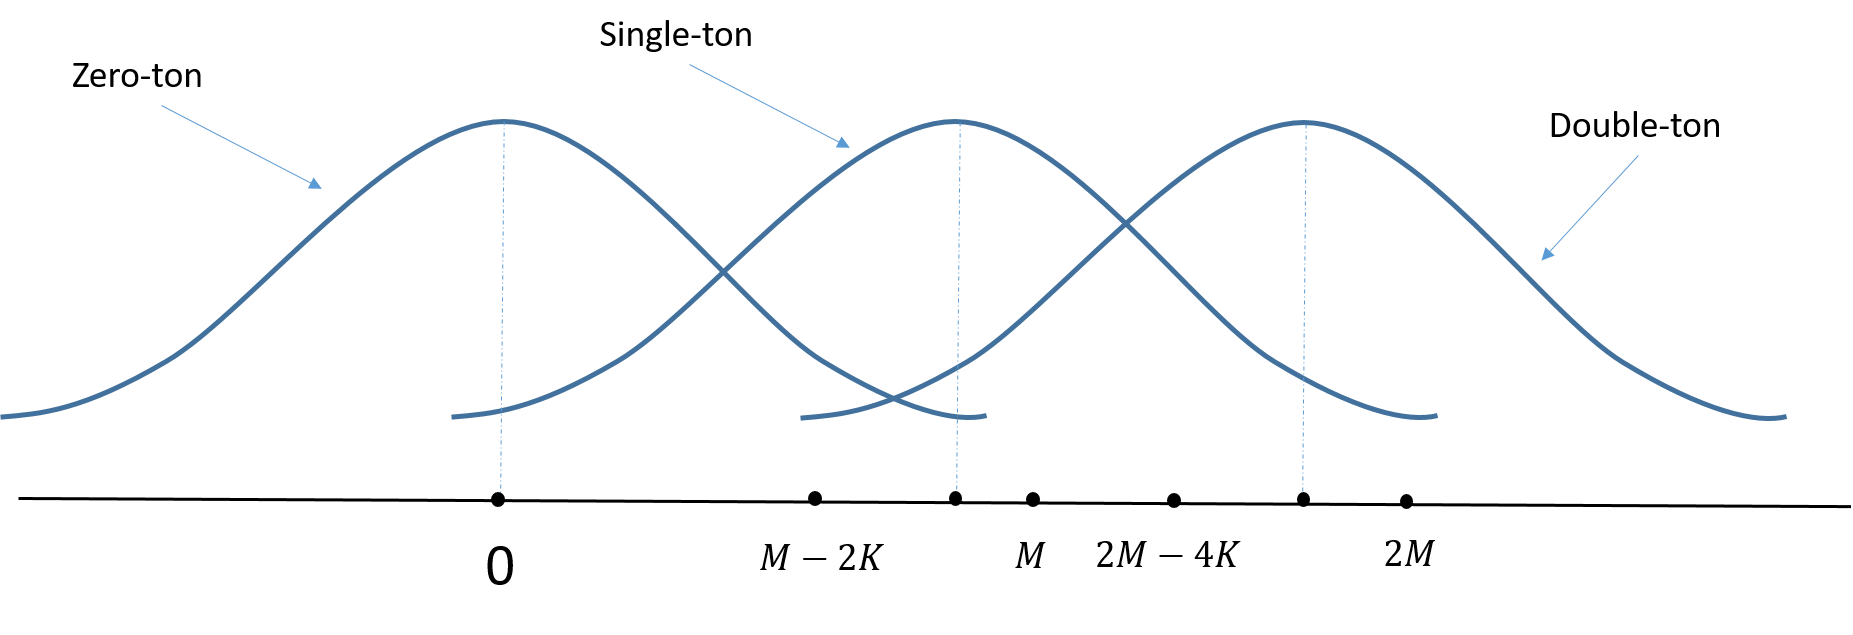
\includegraphics[width=3.5in]{bin_statistics.png}
			\end{center}
		\end{figure}
		\vspace{-20pt}
		
		{\small \begin{align*}
			\mbb{P}[\mc{E}_1] & \leq & \mbb{P}[\mc{E}_1|\widehat{\mc{H}}_{i,j}=\mc{H}_z]~& + &
			\quad \mbb{P}[\mc{E}_1|\widehat{\mc{H}}_{i,j}=\mc{H}_s]~~~~~& + &
			\quad \mbb{P}[\mc{E}_1|\widehat{\mc{H}}_{i,j}=\mc{H}_d \cup \mc{H}_m]\\
			~& = & \mbb{P}[z[1]>\gamma_1] ~& + & (1- \mbb{P}[\gamma_1<z[1]<\gamma_2])  ~& + & \mbb{P}[z[1]<\gamma_2]~~~~~~
			\end{align*}
		}

			\vspace{-17pt}
	\end{block}
	}
\end{frame}
%----------------------------------------------------------------------------------------------------------------
\begin{frame}{Error Analysis}
	
	\only<1,3>{\begin{block}{Error Events}
		\begin{itemize}\small
				\item {\color{blue}$\mathcal{E}_1${-\it Bin Classification}}: Bin is wrongly classified
				\item {\color{blue}$\mathcal{E}_2${-\it Pos. Identification}}: Position of singleton is identified wrongly, given a singleton
				\item {\color{blue}$\mathcal{E}_3${-\it Peeling Process}}: Peeling process fails to recover the $L$ significant correlation coefficients, given $\mbb{P}(\mc{E}_1)= \mbb{P}(\mc{E}_2)=0$
		\end{itemize}
	\end{block}
}

	\only<2>{\begin{block}{$\mathcal{E}_2${-\it Pos. Identification}}
			\begin{itemize}
				\item $\underline{z} =  r[j_p] ~ \wv_{j_p}+ \sum_{k \neq p}n_k \wv_{j_k}$
				\item $\mbb{P}[\mc{E}_2] = \mbb{P}[\wv_{j_p}^{\dagger}\underline{z}< \wv_{j_k}^{\dagger}\underline{z}]$
				\item Mutual Incoherence property to bound the cross-correlation(noise) term
				  \begin{itemize}
				  	\item [-] $\log N$ measurements (shifts) suffices [Pawar'14]
				  \end{itemize}
			\end{itemize}
		     \end{block}
		\begin{align} \nonumber
			\zv_{i,k}= \begin{bmatrix}
			1 & 1 & \ldots & 1 \\
			\omega^{k}_{2} & \omega^{(k+f_i)}_{2} & \ldots & \omega^{(k+(g_i-1)f_i)}_{2}   \\
			\vdots & \vdots & \ddots & \vdots\\
			\omega^{k}_{B} & \omega^{(k+f_i)}_{B} & \ldots & \omega^{(k+(g_i-1)f_i)}_{B} \\
			\end{bmatrix} \times
			\begin{bmatrix}
			r[k+(0)f_i] \\
			r[k+(1)f_i] \\
			\vdots\\
			r[k+(g_i-1)f_i]
			\end{bmatrix}
			\end{align}
	}	
	
		\only<3>{\begin{block}{Error Probability}
			\begin{align*}
			\mbb{P}(\mathcal{E}_{\text{total}}) & \leq &  \mbb{P}(\mathcal{E}_1)~~~~~ & + & \mbb{P}(\mc{E}_2)~~~~~~~~ & + & \mbb{P}(\mc{E}_3)~~~~~~~~\\
			&\leq & 6e^{-\frac{N^{\mu+\alpha-1}(1-6\eta)^2}{16}}~ & + & 2e^{-N^{\mu+\alpha-1} ~ c_1(\eta)}~ & + &  e^{-c_3 N^{c_4\alpha}}
			\end{align*}
			\[\boxed{	\mbb{P}(\mathcal{E}_{\text{total}}) \rightarrow 0  ~~\text{if}~~  \alpha >1-\mu}\]
		\end{block}
	     }	
\end{frame}
%----------------------------------------------------------------------------------------------------------------
\begin{frame}{Error Analysis}
	
	\only<1,3>{\begin{block}{Error Events}
		\begin{itemize}\small
				\item {\color{blue}$\mathcal{E}_1${-\it Bin Classification}}: Bin is wrongly classified
				\item {\color{blue}$\mathcal{E}_2${-\it Pos. Identification}}: Position of singleton is identified wrongly, given a singleton
				\item {\color{blue}$\mathcal{E}_3${-\it Peeling Process}}: Peeling process fails to recover the $L$ significant correlation coefficients, given $\mbb{P}(\mc{E}_1)= \mbb{P}(\mc{E}_2)=0$
		\end{itemize}
	\end{block}
}

	
	\only<2>{	
		\begin{block}{$\mathcal{E}_3${-\it Peeling Process}}
		\begin{itemize}
			\item Tools from Coding Theory to analyze Sparse Graph Codes
			\item Density Evolution to quantify Error Probability
			\item \# of check-nodes is a function of sparsity (query length)
			\item Error probability decays with $N$ - {\small R-FFAST and SAFFRON [Pawar'14, Lee'15]}
		\end{itemize}
		\end{block}
	}	
	
		\only<3>{\begin{block}{Error Probability}
			\begin{align*}
			\mbb{P}(\mathcal{E}_{\text{total}}) & \leq &  \mbb{P}(\mathcal{E}_1)~~~~~ & + & \mbb{P}(\mc{E}_2)~~~~~~~~ & + & \mbb{P}(\mc{E}_3)~~~~~~~~\\
			&\leq & 6e^{-\frac{N^{\mu+\alpha-1}(1-6\eta)^2}{16}}~ & + & 2e^{-N^{\mu+\alpha-1} ~ c_1(\eta)}~ & + &  e^{-c_3 N^{c_4\alpha}}
			\end{align*}
			\[\boxed{	\mbb{P}(\mathcal{E}_{\text{total}}) \rightarrow 0  ~~\text{if}~~  \alpha >1-\mu}\]
		\end{block}
	     }	
\end{frame}
%----------------------------------------------------------------------------------------------------------------
\begin{frame}{Complexity Analysis}
	\begin{block}{Sample Complexity}
		\vspace{-10pt}
		\begin{align*}
		\text{Total \# of samples required (S)} &= O \left(dBN^{\alpha}\right) =   {\color{blue}O(N^{1-\mu}\log N)}
		\end{align*}
	\end{block}
\pause
	\begin{block}{Computational Complexity}
		\begin{equation*}\label{eqn:Rxy_fourier}
		\rv = \underset{\color{red}  \RNum{2} } {\mathcal{F}_{N}^{-1}} \ \{   \mathcal{F}_{N}\{\xv\}  \odot \ \underset{\color{red}  \RNum{1}  }{ \mathcal{F}_{N}\{\yv'\}}  \}
		\end{equation*}
		\vspace{-10pt}
\pause
	\begin{itemize}
		\item {\color{blue}Sketch of Query:}\\ \vspace{5pt}
	 {\small $C_{\color{red}\RNum{1}} \ = \  dB ~
	 ( \underset{\text{Folding} }{\underbrace{N^{\mu}}} + \ \
	 \underset{\text{Shorter FFTs} }{\underbrace{N^{\alpha} \ \log N^{\alpha}}} \ )
	 =  {\color{blue} O(\max(N^{\mu}\log N,N^{1-\mu}\log^2 N)) }$}
\pause
		\item {\color{blue}RSIDFT:} \\	{\small$C_{\color{red} \RNum{2}} =  {d B}  \left (
			\underset{\text{Shorter IFFTs /block/stage} }{\underbrace{ O(N^{\alpha}  \log N^{\alpha})}} \hspace{-3pt}+ \underset{\text{Correlations} }{\underbrace{ L~N^{1-\alpha}}} \right ) = {\color{blue} O(\max(N^{1-\mu}\log^2 N ,N^{\mu+\lambda}\log N)) }$}
	\end{itemize}
	\vspace{10pt}	
	\[\boxed{C_{\text{total}} = \max(C_{\color{red} \text{ \RNum{1}}},C_{\color{red} \text{ \RNum{2}}}) = {\color{blue} O(\max(N^{1-\mu}\log^2 N ,N^{\mu+\lambda}\log N)) }}\]
		
	\end{block}
\end{frame}
%----------------------------------------------------------------------------------------------------------------
\begin{frame}\frametitle{Simulation Results}
\only<1>{\begin{figure}[h!]
		\begin{center}
			
			\resizebox{0.7\textwidth}{!}{% This file was created by matlab2tikz.
%
%The latest updates can be retrieved from
%  http://www.mathworks.com/matlabcentral/fileexchange/22022-matlab2tikz-matlab2tikz
%where you can also make suggestions and rate matlab2tikz.
%
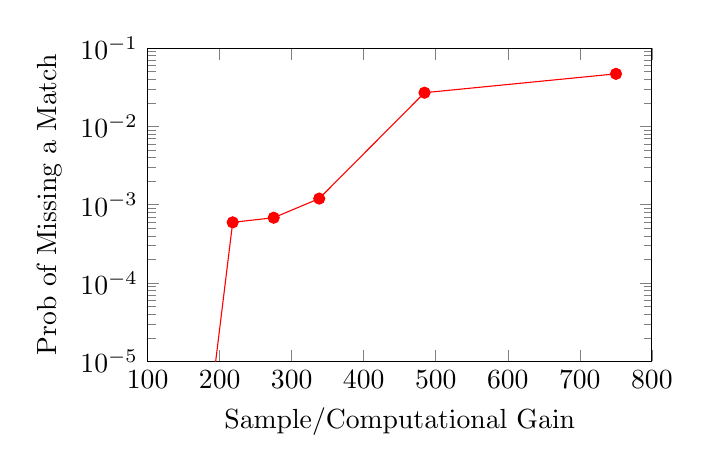
\begin{tikzpicture}

\begin{axis}[%
width=2.521in,
height=1.566in,
at={(0.758in,0.481in)},
scale only axis,
xmin=100,
xmax=800,
xlabel={Sample/Computational Gain},
ymode=log,
ymin=1e-05,
ymax=0.1,
yminorticks=true,
ylabel={Prob of Missing a Match},
axis background/.style={fill=white}
]
\addplot [color=red,solid,mark=*,mark options={solid},forget plot]
  table[row sep=crcr]{%
167.8088	1e-07\\
218.0519	0.0005965\\
274.9922	0.0006834\\
338.1745	0.0012\\
484.384	0.027\\
750.2035	0.047\\
};
\end{axis}
\end{tikzpicture}% }	
				\end{center}
			\caption{Plot of Probability of Missing a Match vs. Sample Gain for Exact Matching of a substring of length $M=10^5$($\mu=0.41$) from a equiprobable  binary \{+1,-1\} sequence of length $N= 10^{12}$, divided into $G=10^{5}$ blocks each of length $\tilde{N}=10^7$. The substring was simulated to repeat in $L=10^6$($\lambda=0.5$) locations uniformly at random.}
	
\end{figure}}

\only<2>{\begin{figure}[h!]
	\begin{center}
		\resizebox{0.7\textwidth}{!}{% This file was created by matlab2tikz.
%
%The latest updates can be retrieved from
%  http://www.mathworks.com/matlabcentral/fileexchange/22022-matlab2tikz-matlab2tikz
%where you can also make suggestions and rate matlab2tikz.
%
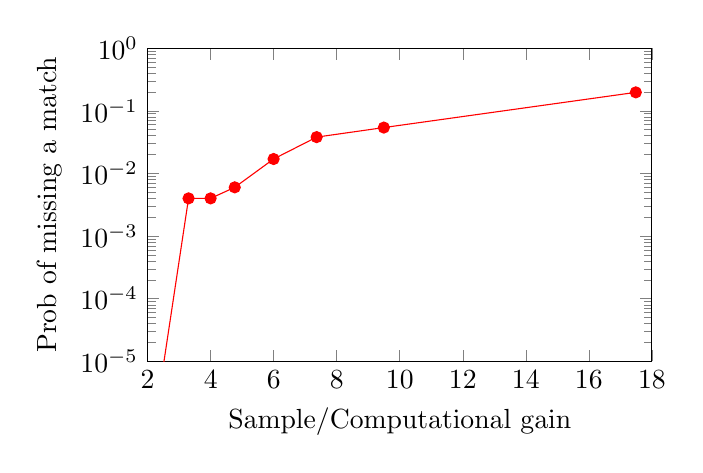
\begin{tikzpicture}

\begin{axis}[%
width=2.521in,
height=1.566in,
at={(0.758in,0.481in)},
scale only axis,
xmin=2,
xmax=18,
xlabel={Sample/Computational gain},
ymode=log,
ymin=1e-05,
ymax=1,
yminorticks=true,
ylabel={Prob of missing a match},
axis background/.style={fill=white}
]
\addplot [color=red,solid,mark=*,mark options={solid},forget plot]
  table[row sep=crcr]{%
2.0985	4e-07\\
3.2978	0.004\\
3.9974	0.004\\
4.7636	0.006\\
5.9963	0.017\\
7.3622	0.038\\
9.4944	0.054\\
17.4904	0.197\\
};
\end{axis}
\end{tikzpicture}% }	
	\end{center}
	\caption{Plot of Probability of Missing a Match vs. Sample Gain for Exact Matching of a substring of length $M=10^3$($\mu=0.25$) from a equiprobable  binary \{+1,-1\} sequence of length $N= 10^{12}$, divided into $G=10^{6}$ blocks each of length $\tilde{N}=10^6$. The substring was simulated to repeat in $L=10^6$($\lambda=0.5$) locations uniformly at random.}
	
\end{figure}}
\end{frame}

\begin{frame}{Secure Pattern Matching}
v\begin{figure}
  \centering
  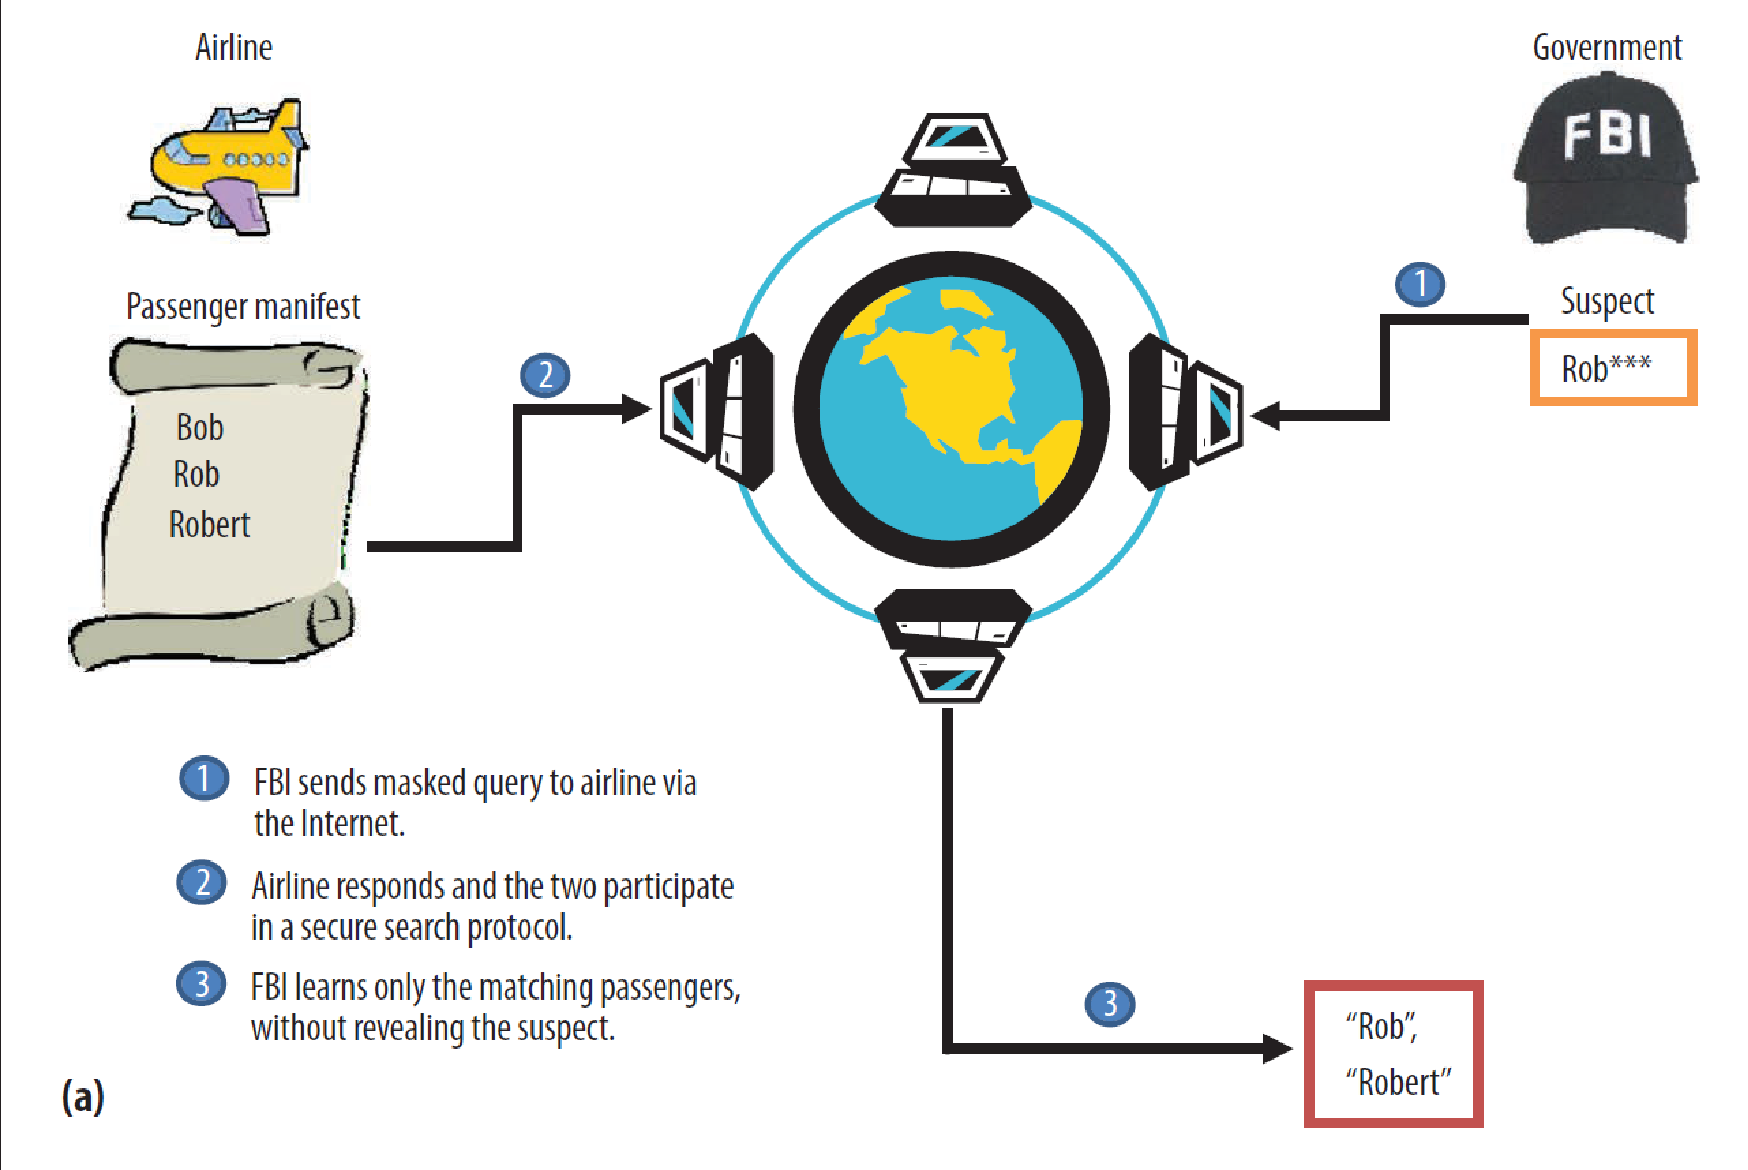
\includegraphics[width=4.0in]{airline}
\end{figure}
\end{frame}

\begin{frame}{Secure Pattern Matching}
\begin{figure}
  \centering
  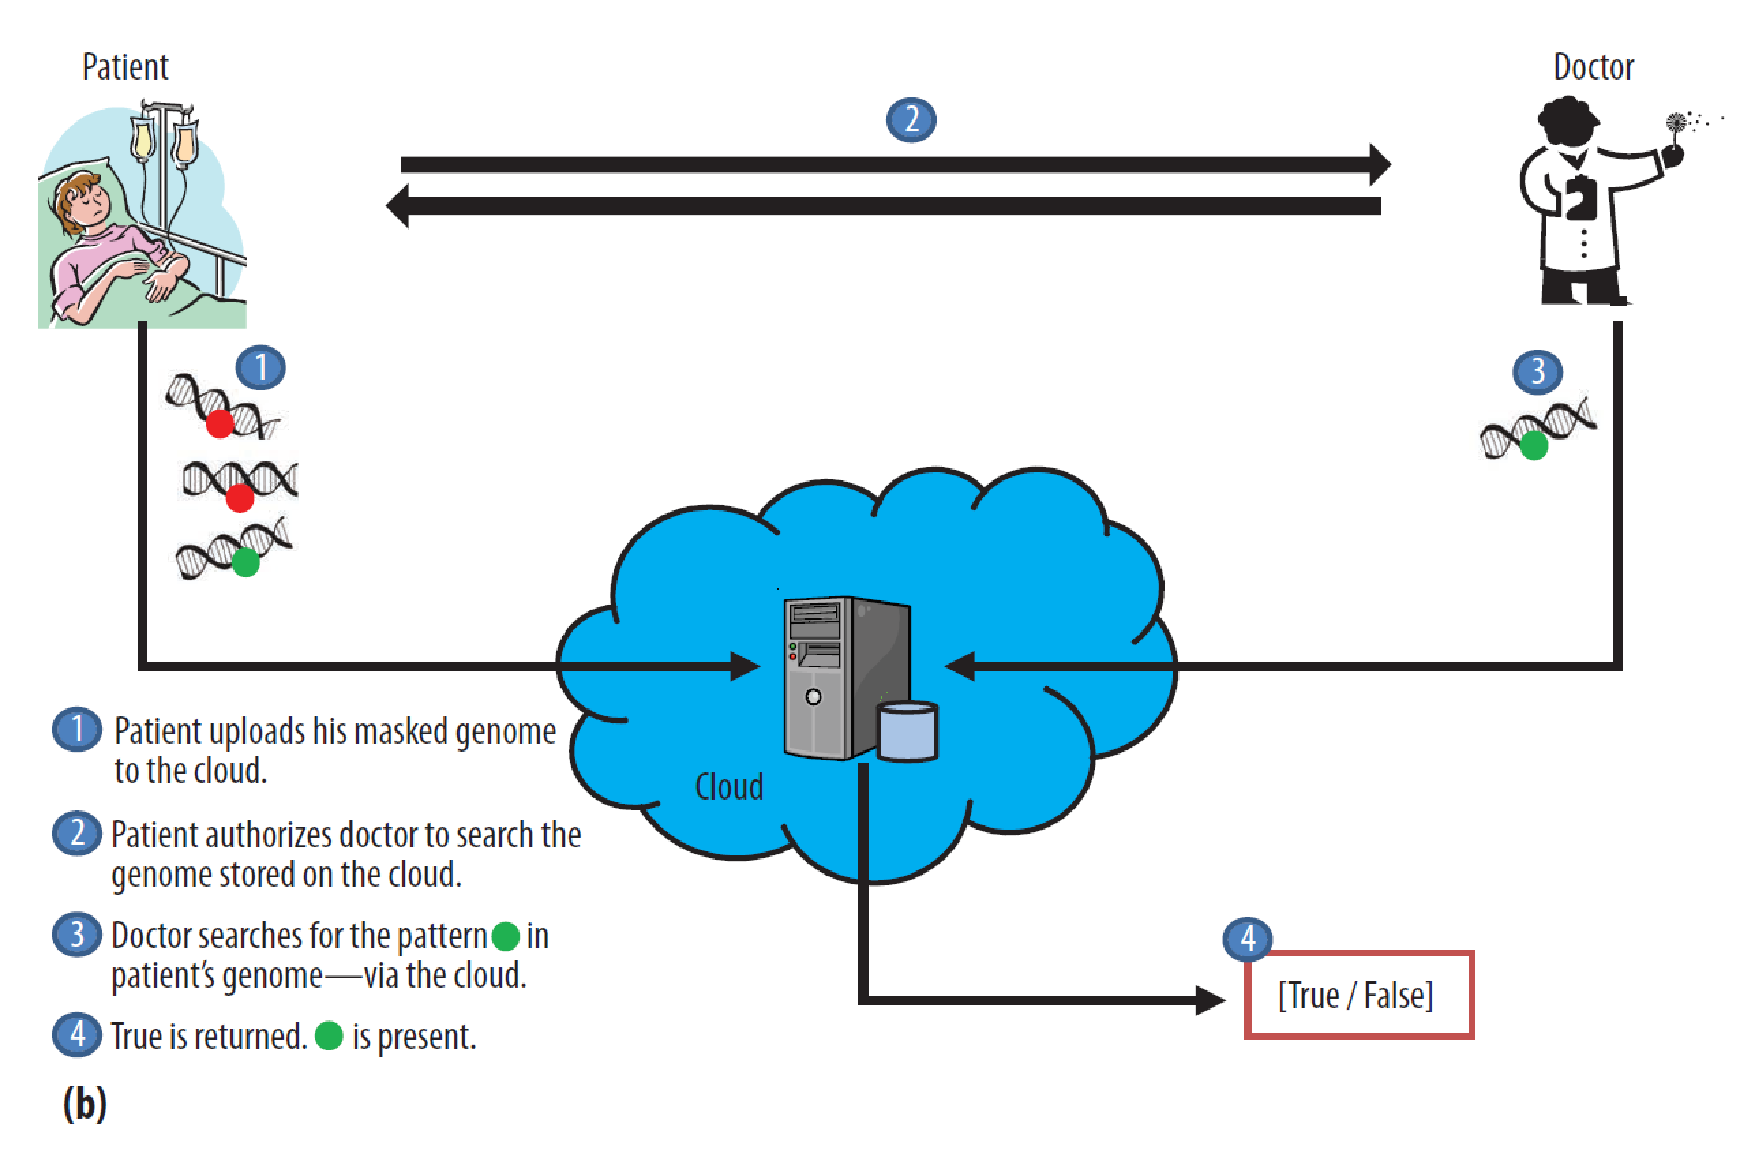
\includegraphics[width=4.0in]{doctorpatient}
\end{figure}
\end{frame}
%--------------------------------------------------------------------------------------
%-----------------References --------------------
%\begin{frame}[allowframebreaks]
%\frametitle{References}%in case more than 1 slide needed
%	{\footnotesize
%		\bibliographystyle{ieeetr}
%		\bibliography{sparseestimation}	}
%\end{frame}


%---------------------------------------------------------------------------------------
\begin{frame}\frametitle{Questions?}
	\begin{figure}[t]
		\centering
		
\includegraphics[width=2.8in]{questions}
	\end{figure}
	\centering
	\color{blue}
	\Huge{Thank you!}
\end{frame}

\end{document} 